\documentclass[12pt,twoside,a4paper]{article}
\usepackage[utf8]{inputenc}

\usepackage[colorlinks=false]{hyperref}

%\usepackage[fleqn]{amsmath}
\usepackage{import}
\usepackage{amsmath, nccmath}
\usepackage{mathtools}
\usepackage{amsfonts}
\usepackage{bm}
\usepackage{multirow}
\usepackage{stmaryrd}
\usepackage{cleveref}
\usepackage{float}
\usepackage{booktabs}
\usepackage[nottoc,numbib,notlof,notlot]{tocbibind}
\usepackage{tikz}
\usepackage{pgfplots}
\pgfplotsset{compat=1.9}
\usepackage{algorithm}
\usepackage{algpseudocode}
\usepackage{setspace}
\usepackage{placeins}
\usepackage[margin=1cm,labelfont=bf]{caption}
\usepackage[margin=0.25cm,labelfont=bf]{subcaption}
\usepackage{dsfont}
\usepackage{booktabs}
\usepackage{rotating}
\usepackage{lscape}
\usepackage{diagbox}
\usepackage{comment}


\renewcommand\thesubfigure{\roman{subfigure}}

\usepackage{fancyhdr}
\setlength{\headheight}{15.34767pt}
\pagestyle{fancy}
\fancyhf{}
\fancyhead[LE,RO]{\rightmark}
\fancyhead[RE,LO]{\leftmark}
\fancyfoot[C]{\thepage}

\fancypagestyle{contents}{% define a custom header OPTION 1 to be applied to specific pages
    \fancyhf{}
    \fancyhead[RE,LO]{\leftmark}
    \fancyfoot[C]{\thepage}
}


\numberwithin{equation}{section}

\usepackage{placeins}
\usepackage{graphicx}
\graphicspath{ {./Images/} }
\usepackage[margin=1.1in]{geometry}
\renewcommand{\arraystretch}{1.7}

\doublespacing

\newcommand{\ra}[1]{\renewcommand{\arraystretch}{#1}}

\usepackage[toc,page]{appendix}

\usepackage[backend=biber, style=numeric-comp, sorting=none, uniquename=init, giveninits=true, natbib=true, doi=false,url=false,isbn=false]{biblatex}
\addbibresource{references.bib}
\setcounter{biburlnumpenalty}{100}
\setcounter{biburlucpenalty}{100}
\setcounter{biburllcpenalty}{100}

\DeclareSourcemap{
    \maps{
        % Replace '{\_}', '{_}' or '\_' with just '_' in doi field
        \map{
            \step[
                fieldsource=doi,
                match=\regexp{\{\\\_\}|\{\_\}|\\\_},
                replace=\regexp{\_}
            ]
        }
        % Replace '{\_}', '{_}' or '\_' with just '_' in url field
        \map{
            \step[
                fieldsource=url,
                match=\regexp{\{\\\_\}|\{\_\}|\\\_},
                replace=\regexp{\_}
            ]
        }
    }
}

\newbibmacro{string+doiurlisbn}[1]{%
  \iffieldundef{doi}{%
    \iffieldundef{url}{%
      #1%
    }{%
      \href{\thefield{url}}{#1}%
    }%
  }{%
    \href{http://dx.doi.org/\thefield{doi}}{#1}%
  }%
}

\DeclareFieldFormat{title}{\usebibmacro{string+doiurlisbn}{\mkbibemph{#1}}}
\DeclareFieldFormat[article,incollection]{title}%
    {\usebibmacro{string+doiurlisbn}{\mkbibquote{#1}}}


\allowdisplaybreaks

\begin{document}

\begin{titlepage}
    \begin{center}
        \vspace*{1cm}

        \LARGE
        \textbf{Kernel-independent fast multipole method for the computation of large regularized Stokeslet systems}

        \normalsize
        \vspace{0.5cm}
        Analysis of the Kernel-independent fast multipole method for use in bio-fluids
        
        \vspace{1.5cm}
        
        \textbf{Samuel Walker}\\
        Supervisor : D.J Smith \\
        Co-Supervisor : T.D Montenegro-Johnson
        
        \vfill
        
        \vspace{0.8cm}
        
        
\includegraphics[width=0.2\textwidth]{BhamLogo.png}\\
        
        \normalsize
        School of Mathematics\\
        University of Birmingham\\
        United Kingdom\\
        May 2022
            
    \end{center}
\end{titlepage}





\pagestyle{fancy}
\fancyhf{}
\fancyhead[LE,RO]{\rightmark}
\fancyhead[RE,LO]{\leftmark}
\fancyfoot[C]{\thepage}

\newpage
\section*{Abstract}
With the aim to form a fast mesh-free method for solving Stokes flow in biological fluid dynamics, we consider options to accelerate the method of regularised stokeslets. Although simple to implement, the method of regularised stokeslets comes with a large computational cost as traditional methods require the creation of large dense matrices which quickly become computationally challenging to work with. We consider the use of the Kernel Independent Fast Multipole method (KIFMM) to compute the interactions between regularised stokeslet points. In this case, we show that the KIFMM method can be used to quickly and efficiently evaluate the matrix-vector product when compared to the direct product method. We then consider cases which require the solving of linear systems involving the stokeslet matrix. For the case of augmented problems such as the force-free swimming problem, we derive an appropriate preconditioner to aid convergence when using the Generalized Minimal RESidual method (GMRES). Our main contribution is the adaptation of the KIFMM method to use nearest neighbour interpolation in order to reduce the overall number of degrees of freedom in our system and aid overall computation times. This method shows promise, dramatically reducing computation times for certain systems, however more work is needed to form an optimal method for problems. 

\newpage
\section*{Acknowledgements}
I would like to thank the following people for helping me through this project and allowing me to write something I am incredibly proud of. Thank you to my supervisor Professor Dave Smith whose expertise and insight guided me throughout the project. To my parents and Nick Wicks who have proofread so many drafts of this paper. And finally to the University of Birmingham's BlueBEAR HPC service for the generous amounts of computing power which allowed for the computations in this project to be possible. 


\begin{singlespace}
\pagestyle{contents}
\newpage
{
  \hypersetup{hidelinks}
  \tableofcontents
}

\newpage
\listoffigures
\newpage
\listoftables
\listofalgorithms
\end{singlespace}

\pagestyle{fancy}

\newpage
\section{Introduction}
At the scale of microorganism fluid dynamics plays an important and defining role in the evolution and behaviour of these cells particularly in the interactions of multiple cells. Experiments have shown that at high enough density the collective motion of cells can form unique and complex arrangements which define and explain their evolutionary traits. While experiments on microorganism provide an understanding into the larger biological systems, mathematical models allows of a deeper understanding of the underlying physics. 

The biological relevance of flows at this scale has motivated over 150 years of research into understanding fluids at this scale. Originally studied by Stokes \cite{Stokes2010OnPendulums}, the steady-state Stokes equations \cref{eq:StokesFlow} govern flows at this scale where viscous forces dominate over the inertial forces. While analytical analysis has been used to make significant progress into understand Stokes flow in particular the analysis of flows around sperm like swimmers \cite{Hancock1953TheLiquids,GRAY1955TheSpermatozoa,Taylor1951AnalysisOrganisms}. However although the analysis done analytically provides significant progress into understanding biological flows they are unable to provide results to more complex and relevant problems which typically involve multiple swimmers and large amplitude motion. Most recent work on stokes flows has been focused on methods to computationally solve the steady state Stokes equations. 

As the Stokes equations are linear and elliptical partial differential equations they can be formulated in terms of a boundary integral equation; where typical method to solve differently equation such as finite element method would require the discretisation over the whole volume, particularly given the infinite volumes we will be concerning, the equation can be solve as a integral over the boundary. This reduction dimension vastly reduces the size of the problem which is obtained from the discretisation of the problem and removes the need to mesh the whole volume. Many numerical method have been derived to solve the boundary integral equations, including a boundary element method (BEM) for stokes flow developed by Phan-Thien et al \cite{Tran-Cong1987APropulsion}, have been use to model these systems. While these methods are both accurate and efficient they present two challenges particularly for researchers who are not computational specialists. The first challenge is the need to generate a smooth surface mesh on the boundary of the object. While this is relatively easy for simple geometry it is not often obvious how these meshes can be formed for more complex moving geometry. While automatic mesh generators have allowed for simpler implantation of BEM methods they do not provide a robust and efficient solution to all geometries and often lead to unnecessary calculations where the mesh has been refined  beyond what is necessary. The second problem arises from the singular solution (\cref{eq:singularsolutions}) which arise from the is the requirement for semi-analytical quadrature method which are hard to implement effectively. While libraries such as BEMLIB \cite{BEMLIB} have mostly eliminated this problem for the end user it does add a layer of complexity to the calculations.

In order to address both these problems Cortez et al \cite{Cortez2001,Cortez2005} introduced the method of regularised stokeslet which both removes the need for a connected mesh and removes the singularities in the solutions. The core idea is the replacement of the stokes flow formed by a Dirac delta force-per-unit-volume distribution, with a flow formed by cutoff function. We review this method in \cref{sec:MRS} including the derivation of its boundary integral equation. While this method proves very easy to implement it does come at a computational cost, where the number of degrees of freedom needed to discrete the boundary is significantly higher than typical BEM implementations in order to achieve similar levels of accuracy. This is further compounded by the coupling of the discretisation spacing with the regularisation parameter which as shown in \cref{sec:MRS} furthers the need refine the surface discretisation. 

In chapters \cref{sec:Nbody,sec:KIFMM} we will consider how we can consider solving Stokes flow using the method of regularised stokeslets as a $N$-body problem and how it is possible to reduce the traditional $\mathcal{O}(N^2)$ complexity of the problem to $\mathcal{O}(N)$ though the use of Fast summation methods, in particular the Kernel Independent Fast Multipole Method (KIFMM) developed by Ying, Biros and Zorin \cite{Ying2004} which we review in detail in \cref{sec:KIFMM}. We will also consider an alternative `nearest neighbour' discretisation by Smith \cite{Smith2018AEquation} in \cref{sec:NEAREST} which aims to retain the meshfree nature  of the standard implementation while dramatically reducing the computational cost of the method. The main contribution of this paper is the formulation of a hybrid method which uses both nearest neighbour interpolation to reduce the overall number of degrees of freedom and the KIFMM algorithm to quickly evaluate the particle to particle interactions. Finally \cref{sec:NumericalSims} explores how KIFMM and the hybrid KIFMM NEAREST methods can be use to solve problems in stokes flow, in particular swimming problems the motion of multiple swimmers can found from there from given given boundary deformation and force/moment balance. This promotes the use of GMRES and an appropriate preconditioner based on work by Rostami and Olson \cite{Rostami2019FastBiofluids}.


\FloatBarrier
\section{Method of regularised stokeslets} \label{sec:MRS}
\subsection{Stokes flow}
When we analyse many physical systems, particularly in microscopic biology, we find that the inertial forces within the fluid are small in comparison to that of the viscous terms. In these cases we can take the limit of the Navier-Stokes equation [WHY] (\cref{eq:NavierStokes}) where $Re=\rho u L/\mu \to 0 $ \cite{Trombley2019BasicFlows}. In this limit, we obtain the steady-state Stokes equations in two or three dimensions as 
\begin{subequations}
\label{eq:StokesFlow}
\begin{align}
    \mu\Delta\boldsymbol{u} &= \nabla p - \boldsymbol{F} \label{eq:StokesFlow1} \\
    \nabla \cdot \boldsymbol{u} &= 0 \label{eq:StokesFlow2}
\end{align}
\end{subequations}
where $\bm{u}$ is the velocity of the fluid, $\bm{F}$ is the external body force, $p$ is the pressure and $\mu$ is the fluid viscosity.

Stokes flows occur either where $\mu$ is large or at small length scales where $L$ (typical scale of the system) is small, such as when analysing the flows around cells, microorganisms, or small capillaries \cite{Blake1972AOrganisms, Higdon1979APropulsion, Smith2009MathematicalFluids}. Stokes flow is not only useful in modelling flows in microbiology but also in non-biological systems, such as industrial applications with small scale flows and complex boundaries \cite{Liron1978StokesPipe, Liron1976StokesPlates}.

When looking for solutions to the Stokes equation \cref{eq:StokesFlow} there are many different techniques we can use, both numerically and analytically. We will be focusing on the use of the Green's function of Stokes flow called a stokeslet \cite{Pozrikidis1992BoundaryFlow,Hancock1953TheLiquids} or Oseen tensor \cite{Oseen1927NeuereHydrodynamik}. The stokeslet represents a fundamental solution for the velocity of the fluid given that an external force $\bm{F}$ acts on the fluid at a single point $\bm{F} = \bm{f_0}\delta(\bm{x})$ \cite{Hancock1953TheLiquids, Batchelor2000AnDynamics}.
Through similar methods to those shown later for deriving the regularised stokeslet Equation, (\cref{eq:regstokeslet2}) we can derive the singular fundamental solutions to the Stokes equations as
\begin{equation}
\label{eq:singularsolutions}
\begin{aligned}
    S_{j k}(\bm{x}, \bm{y}) &= \frac{\delta_{j k}}{r}+\frac{\left(x_{j}-y_{j}\right)\left(x_{k}-y_{k}\right)}{r^{3}} \\
    P_{k}(\bm{x}, \bm{y}) &= \frac{x_{k}-y_{k}}{r^{3}} \\
    T_{ijk}(\bm{x}, \bm{y}) &= \frac{-6\left(x_{i}-y_{i}\right)\left(x_{j}-y_{j}\right)\left(x_{k}-y_{k}\right)}{r^5}
\end{aligned}
\end{equation}
Where $r=|\bm{x}-\bm{y}|$.

We can then find the velocity $\bm{u}$ and pressure $p$ at a point $\bm{x}$ through the equations
\begin{equation*}
    \bm{u} = (8 \pi \mu)^{-1} \left(S_{1j},S_{2j},S_{3j}\right)f_{0,j}, \quad p = (8 \pi)^{-1} P_k f_{0,j} 
\end{equation*}
where $\bm{f_{0}}$ is the force per unit area exerted by the fluid on the surface, concentrated at the point $\bm{y}$. 


\subsection{Regularising the stokeslet}
While the singular stokeslet provides a useful mechanism to solve boundary integral equations, the solutions contain singular points which prove computationally challenging unless careful consideration of the quadrature discretisation is considered as we cannot evaluate close to these singular points.

\begin{figure}[ht]
    \centering
    \resizebox{.6\linewidth}{!}{% This file was created by matlab2tikz.
%
%The latest updates can be retrieved from
%  http://www.mathworks.com/matlabcentral/fileexchange/22022-matlab2tikz-matlab2tikz
%where you can also make suggestions and rate matlab2tikz.
%
\begin{tikzpicture}

\begin{axis}[%
width=4.521in,
height=3.566in,
at={(0.758in,0.481in)},
scale only axis,
xmin=0,
xmax=0.025,
xlabel style={font=\color{white!15!black}},
xlabel={r},
ymin=0,
ymax=600000,
ytick={0,100000,200000,300000,400000,500000,600000},
yticklabels={\empty},
ylabel style={font=\color{white!15!black}},
ylabel={$\phi{}_\epsilon\text{(r)}$},
axis background/.style={fill=white},
axis x line*=bottom,
axis y line*=left,
legend style={legend cell align=left, align=left, draw=white!15!black}
]
\addplot [color=black]
  table[row sep=crcr]{%
0	176838.825657661\\
2.5025025025025e-05	176837.102958392\\
5.00500500500501e-05	176831.934990042\\
7.50750750750751e-05	176823.322140968\\
0.0001001001001001	176811.265058366\\
0.000125125125125125	176795.764648167\\
0.00015015015015015	176776.822074908\\
0.000175175175175175	176754.438761544\\
0.0002002002002002	176728.616389237\\
0.000225225225225225	176699.356897096\\
0.00025025025025025	176666.662481879\\
0.000275275275275275	176630.535597662\\
0.0003003003003003	176590.978955459\\
0.000325325325325325	176547.99552281\\
0.00035035035035035	176501.588523328\\
0.000375375375375375	176451.761436205\\
0.0004004004004004	176398.517995683\\
0.000425425425425425	176341.862190484\\
0.00045045045045045	176281.798263201\\
0.000475475475475476	176218.330709652\\
0.0005005005005005	176151.464278195\\
0.000525525525525526	176081.203969007\\
0.000550550550550551	176007.55503332\\
0.000575575575575576	175930.522972626\\
0.000600600600600601	175850.113537839\\
0.000625625625625626	175766.332728426\\
0.000650650650650651	175679.18679149\\
0.000675675675675676	175588.682220831\\
0.000700700700700701	175494.825755958\\
0.000725725725725726	175397.624381071\\
0.000750750750750751	175297.085324005\\
0.000775775775775776	175193.216055138\\
0.000800800800800801	175086.024286264\\
0.000825825825825826	174975.517969433\\
0.000850850850850851	174861.705295753\\
0.000875875875875876	174744.594694153\\
0.000900900900900901	174624.194830126\\
0.000925925925925926	174500.514604421\\
0.000950950950950951	174373.563151714\\
0.000975975975975976	174243.349839237\\
0.001001001001001	174109.88426538\\
0.00102602602602603	173973.176258258\\
0.00105105105105105	173833.235874244\\
0.00107607607607608	173690.073396472\\
0.0011011011011011	173543.699333309\\
0.00112612612612613	173394.124416795\\
0.00115115115115115	173241.359601048\\
0.00117617617617618	173085.416060649\\
0.0012012012012012	172926.305188982\\
0.00122622622622623	172764.038596561\\
0.00125125125125125	172598.628109313\\
0.00127627627627628	172430.085766842\\
0.0013013013013013	172258.423820657\\
0.00132632632632633	172083.654732381\\
0.00135135135135135	171905.791171923\\
0.00137637637637638	171724.84601563\\
0.0014014014014014	171540.832344409\\
0.00142642642642643	171353.763441819\\
0.00145145145145145	171163.652792149\\
0.00147647647647648	170970.514078457\\
0.0015015015015015	170774.361180591\\
0.00152652652652653	170575.208173186\\
0.00155155155155155	170373.069323637\\
0.00157657657657658	170167.959090044\\
0.0016016016016016	169959.892119137\\
0.00162662662662663	169748.883244184\\
0.00165165165165165	169534.947482866\\
0.00167667667667668	169318.100035138\\
0.0017017017017017	169098.356281068\\
0.00172672672672673	168875.731778653\\
0.00175175175175175	168650.24226162\\
0.00177677677677678	168421.903637199\\
0.0018018018018018	168190.731983885\\
0.00182682682682683	167956.743549178\\
0.00185185185185185	167719.954747305\\
0.00187687687687688	167480.382156926\\
0.0019019019019019	167238.042518822\\
0.00192692692692693	166992.952733564\\
0.00195195195195195	166745.129859173\\
0.00197697697697698	166494.591108756\\
0.002002002002002	166241.353848133\\
0.00202702702702703	165985.435593451\\
0.00205205205205205	165726.854008777\\
0.00207707707707708	165465.626903683\\
0.0021021021021021	165201.772230818\\
0.00212712712712713	164935.308083468\\
0.00215215215215215	164666.2526931\\
0.00217717717717718	164394.624426902\\
0.0022022022022022	164120.441785305\\
0.00222722722722723	163843.723399501\\
0.00225225225225225	163564.488028947\\
0.00227727727727728	163282.754558864\\
0.0023023023023023	162998.541997722\\
0.00232732732732733	162711.869474723\\
0.00235235235235235	162422.756237274\\
0.00237737737737738	162131.221648449\\
0.0024024024024024	161837.285184455\\
0.00242742742742743	161540.966432079\\
0.00245245245245245	161242.285086141\\
0.00247747747747748	160941.260946937\\
0.0025025025025025	160637.913917676\\
0.00252752752752753	160332.264001916\\
0.00255255255255255	160024.331301\\
0.00257757757757758	159714.136011478\\
0.0026026026026026	159401.698422543\\
0.00262762762762763	159087.038913449\\
0.00265265265265265	158770.177950942\\
0.00267767767767768	158451.136086677\\
0.0027027027027027	158129.933954646\\
0.00272772772772773	157806.592268603\\
0.00275275275275275	157481.131819481\\
0.00277777777777778	157153.573472828\\
0.0028028028028028	156823.938166227\\
0.00282782782782783	156492.246906729\\
0.00285285285285285	156158.520768286\\
0.00287787787787788	155822.780889186\\
0.0029029029029029	155485.048469492\\
0.00292792792792793	155145.344768488\\
0.00295295295295295	154803.691102126\\
0.00297797797797798	154460.108840481\\
0.003003003003003	154114.619405207\\
0.00302802802802803	153767.244267006\\
0.00305305305305305	153418.004943097\\
0.00307807807807808	153066.922994699\\
0.0031031031031031	152714.02002451\\
0.00312812812812813	152359.317674208\\
0.00315315315315315	152002.837621948\\
0.00317817817817818	151644.601579875\\
0.0032032032032032	151284.631291646\\
0.00322822822822823	150922.948529955\\
0.00325325325325325	150559.575094073\\
0.00327827827827828	150194.532807404\\
0.0033033033033033	149827.843515036\\
0.00332832832832833	149459.529081319\\
0.00335335335335335	149089.611387446\\
0.00337837837837838	148718.112329049\\
0.0034034034034034	148345.053813803\\
0.00342842842842843	147970.45775905\\
0.00345345345345345	147594.346089431\\
0.00347847847847848	147216.740734529\\
0.0035035035035035	146837.663626534\\
0.00352852852852853	146457.136697912\\
0.00355355355355355	146075.181879098\\
0.00357857857857858	145691.821096197\\
0.0036036036036036	145307.076268703\\
0.00362862862862863	144920.969307234\\
0.00365365365365365	144533.522111276\\
0.00367867867867868	144144.756566959\\
0.0037037037037037	143754.694544828\\
0.00372872872872873	143363.357897648\\
0.00375375375375375	142970.768458221\\
0.00377877877877878	142576.948037212\\
0.0038038038038038	142181.918421007\\
0.00382882882882883	141785.701369574\\
0.00385385385385385	141388.318614357\\
0.00387887887887888	140989.791856172\\
0.0039039039039039	140590.142763139\\
0.00392892892892893	140189.392968617\\
0.00395395395395395	139787.564069168\\
0.00397897897897898	139384.677622537\\
0.004004004004004	138980.755145653\\
0.00402902902902903	138575.818112645\\
0.00405405405405405	138169.887952886\\
0.00407907907907908	137762.98604905\\
0.0041041041041041	137355.133735195\\
0.00412912912912913	136946.352294858\\
0.00415415415415415	136536.662959184\\
0.00417917917917918	136126.086905062\\
0.0042042042042042	135714.645253293\\
0.00422922922922923	135302.359066773\\
0.00425425425425425	134889.249348697\\
0.00427927927927928	134475.337040793\\
0.0043043043043043	134060.643021565\\
0.00432932932932933	133645.188104571\\
0.00435435435435436	133228.99303671\\
0.00437937937937938	132812.078496543\\
0.0044044044044044	132394.465092628\\
0.00442942942942943	131976.173361884\\
0.00445445445445446	131557.22376797\\
0.00447947947947948	131137.636699693\\
0.0045045045045045	130717.432469437\\
0.00452952952952953	130296.631311611\\
0.00455455455455455	129875.253381127\\
0.00457957957957958	129453.318751897\\
0.00460460460460461	129030.847415349\\
0.00462962962962963	128607.859278975\\
0.00465465465465466	128184.374164895\\
0.00467967967967968	127760.411808447\\
0.0047047047047047	127335.991856803\\
0.00472972972972973	126911.133867601\\
0.00475475475475476	126485.857307607\\
0.00477977977977978	126060.1815514\\
0.00480480480480481	125634.125880077\\
0.00482982982982983	125207.709479981\\
0.00485485485485486	124780.951441458\\
0.00487987987987988	124353.870757635\\
0.00490490490490491	123926.486323218\\
0.00492992992992993	123498.816933315\\
0.00495495495495496	123070.881282289\\
0.00497997997997998	122642.697962623\\
0.005005005005005	122214.28546382\\
0.00503003003003003	121785.662171318\\
0.00505505505505506	121356.846365433\\
0.00508008008008008	120927.856220321\\
0.00510510510510511	120498.709802972\\
0.00513013013013013	120069.425072215\\
0.00515515515515516	119640.019877758\\
0.00518018018018018	119210.511959244\\
0.00520520520520521	118780.918945332\\
0.00523023023023023	118351.258352801\\
0.00525525525525526	117921.54758568\\
0.00528028028028028	117491.803934395\\
0.00530530530530531	117062.044574945\\
0.00533033033033033	116632.286568096\\
0.00535535535535536	116202.546858601\\
0.00538038038038038	115772.842274442\\
0.00540540540540541	115343.189526091\\
0.00543043043043043	114913.605205802\\
0.00545545545545546	114484.105786913\\
0.00548048048048048	114054.707623184\\
0.00550550550550551	113625.426948144\\
0.00553053053053053	113196.279874471\\
0.00555555555555556	112767.282393387\\
0.00558058058058058	112338.450374078\\
0.00560560560560561	111909.799563133\\
0.00563063063063063	111481.345584009\\
0.00565565565565566	111053.103936514\\
0.00568068068068068	110625.089996309\\
0.00570570570570571	110197.319014438\\
0.00573073073073073	109769.806116875\\
0.00575575575575576	109342.566304089\\
0.00578078078078078	108915.614450637\\
0.00580580580580581	108488.965304771\\
0.00583083083083083	108062.633488069\\
0.00585585585585586	107636.633495085\\
0.00588088088088088	107210.979693018\\
0.00590590590590591	106785.686321405\\
0.00593093093093093	106360.767491832\\
0.00595595595595596	105936.237187659\\
0.00598098098098098	105512.109263775\\
0.00600600600600601	105088.397446364\\
0.00603103103103103	104665.115332693\\
0.00605605605605606	104242.27639092\\
0.00608108108108108	103819.89395992\\
0.00610610610610611	103397.981249127\\
0.00613113113113113	102976.551338401\\
0.00615615615615616	102555.617177906\\
0.00618118118118118	102135.191588011\\
0.00620620620620621	101715.287259206\\
0.00623123123123123	101295.916752039\\
0.00625625625625626	100877.092497067\\
0.00628128128128128	100458.826794826\\
0.00630630630630631	100041.13181582\\
0.00633133133133133	99624.0196005239\\
0.00635635635635636	99207.5020594028\\
0.00638138138138138	98791.5909729532\\
0.00640640640640641	98376.2979917546\\
0.00643143143143143	97961.6346365405\\
0.00645645645645646	97547.6122982846\\
0.00648148148148148	97134.242238303\\
0.00650650650650651	96721.535588372\\
0.00653153153153153	96309.5033508611\\
0.00655655655655656	95898.1563988815\\
0.00658158158158158	95487.5054764501\\
0.00660660660660661	95077.5611986671\\
0.00663163163163163	94668.3340519093\\
0.00665665665665666	94259.8343940375\\
0.00668168168168168	93852.0724546182\\
0.00670670670670671	93445.058335159\\
0.00673173173173173	93038.8020093585\\
0.00675675675675676	92633.3133233689\\
0.00678178178178178	92228.6019960728\\
0.00680680680680681	91824.6776193731\\
0.00683183183183183	91421.5496584957\\
0.00685685685685686	91019.2274523044\\
0.00688188188188188	90617.7202136305\\
0.00690690690690691	90217.0370296118\\
0.00693193193193193	89817.1868620464\\
0.00695695695695696	89418.1785477572\\
0.00698198198198198	89020.0207989682\\
0.00700700700700701	88622.7222036931\\
0.00703203203203203	88226.2912261344\\
0.00705705705705706	87830.7362070946\\
0.00708208208208208	87436.0653643971\\
0.00710710710710711	87042.2867933197\\
0.00713213213213213	86649.4084670369\\
0.00715715715715716	86257.4382370732\\
0.00718218218218218	85866.3838337677\\
0.00720720720720721	85476.2528667466\\
0.00723223223223223	85087.052825407\\
0.00725725725725726	84698.7910794099\\
0.00728228228228228	84311.4748791822\\
0.00730730730730731	83925.1113564289\\
0.00733233233233233	83539.7075246525\\
0.00735735735735736	83155.2702796834\\
0.00738238238238238	82771.8064002171\\
0.00740740740740741	82389.3225483605\\
0.00743243243243243	82007.825270187\\
0.00745745745745746	81627.320996298\\
0.00748248248248248	81247.8160423946\\
0.00750750750750751	80869.3166098543\\
0.00753253253253253	80491.8287863173\\
0.00755755755755756	80115.358546279\\
0.00758258258258258	79739.9117516895\\
0.00760760760760761	79365.494152561\\
0.00763263263263263	78992.1113875804\\
0.00765765765765766	78619.76898473\\
0.00768268268268268	78248.4723619134\\
0.00770770770770771	77878.2268275878\\
0.00773273273273273	77509.0375814031\\
0.00775775775775776	77140.9097148454\\
0.00778278278278278	76773.8482118875\\
0.00780780780780781	76407.8579496442\\
0.00783283283283283	76042.9436990328\\
0.00785785785785786	75679.1101254386\\
0.00788288288288288	75316.3617893866\\
0.00790790790790791	74954.7031472159\\
0.00793293293293293	74594.1385517607\\
0.00795795795795796	74234.6722530343\\
0.00798298298298298	73876.3083989184\\
0.00800800800800801	73519.0510358556\\
0.00803303303303303	73162.9041095469\\
0.00805805805805806	72807.871465652\\
0.00808308308308308	72453.9568504937\\
0.00810810810810811	72101.1639117661\\
0.00813313313313313	71749.4961992455\\
0.00815815815815816	71398.9571655046\\
0.00818318318318318	71049.5501666306\\
0.00820820820820821	70701.2784629444\\
0.00823323323323323	70354.1452197245\\
0.00825825825825826	70008.1535079321\\
0.00828328328328328	69663.3063049391\\
0.00830830830830831	69319.6064952586\\
0.00833333333333333	68977.0568712769\\
0.00835835835835836	68635.6601339885\\
0.00838338338338338	68295.4188937319\\
0.00840840840840841	67956.3356709278\\
0.00843343343343343	67618.4128968187\\
0.00845845845845846	67281.6529142101\\
0.00848348348348348	66946.0579782126\\
0.00850850850850851	66611.6302569857\\
0.00853353353353353	66278.3718324826\\
0.00855855855855856	65946.2847011954\\
0.00858358358358358	65615.3707749021\\
0.00860860860860861	65285.6318814131\\
0.00863363363363363	64957.0697653193\\
0.00865865865865866	64629.6860887401\\
0.00868368368368368	64303.4824320722\\
0.00870870870870871	63978.4602947376\\
0.00873373373373373	63654.6210959332\\
0.00875875875875876	63331.966175379\\
0.00878378378378378	63010.4967940671\\
0.00880880880880881	62690.2141350099\\
0.00883383383383383	62371.1193039886\\
0.00885885885885886	62053.2133303003\\
0.00888388388388388	61736.4971675056\\
0.00890890890890891	61420.9716941748\\
0.00893393393393394	61106.6377146336\\
0.00895895895895896	60793.4959597082\\
0.00898398398398398	60481.5470874689\\
0.00900900900900901	60170.7916839727\\
0.00903403403403403	59861.230264006\\
0.00905905905905906	59552.8632718238\\
0.00908408408408408	59245.6910818899\\
0.00910910910910911	58939.7139996141\\
0.00913413413413413	58634.9322620883\\
0.00915915915915916	58331.3460388215\\
0.00918418418418419	58028.9554324726\\
0.00920920920920921	57727.7604795818\\
0.00923423423423423	57427.7611512993\\
0.00925925925925926	57128.9573541136\\
0.00928428428428428	56831.3489305765\\
0.00930930930930931	56534.9356600264\\
0.00933433433433434	56239.7172593096\\
0.00935935935935936	55945.6933834997\\
0.00938438438438438	55652.8636266134\\
0.00940940940940941	55361.2275223259\\
0.00943443443443443	55070.784544682\\
0.00945945945945946	54781.5341088058\\
0.00948448448448448	54493.4755716077\\
0.00950950950950951	54206.6082324881\\
0.00953453453453454	53920.9313340396\\
0.00955955955955956	53636.444062745\\
0.00958458458458459	53353.1455496739\\
0.00960960960960961	53071.0348711754\\
0.00963463463463463	52790.1110495683\\
0.00965965965965966	52510.3730538279\\
0.00968468468468468	52231.819800271\\
0.00970970970970971	51954.4501532357\\
0.00973473473473474	51678.2629257604\\
0.00975975975975976	51403.2568802575\\
0.00978478478478479	51129.4307291855\\
0.00980980980980981	50856.7831357166\\
0.00983483483483484	50585.312714402\\
0.00985985985985986	50315.0180318328\\
0.00988488488488488	50045.8976072981\\
0.00990990990990991	49777.9499134398\\
0.00993493493493494	49511.1733769032\\
0.00995995995995996	49245.5663789845\\
0.00998498498498499	48981.1272562749\\
0.01001001001001	48717.8543013004\\
0.010035035035035	48455.7457631588\\
0.0100600600600601	48194.7998481522\\
0.0100850850850851	47935.0147204163\\
0.0101101101101101	47676.3885025457\\
0.0101351351351351	47418.9192762158\\
0.0101601601601602	47162.6050827997\\
0.0101851851851852	46907.4439239832\\
0.0102102102102102	46653.4337623738\\
0.0102352352352352	46400.5725221078\\
0.0102602602602603	46148.8580894515\\
0.0102852852852853	45898.2883134\\
0.0103103103103103	45648.8610062714\\
0.0103353353353353	45400.573944297\\
0.0103603603603604	45153.4248682073\\
0.0103853853853854	44907.4114838144\\
0.0104104104104104	44662.5314625902\\
0.0104354354354354	44418.7824422401\\
0.0104604604604605	44176.1620272731\\
0.0104854854854855	43934.6677895679\\
0.0105105105105105	43694.297268934\\
0.0105355355355355	43455.0479736697\\
0.0105605605605606	43216.9173811153\\
0.0105855855855856	42979.9029382024\\
0.0106106106106106	42744.002061999\\
0.0106356356356356	42509.2121402501\\
0.0106606606606607	42275.5305319145\\
0.0106856856856857	42042.9545676971\\
0.0107107107107107	41811.4815505776\\
0.0107357357357357	41581.1087563338\\
0.0107607607607608	41351.8334340617\\
0.0107857857857858	41123.6528066911\\
0.0108108108108108	40896.5640714967\\
0.0108358358358358	40670.5644006052\\
0.0108608608608609	40445.6509414981\\
0.0108858858858859	40221.8208175102\\
0.0109109109109109	39999.0711283239\\
0.0109359359359359	39777.3989504591\\
0.010960960960961	39556.8013377591\\
0.010985985985986	39337.2753218722\\
0.011011011011011	39118.8179127287\\
0.011036036036036	38901.4260990139\\
0.0110610610610611	38685.0968486373\\
0.0110860860860861	38469.8271091965\\
0.0111111111111111	38255.6138084378\\
0.0111361361361361	38042.4538547124\\
0.0111611611611612	37830.3441374278\\
0.0111861861861862	37619.2815274954\\
0.0112112112112112	37409.2628777743\\
0.0112362362362362	37200.28502351\\
0.0112612612612613	36992.3447827693\\
0.0112862862862863	36785.4389568713\\
0.0113113113113113	36579.5643308138\\
0.0113363363363363	36374.7176736956\\
0.0113613613613614	36170.8957391348\\
0.0113863863863864	35968.0952656828\\
0.0114114114114114	35766.3129772339\\
0.0114364364364364	35565.5455834315\\
0.0114614614614615	35365.7897800691\\
0.0114864864864865	35167.0422494885\\
0.0115115115115115	34969.2996609726\\
0.0115365365365365	34772.5586711349\\
0.0115615615615616	34576.8159243046\\
0.0115865865865866	34382.0680529078\\
0.0116116116116116	34188.3116778448\\
0.0116366366366366	33995.5434088627\\
0.0116616616616617	33803.7598449248\\
0.0116866866866867	33612.9575745755\\
0.0117117117117117	33423.1331763013\\
0.0117367367367367	33234.2832188878\\
0.0117617617617618	33046.4042617731\\
0.0117867867867868	32859.4928553965\\
0.0118118118118118	32673.5455415441\\
0.0118368368368368	32488.55885369\\
0.0118618618618619	32304.5293173336\\
0.0118868868868869	32121.4534503335\\
0.0119119119119119	31939.3277632368\\
0.0119369369369369	31758.1487596054\\
0.011961961961962	31577.9129363377\\
0.011986986986987	31398.616783987\\
0.012012012012012	31220.2567870762\\
0.012037037037037	31042.8294244079\\
0.0120620620620621	30866.3311693724\\
0.0120870870870871	30690.7584902499\\
0.0121121121121121	30516.1078505108\\
0.0121371371371371	30342.3757091114\\
0.0121621621621622	30169.5585207861\\
0.0121871871871872	29997.6527363359\\
0.0122122122122122	29826.6548029137\\
0.0122372372372372	29656.5611643054\\
0.0122622622622623	29487.368261208\\
0.0122872872872873	29319.0725315037\\
0.0123123123123123	29151.6704105307\\
0.0123373373373373	28985.1583313504\\
0.0123623623623624	28819.5327250113\\
0.0123873873873874	28654.7900208094\\
0.0124124124124124	28490.9266465447\\
0.0124374374374374	28327.9390287748\\
0.0124624624624625	28165.8235930654\\
0.0124874874874875	28004.5767642363\\
0.0125125125125125	27844.1949666051\\
0.0125375375375375	27684.6746242275\\
0.0125625625625626	27526.0121611334\\
0.0125875875875876	27368.2040015609\\
0.0126126126126126	27211.246570186\\
0.0126376376376376	27055.1362923501\\
0.0126626626626627	26899.8695942833\\
0.0126876876876877	26745.4429033253\\
0.0127127127127127	26591.8526481424\\
0.0127377377377377	26439.0952589425\\
0.0127627627627628	26287.1671676853\\
0.0127877877877878	26136.0648082912\\
0.0128128128128128	25985.7846168458\\
0.0128378378378378	25836.3230318022\\
0.0128628628628629	25687.6764941797\\
0.0128878878878879	25539.8414477599\\
0.0129129129129129	25392.8143392798\\
0.0129379379379379	25246.5916186215\\
0.012962962962963	25101.1697389997\\
0.012987987987988	24956.5451571455\\
0.013013013013013	24812.7143334884\\
0.013038038038038	24669.6737323342\\
0.0130630630630631	24527.4198220409\\
0.0130880880880881	24385.9490751917\\
0.0131131131131131	24245.2579687648\\
0.0131381381381381	24105.3429843013\\
0.0131631631631632	23966.2006080692\\
0.0131881881881882	23827.8273312256\\
0.0132132132132132	23690.2196499761\\
0.0132382382382382	23553.3740657311\\
0.0132632632632633	23417.2870852599\\
0.0132882882882883	23281.955220842\\
0.0133133133133133	23147.374990416\\
0.0133383383383383	23013.5429177254\\
0.0133633633633634	22880.4555324628\\
0.0133883883883884	22748.1093704105\\
0.0134134134134134	22616.5009735795\\
0.0134384384384384	22485.6268903458\\
0.0134634634634635	22355.4836755835\\
0.0134884884884885	22226.0678907969\\
0.0135135135135135	22097.3761042489\\
0.0135385385385385	21969.4048910878\\
0.0135635635635636	21842.1508334714\\
0.0135885885885886	21715.6105206888\\
0.0136136136136136	21589.7805492801\\
0.0136386386386386	21464.6575231537\\
0.0136636636636637	21340.2380537011\\
0.0136886886886887	21216.51875991\\
0.0137137137137137	21093.4962684746\\
0.0137387387387387	20971.1672139042\\
0.0137637637637638	20849.5282386292\\
0.0137887887887888	20728.5759931054\\
0.0138138138138138	20608.3071359159\\
0.0138388388388388	20488.7183338708\\
0.0138638638638639	20369.8062621049\\
0.0138888888888889	20251.5676041739\\
0.0139139139139139	20133.9990521476\\
0.0139389389389389	20017.0973067016\\
0.013963963963964	19900.8590772072\\
0.013988988988989	19785.281081819\\
0.014014014014014	19670.3600475607\\
0.014039039039039	19556.0927104087\\
0.0140640640640641	19442.4758153743\\
0.0140890890890891	19329.5061165838\\
0.0141141141141141	19217.1803773562\\
0.0141391391391391	19105.49537028\\
0.0141641641641642	18994.4478772877\\
0.0141891891891892	18884.0346897281\\
0.0142142142142142	18774.2526084377\\
0.0142392392392392	18665.0984438097\\
0.0142642642642643	18556.5690158612\\
0.0142892892892893	18448.6611542993\\
0.0143143143143143	18341.371698585\\
0.0143393393393393	18234.6974979953\\
0.0143643643643644	18128.6354116842\\
0.0143893893893894	18023.1823087415\\
0.0144144144144144	17918.3350682504\\
0.0144394394394394	17814.0905793431\\
0.0144644644644645	17710.4457412555\\
0.0144894894894895	17607.397463379\\
0.0145145145145145	17504.9426653127\\
0.0145395395395395	17403.0782769123\\
0.0145645645645646	17301.8012383383\\
0.0145895895895896	17201.1085001029\\
0.0146146146146146	17100.9970231149\\
0.0146396396396396	17001.4637787234\\
0.0146646646646647	16902.5057487603\\
0.0146896896896897	16804.1199255809\\
0.0147147147147147	16706.3033121036\\
0.0147397397397397	16609.0529218477\\
0.0147647647647648	16512.3657789704\\
0.0147897897897898	16416.2389183021\\
0.0148148148148148	16320.6693853805\\
0.0148398398398398	16225.6542364831\\
0.0148648648648649	16131.1905386592\\
0.0148898898898899	16037.2753697595\\
0.0149149149149149	15943.9058184656\\
0.0149399399399399	15851.0789843171\\
0.014964964964965	15758.7919777389\\
0.01498998998999	15667.0419200654\\
0.015015015015015	15575.8259435658\\
0.01504004004004	15485.141191466\\
0.0150650650650651	15394.9848179709\\
0.0150900900900901	15305.3539882849\\
0.0151151151151151	15216.2458786314\\
0.0151401401401401	15127.6576762713\\
0.0151651651651652	15039.5865795199\\
0.0151901901901902	14952.0297977637\\
0.0152152152152152	14864.9845514752\\
0.0152402402402402	14778.4480722269\\
0.0152652652652653	14692.4176027048\\
0.0152902902902903	14606.8903967201\\
0.0153153153153153	14521.8637192203\\
0.0153403403403403	14437.3348462995\\
0.0153653653653654	14353.3010652073\\
0.0153903903903904	14269.759674357\\
0.0154154154154154	14186.7079833328\\
0.0154404404404404	14104.1433128962\\
0.0154654654654655	14022.0629949909\\
0.0154904904904905	13940.4643727479\\
0.0155155155155155	13859.3448004886\\
0.0155405405405405	13778.7016437276\\
0.0155655655655656	13698.5322791747\\
0.0155905905905906	13618.8340947354\\
0.0156156156156156	13539.6044895118\\
0.0156406406406406	13460.8408738012\\
0.0156656656656657	13382.540669095\\
0.0156906906906907	13304.7013080763\\
0.0157157157157157	13227.3202346171\\
0.0157407407407407	13150.3949037739\\
0.0157657657657658	13073.9227817836\\
0.0157907907907908	12997.901346058\\
0.0158158158158158	12922.3280851777\\
0.0158408408408408	12847.2004988855\\
0.0158658658658659	12772.5160980785\\
0.0158908908908909	12698.2724048002\\
0.0159159159159159	12624.4669522317\\
0.0159409409409409	12551.0972846819\\
0.015965965965966	12478.1609575774\\
0.015990990990991	12405.6555374515\\
0.016016016016016	12333.578601933\\
0.016041041041041	12261.9277397336\\
0.0160660660660661	12190.7005506355\\
0.0160910910910911	12119.8946454781\\
0.0161161161161161	12049.5076461436\\
0.0161411411411411	11979.5371855428\\
0.0161661661661662	11909.9809075999\\
0.0161911911911912	11840.8364672368\\
0.0162162162162162	11772.1015303568\\
0.0162412412412412	11703.7737738281\\
0.0162662662662663	11635.8508854659\\
0.0162912912912913	11568.3305640152\\
0.0163163163163163	11501.2105191319\\
0.0163413413413413	11434.4884713644\\
0.0163663663663664	11368.1621521339\\
0.0163913913913914	11302.2293037147\\
0.0164164164164164	11236.6876792139\\
0.0164414414414414	11171.5350425505\\
0.0164664664664665	11106.7691684342\\
0.0164914914914915	11042.387842344\\
0.0165165165165165	10978.3888605054\\
0.0165415415415415	10914.7700298685\\
0.0165665665665666	10851.5291680848\\
0.0165915915915916	10788.6641034835\\
0.0166166166166166	10726.1726750481\\
0.0166416416416416	10664.0527323922\\
0.0166666666666667	10602.3021357346\\
0.0166916916916917	10540.9187558745\\
0.0167167167167167	10479.9004741662\\
0.0167417417417417	10419.2451824935\\
0.0167667667667668	10358.9507832432\\
0.0167917917917918	10299.0151892793\\
0.0168168168168168	10239.436323916\\
0.0168418418418418	10180.2121208903\\
0.0168668668668669	10121.3405243352\\
0.0168918918918919	10062.8194887515\\
0.0169169169169169	10004.64697898\\
0.0169419419419419	9946.82097017318\\
0.016966966966967	9889.33944776648\\
0.016991991991992	9832.20040744943\\
0.017017017017017	9775.40185513652\\
0.017042042042042	9718.94180693766\\
0.0170670670670671	9662.81828912845\\
0.0170920920920921	9607.02933812024\\
0.0171171171171171	9551.57300042982\\
0.0171421421421421	9496.44733264904\\
0.0171671671671672	9441.65040141388\\
0.0171921921921922	9387.18028337371\\
0.0172172172172172	9333.03506515992\\
0.0172422422422422	9279.21284335457\\
0.0172672672672673	9225.71172445882\\
0.0172922922922923	9172.52982486095\\
0.0173173173173173	9119.66527080444\\
0.0173423423423423	9067.11619835563\\
0.0173673673673674	9014.88075337137\\
0.0173923923923924	8962.95709146636\\
0.0174174174174174	8911.34337798031\\
0.0174424424424424	8860.03778794507\\
0.0174674674674675	8809.03850605138\\
0.0174924924924925	8758.34372661559\\
0.0175175175175175	8707.95165354625\\
0.0175425425425425	8657.86050031042\\
0.0175675675675676	8608.06848989994\\
0.0175925925925926	8558.57385479752\\
0.0176176176176176	8509.37483694264\\
0.0176426426426426	8460.46968769747\\
0.0176676676676677	8411.85666781249\\
0.0176926926926927	8363.53404739203\\
0.0177177177177177	8315.50010585984\\
0.0177427427427427	8267.75313192429\\
0.0177677677677678	8220.2914235437\\
0.0177927927927928	8173.1132878914\\
0.0178178178178178	8126.21704132082\\
0.0178428428428428	8079.60100933036\\
0.0178678678678679	8033.26352652824\\
0.0178928928928929	7987.2029365973\\
0.0179179179179179	7941.41759225961\\
0.0179429429429429	7895.9058552411\\
0.017967967967968	7850.66609623607\\
0.017992992992993	7805.69669487163\\
0.018018018018018	7760.99603967209\\
0.018043043043043	7716.56252802327\\
0.0180680680680681	7672.39456613682\\
0.0180930930930931	7628.49056901432\\
0.0181181181181181	7584.84896041153\\
0.0181431431431431	7541.46817280246\\
0.0181681681681682	7498.34664734347\\
0.0181931931931932	7455.48283383725\\
0.0182182182182182	7412.87519069684\\
0.0182432432432432	7370.52218490961\\
0.0182682682682683	7328.42229200114\\
0.0182932932932933	7286.57399599917\\
0.0183183183183183	7244.97578939746\\
0.0183433433433433	7203.62617311965\\
0.0183683683683684	7162.5236564831\\
0.0183933933933934	7121.66675716277\\
0.0184184184184184	7081.05400115497\\
0.0184434434434434	7040.68392274123\\
0.0184684684684685	7000.55506445211\\
0.0184934934934935	6960.66597703095\\
0.0185185185185185	6921.01521939778\\
0.0185435435435435	6881.60135861305\\
0.0185685685685686	6842.42296984154\\
0.0185935935935936	6803.47863631609\\
0.0186186186186186	6764.76694930154\\
0.0186436436436436	6726.28650805856\\
0.0186686686686687	6688.03591980751\\
0.0186936936936937	6650.0137996924\\
0.0187187187187187	6612.21877074475\\
0.0187437437437437	6574.64946384759\\
0.0187687687687688	6537.30451769941\\
0.0187937937937938	6500.18257877821\\
0.0188188188188188	6463.28230130547\\
0.0188438438438438	6426.60234721032\\
0.0188688688688689	6390.14138609358\\
0.0188938938938939	6353.89809519195\\
0.0189189189189189	6317.87115934222\\
0.0189439439439439	6282.05927094547\\
0.018968968968969	6246.46112993138\\
0.018993993993994	6211.07544372256\\
0.019019019019019	6175.90092719896\\
0.019044044044044	6140.93630266227\\
0.0190690690690691	6106.18029980039\\
0.0190940940940941	6071.63165565207\\
0.0191191191191191	6037.28911457137\\
0.0191441441441441	6003.1514281925\\
0.0191691691691692	5969.21735539437\\
0.0191941941941942	5935.48566226549\\
0.0192192192192192	5901.95512206876\\
0.0192442442442442	5868.62451520645\\
0.0192692692692693	5835.49262918512\\
0.0192942942942943	5802.5582585807\\
0.0193193193193193	5769.82020500364\\
0.0193443443443443	5737.27727706406\\
0.0193693693693694	5704.92829033708\\
0.0193943943943944	5672.7720673281\\
0.0194194194194194	5640.80743743829\\
0.0194444444444444	5609.03323693007\\
0.0194694694694695	5577.44830889266\\
0.0194944944944945	5546.05150320782\\
0.0195195195195195	5514.84167651549\\
0.0195445445445445	5483.81769217974\\
0.0195695695695696	5452.97842025459\\
0.0195945945945946	5422.32273745006\\
0.0196196196196196	5391.84952709827\\
0.0196446446446446	5361.55767911956\\
0.0196696696696697	5331.44608998881\\
0.0196946946946947	5301.51366270179\\
0.0197197197197197	5271.7593067416\\
0.0197447447447447	5242.1819380452\\
0.0197697697697698	5212.7804789701\\
0.0197947947947948	5183.55385826101\\
0.0198198198198198	5154.50101101675\\
0.0198448448448448	5125.62087865714\\
0.0198698698698699	5096.91240889\\
0.0198948948948949	5068.37455567832\\
0.0199199199199199	5040.00627920744\\
0.0199449449449449	5011.80654585241\\
0.01996996996997	4983.77432814537\\
0.019994994994995	4955.90860474313\\
0.02002002002002	4928.20836039474\\
0.020045045045045	4900.67258590927\\
0.0200700700700701	4873.30027812364\\
0.0200950950950951	4846.09043987053\\
0.0201201201201201	4819.04207994646\\
0.0201451451451451	4792.15421307995\\
0.0201701701701702	4765.42585989974\\
0.0201951951951952	4738.85604690321\\
0.0202202202202202	4712.44380642484\\
0.0202452452452452	4686.18817660479\\
0.0202702702702703	4660.08820135761\\
0.0202952952952953	4634.14293034103\\
0.0203203203203203	4608.3514189249\\
0.0203453453453453	4582.71272816021\\
0.0203703703703704	4557.22592474823\\
0.0203953953953954	4531.8900810098\\
0.0204204204204204	4506.70427485459\\
0.0204454454454454	4481.66758975074\\
0.0204704704704705	4456.77911469432\\
0.0204954954954955	4432.0379441791\\
0.0205205205205205	4407.44317816636\\
0.0205455455455455	4382.99392205483\\
0.0205705705705706	4358.68928665075\\
0.0205955955955956	4334.528388138\\
0.0206206206206206	4310.51034804845\\
0.0206456456456456	4286.6342932323\\
0.0206706706706707	4262.89935582862\\
0.0206956956956957	4239.30467323602\\
0.0207207207207207	4215.84938808332\\
0.0207457457457457	4192.53264820049\\
0.0207707707707708	4169.35360658961\\
0.0207957957957958	4146.31142139596\\
0.0208208208208208	4123.40525587928\\
0.0208458458458458	4100.63427838505\\
0.0208708708708709	4077.99766231604\\
0.0208958958958959	4055.49458610376\\
0.0209209209209209	4033.12423318029\\
0.0209459459459459	4010.88579195\\
0.020970970970971	3988.77845576152\\
0.020995995995996	3966.80142287979\\
0.021021021021021	3944.95389645824\\
0.021046046046046	3923.23508451106\\
0.0210710710710711	3901.64419988562\\
0.0210960960960961	3880.18046023503\\
0.0211211211211211	3858.84308799072\\
0.0211461461461461	3837.63131033531\\
0.0211711711711712	3816.54435917538\\
0.0211961961961962	3795.58147111459\\
0.0212212212212212	3774.74188742675\\
0.0212462462462462	3754.02485402907\\
0.0212712712712713	3733.42962145555\\
0.0212962962962963	3712.95544483044\\
0.0213213213213213	3692.60158384188\\
0.0213463463463463	3672.36730271561\\
0.0213713713713714	3652.25187018883\\
0.0213963963963964	3632.25455948413\\
0.0214214214214214	3612.37464828362\\
0.0214464464464464	3592.61141870312\\
0.0214714714714715	3572.96415726647\\
0.0214964964964965	3553.43215488001\\
0.0215215215215215	3534.01470680712\\
0.0215465465465465	3514.71111264288\\
0.0215715715715716	3495.52067628892\\
0.0215965965965966	3476.44270592832\\
0.0216216216216216	3457.47651400065\\
0.0216466466466466	3438.62141717712\\
0.0216716716716717	3419.87673633585\\
0.0216966966966967	3401.2417965373\\
0.0217217217217217	3382.71592699977\\
0.0217467467467467	3364.29846107499\\
0.0217717717717718	3345.98873622395\\
0.0217967967967968	3327.78609399267\\
0.0218218218218218	3309.68987998827\\
0.0218468468468468	3291.69944385504\\
0.0218718718718719	3273.81413925063\\
0.0218968968968969	3256.03332382243\\
0.0219219219219219	3238.35635918401\\
0.0219469469469469	3220.78261089166\\
0.021971971971972	3203.31144842113\\
0.021996996996997	3185.94224514439\\
0.022022022022022	3168.67437830655\\
0.0220470470470471	3151.5072290029\\
0.0220720720720721	3134.44018215609\\
0.0220970970970971	3117.47262649332\\
0.0221221221221221	3100.6039545238\\
0.0221471471471471	3083.83356251619\\
0.0221721721721722	3067.16085047621\\
0.0221971971971972	3050.5852221244\\
0.0222222222222222	3034.1060848739\\
0.0222472472472472	3017.72284980846\\
0.0222722722722723	3001.43493166044\\
0.0222972972972973	2985.24174878902\\
0.0223223223223223	2969.1427231585\\
0.0223473473473473	2953.13728031667\\
0.0223723723723724	2937.22484937332\\
0.0223973973973974	2921.40486297889\\
0.0224224224224224	2905.6767573032\\
0.0224474474474474	2890.03997201429\\
0.0224724724724725	2874.49395025734\\
0.0224974974974975	2859.03813863383\\
0.0225225225225225	2843.6719871806\\
0.0225475475475476	2828.39494934926\\
0.0225725725725726	2813.20648198548\\
0.0225975975975976	2798.10604530856\\
0.0226226226226226	2783.09310289103\\
0.0226476476476476	2768.16712163838\\
0.0226726726726727	2753.32757176886\\
0.0226976976976977	2738.57392679347\\
0.0227227227227227	2723.90566349597\\
0.0227477477477477	2709.32226191305\\
0.0227727727727728	2694.82320531459\\
0.0227977977977978	2680.40798018401\\
0.0228228228228228	2666.07607619878\\
0.0228478478478479	2651.82698621098\\
0.0228728728728729	2637.66020622799\\
0.0228978978978979	2623.57523539324\\
0.0229229229229229	2609.57157596719\\
0.0229479479479479	2595.64873330825\\
0.022972972972973	2581.80621585392\\
0.022997997997998	2568.04353510199\\
0.023023023023023	2554.36020559186\\
0.023048048048048	2540.75574488593\\
0.0230730730730731	2527.22967355114\\
0.0230980980980981	2513.78151514056\\
0.0231231231231231	2500.41079617515\\
0.0231481481481481	2487.11704612553\\
0.0231731731731732	2473.89979739393\\
0.0231981981981982	2460.75858529623\\
0.0232232232232232	2447.69294804403\\
0.0232482482482483	2434.70242672693\\
0.0232732732732733	2421.78656529479\\
0.0232982982982983	2408.94491054022\\
0.0233233233233233	2396.17701208103\\
0.0233483483483484	2383.48242234288\\
0.0233733733733734	2370.86069654203\\
0.0233983983983984	2358.31139266806\\
0.0234234234234234	2345.83407146687\\
0.0234484484484484	2333.42829642365\\
0.0234734734734735	2321.09363374596\\
0.0234984984984985	2308.82965234696\\
0.0235235235235235	2296.63592382869\\
0.0235485485485485	2284.51202246547\\
0.0235735735735736	2272.45752518735\\
0.0235985985985986	2260.47201156374\\
0.0236236236236236	2248.55506378703\\
0.0236486486486486	2236.70626665638\\
0.0236736736736737	2224.92520756158\\
0.0236986986986987	2213.21147646697\\
0.0237237237237237	2201.56466589554\\
0.0237487487487488	2189.98437091301\\
0.0237737737737738	2178.47018911206\\
0.0237987987987988	2167.02172059668\\
0.0238238238238238	2155.63856796656\\
0.0238488488488489	2144.32033630157\\
0.0238738738738739	2133.06663314638\\
0.0238988988988989	2121.87706849511\\
0.0239239239239239	2110.75125477609\\
0.0239489489489489	2099.68880683676\\
0.023973973973974	2088.68934192856\\
0.023998998998999	2077.75247969198\\
0.024024024024024	2066.8778421417\\
0.0240490490490491	2056.06505365174\\
0.0240740740740741	2045.31374094082\\
0.0240990990990991	2034.62353305766\\
0.0241241241241241	2023.99406136653\\
0.0241491491491491	2013.42495953273\\
0.0241741741741742	2002.91586350824\\
0.0241991991991992	1992.46641151745\\
0.0242242242242242	1982.07624404297\\
0.0242492492492493	1971.74500381149\\
0.0242742742742743	1961.47233577977\\
0.0242992992992993	1951.25788712067\\
0.0243243243243243	1941.10130720931\\
0.0243493493493494	1931.00224760927\\
0.0243743743743744	1920.96036205892\\
0.0243993993993994	1910.97530645773\\
0.0244244244244244	1901.04673885281\\
0.0244494494494495	1891.17431942541\\
0.0244744744744745	1881.35771047755\\
0.0244994994994995	1871.59657641871\\
0.0245245245245245	1861.89058375264\\
0.0245495495495496	1852.23940106419\\
0.0245745745745746	1842.64269900627\\
0.0245995995995996	1833.10015028685\\
0.0246246246246246	1823.61142965607\\
0.0246496496496496	1814.1762138934\\
0.0246746746746747	1804.79418179489\\
0.0246996996996997	1795.46501416051\\
0.0247247247247247	1786.18839378153\\
0.0247497497497497	1776.96400542801\\
0.0247747747747748	1767.79153583638\\
0.0247997997997998	1758.670673697\\
0.0248248248248248	1749.60110964193\\
0.0248498498498499	1740.58253623267\\
0.0248748748748749	1731.61464794803\\
0.0248998998998999	1722.69714117206\\
0.0249249249249249	1713.829714182\\
0.02494994994995	1705.01206713643\\
0.024974974974975	1696.24390206333\\
0.025	1687.52492284838\\
};
\addlegendentry{$\epsilon\text{ = 0.015}$}

\addplot [color=black, dashed]
  table[row sep=crcr]{%
0	596831.036594607\\
2.5025025025025e-05	596817.954949434\\
5.00500500500501e-05	596778.712225768\\
7.50750750750751e-05	596713.315058409\\
0.0001001001001001	596621.774502814\\
0.000125125125125125	596504.106031297\\
0.00015015015015015	596360.329527698\\
0.000175175175175175	596190.469280539\\
0.0002002002002002	595994.553974674\\
0.000225225225225225	595772.616681419\\
0.00025025025025025	595524.694847191\\
0.000275275275275275	595250.830280639\\
0.0003003003003003	594951.069138303\\
0.000325325325325325	594625.461908775\\
0.00035035035035035	594274.063395399\\
0.000375375375375375	593896.932697508\\
0.0004004004004004	593494.133190207\\
0.000425425425425425	593065.73250272\\
0.00045045045045045	592611.802495305\\
0.000475475475475476	592132.419234758\\
0.0005005005005005	591627.662968517\\
0.000525525525525526	591097.618097378\\
0.000550550550550551	590542.373146838\\
0.000575575575575576	589962.020737091\\
0.000600600600600601	589356.657551675\\
0.000625625625625626	588726.38430481\\
0.000650650650650651	588071.305707425\\
0.000675675675675676	587391.530431905\\
0.000700700700700701	586687.171075574\\
0.000725725725725726	585958.344122933\\
0.000750750750750751	585205.169906682\\
0.000775775775775776	584427.772567526\\
0.000800800800800801	583626.280012815\\
0.000825825825825826	582800.823874023\\
0.000850850850850851	581951.539463091\\
0.000875875875875876	581078.565727665\\
0.000900900900900901	580182.04520524\\
0.000925925925925926	579262.123976255\\
0.000950950950950951	578318.95161614\\
0.000975975975975976	577352.681146365\\
0.001001001001001	576363.468984494\\
0.00102602602602603	575351.474893293\\
0.00105105105105105	574316.861928897\\
0.00107607607607608	573259.796388085\\
0.0011011011011011	572180.447754671\\
0.00112612612612613	571078.988645056\\
0.00115115115115115	569955.594752955\\
0.00117617617617618	568810.444793338\\
0.0012012012012012	567643.720445612\\
0.00122622622622623	566455.606296067\\
0.00125125125125125	565246.289779627\\
0.00127627627627628	564015.961120918\\
0.0013013013013013	562764.813274709\\
0.00132632632632633	561493.041865726\\
0.00135135135135135	560200.845127899\\
0.00137637637637638	558888.423843038\\
0.0014014014014014	557555.981279012\\
0.00142642642642643	556203.723127416\\
0.00145145145145145	554831.857440793\\
0.00147647647647648	553440.594569421\\
0.0015015015015015	552030.147097697\\
0.00152652652652653	550600.729780164\\
0.00155155155155155	549152.559477192\\
0.00157657657657658	547685.855090355\\
0.0016016016016016	546200.837497534\\
0.00162662662662663	544697.729487772\\
0.00165165165165165	543176.755695913\\
0.00167667667667668	541638.14253706\\
0.0017017017017017	540082.118140873\\
0.00172672672672673	538508.912285748\\
0.00175175175175175	536918.756332891\\
0.00177677677677678	535311.883160338\\
0.0018018018018018	533688.527096931\\
0.00182682682682683	532048.923856288\\
0.00185185185185185	530393.310470795\\
0.00187687687687688	528721.925225646\\
0.0019019019019019	527035.007592966\\
0.00192692692692693	525332.798166035\\
0.00195195195195195	523615.538593647\\
0.00197697697697698	521883.471514634\\
0.002002002002002	520136.840492573\\
0.00202702702702703	518375.889950705\\
0.00205205205205205	516600.865107109\\
0.00207707707707708	514812.011910123\\
0.0021021021021021	513009.576974074\\
0.00212712712712713	511193.807515312\\
0.00215215215215215	509364.951288596\\
0.00217717717717718	507523.25652384\\
0.0022022022022022	505668.971863246\\
0.00222722722722723	503802.346298857\\
0.00225225225225225	501923.629110539\\
0.00227727727727728	500033.069804424\\
0.0023023023023023	498130.91805183\\
0.00232732732732733	496217.42362868\\
0.00235235235235235	494292.836355452\\
0.00237737737737738	492357.406037653\\
0.0024024024024024	490411.382406874\\
0.00242742742742743	488455.01506241\\
0.00245245245245245	486488.553413485\\
0.00247747747747748	484512.246622098\\
0.0025025025025025	482526.343546496\\
0.00252752752752753	480531.092685302\\
0.00255255255255255	478526.742122313\\
0.00257757757757758	476513.539471982\\
0.0026026026026026	474491.731825595\\
0.00262762762762763	472461.565698167\\
0.00265265265265265	470423.286976063\\
0.00267767767767768	468377.140865365\\
0.0027027027027027	466323.371840989\\
0.00272772772772773	464262.223596574\\
0.00275275275275275	462193.938995147\\
0.00277777777777778	460118.760020583\\
0.0028028028028028	458036.927729865\\
0.00282782782782783	455948.682206152\\
0.00285285285285285	453854.262512675\\
0.00287787787787788	451753.906647461\\
0.0029029029029029	449647.851498895\\
0.00292792792792793	447536.332802131\\
0.00295295295295295	445419.585096358\\
0.00297797797797798	443297.841682928\\
0.003003003003003	441171.334584348\\
0.00302802802802803	439040.294504154\\
0.00305305305305305	436904.950787653\\
0.00307807807807808	434765.531383561\\
0.0031031031031031	432622.262806519\\
0.00312812812812813	430475.370100508\\
0.00315315315315315	428325.076803152\\
0.00317817817817818	426171.604910926\\
0.0032032032032032	424015.174845259\\
0.00322822822822823	421856.005419538\\
0.00325325325325325	419694.31380702\\
0.00327827827827828	417530.315509639\\
0.0033033033033033	415364.224327724\\
0.00332832832832833	413196.252330619\\
0.00335335335335335	411026.609828199\\
0.00337837837837838	408855.505343299\\
0.0034034034034034	406683.14558503\\
0.00342842842842843	404509.735423005\\
0.00345345345345345	402335.477862449\\
0.00347847847847848	400160.574020214\\
0.0035035035035035	397985.22310167\\
0.00352852852852853	395809.622378493\\
0.00355355355355355	393633.967167325\\
0.00357857857857858	391458.45080932\\
0.0036036036036036	389283.264650558\\
0.00362862862862863	387108.598023322\\
0.00365365365365365	384934.638228244\\
0.00367867867867868	382761.570517305\\
0.0037037037037037	380589.57807768\\
0.00372872872872873	378418.84201643\\
0.00375375375375375	376249.541346032\\
0.00377877877877878	374081.852970733\\
0.0038038038038038	371915.951673728\\
0.00382882882882883	369752.010105158\\
0.00385385385385385	367590.198770901\\
0.00387887887887888	365430.686022172\\
0.0039039039039039	363273.638045911\\
0.00392892892892893	361119.218855946\\
0.00395395395395395	358967.590284933\\
0.00397897897897898	356818.911977055\\
0.004004004004004	354673.341381479\\
0.00402902902902903	352531.033746552\\
0.00405405405405405	350392.14211473\\
0.00407907907907908	348256.817318237\\
0.0041041041041041	346125.207975433\\
0.00412912912912913	343997.460487885\\
0.00415415415415415	341873.719038132\\
0.00417917917917918	339754.125588134\\
0.0042042042042042	337638.819878394\\
0.00422922922922923	335527.939427731\\
0.00425425425425425	333421.619533717\\
0.00427927927927928	331319.993273742\\
0.0043043043043043	329223.191506711\\
0.00432932932932933	327131.342875356\\
0.00435435435435436	325044.573809156\\
0.00437937937937938	322963.008527844\\
0.0044044044044044	320886.769045501\\
0.00442942942942943	318815.975175223\\
0.00445445445445446	316750.744534336\\
0.00447947947947948	314691.192550173\\
0.0045045045045045	312637.43246637\\
0.00452952952952953	310589.575349703\\
0.00455455455455455	308547.730097423\\
0.00457957957957958	306512.003445097\\
0.00460460460460461	304482.49997494\\
0.00462962962962963	302459.322124617\\
0.00465465465465466	300442.570196518\\
0.00467967967967968	298432.342367477\\
0.0047047047047047	296428.734698944\\
0.00472972972972973	294431.841147575\\
0.00475475475475476	292441.753576249\\
0.00477977977977978	290458.561765488\\
0.00480480480480481	288482.35342527\\
0.00482982982982983	286513.214207233\\
0.00485485485485486	284551.22771724\\
0.00487987987987988	282596.475528318\\
0.00490490490490491	280649.037193932\\
0.00492992992992993	278708.990261608\\
0.00495495495495496	276776.410286881\\
0.00497997997997998	274851.370847552\\
0.005005005005005	272933.943558258\\
0.00503003003003003	271024.198085334\\
0.00505505505505506	269122.202161952\\
0.00508008008008008	267228.021603541\\
0.00510510510510511	265341.720323464\\
0.00513013013013013	263463.360348944\\
0.00515515515515516	261593.001837235\\
0.00518018018018018	259730.703092025\\
0.00520520520520521	257876.520580049\\
0.00523023023023023	256030.508947925\\
0.00525525525525526	254192.72103918\\
0.00528028028028028	252363.207911472\\
0.00530530530530531	250542.018853991\\
0.00533033033033033	248729.201405031\\
0.00535535535535536	246924.801369721\\
0.00538038038038038	245128.862837913\\
0.00540540540540541	243341.428202211\\
0.00543043043043043	241562.538176127\\
0.00545545545545546	239792.231812378\\
0.00548048048048048	238030.546521282\\
0.00550550550550551	236277.518089271\\
0.00553053053053053	234533.180697503\\
0.00555555555555556	232797.56694056\\
0.00558058058058058	231070.707845233\\
0.00560560560560561	229352.632889381\\
0.00563063063063063	227643.370020852\\
0.00565565565565566	225942.945676467\\
0.00568068068068068	224251.384801057\\
0.00570570570570571	222568.710866535\\
0.00573073073073073	220894.945891015\\
0.00575575575575576	219230.110457953\\
0.00578078078078078	217574.223735311\\
0.00580580580580581	215927.30349474\\
0.00583083083083083	214289.366130764\\
0.00585585585585586	212660.426679976\\
0.00588088088088088	211040.498840219\\
0.00590590590590591	209429.594989763\\
0.00593093093093093	207827.726206462\\
0.00595595595595596	206234.902286889\\
0.00598098098098098	204651.13176544\\
0.00600600600600601	203076.421933408\\
0.00603103103103103	201510.778858011\\
0.00605605605605606	199954.207401379\\
0.00608108108108108	198406.711239484\\
0.00610610610610611	196868.292881022\\
0.00613113113113113	195338.953686231\\
0.00615615615615616	193818.693885635\\
0.00618118118118118	192307.512598731\\
0.00620620620620621	190805.407852589\\
0.00623123123123123	189312.376600381\\
0.00625625625625626	187828.41473982\\
0.00628128128128128	186353.517131513\\
0.00630630630630631	184887.67761722\\
0.00633133133133133	183430.889038022\\
0.00635635635635636	181983.143252383\\
0.00638138138138138	180544.431154113\\
0.00640640640640641	179114.742690217\\
0.00643143143143143	177694.066878645\\
0.00645645645645646	176282.391825914\\
0.00648148148148148	174879.70474463\\
0.00650650650650651	173485.991970869\\
0.00653153153153153	172101.238981457\\
0.00655655655655656	170725.430411107\\
0.00658158158158158	169358.550069438\\
0.00660660660660661	168000.580957859\\
0.00663163163163163	166651.505286321\\
0.00665665665665666	165311.304489928\\
0.00668168168168168	163979.959245421\\
0.00670670670670671	162657.449487514\\
0.00673173173173173	161343.754425083\\
0.00675675675675676	160038.852557228\\
0.00678178178178178	158742.72168917\\
0.00680680680680681	157455.338948012\\
0.00683183183183183	156176.680798349\\
0.00685685685685686	154906.723057725\\
0.00688188188188188	153645.440911939\\
0.00690690690690691	152392.8089302\\
0.00693193193193193	151148.801080119\\
0.00695695695695696	149913.39074256\\
0.00698198198198198	148686.550726319\\
0.00700700700700701	147468.253282652\\
0.00703203203203203	146258.470119648\\
0.00705705705705706	145057.172416433\\
0.00708208208208208	143864.330837224\\
0.00710710710710711	142679.915545211\\
0.00713213213213213	141503.896216291\\
0.00715715715715716	140336.242052626\\
0.00718218218218218	139176.921796049\\
0.00720720720720721	138025.903741301\\
0.00723223223223223	136883.155749109\\
0.00725725725725726	135748.645259097\\
0.00728228228228228	134622.339302538\\
0.00730730730730731	133504.204514937\\
0.00733233233233233	132394.207148457\\
0.00735735735735736	131292.313084172\\
0.00738238238238238	130198.48784417\\
0.00740740740740741	129112.696603478\\
0.00743243243243243	128034.904201835\\
0.00745745745745746	126965.075155297\\
0.00748248248248248	125903.173667681\\
0.00750750750750751	124849.163641846\\
0.00753253253253253	123803.008690813\\
0.00755755755755756	122764.672148723\\
0.00758258258258258	121734.117081635\\
0.00760760760760761	120711.306298165\\
0.00763263263263263	119696.20235996\\
0.00765765765765766	118688.767592024\\
0.00768268268268268	117688.964092869\\
0.00770770770770771	116696.753744528\\
0.00773273273273273	115712.098222393\\
0.00775775775775776	114734.959004912\\
0.00778278278278278	113765.297383118\\
0.00780780780780781	112803.074470017\\
0.00783283283283283	111848.251209808\\
0.00785785785785786	110900.788386963\\
0.00788288288288288	109960.646635149\\
0.00790790790790791	109027.786446001\\
0.00793293293293293	108102.168177743\\
0.00795795795795796	107183.752063668\\
0.00798298298298298	106272.498220461\\
0.00800800800800801	105368.366656382\\
0.00803303303303303	104471.317279302\\
0.00805805805805806	103581.309904593\\
0.00808308308308308	102698.304262882\\
0.00810810810810811	101822.260007653\\
0.00813313313313313	100953.136722715\\
0.00815815815815816	100090.893929531\\
0.00818318318318318	99235.491094406\\
0.00820820820820821	98386.887635541\\
0.00823323323323323	97545.0429299475\\
0.00825825825825826	96709.9163202318\\
0.00828328328328328	95881.4671212439\\
0.00830830830830831	95059.6546265956\\
0.00833333333333333	94244.4381150476\\
0.00835835835835836	93435.7768567679\\
0.00838338338338338	92633.6301194621\\
0.00840840840840841	91837.9571743777\\
0.00843343343343343	91048.7173021832\\
0.00845845845845846	90265.8697987228\\
0.00848348348348348	89489.3739806498\\
0.00850850850850851	88719.1891909379\\
0.00853353353353353	87955.2748042742\\
0.00855855855855856	87197.5902323323\\
0.00858358358358358	86446.0949289297\\
0.00860860860860861	85700.7483950694\\
0.00863363363363363	84961.5101838671\\
0.00865865865865866	84228.3399053662\\
0.00868368368368368	83501.1972312404\\
0.00870870870870871	82780.041899388\\
0.00873373373373373	82064.8337184159\\
0.00875875875875876	81355.5325720169\\
0.00878378378378378	80652.0984232425\\
0.00880880880880881	79954.4913186692\\
0.00883383383383383	79262.671392463\\
0.00885885885885886	78576.5988703418\\
0.00888388388388388	77896.2340734382\\
0.00890890890890891	77221.5374220619\\
0.00893393393393394	76552.4694393662\\
0.00895895895895896	75888.9907549169\\
0.00898398398398398	75231.0621081676\\
0.00900900900900901	74578.64435184\\
0.00903403403403403	73931.698455214\\
0.00905905905905906	73290.1855073247\\
0.00908408408408408	72654.0667200721\\
0.00910910910910911	72023.3034312412\\
0.00913413413413413	71397.8571074357\\
0.00915915915915916	70777.6893469266\\
0.00918418418418419	70162.7618824154\\
0.00920920920920921	69553.0365837163\\
0.00923423423423423	68948.4754603547\\
0.00925925925925926	68349.040664087\\
0.00928428428428428	67754.6944913402\\
0.00930930930930931	67165.3993855742\\
0.00933433433433434	66581.1179395679\\
0.00935935935935936	66001.8128976293\\
0.00938438438438438	65427.4471577316\\
0.00940940940940941	64857.9837735771\\
0.00943443443443443	64293.385956589\\
0.00945945945945946	63733.6170778323\\
0.00948448448448448	63178.6406698671\\
0.00950950950950951	62628.4204285315\\
0.00953453453453454	62082.9202146599\\
0.00955955955955956	61542.1040557342\\
0.00958458458458459	61005.936147471\\
0.00960960960960961	60474.3808553451\\
0.00963463463463463	59947.4027160513\\
0.00965965965965966	59424.9664389041\\
0.00968468468468468	58907.0369071787\\
0.00970970970970971	58393.5791793917\\
0.00973473473473474	57884.5584905248\\
0.00975975975975976	57379.9402531915\\
0.00978478478478479	56879.6900587479\\
0.00980980980980981	56383.7736783497\\
0.00983483483483484	55892.1570639538\\
0.00985985985985986	55404.8063492697\\
0.00988488488488488	54921.6878506572\\
0.00990990990990991	54442.7680679748\\
0.00993493493493494	53968.0136853783\\
0.00995995995995996	53497.3915720704\\
0.00998498498498499	53030.8687830034\\
0.01001001001001	52568.4125595346\\
0.010035035035035	52109.9903300364\\
0.0100600600600601	51655.5697104614\\
0.0100850850850851	51205.1185048643\\
0.0101101101101101	50758.6047058797\\
0.0101351351351351	50315.996495159\\
0.0101601601601602	49877.2622437659\\
0.0101851851851852	49442.3705125311\\
0.0102102102102102	49011.2900523684\\
0.0102352352352352	48583.9898045518\\
0.0102602602602603	48160.4389009549\\
0.0102852852852853	47740.606664254\\
0.0103103103103103	47324.4626080944\\
0.0103353353353353	46911.9764372221\\
0.0103603603603604	46503.1180475807\\
0.0103853853853854	46097.8575263753\\
0.0104104104104104	45696.1651521022\\
0.0104354354354354	45298.0113945483\\
0.0104604604604605	44903.3669147576\\
0.0104854854854855	44512.2025649685\\
0.0105105105105105	44124.4893885196\\
0.0105355355355355	43740.1986197281\\
0.0105605605605606	43359.3016837385\\
0.0105855855855856	42981.7701963443\\
0.0106106106106106	42607.5759637821\\
0.0106356356356356	42236.6909824998\\
0.0106606606606607	41869.0874388989\\
0.0106856856856857	41504.7377090519\\
0.0107107107107107	41143.6143583949\\
0.0107357357357357	40785.6901413972\\
0.0107607607607608	40430.9380012068\\
0.0107857857857858	40079.3310692743\\
0.0108108108108108	39730.8426649543\\
0.0108358358358358	39385.4462950856\\
0.0108608608608609	39043.1156535512\\
0.0108858858858859	38703.8246208169\\
0.0109109109109109	38367.5472634519\\
0.0109359359359359	38034.2578336291\\
0.010960960960961	37703.9307686078\\
0.010985985985986	37376.5406901976\\
0.011011011011011	37052.0624042057\\
0.011036036036036	36730.4708998667\\
0.0110610610610611	36411.7413492566\\
0.0110860860860861	36095.8491066904\\
0.0111111111111111	35782.7697081042\\
0.0111361361361361	35472.4788704236\\
0.0111611611611612	35164.9524909154\\
0.0111861861861862	34860.1666465281\\
0.0112112112112112	34558.0975932165\\
0.0112362362362362	34258.7217652549\\
0.0112612612612613	33962.0157745364\\
0.0112862862862863	33667.956409861\\
0.0113113113113113	33376.5206362118\\
0.0113363363363363	33087.6855940192\\
0.0113613613613614	32801.4285984146\\
0.0113863863863864	32517.727138474\\
0.0114114114114114	32236.5588764507\\
0.0114364364364364	31957.9016469986\\
0.0114614614614615	31681.7334563863\\
0.0114864864864865	31408.0324817017\\
0.0115115115115115	31136.7770700485\\
0.0115365365365365	30867.9457377343\\
0.0115615615615616	30601.5171694503\\
0.0115865865865866	30337.4702174437\\
0.0116116116116116	30075.7839006836\\
0.0116366366366366	29816.4374040183\\
0.0116616616616617	29559.4100773276\\
0.0116866866866867	29304.6814346681\\
0.0117117117117117	29052.2311534123\\
0.0117367367367367	28802.0390733825\\
0.0117617617617618	28554.085195979\\
0.0117867867867868	28308.3496833034\\
0.0118118118118118	28064.812857277\\
0.0118368368368368	27823.4551987544\\
0.0118618618618619	27584.2573466335\\
0.0118868868868869	27347.2000969607\\
0.0119119119119119	27112.2644020328\\
0.0119369369369369	26879.4313694956\\
0.011961961961962	26648.6822614387\\
0.011986986986987	26419.9984934876\\
0.012012012012012	26193.3616338933\\
0.012037037037037	25968.7534026187\\
0.0120620620620621	25746.1556704233\\
0.0120870870870871	25525.5504579458\\
0.0121121121121121	25306.9199347842\\
0.0121371371371371	25090.2464185749\\
0.0121621621621622	24875.5123740699\\
0.0121871871871872	24662.7004122134\\
0.0122122122122122	24451.7932892164\\
0.0122372372372372	24242.7739056311\\
0.0122622622622623	24035.6253054244\\
0.0122872872872873	23830.3306750509\\
0.0123123123123123	23626.8733425259\\
0.0123373373373373	23425.2367764973\\
0.0123623623623624	23225.4045853191\\
0.0123873873873874	23027.3605161231\\
0.0124124124124124	22831.0884538927\\
0.0124374374374374	22636.5724205364\\
0.0124624624624625	22443.7965739618\\
0.0124874874874875	22252.7452071509\\
0.0125125125125125	22063.4027472355\\
0.0125375375375375	21875.7537545752\\
0.0125625625625626	21689.7829218348\\
0.0125875875875876	21505.4750730643\\
0.0126126126126126	21322.81516278\\
0.0126376376376376	21141.788275047\\
0.0126626626626627	20962.3796225637\\
0.0126876876876877	20784.5745457482\\
0.0127127127127127	20608.3585118263\\
0.0127377377377377	20433.717113922\\
0.0127627627627628	20260.6360701497\\
0.0127877877877878	20089.101222709\\
0.0128128128128128	19919.0985369821\\
0.0128378378378378	19750.6141006329\\
0.0128628628628629	19583.6341227099\\
0.0128878878878879	19418.1449327501\\
0.0129129129129129	19254.1329798876\\
0.0129379379379379	19091.5848319634\\
0.012962962962963	18930.487174639\\
0.012987987987988	18770.8268105128\\
0.013013013013013	18612.5906582398\\
0.013038038038038	18455.7657516539\\
0.0130630630630631	18300.339238894\\
0.0130880880880881	18146.2983815334\\
0.0131131131131131	17993.6305537122\\
0.0131381381381381	17842.3232412735\\
0.0131631631631632	17692.3640409026\\
0.0131881881881882	17543.7406592707\\
0.0132132132132132	17396.4409121815\\
0.0132382382382382	17250.4527237215\\
0.0132632632632633	17105.7641254143\\
0.0132882882882883	16962.3632553788\\
0.0133133133133133	16820.2383574906\\
0.0133383383383383	16679.3777805486\\
0.0133633633633634	16539.7699774438\\
0.0133883883883884	16401.4035043336\\
0.0134134134134134	16264.2670198193\\
0.0134384384384384	16128.349284128\\
0.0134634634634635	15993.6391582983\\
0.0134884884884885	15860.1256033708\\
0.0135135135135135	15727.7976795819\\
0.0135385385385385	15596.6445455625\\
0.0135635635635636	15466.6554575407\\
0.0135885885885886	15337.8197685487\\
0.0136136136136136	15210.1269276343\\
0.0136386386386386	15083.5664790762\\
0.0136636636636637	14958.1280616045\\
0.0136886886886887	14833.8014076246\\
0.0137137137137137	14710.5763424463\\
0.0137387387387387	14588.4427835169\\
0.0137637637637638	14467.390739659\\
0.0137887887887888	14347.4103103125\\
0.0138138138138138	14228.4916847812\\
0.0138388388388388	14110.6251414842\\
0.0138638638638639	13993.8010472114\\
0.0138888888888889	13878.0098563834\\
0.0139139139139139	13763.2421103166\\
0.0139389389389389	13649.4884364925\\
0.013963963963964	13536.7395478312\\
0.013988988988989	13424.9862419701\\
0.014014014014014	13314.2194005466\\
0.014039039039039	13204.4299884859\\
0.0140640640640641	13095.6090532932\\
0.0140890890890891	12987.7477243503\\
0.0141141141141141	12880.8372122169\\
0.0141391391391391	12774.8688079368\\
0.0141641641641642	12669.8338823481\\
0.0141891891891892	12565.7238853989\\
0.0142142142142142	12462.5303454663\\
0.0142392392392392	12360.2448686817\\
0.0142642642642643	12258.8591382589\\
0.0142892892892893	12158.3649138282\\
0.0143143143143143	12058.7540307743\\
0.0143393393393393	11960.0183995793\\
0.0143643643643644	11862.1500051697\\
0.0143893893893894	11765.1409062687\\
0.0144144144144144	11668.9832347522\\
0.0144394394394394	11573.6691950105\\
0.0144644644644645	11479.1910633134\\
0.0144894894894895	11385.5411871804\\
0.0145145145145145	11292.7119847558\\
0.0145395395395395	11200.6959441874\\
0.0145645645645646	11109.4856230108\\
0.0145895895895896	11019.073647537\\
0.0146146146146146	10929.452712246\\
0.0146396396396396	10840.6155791834\\
0.0146646646646647	10752.5550773623\\
0.0146896896896897	10665.2641021697\\
0.0147147147147147	10578.7356147768\\
0.0147397397397397	10492.9626415544\\
0.0147647647647648	10407.9382734921\\
0.0147897897897898	10323.6556656226\\
0.0148148148148148	10240.1080364494\\
0.0148398398398398	10157.2886673801\\
0.0148648648648649	10075.190902163\\
0.0148898898898899	9993.80814632844\\
0.0149149149149149	9913.13386663494\\
0.0149399399399399	9833.16159051873\\
0.014964964964965	9753.88490554822\\
0.01498998998999	9675.29745888258\\
0.015015015015015	9597.39295673454\\
0.01504004004004	9520.1651638374\\
0.0150650650650651	9443.60790291639\\
0.0150900900900901	9367.71505416403\\
0.0151151151151151	9292.4805547199\\
0.0151401401401401	9217.89839815437\\
0.0151651651651652	9143.96263395654\\
0.0151901901901902	9070.6673670264\\
0.0152152152152152	8998.00675717089\\
0.0152402402402402	8925.97501860423\\
0.0152652652652653	8854.56641945219\\
0.0152902902902903	8783.77528126046\\
0.0153153153153153	8713.59597850696\\
0.0153403403403403	8644.0229381183\\
0.0153653653653654	8575.05063899001\\
0.0153903903903904	8506.67361151088\\
0.0154154154154154	8438.88643709113\\
0.0154404404404404	8371.68374769462\\
0.0154654654654655	8305.06022537478\\
0.0154904904904905	8239.01060181452\\
0.0155155155155155	8173.52965786993\\
0.0155405405405405	8108.61222311787\\
0.0155655655655656	8044.25317540724\\
0.0155905905905906	7980.44744041413\\
0.0156156156156156	7917.18999120071\\
0.0156406406406406	7854.47584777775\\
0.0156656656656657	7792.30007667098\\
0.0156906906906907	7730.65779049109\\
0.0157157157157157	7669.54414750731\\
0.0157407407407407	7608.95435122475\\
0.0157657657657658	7548.8836499653\\
0.0157907907907908	7489.32733645205\\
0.0158158158158158	7430.28074739746\\
0.0158408408408408	7371.7392630949\\
0.0158658658658659	7313.69830701379\\
0.0158908908908909	7256.15334539821\\
0.0159159159159159	7199.09988686903\\
0.0159409409409409	7142.53348202947\\
0.015965965965966	7086.44972307407\\
0.015990990990991	7030.84424340108\\
0.016016016016016	6975.71271722824\\
0.016041041041041	6921.05085921193\\
0.0160660660660661	6866.85442406961\\
0.0160910910910911	6813.11920620563\\
0.0161161161161161	6759.8410393403\\
0.0161411411411411	6707.01579614219\\
0.0161661661661662	6654.63938786379\\
0.0161911911911912	6602.70776398025\\
0.0162162162162162	6551.21691183141\\
0.0162412412412412	6500.16285626698\\
0.0162662662662663	6449.54165929483\\
0.0162912912912913	6399.3494197325\\
0.0163163163163163	6349.58227286172\\
0.0163413413413413	6300.23639008607\\
0.0163663663663664	6251.30797859165\\
0.0163913913913914	6202.7932810109\\
0.0164164164164164	6154.68857508924\\
0.0164414414414414	6106.99017335494\\
0.0164664664664665	6059.69442279171\\
0.0164914914914915	6012.79770451444\\
0.0165165165165165	5966.29643344778\\
0.0165415415415415	5920.18705800757\\
0.0165665665665666	5874.46605978526\\
0.0165915915915916	5829.12995323511\\
0.0166166166166166	5784.17528536425\\
0.0166416416416416	5739.59863542556\\
0.0166666666666667	5695.39661461327\\
0.0166916916916917	5651.5658657615\\
0.0167167167167167	5608.10306304531\\
0.0167417417417417	5565.00491168471\\
0.0167667667667668	5522.26814765118\\
0.0167917917917918	5479.88953737702\\
0.0168168168168168	5437.86587746726\\
0.0168418418418418	5396.19399441427\\
0.0168668668668669	5354.87074431494\\
0.0168918918918919	5313.8930125905\\
0.0169169169169169	5273.25771370892\\
0.0169419419419419	5232.96179090979\\
0.016966966966967	5193.00221593184\\
0.016991991991992	5153.37598874288\\
0.017017017017017	5114.08013727233\\
0.017042042042042	5075.1117171461\\
0.0170670670670671	5036.46781142404\\
0.0170920920920921	4998.14553033976\\
0.0171171171171171	4960.14201104283\\
0.0171421421421421	4922.4544173435\\
0.0171671671671672	4885.0799394596\\
0.0171921921921922	4848.01579376601\\
0.0172172172172172	4811.25922254624\\
0.0172422422422422	4774.8074937465\\
0.0172672672672673	4738.65790073198\\
0.0172922922922923	4702.80776204541\\
0.0173173173173173	4667.25442116788\\
0.0173423423423423	4631.99524628187\\
0.0173673673673674	4597.0276300366\\
0.0173923923923924	4562.3489893154\\
0.0174174174174174	4527.95676500542\\
0.0174424424424424	4493.84842176942\\
0.0174674674674675	4460.02144781971\\
0.0174924924924925	4426.47335469421\\
0.0175175175175175	4393.20167703464\\
0.0175425425425425	4360.20397236677\\
0.0175675675675676	4327.47782088274\\
0.0175925925925926	4295.02082522544\\
0.0176176176176176	4262.83061027489\\
0.0176426426426426	4230.90482293673\\
0.0176676676676677	4199.24113193253\\
0.0176926926926927	4167.83722759229\\
0.0177177177177177	4136.69082164871\\
0.0177427427427427	4105.79964703353\\
0.0177677677677678	4075.16145767578\\
0.0177927927927928	4044.77402830185\\
0.0178178178178178	4014.63515423756\\
0.0178428428428428	3984.74265121208\\
0.0178678678678679	3955.09435516364\\
0.0178928928928929	3925.6881220472\\
0.0179179179179179	3896.5218276438\\
0.0179429429429429	3867.59336737191\\
0.017967967967968	3838.90065610037\\
0.017992992992993	3810.44162796324\\
0.018018018018018	3782.21423617637\\
0.018043043043043	3754.21645285575\\
0.0180680680680681	3726.44626883752\\
0.0180930930930931	3698.90169349974\\
0.0181181181181181	3671.58075458588\\
0.0181431431431431	3644.48149802993\\
0.0181681681681682	3617.60198778326\\
0.0181931931931932	3590.94030564303\\
0.0182182182182182	3564.49455108237\\
0.0182432432432432	3538.26284108204\\
0.0182682682682683	3512.2433099638\\
0.0182932932932933	3486.43410922533\\
0.0183183183183183	3460.83340737677\\
0.0183433433433433	3435.43938977876\\
0.0183683683683684	3410.25025848204\\
0.0183933933933934	3385.26423206869\\
0.0184184184184184	3360.47954549475\\
0.0184434434434434	3335.89444993442\\
0.0184684684684685	3311.50721262575\\
0.0184934934934935	3287.31611671781\\
0.0185185185185185	3263.31946111929\\
0.0185435435435435	3239.51556034863\\
0.0185685685685686	3215.90274438549\\
0.0185935935935936	3192.47935852374\\
0.0186186186186186	3169.24376322579\\
0.0186436436436436	3146.19433397837\\
0.0186686686686687	3123.32946114964\\
0.0186936936936937	3100.64754984779\\
0.0187187187187187	3078.14701978081\\
0.0187437437437437	3055.8263051178\\
0.0187687687687688	3033.68385435151\\
0.0187937937937938	3011.71813016222\\
0.0188188188188188	2989.92760928293\\
0.0188438438438438	2968.31078236588\\
0.0188688688688689	2946.86615385032\\
0.0188938938938939	2925.59224183155\\
0.0189189189189189	2904.48757793125\\
0.0189439439439439	2883.55070716907\\
0.018968968968969	2862.78018783537\\
0.018993993993994	2842.17459136532\\
0.019019019019019	2821.73250221414\\
0.019044044044044	2801.45251773348\\
0.0190690690690691	2781.33324804917\\
0.0190940940940941	2761.37331593994\\
0.0191191191191191	2741.57135671749\\
0.0191441441441441	2721.92601810761\\
0.0191691691691692	2702.43596013246\\
0.0191941941941942	2683.09985499407\\
0.0192192192192192	2663.91638695881\\
0.0192442442442442	2644.88425224315\\
0.0192692692692693	2626.00215890041\\
0.0192942942942943	2607.26882670861\\
0.0193193193193193	2588.6829870595\\
0.0193443443443443	2570.24338284849\\
0.0193693693693694	2551.94876836584\\
0.0193943943943944	2533.79790918877\\
0.0194194194194194	2515.78958207463\\
0.0194444444444444	2497.92257485518\\
0.0194694694694695	2480.19568633177\\
0.0194944944944945	2462.60772617167\\
0.0195195195195195	2445.15751480527\\
0.0195445445445445	2427.84388332438\\
0.0195695695695696	2410.66567338144\\
0.0195945945945946	2393.62173708978\\
0.0196196196196196	2376.71093692478\\
0.0196446446446446	2359.93214562596\\
0.0196696696696697	2343.28424610015\\
0.0196946946946947	2326.76613132548\\
0.0197197197197197	2310.37670425628\\
0.0197447447447447	2294.11487772905\\
0.0197697697697698	2277.97957436915\\
0.0197947947947948	2261.96972649855\\
0.0198198198198198	2246.08427604436\\
0.0198448448448448	2230.32217444834\\
0.0198698698698699	2214.6823825772\\
0.0198948948948949	2199.16387063383\\
0.0199199199199199	2183.76561806936\\
0.0199449449449449	2168.48661349608\\
0.01996996996997	2153.32585460121\\
0.019994994994995	2138.28234806146\\
0.02002002002002	2123.3551094585\\
0.020045045045045	2108.54316319518\\
0.0200700700700701	2093.84554241258\\
0.0200950950950951	2079.26128890784\\
0.0201201201201201	2064.78945305289\\
0.0201451451451451	2050.42909371378\\
0.0201701701701702	2036.17927817097\\
0.0201951951951952	2022.03908204031\\
0.0202202202202202	2008.00758919478\\
0.0202452452452452	1994.08389168698\\
0.0202702702702703	1980.26708967244\\
0.0202952952952953	1966.55629133359\\
0.0203203203203203	1952.95061280449\\
0.0203453453453453	1939.44917809633\\
0.0203703703703704	1926.05111902359\\
0.0203953953953954	1912.75557513095\\
0.0204204204204204	1899.5616936209\\
0.0204454454454454	1886.46862928205\\
0.0204704704704705	1873.47554441813\\
0.0204954954954955	1860.58160877767\\
0.0205205205205205	1847.78599948437\\
0.0205455455455455	1835.08790096818\\
0.0205705705705706	1822.48650489693\\
0.0205955955955956	1809.98101010879\\
0.0206206206206206	1797.57062254521\\
0.0206456456456456	1785.25455518464\\
0.0206706706706707	1773.03202797684\\
0.0206956956956957	1760.90226777778\\
0.0207207207207207	1748.86450828528\\
0.0207457457457457	1736.91798997514\\
0.0207707707707708	1725.061960038\\
0.0207957957957958	1713.29567231674\\
0.0208208208208208	1701.61838724452\\
0.0208458458458458	1690.02937178338\\
0.0208708708708709	1678.5278993635\\
0.0208958958958959	1667.11324982294\\
0.0209209209209209	1655.78470934811\\
0.0209459459459459	1644.54157041465\\
0.020970970970971	1633.38313172901\\
0.020995995995996	1622.30869817052\\
0.021021021021021	1611.31758073406\\
0.021046046046046	1600.40909647325\\
0.0210710710710711	1589.58256844422\\
0.0210960960960961	1578.83732564988\\
0.0211211211211211	1568.17270298477\\
0.0211461461461461	1557.58804118043\\
0.0211711711711712	1547.08268675128\\
0.0211961961961962	1536.65599194103\\
0.0212212212212212	1526.30731466962\\
0.0212462462462462	1516.03601848063\\
0.0212712712712713	1505.84147248928\\
0.0212962962962963	1495.72305133079\\
0.0213213213213213	1485.68013510944\\
0.0213463463463463	1475.71210934788\\
0.0213713713713714	1465.81836493713\\
0.0213963963963964	1455.99829808697\\
0.0214214214214214	1446.25131027679\\
0.0214464464464464	1436.57680820698\\
0.0214714714714715	1426.9742037507\\
0.0214964964964965	1417.44291390622\\
0.0215215215215215	1407.98236074961\\
0.0215465465465465	1398.59197138797\\
0.0215715715715716	1389.27117791304\\
0.0215965965965966	1380.01941735532\\
0.0216216216216216	1370.8361316386\\
0.0216466466466466	1361.72076753489\\
0.0216716716716717	1352.67277661986\\
0.0216966966966967	1343.69161522865\\
0.0217217217217217	1334.7767444121\\
0.0217467467467467	1325.92762989346\\
0.0217717717717718	1317.14374202544\\
0.0217967967967968	1308.42455574774\\
0.0218218218218218	1299.76955054491\\
0.0218468468468468	1291.17821040469\\
0.0218718718718719	1282.65002377671\\
0.0218968968968969	1274.1844835316\\
0.0219219219219219	1265.78108692044\\
0.0219469469469469	1257.43933553471\\
0.021971971971972	1249.15873526648\\
0.021996996996997	1240.93879626914\\
0.022022022022022	1232.77903291832\\
0.0220470470470471	1224.67896377338\\
0.0220720720720721	1216.63811153911\\
0.0220970970970971	1208.65600302788\\
0.0221221221221221	1200.73216912214\\
0.0221471471471471	1192.86614473724\\
0.0221721721721722	1185.05746878466\\
0.0221971971971972	1177.30568413555\\
0.0222222222222222	1169.61033758465\\
0.0222472472472472	1161.97097981449\\
0.0222722722722723	1154.38716536005\\
0.0222972972972973	1146.85845257361\\
0.0223223223223223	1139.38440359006\\
0.0223473473473473	1131.96458429247\\
0.0223723723723724	1124.59856427803\\
0.0223973973973974	1117.28591682424\\
0.0224224224224224	1110.02621885553\\
0.0224474474474474	1102.81905091013\\
0.0224724724724725	1095.66399710723\\
0.0224974974974975	1088.56064511455\\
0.0225225225225225	1081.5085861161\\
0.0225475475475476	1074.50741478035\\
0.0225725725725726	1067.55672922862\\
0.0225975975975976	1060.65613100383\\
0.0226226226226226	1053.80522503954\\
0.0226476476476476	1047.00361962921\\
0.0226726726726727	1040.25092639588\\
0.0226976976976977	1033.54676026201\\
0.0227227227227227	1026.8907394197\\
0.0227477477477477	1020.28248530114\\
0.0227727727727728	1013.72162254937\\
0.0227977977977978	1007.20777898927\\
0.0228228228228228	1000.74058559891\\
0.0228478478478479	994.319676481074\\
0.0228728728728729	987.944688835111\\
0.0228978978978979	981.615262929051\\
0.0229229229229229	975.331042071968\\
0.0229479479479479	969.091672586609\\
0.022972972972973	962.896803782284\\
0.022997997997998	956.746087928013\\
0.023023023023023	950.639180225923\\
0.023048048048048	944.575738784898\\
0.0230730730730731	938.555424594482\\
0.0230980980980981	932.57790149902\\
0.0231231231231231	926.642836172053\\
0.0231481481481481	920.749898090942\\
0.0231731731731732	914.898759511743\\
0.0231981981981982	909.089095444315\\
0.0232232232232232	903.320583627658\\
0.0232482482482483	897.592904505491\\
0.0232732732732733	891.905741202051\\
0.0232982982982983	886.258779498126\\
0.0233233233233233	880.651707807321\\
0.0233483483483484	875.084217152521\\
0.0233733733733734	869.556001142611\\
0.0233983983983984	864.066755949383\\
0.0234234234234234	858.616180284679\\
0.0234484484484484	853.203975377746\\
0.0234734734734735	847.829844952793\\
0.0234984984984985	842.493495206775\\
0.0235235235235235	837.194634787368\\
0.0235485485485485	831.932974771169\\
0.0235735735735736	826.708228642081\\
0.0235985985985986	821.520112269917\\
0.0236236236236236	816.368343889197\\
0.0236486486486486	811.252644078139\\
0.0236736736736737	806.172735737859\\
0.0236986986986987	801.128344071753\\
0.0237237237237237	796.11919656508\\
0.0237487487487488	791.145022964734\\
0.0237737737737738	786.205555259202\\
0.0237987987987988	781.300527658713\\
0.0238238238238238	776.429676575571\\
0.0238488488488489	771.592740604671\\
0.0238738738738739	766.789460504196\\
0.0238988988988989	762.019579176503\\
0.0239239239239239	757.282841649164\\
0.0239489489489489	752.578995056219\\
0.023973973973974	747.907788619569\\
0.023998998998999	743.268973630564\\
0.024024024024024	738.662303431756\\
0.0240490490490491	734.087533398818\\
0.0240740740740741	729.54442092264\\
0.0240990990990991	725.032725391579\\
0.0241241241241241	720.552208173892\\
0.0241491491491491	716.10263260031\\
0.0241741741741742	711.683763946794\\
0.0241991991991992	707.295369417439\\
0.0242242242242242	702.937218127539\\
0.0242492492492493	698.609081086816\\
0.0242742742742743	694.31073118279\\
0.0242992992992993	690.041943164319\\
0.0243243243243243	685.802493625282\\
0.0243493493493494	681.592160988416\\
0.0243743743743744	677.410725489303\\
0.0243993993993994	673.257969160504\\
0.0244244244244244	669.133675815834\\
0.0244494494494495	665.037631034804\\
0.0244744744744745	660.969622147174\\
0.0244994994994995	656.929438217679\\
0.0245245245245245	652.916870030874\\
0.0245495495495496	648.931710076135\\
0.0245745745745746	644.97375253279\\
0.0245995995995996	641.042793255383\\
0.0246246246246246	637.138629759087\\
0.0246496496496496	633.261061205243\\
0.0246746746746747	629.409888387026\\
0.0246996996996997	625.58491371526\\
0.0247247247247247	621.785941204344\\
0.0247497497497497	618.012776458329\\
0.0247747747747748	614.265226657097\\
0.0247997997997998	610.543100542692\\
0.0248248248248248	606.846208405765\\
0.0248498498498499	603.174362072139\\
0.0248748748748749	599.527374889506\\
0.0248998998998999	595.905061714242\\
0.0249249249249249	592.307238898347\\
0.02494994994995	588.733724276496\\
0.024974974974975	585.18433715322\\
0.025	581.658898290192\\
};
\addlegendentry{$\epsilon\text{ = 0.01}$}

\end{axis}

\begin{axis}[%
width=5.833in,
height=4.375in,
at={(0in,0in)},
scale only axis,
xmin=0,
xmax=1,
ymin=0,
ymax=1,
axis line style={draw=none},
ticks=none,
axis x line*=bottom,
axis y line*=left
]
\end{axis}
\end{tikzpicture}%}
    \caption{Cutoff function in equation \cref{eq:blobfunc} for several values of $\epsilon$}
    \label{fig:blobfunc}
\end{figure}

To remove these singularities, we use a cutoff function \cite{Cortez2001,Cortez2005} such that, instead of approximating the force at a singular point, we instead approximate it as a sphere centred at the same point. While the radius of the sphere is often infinite, the magnitude of the cutoff function decays rapidly away from the centre with the largest contribution obtained in the close vicinity of the centre of the sphere. We introduce a control parameter $\epsilon$, independent of any discretization, to control the rate of decay of the function. The effect of this control parameter can be seen in \cref{fig:blobfunc}. To obtain similar results to that of the singular solutions, we dictate that $\int \phi^\epsilon(r)dr=1$ for all values of $\epsilon$. This allows us to preserve the results obtained for the singular kernels for points far away from where the force is exerted and obtain different results close to the point due to the regularisation error introduced. To retain the singular solution, we have the condition that as $\epsilon \to 0$ our cutoff function must tend to the Dirac delta function. For simplicity of the paper and the application to a wider range of problems \cite{Olson2013ModelingFormulation}, we will only consider spherically symmetric functions such as those in \cref{eq:blobfunc,eq:blobfunc2,eq:blobfunc3} \cite{Olson2013ModelingFormulation,Nguyen2014ReductionFlow,Zhao2019}.

\begin{align}
    \label{eq:blobfunc}\phi^\epsilon(r) &= \dfrac{15 \epsilon^4}{8\pi\left( r^2 +\epsilon^2 \right)^{7/2}} \\
    \label{eq:blobfunc2}\phi^{\epsilon}(r) &= \dfrac{15 \epsilon^{6}\left(5-\frac{2 r^{2}}{\epsilon^{2}}\right)}{16 \pi\left(r^{2}+\epsilon^{2}\right)^{9 / 2}}\\
    \label{eq:blobfunc3}\phi^{\epsilon}(r) &= \dfrac{5 \epsilon^{2}-2 r^{2}}{2 \pi^{3 / 2} \epsilon^{5}} e^{-r^{2} / \epsilon^{2}} 
\end{align}   
For the derivation of the regularised stokeslets and all further numerical analysis, we will use \cref{eq:blobfunc} due to its popularity in external literature and the simplicity of the kernel it generates.

\subsubsection{Derivation of the regularised stokeslet}
The work done in this section is heavily based of that of Cortez, Fauci and Medovikov \cite{Cortez2001,Cortez2005}. By concentrating the force onto a finite area using the cutoff function, rather than a singular point as with the delta function Cortez proposed we convert the stokes equations given in \cref{eq:StokesFlow} to a new set of regularised equations for which we will derive a set of solutions,
\begin{subequations}
\label{eq:RegStokesFlow}
\begin{align}
    \mu\Delta\boldsymbol{u} &= \nabla p - \phi^{\epsilon}(\bm{x}-\bm{y})\bm{f_0} \label{eq:RegStokesFlow1} \\
    \nabla \cdot \boldsymbol{u} &= 0 \label{eq:RegStokesFlow2}
\end{align}
\end{subequations}
where $\bm{f}_0$ is the force per unit area as defined in an earlier section.
To simplify notation from this point onwards, we will use the Einstein summation convention where repeated indices are summed over. We introduce the regularised stokeslet function $S^\epsilon(\bm{x},\bm{y})$ which is the Green's function for the velocity $u^\epsilon(\bm{x})$. We can now write the solution to \cref{eq:RegStokesFlow} as
\begin{equation}
\label{eq:regvelsol}
    u_i(\bm{x}) = \frac{1}{8\pi\mu}S^\epsilon_{ij}(\bm{x},\bm{y})f_{0,j}
\end{equation}
The pressure and stress tensor associated with this flow can now be written as
\begin{gather}
\label{eq:regpressuresol}
    p(\bm{x}) = \frac{1}{8\pi}P^\epsilon_{j}(\bm{x},\bm{y})f_{0,j}\\
\label{eq:regstresssol}
    \sigma_{ik}(\bm{x}) = \frac{1}{8\pi}T^\epsilon_{ijk}(\bm{x},\bm{y})f_{0,j}
\end{gather}
By substituting these solutions back into \cref{eq:RegStokesFlow1} we find that they must obey
\begin{equation}
\label{eq:regcondition1}
    \Delta S^\epsilon_{kj}(\bm{x},\bm{y}) = \frac{\partial P^\epsilon_{j}(\bm{x},\bm{y})}{\partial x_k} - 8\pi\delta_{kj}\phi^\epsilon(\bm{x}-\bm{y})
\end{equation}
for all $j=1,2,3$ and $k=1,2,4$ with $\delta_{kj}$ being the Kronecker delta function. The incompressibility condition \cref{eq:RegStokesFlow2} also gives us that
\begin{equation}
\label{eq:regcondition2}
    \frac{\partial S^\epsilon_{ij}(\bm{x},\bm{y})}{\partial x_i} = 0
\end{equation}
for all $j=1,2,3$. We next take the derivative of \cref{eq:regcondition1} with respect to $x_k$ to get
\begin{equation*}
    \frac{\partial S^\epsilon_{kj}(\bm{x},\bm{y})}{\partial x_i \partial x_i \partial x_k} = \frac{\partial^2 P^\epsilon_{j}(\bm{x},\bm{y})}{\partial x_k^2} - 8\pi\delta_{kj}\frac{\partial \phi^\epsilon(\bm{x}-\bm{y})}{\partial x_k}
\end{equation*}
Summing over $k$ as per the convention and using \cref{eq:regcondition2} gives us
\begin{equation}
\label{eq:regpressureeq}
    \Delta P^\epsilon_{j}(\bm{x},\bm{y}) = 8\pi\frac{\partial \phi^\epsilon(\bm{x}-\bm{y})}{\partial x_j}.
\end{equation}

To solve the regularised Stokes equation, we introduce the regularised Laplace's equation \cref{eq:inter1} which has solution $G^\epsilon$ and the Poisson equation with solution $B^\epsilon$ \cref{eq:inter2}. These equation are linked by the solution to the Laplace equation forming the right hand side of the Poisson equation. This means we can write \cref{eq:inter2} as a regularised biharmonic equation $\Delta \Delta B^\epsilon  (\bm{x}-\bm{y}) = \phi^\epsilon(\bm{x}-\bm{y})$. 
\begin{subequations}
\label{eq:intermediate}
\begin{align}
    \Delta G^\epsilon(\bm{x}-\bm{y})  &= \phi^\epsilon(\bm{x}-\bm{y}) \label{eq:inter1} \\
    \Delta B^\epsilon(\bm{x}-\bm{y})  &= G^\epsilon(\bm{x}-\bm{y}) \label{eq:inter2}
\end{align}
\end{subequations}
In this change of variable, we are now working with scalar potentials $G^\epsilon$ and $b^\epsilon$ instead of the pressure and velocity. This allows us to express the pressure tensor, second rank stokeslet and Stress tensor in terms of these potentials. By our choice of spherically symmetric cutoff function, we also obtain easy [simple?] solutions to both of these equations. Combining \cref{eq:inter1,eq:regpressureeq,eq:regcondition1,eq:inter2} we can form the solution to $P^\epsilon$ and $S_{ij}$ in terms of $G^\epsilon$ and $B^\epsilon$,
\begin{equation}
\label{eq:pressuresol}
    P^\epsilon_{j}(\bm{x},\bm{y}) = 8 \pi \frac{\partial G^\epsilon(\bm{x}-\bm{y})}{\partial x_j}
\end{equation}
and
\begin{equation}
\label{eq:regstokeslet1}
    S_{ij}^\epsilon(\bm{x}, \bm{y}) = 8\pi\left[ \frac{\partial^2 B^\epsilon(\bm{x} -\bm{y})}{\partial x_i \partial x_j} - \delta_{ij}  G^\epsilon(\bm{x} -\bm{y})\right]
\end{equation}
Using the definition of the regularised stress tensor 
\begin{equation}
\label{eq:regstress}
    \sigma_{ij}^\epsilon(\bm{x}) = -\delta_{ik}p^\epsilon(\bm{x}) + \mu\left( \frac{\partial u^\epsilon_i}{\partial x_k} + \frac{\partial u^\epsilon_k}{\partial x_i} \right)
\end{equation}
and the definition of velocity in terms of the stokeslet \cref{eq:regvelsol} we find that the double layer potential can be written as 
\begin{equation}
\label{eq:regDoubleLayerSol}
    T^\epsilon_{ijk}(\bm{x},\bm{y}) = -\delta_{ik} P^\epsilon_j(\bm{x},\bm{y}) + \mu\left( \frac{\partial S^\epsilon_{ij}(\bm{x},\bm{y})}{\partial x_k} + \frac{\partial S^\epsilon_{kj}(\bm{x},\bm{y})}{\partial x_i}\right)
\end{equation}

\subsubsection{Specific cutoff function}
To define usable forms for the $S^\epsilon$, $P^\epsilon$ and $T^\epsilon$ we need to calculate $G^\epsilon$ and $B^\epsilon$ for our given choice of cutoff function. By solving the Laplace and Poisson equation for \cref{eq:blobfunc} we obtain that 
\begin{subequations}
\begin{align}
    G^\varepsilon(\bm{x}-\bm{y}) &= \frac{-2r^2+3\epsilon^2}{8\pi(r^2+\epsilon^2)^{3/2}} + \frac{3}{8\pi\epsilon} \label{eq:G}\\
    B^\varepsilon(\bm{x}-\bm{y}) &= -\frac{\sqrt{\epsilon^2+r^2}}{8\pi} + \frac{r^2}{16\pi\epsilon} + \frac{\epsilon}{8\pi}\label{eq:B}
\end{align}
\end{subequations}
where $r=|\bm{x}-\bm{y}|$.

We now substitute \cref{eq:G,eq:B} into \cref{eq:pressuresol,eq:regstokeslet1,eq:regDoubleLayerSol} to obtain our final kernels which will be used in all further analysis.
\begin{subequations}
\begin{align}
    S_{ij}^\epsilon(\bm{x}, \bm{y}) =& \delta_{ij} \frac{r^2+2\epsilon^2}{\left( r^2 + \epsilon^2 \right)^{3/2}} + \frac{(x_i-y_{i})(x_j-y_{j})}{\left( r^2 + \epsilon^2 \right)^{3/2}}, \label{eq:regstokeslet2} \\
    P_j^\epsilon(\bm{x}, \bm{y}) =& (x_j-y_{j})\frac{2r^2+5\epsilon^2}{(r^2+\epsilon^2)^{5/2}} \text{ and } \label{eq:pressuresol2} \\
    T_{ijk}^\epsilon(\bm{x}, \bm{y}) =& \frac{-6(x_i-y_{i})(x_j-y_{j})(x_k-y_{k})}{(r^2+\epsilon^2)^{5/2}} \label{eq:doublelayer2}\\
    &-\frac{3\epsilon^2[\delta_{jk}(x_i-y_{i}) +\delta_{ik}(x_j-y_{j})+\delta_{ij}(x_k-y_{k})]}{(r^2+\epsilon^2)^{5/2}} \nonumber
\end{align}
\end{subequations}
We can easily check that these solutions provide results consistent with those found by the singular solutions, as in the limit $\epsilon \to 0$ we obtain the same equation's stated in \cref{eq:singularsolutions}.

\subsubsection{Boundary integral equations}
To use the above relations to compute the flows around solid boundaries or objects, we need to consider the effect of a stokeslet at each point on the boundary, this is done through an integral over the boundaries of the problem. As the stokes flow equations are elliptic partial differential equations the solution can be derived from this boundary integral \cite{Stakgold1968Boundary2,Pozrikidis1992BoundaryFlow}. The most common starting point for deriving the Boundary integral equations is that of the Lorentz reciprocal identity which states, for any two non-singular (regular) flows $u$ and $u^\prime$ with stress $\sigma$ and $\sigma^\prime$ respectively, we have that the 
\begin{equation*}
    \frac{\partial}{\partial x_k}(u_i^\prime\sigma_{ik} - u_i \sigma^\prime_{ik}) = 0
\end{equation*}
We present a modified version of the Lorentz reciprocal identity to calculate our boundary integral equation of regularised stokeslets, if we consider the Stokes equations
\begin{equation}
    \label{eq:BIE1}
\begin{aligned}
      \mu\Delta\boldsymbol{u} &= \nabla p \\
      \nabla \cdot \boldsymbol{u} &= 0
\end{aligned}
\end{equation}
and the regularised Stokes equations
\begin{equation}
    \label{eq:BIE2}
\begin{aligned}
      \mu\Delta\boldsymbol{u} &= \nabla p - \phi_{\epsilon}(\bm{x}-\bm{x_0})\bm{f_0} \\
      \nabla \cdot \boldsymbol{u} &= 0
\end{aligned}
\end{equation}
where the solutions are linked through the cutoff function and obtain the same results in the limit as $\epsilon \to 0$. It is assumed that the regularised solution is a flow generated by a point force of strength $\bm{f_0}$ located at a point $\bm{y}$ while the non-regularised solution is absent of all forces. We let $D$ be a rigid body and assume the point $\bm{x}$ is outside of $D$. Then we have that ($\bm{u},p$) satisfies \cref{eq:BIE1} with
\begin{equation*}
\sigma_{ij}(\bm{x}) = -\delta_{ik}p(\bm{x}) + \mu\left( \frac{\partial u_i}{\partial x_k} + \frac{\partial u_k}{\partial x_i} \right)
\end{equation*}
and ($\bm{u^\epsilon},p$) satisfies \cref{eq:BIE2} with
\begin{equation*}
\sigma^\epsilon_{ij}(\bm{x}) = -\delta_{ik}p^\epsilon(\bm{x}) + \mu\left( \frac{\partial u^\epsilon_i}{\partial x_k} + \frac{\partial u^\epsilon_k}{\partial x_i} \right).
\end{equation*}
We note that $\partial \sigma_{ik}(\bm{x})/ \partial x_k = 0$ and $\partial \sigma^\epsilon_{ik}(\bm{x})/ \partial x_k = -f_{0,i}\phi^\epsilon(\bm{x}-\bm{y})$ through the use of \cref{eq:BIE1,eq:BIE2} respectively. From these two equations we find that
\begin{equation*}
\begin{aligned}
  \frac{\partial}{\partial x_k}(u^\epsilon_i\sigma_{ik} - u_i\sigma^\epsilon_{ik}) &=
  \frac{\partial u^\epsilon_i}{\partial x_k} \sigma_{ik} + u^\epsilon_i\frac{\partial \sigma_{ik}}{\partial x_k} - \frac{\partial u_i}{\partial x_k} \sigma^\epsilon_{ik} - u_i\frac{\partial \sigma^\epsilon_{ik}}{\partial x_k}  \\
  & = - u_i(-f_{0,i})\phi^\epsilon  \\
  &= u_j f_{0,j}\phi^\epsilon(\bm{x}-\bm{y})
\end{aligned}
\end{equation*}
where we have replaced the summation over $i$ with a summation over $j$ without affecting the result. This forms our version of the Lorentz reciprocal identity. We now substitute in \cref{eq:regstresssol,eq:regvelsol} to obtain
\begin{equation*}
  \frac{1}{8\pi\mu}\frac{\partial}{\partial x_k}(S^\epsilon_{ij}f_{0,j}\sigma_{ik} - \mu u_i T^\epsilon_{ijk}f_{0,j}) = u_j f_{0,j}\phi_\epsilon(\bm{x}-\bm{y}).
\end{equation*}
As $f_{0,j}$ is constant we can take it out of the derivative on the left-hand side and note that it is now arbitrary and as such $\bm{u}$ and $p$ obey the relation
\begin{equation}
  \label{eq:reciprocalrelation}
  \frac{1}{8\pi\mu}\frac{\partial}{\partial x_k}(S^\epsilon_{ij}\sigma_{ik} - \mu u_i T^\epsilon_{ijk}) = u_j\phi_\epsilon(\bm{x}-\bm{y}).
\end{equation}

\begin{figure}[ht]
    \centering
    \resizebox{.3\linewidth}{!}{\begin{tikzpicture}
    \node[anchor = south west,inner sep=0] (image) at (0,0) {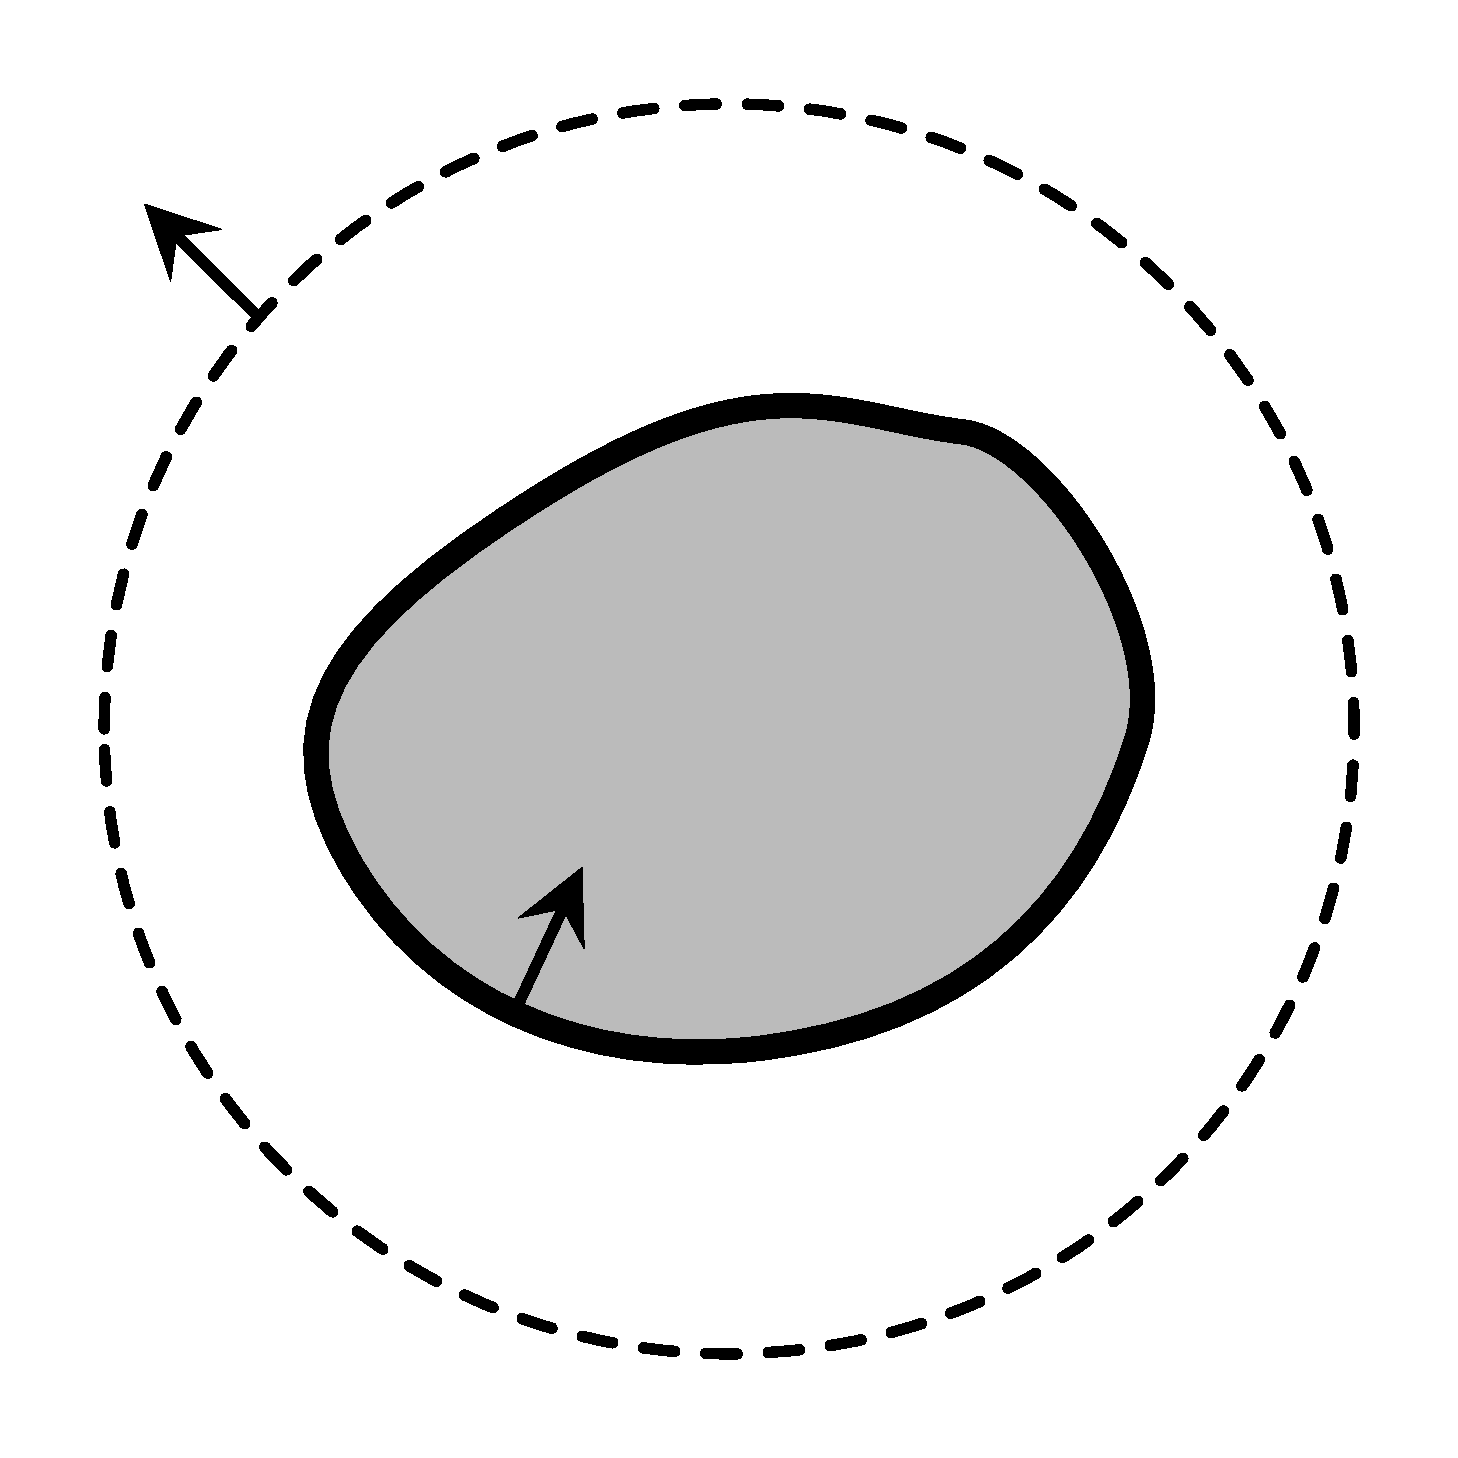
\includegraphics[width=.6\textwidth]{Images/BoundaryIntergral.pdf}};
    \begin{scope}[x={(image.south east)},y={(image.north west)}]
    \begin{scope}[x={(image.south east)},y={(image.north west)}]
        \node at (0.5,0.5) {\Huge $D$};
        \node at (0.41,0.8) {\Huge $S$};
        \node at (0.44,0.39) {\Huge $\bm{n}$};
        \node at (0.15,0.885) {\Huge $\bm{n}$};
    \end{scope}
    \end{scope}
\end{tikzpicture}}
    \caption{A schematic diagram of the volume used in the derivation the boundary integral for Stokes flow}
    \label{fig:SystematicDiagram}
\end{figure}


Suppose we now let $S$ be the volume between the solid body $D$ and a sphere with a radius such that all of $D$ is contained within. We will denote $\partial S$ to be the surface of $S$, note that $\partial S$ is both the surface of the sphere and the surface of the solid body $\partial D$. If we now integrate the above equation over the volume $S$ then we get that
\begin{equation*}
\begin{aligned}
      &\iiint_{S} \left[\frac{1}{8\pi\mu}\frac{\partial}{\partial x_k}(S^\epsilon_{ij}\left(\bm{x}, \bm{y}\right)\sigma_{ik}\left(\bm{x}, \bm{y}\right) - \mu u_i(\bm{x}) T^\epsilon_{ijk}\left(\bm{x}, \bm{y}\right))\right] dV(\bm{x}) \\
      &= \iiint_{S} u_j(\bm{x})\phi_\epsilon(\bm{x}-\bm{y}) dV(\bm{x}).
\end{aligned}
\end{equation*}
Using the divergence theorem on the left-hand side of the equation we get that
\begin{equation*}
  \frac{1}{8\pi\mu}\iint_{\partial S} \left[S^\epsilon_{ij}\left(\bm{x}, \bm{y}\right)\sigma_{ik}\left(\bm{x}, \bm{y}\right) - \mu u_i(\bm{x}) T^\epsilon_{ijk}\left(\bm{x}, \bm{y}\right)\right]n_k ds(\bm{x}) = \iiint_{S} u_j\phi_\epsilon(\bm{x}-\bm{y}) dV(\bm{x})
\end{equation*}
where $\bm{n}$ is the outwards facing unit normal vector of $\partial S$. If we consider the limit as the radius of the sphere tends to infinity, we find that the only contributions to the left-hand side come from $\partial D$. We will introduce the traction on the surface of the sphere as $g_{i} = -\sigma_{ik}n_k$ (as the unit normal points into $D$) and obtain
\begin{equation}
\begin{aligned}
    \label{eq:BIE3}
    &\frac{1}{8\pi\mu}\iint_{\partial D} S^\epsilon_{ij}\left(\bm{x}, \bm{y}\right)g_i(\bm{x}) ds(\bm{x}) - \frac{1}{8\pi}\iint_{\partial D} u_i(\bm{x}) T^\epsilon_{ijk}\left(\bm{x}, \bm{y}\right)n_k(\bm{x}) ds(\bm{x}) \\
    &= \iiint_{S} u_j(\bm{x})\phi_\epsilon(\bm{x}-\bm{y}) dV(\bm{x})
\end{aligned}
\end{equation}
Considering the fluid inside of the solid body $D$ we realise that the velocity must satisfy the zero-deformation condition
\begin{equation*}
  \frac{\partial u_i}{\partial k} + \frac{\partial u_k}{\partial i} = 0
\end{equation*}
This gives us that $\sigma_{ik} = -p\delta_{ik}$ inside of $D$ and as such we obtain that for each $j=1,2,3$
\begin{equation*}
  \iiint_{D} \frac{\partial}{\partial x_k}\left[S^\epsilon_{ij}\left(\bm{x}, \bm{y}\right)\sigma_{ik}\left(\bm{x}, \bm{y}\right)\right]dV(\bm{x}) = -p\iiint_{D} \frac{\partial}{\partial x_k}\left[S^\epsilon_{kj}\left(\bm{x}, \bm{y}\right)\right]dV(\bm{x}) = 0
\end{equation*}
from the incompressibility condition \cref{eq:regcondition2}. If we now integrate \cref{eq:reciprocalrelation} over the volume $D$ instead of $S$ and use the above integral, we have that given $p \neq 0$
\begin{equation}
\begin{aligned}
    \label{eq:BIE4}
    -\frac{1}{8\pi}\iiint_{D} \frac{\partial}{\partial x_k}\left(u_i(\bm{x})T^\epsilon_{ijk}\left(\bm{x}, \bm{y}\right) \right) dV(\bm{x}) &= \frac{1}{8\pi}\iint_{\partial D} u_i(\bm{x})T^\epsilon_{ijk}\left(\bm{x}, \bm{y}\right)n_k(\bm{x}) ds(\bm{x})\\
    &= \iiint_D u_j(\bm{x}) \phi^\epsilon(\bm{x}-\bm{y}) dV(\bm{x}).
\end{aligned}
\end{equation}
We again have used the divergence theorem to convert the volume integral to a surface integral with $n_k$ being the unit normal pointing into $D$. Observing that the sum over \cref{eq:BIE3,eq:BIE4} will give us the integral over $\mathbb{R}^{3}$ and, using the fact that the velocity is continuous on the boundary $\partial D$ we determine that final boundary integral equation is
\begin{equation}
  \label{eq:BIE5}
    \iiint_{\mathbb{R}^{3}} u_{j}(\bm{x}) \phi^{\epsilon}\left(\bm{x}-\bm{y}\right) d V(\bm{x})=-\frac{1}{8 \pi \mu} \iint_{\partial D} S_{i j}^{\epsilon}\left(\bm{x}, \bm{y}\right) g_{i}(\bm{x}) d s(\bm{x}).
\end{equation}
As the traction $\bm{g}$ denotes the traction exerted by the fluid on the body it must have the opposite sign to the stokeslet traction $\bm{f}$ and as such $\bm{f} = -\bm{g}$ where $\bm{f}$ denotes the force per unit area acting on the fluid. To use \cref{eq:BIE5} we need to have an explicit equation for $\bm{u}(\bm{x})$, as such we need to remove the integral and the cutoff function from the left hand side of \cref{eq:BIE5}, we do this though the approximation that $\int_{\mathbb{R}^{3}} u_{j}(\bm{x}) \phi^{\epsilon}\left(\bm{x}-\bm{y}\right) d V(\bm{x}) \approx u_j(\bm{y})$. By taking the approximation as exact we write that 
\begin{equation}
    u_j(\bm{y}) = \frac{1}{8 \pi \mu} \iint_{\partial D} S_{i j}^{\epsilon}\left(\bm{x}, \bm{y}\right) f_{i}(\bm{x}) d s(\bm{x})
\end{equation}
By using the fact that $S_{i j}^{\epsilon}\left(\bm{x}, \bm{y}\right) = S_{j i}^{\epsilon}\left(\bm{y}, \bm{x}\right)$ we can write \cref{eq:BIE5} as 
\begin{equation}
  \label{eq:BIE}
    u(\bm{x})_i=\frac{1}{8 \pi \mu} \iint_{\partial D} S_{i j}^{\epsilon}\left(\bm{x}, \bm{y}\right) f_{j}(\bm{y}) d s(\bm{y})
\end{equation}
The analysis of this error for our particular cutoff function can be see in \cite{Cortez2005} and is found to be of order $\mathcal{O}(\epsilon)$ close to the boundary and $\mathcal{O}(\epsilon^2)$ away from the boundary.

The analytical computation of \cref{eq:BIE} is possible for certain cases allowing for the computation of the fluid velocity given prescribed body forces on the fluid, however, they are often hard or impossible to do by hand. In this case we consider the numerical integration of such problems. By approximating the boundary integral equation with a quadrature rule we obtain a formula for the velocity of the fluid at a point $\bm{y}$. To do this we consider the integral on the right-hand side of \cref{eq:BIE} as the sum over $N$ stokeslets located on the surface of $D$. 
\begin{equation}
\label{eq:Stokesletsum}
    u_{i}\left(\bm{x}\right)=\frac{1}{8 \pi \mu} \sum_{n=1}^{N} \sum_{i=1}^{3} S_{i j}^{\epsilon}\left(\bm{x}, {\bm{y}}_{n}\right) {f}_{j}({\bm{y}}_{n}) A_{n}
\end{equation}
where ${f}_{i}({\bm{y}}_n)$ is the $i$th component of the force on the fluid at the point ${\bm{y}}_n$ and $A_n$ is the corresponding quadrature weight of the $n$th stokeslet.

The discretisation of the integral in \cref{eq:BIE} introduced a discretisation error of $\mathcal{O}(h)$ where $h$ is the average spacing between quadrature points and also a quadrature error which is also dependent on $\epsilon$. Analysis done by Cortez, Fauci and Medovikov \cite{Cortez2005} estimated the quadrature error introduced by this method to be $\mathcal{O}(h^2\epsilon^{-3})$ although more recently analysis by Gallagher, Choudhuri and Smith \cite{Gallagher2019SharpEquation} refined this estimate to $\mathcal{O}(h^2\epsilon^{-1}) + \mathcal{O}(P\epsilon^{-1/P} h^{1-P})$ for any integer $P>3$.

\subsection{Resistance Problem} \label{sec:resistance}
As \cref{eq:Stokesletsum} can be used to calculate the velocity at any point in the fluid $\bm{x}$. By forming a set of collocation points $\{\bm{x}_m\}$ for $m=1,...,M$ we form a dense system of $3M$ equations which calculate the velocity at all points in $\{\bm{x}_m\}$. 
A common issue in Stokes flow is the resistance problem, where the force distribution, and hence total force and moment, on a body is calculated from a prescribed rigid body motion. By prescribing velocities at each point $\{\bm{x}_m\}$ we form a system of $3M$ equations with $3N$ unknowns $F_j(\bm{y}_n) := f_j(\bm{y}_n)A_n$. If $M \neq N$ we either under prescribe or over prescribe the system of equation, so we often choose to place both the collocation and quadrature points at the same set of positions, we will  refer to this as the Nyström discretisation \cite{Nystrom1930UberRandwertaufgaben}. For each of the rigid body motion modes, unit velocity translation along each axis and unit angular velocity rotation about each axis, are calculated we can form the grand resistance matrix $\mathcal{R}$ \cite{Pozrikidis1992BoundaryFlow}. By the linearity of the Stokes equation, $\mathcal{R}$ relates the force $F$ and moment $M$ to the velocity $U$ and angular velocity $V$ for any rigid body motion. 
\begin{equation}
\arraycolsep=1pt\def\arraystretch{1.2}
\left(
\begin{array}{c}
\boldsymbol{F} \\
\boldsymbol{M}
\end{array}\right)=\underbrace{\left(\begin{array}{cc}
A_{F U} & A_{F \Omega} \\
A_{M U} & A_{M \Omega}
\end{array}\right)}_{\mathcal{R}}\left(\begin{array}{c}
\boldsymbol{U} \\
\boldsymbol{\Omega}
\end{array}\right) .
\label{eq:GrandResistance}
\end{equation}
 For example, Stokes Law gives us that the grand resistance matrix for a sphere of radius $r$ centred at the origin is
 \begin{equation}
\arraycolsep=1pt\def\arraystretch{1.2}
\mathcal{R}=\left(\begin{array}{cc}
6\pi\mu r I & 0 \\
0 & 8\pi\mu r^3 I
\end{array}\right)
\label{eq:sphereres}
\end{equation}
where $I$ is the $3\times 3$ identity matrix and $0$ is a $3\times 3$ matrix of zeros. The formulation and computation of these systems promote the use of formulating the problem [does not make sense] in terms of a matrix-vector product where we can make use of highly optimised BLAS (Basic Linear Algebra Subprograms) and LAPACK (Linear Algebra PACKage) packages over direct computations in the code. This allows for the software to use the latest in hardware and software optimisations such as improved multicore algorithms and use across multiple types of hardware with no changes to the higher-level code.

\subsection{Matrix formulation}
The computation of \cref{eq:Stokesletsum} for a set of collocation points $\{\bm{x}_m\}$  for $m = 1,...,M$ can be viewed as the product of a dense $3M \times 3N$ matrix with a $3N \times 1$ column vector where $M$ is the number of collocation points and $N$ the number of stokeslet points. By taking the Nyström discretisation where we choose $\{\bm{x}_m\} = \{\bm{y}_n\}$ the stokeslet matrix therefore becomes a $3N \times 3N$ matrix where the velocity can be calculated from a set of prescribed traction [word missing?] $\{\bm{F}(\bm{x}_n)\}$. 
\begin{equation}
\label{eq:Nystrom}
    u_{i}\left(\bm{x}_m\right)=\frac{1}{8 \pi \mu} \sum_{n=1}^{N} \sum_{i=1}^{3} S_{i j}^{\epsilon}\left(\bm{x}_m, {\bm{x}}_{n}\right) {F}_{j}({\bm{x}}_{n})
\end{equation}
where $n=1,\dots,N$, $m=1,\dots,N$ and $j=1,2,3$. The computation of this matrix-vector product can be written as 
\begin{equation}
\label{eq:matrixvectorproduct}
    \underline{U} = A \underline{F}
\end{equation}
where $\underline{U}$ is a $3N \times 1$ column vector, $A$ is a $3N \times 3N$ matrix and $\underline{F}$ is a $3N \times 1$. To form an equation of this form we choose to write 
\small
\begin{equation*}
    \underline{U} = [u_1({\bm{x}}_{1}), \; u_2({\bm{x}}_{1}), \; u_3({\bm{x}}_{1}), \; u_1({\bm{x}}_{2}), \; u_2({\bm{x}}_{2}), \; u_3({\bm{x}}_{2}), \; \dots \; u_1({\bm{x}}_{M}), \; u_2({\bm{x}}_{M}), \; u_3({\bm{x}}_{N})]^{T}u
\end{equation*}
\normalsize
and 
\small
\begin{equation*}
    \underline{F} = [{f}_{1}({\bm{x}}_{1})A_1, \; {f}_{2}({\bm{x}}_{1})A_1, \; {f}_{3}({\bm{x}}_{1})A_1,\; \dots \; {f}_{1}({\bm{x}}_{N})A_N, \; {f}_{2}({\bm{x}}_{N})A_N, \; f_{3}({\bm{x}}_{N})A_N]^{T}
\end{equation*}
\normalsize
This gives the form of A as 
\small
\begin{equation}
A = 
\begingroup
\setlength\arraycolsep{1pt}
\begin{bmatrix}
S^{\epsilon}_{11}(\bm{x}_1,{\bm{x}}_1) & S^{\epsilon}_{12}(\bm{x}_1,{\bm{x}}_1) & S^{\epsilon}_{13}(\bm{x}_1,{\bm{x}}_1) & \dots & S^{\epsilon}_{11}(\bm{x}_N,{\bm{x}}_1) & S^{\epsilon}_{13}(\bm{x}_N,{\bm{x}}_1) & S^{\epsilon}_{13}(\bm{x}_N,{\bm{x}}_1)\\
S^{\epsilon}_{21}(\bm{x}_1,{\bm{x}}_1) & S^{\epsilon}_{22}(\bm{x}_1,{\bm{x}}_1) & S^{\epsilon}_{23}(\bm{x}_1,{\bm{x}}_1) & \dots & S^{\epsilon}_{21}(\bm{x}_N,{\bm{x}}_1) & S^{\epsilon}_{22}(\bm{x}_N,{\bm{x}}_1) & S^{\epsilon}_{23}(\bm{x}_N,{\bm{x}}_1)\\
S^{\epsilon}_{31}(\bm{x}_1,{\bm{x}}_1) & S^{\epsilon}_{32}(\bm{x}_1,{\bm{x}}_1) & S^{\epsilon}_{33}(\bm{x}_1,{\bm{x}}_1) & \dots & S^{\epsilon}_{31}(\bm{x}_N,{\bm{x}}_1) & S^{\epsilon}_{32}(\bm{x}_N,{\bm{x}}_1) & S^{\epsilon}_{33}(\bm{x}_N,{\bm{x}}_1)\\
\vdots & \vdots & \vdots & \ddots & \vdots & \vdots & \vdots \\
S^{\epsilon}_{11}(\bm{x}_1,{\bm{x}}_N) & S^{\epsilon}_{12}(\bm{x}_1,{\bm{x}}_N) & S^{\epsilon}_{13}(\bm{x}_1,{\bm{x}}_N) & \dots & S^{\epsilon}_{11}(\bm{x}_N,{\bm{x}}_N) & S^{\epsilon}_{12}(\bm{x}_N,{\bm{x}}_N) & S^{\epsilon}_{13}(\bm{x}_N,{\bm{x}}_N)  \\
S^{\epsilon}_{21}(\bm{x}_1,{\bm{x}}_N) & S^{\epsilon}_{22}(\bm{x}_1,{\bm{x}}_N) & S^{\epsilon}_{23}(\bm{x}_1,{\bm{x}}_N) & \dots & S^{\epsilon}_{21}(\bm{x}_N,{\bm{x}}_N) & S^{\epsilon}_{22}(\bm{x}_N,{\bm{x}}_N) & S^{\epsilon}_{23}(\bm{x}_N,{\bm{x}}_N) \\
S^{\epsilon}_{31}(\bm{x}_1,{\bm{x}}_N) & S^{\epsilon}_{32}(\bm{x}_1,{\bm{x}}_N) & S^{\epsilon}_{33}(\bm{x}_1,{\bm{x}}_N) & \dots & S^{\epsilon}_{31}(\bm{x}_N,{\bm{x}}_N) & S^{\epsilon}_{32}(\bm{x}_N,{\bm{x}}_N) & S^{\epsilon}_{33}(\bm{x}_N,{\bm{x}}_N) \\
\end{bmatrix}
\endgroup
\label{eq:StokeletMatrix}
\end{equation}
\normalsize
We do note that this choice in the structure of $U$ and $F$ is not unique and other literature may use different arrangements however they will all produce the same results. The computation of the velocities at the set of points $\{\bm{x}_n\}$ through the direct computation of the full matrix-vector product as the direct product [does not make sense?]. Assembly of the stokeslet matrix requires $9N^2$ function evaluations followed by $\mathcal{O}(N^2)$ operations to compute the vector product. The formulation of the direct product also allows for easy application to resistance problem where $\underline{F} = A^{-1} \underline{U}$, this problem can either be solved through the inversion of the matrix $A$ or, in our implementation, the use of MATLAB's mldivide ($\backslash$) function which both take $\mathcal{O}(N^3)$ operations to compute the solution. For larger systems where the use of mldivide becomes too computationally costly, either from time or memory, the solution can be solved using the Generalized Minimal RESidual (GMRES) method (See \cref{appendix:GMRES}) \cite{Saad1986GMRES:Systems,Elman2005FiniteDynamics}. GMRES can perform the inverse in at worst $\mathcal{O}(N^3)$ however [???] will more often converge to a solution with a small relative residual error in significantly fewer iterations, particularly when an appropriate preconditioner is used.
\FloatBarrier
\section{\texorpdfstring{$N$-body Problems}{N-body Problems}} \label{sec:Nbody}

Under the framework of the method of regularised stokeslets, using the standard boundary integral method, the evaluation of velocities at $N$ locations in this fluid caused by $N$ force points boils down to an $N$-body problem where if computed exactly through the use of the direct product (eq.~\ref{eq:matrixvectorproduct}) requires $\mathcal{O}(N^2)$ calculations. For a large number of particles, the computation time quickly becomes prohibitive due to rapid growth in the number of operations as the number of particles increases. With the rise of more powerful computers, and the need to compute problems with larger number of interactions, fast algorithms for the summation of particle to particle interactions have been developed which aim to reduce the number of calculations needed to solve problems. 

$N$-body problems of the form
\begin{equation*}
    \bm{u}(\bm{x}_i) = \sum_{n=1}^N \Phi(\bm{x}_n,{\bm{x}}_n){\bm{f}}_n
\end{equation*}
where $\Phi$ is the Green's function associated with the underlying partial differential equation governing the dynamics of the system arise in many problems from electrostatics \cite{Beatson,Tornberg2008}, heat conduction \cite{Greengard1990APotentials}, Stokes flow \cite{Cortez2015,Tornberg2008} and stellar dynamics \cite{Dehnen2014ADynamics}. Most methods of fast summation utilise tree based grouping of the particles in order to form clusters of particles in which the particle to particles can be computed quickly and efficiently. 

In this section we will explore the development of tree based algorithms for the fast summation of $N$-body problems, in particular the Barnes-Hut method \cite{Barnes1986} \cref{subsec:BarnesHut} which provides an easily implemented method for solving $N$-body systems and an $\mathcal{O}(N\log N)$ complexity for the summation. From the Barnes-Hut method we will explore how Greengard and Rokhlin \cite{1988The0-262-7110-X.,Rokhlin1985RapidTheory,Greengard1987ASimulations} adapted the Barnes-Hut method to create analytically correct results while still retaining $\mathcal{O}(N\log N)$ complexity by using multipole expansions (\cref{subsec:ExactNlogN}). The use of multipole expansion was later expanded by Greengard, Rokhlin and Beatson \cite{Beatson,Greengard1987ASimulations} to create an analytically correct algorithm with complexity $\mathcal{O}(N)$ called the Fast Mutlipole Method (FMM). We will explore briefly how these multipole expansion can be used in the 2D case of the Coulombs potential in order to illustrate the ideas behind the algorithm. However, due to the need to form factorisations of the kernel which are not easily obtained of the method of regularised stokeslets, although can be obtained for singular Stokelet and Stresslet kernels \cref{eq:singularsolutions} \cite{Tornberg2008}, we need to consider a kernel independent method. In \cref{sec:KIFMM} we will review the Kernel Independent Fast Multipole Method (KIFMM) created by Ying, Biros and Zorin \cite{Ying2004}, and how it can be adapted for use with the method of regularised stokeslets. 

We will also consider in \cref{sec:NEAREST} an adaption to the Nyström method based on nearest neighbour interpolation which reduces the overall size of the system and decouples $\epsilon$ from the force quadrature spacing $h$. This method provides a easy method to reduce the overall number of particles which need to be considered when solving problems such as resistance problems (\cref{sec:resistance}) or swimming problems (\cref{sec:swimming}).
We will also consider a hybrid implentation of the KIFMM and NEAREST method and explore its use in \cref{sec:NumericalSims}. Due to the single direction of the computation of FMM algorithms we will also explore how the GMRES algorithm can be used with this hybrid method to solve large swimming problems including the derivations of an appropriate preconditioner.  

\subsection{Barnes-Hut Method} \label{subsec:BarnesHut}
One of the first methods proposed to compute $N$-body systems was that of Barnes and Hut \cite{Barnes1986} and is a tree-based method for the computation of $N$-body simulations. By using a Quadtree in two dimensions \cref{fig:2DDecompostion} or octtree in three dimensions \cref{fig:Decompostionexample} the number of computations needed in the $N$-body problem is reduced to $\mathcal{O}(N\log N)$. Tree-based decomposition uses a tree data structure to `bin' particles in smaller domains in which we can consider particle to particle interactions for particles close to each other and an approximation of the particle for particles further away. 


\subsection{Tree-Based Decomposition} \label{sec:TreeDecomp}

\begin{figure}
    \begin{subfigure}[b]{0.4\textwidth}
        \centering
        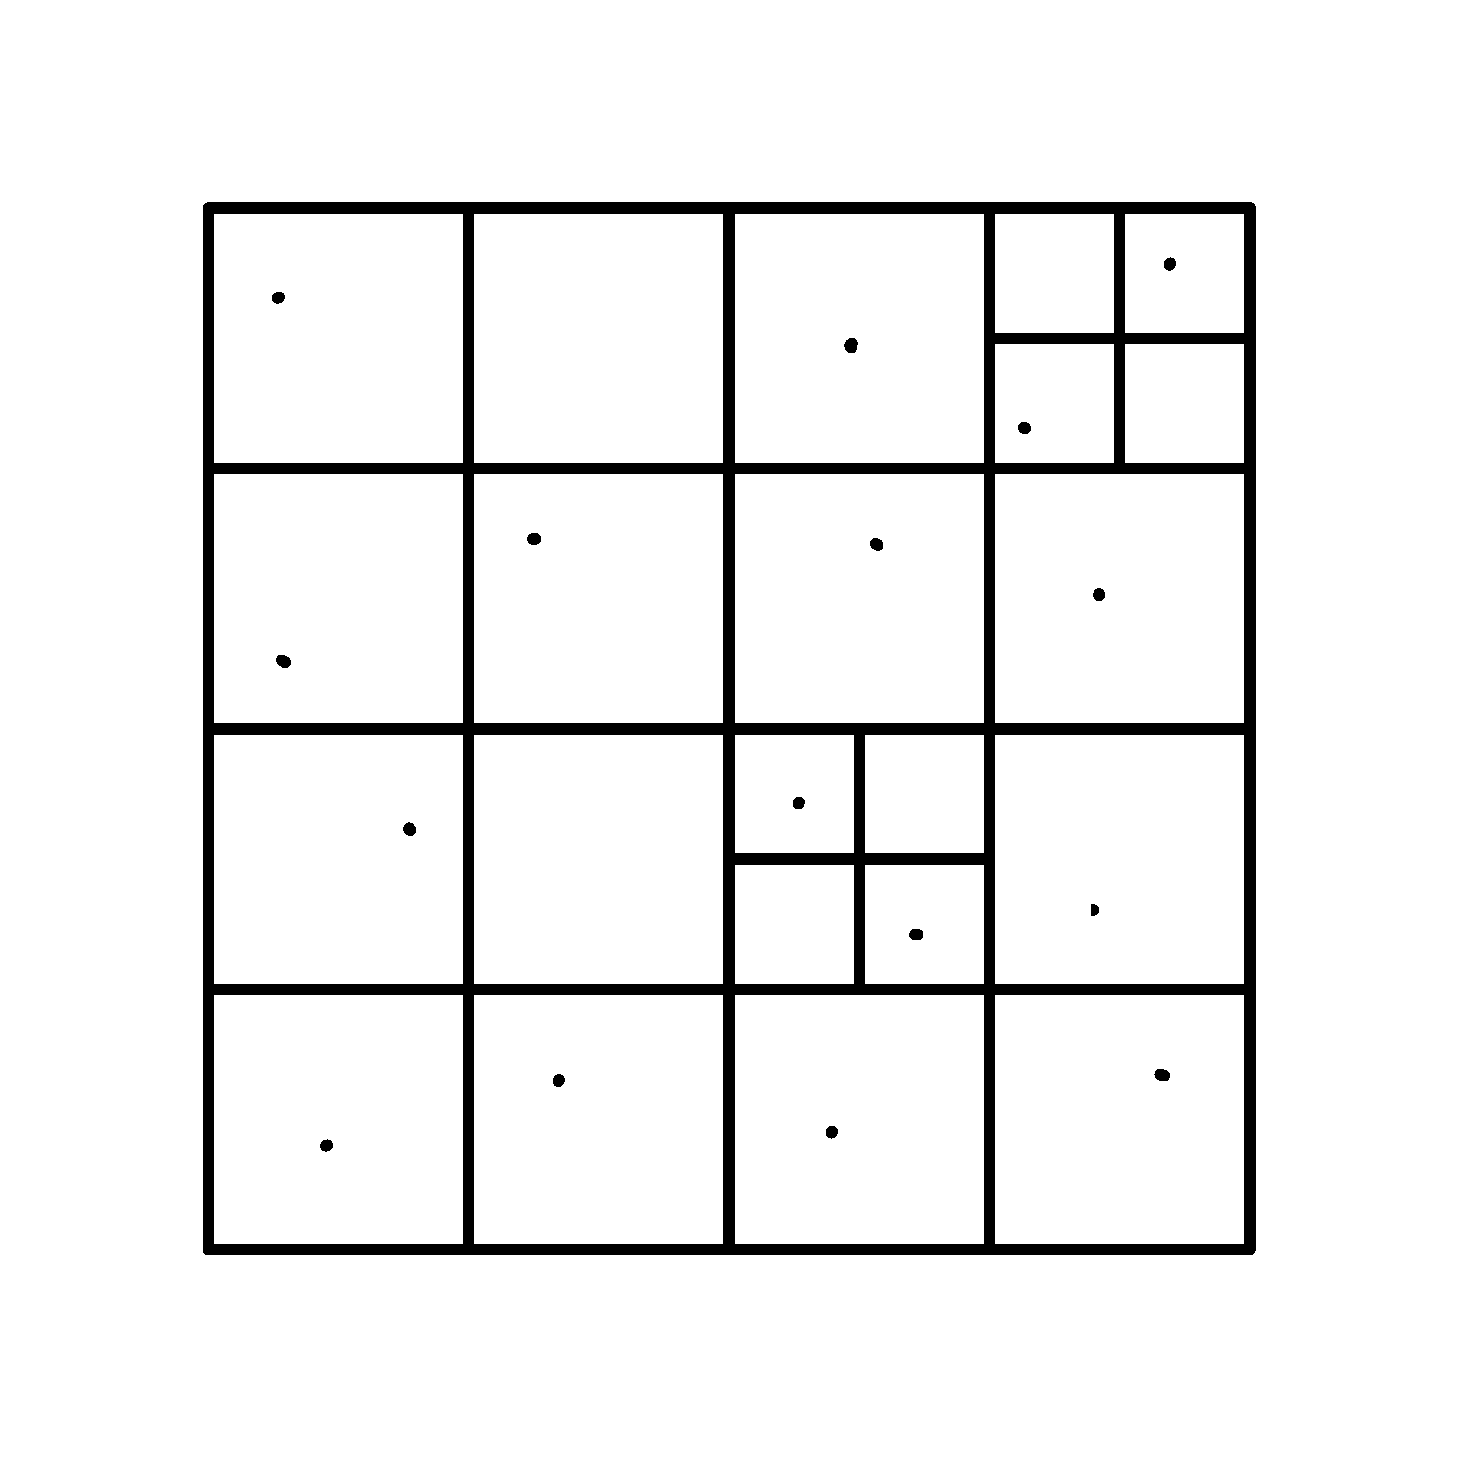
\includegraphics[width=\textwidth]{Images/KIFMM/Decomposition.pdf}
        \caption{\label{fig:2DDecompostion}}
    \end{subfigure}
    \hfill
    \begin{subfigure}[b]{0.4\textwidth}
    \centering
        \resizebox{\linewidth}{!}{% This file was created by matlab2tikz.
%
%The latest updates can be retrieved from
%  http://www.mathworks.com/matlabcentral/fileexchange/22022-matlab2tikz-matlab2tikz
%where you can also make suggestions and rate matlab2tikz.
%
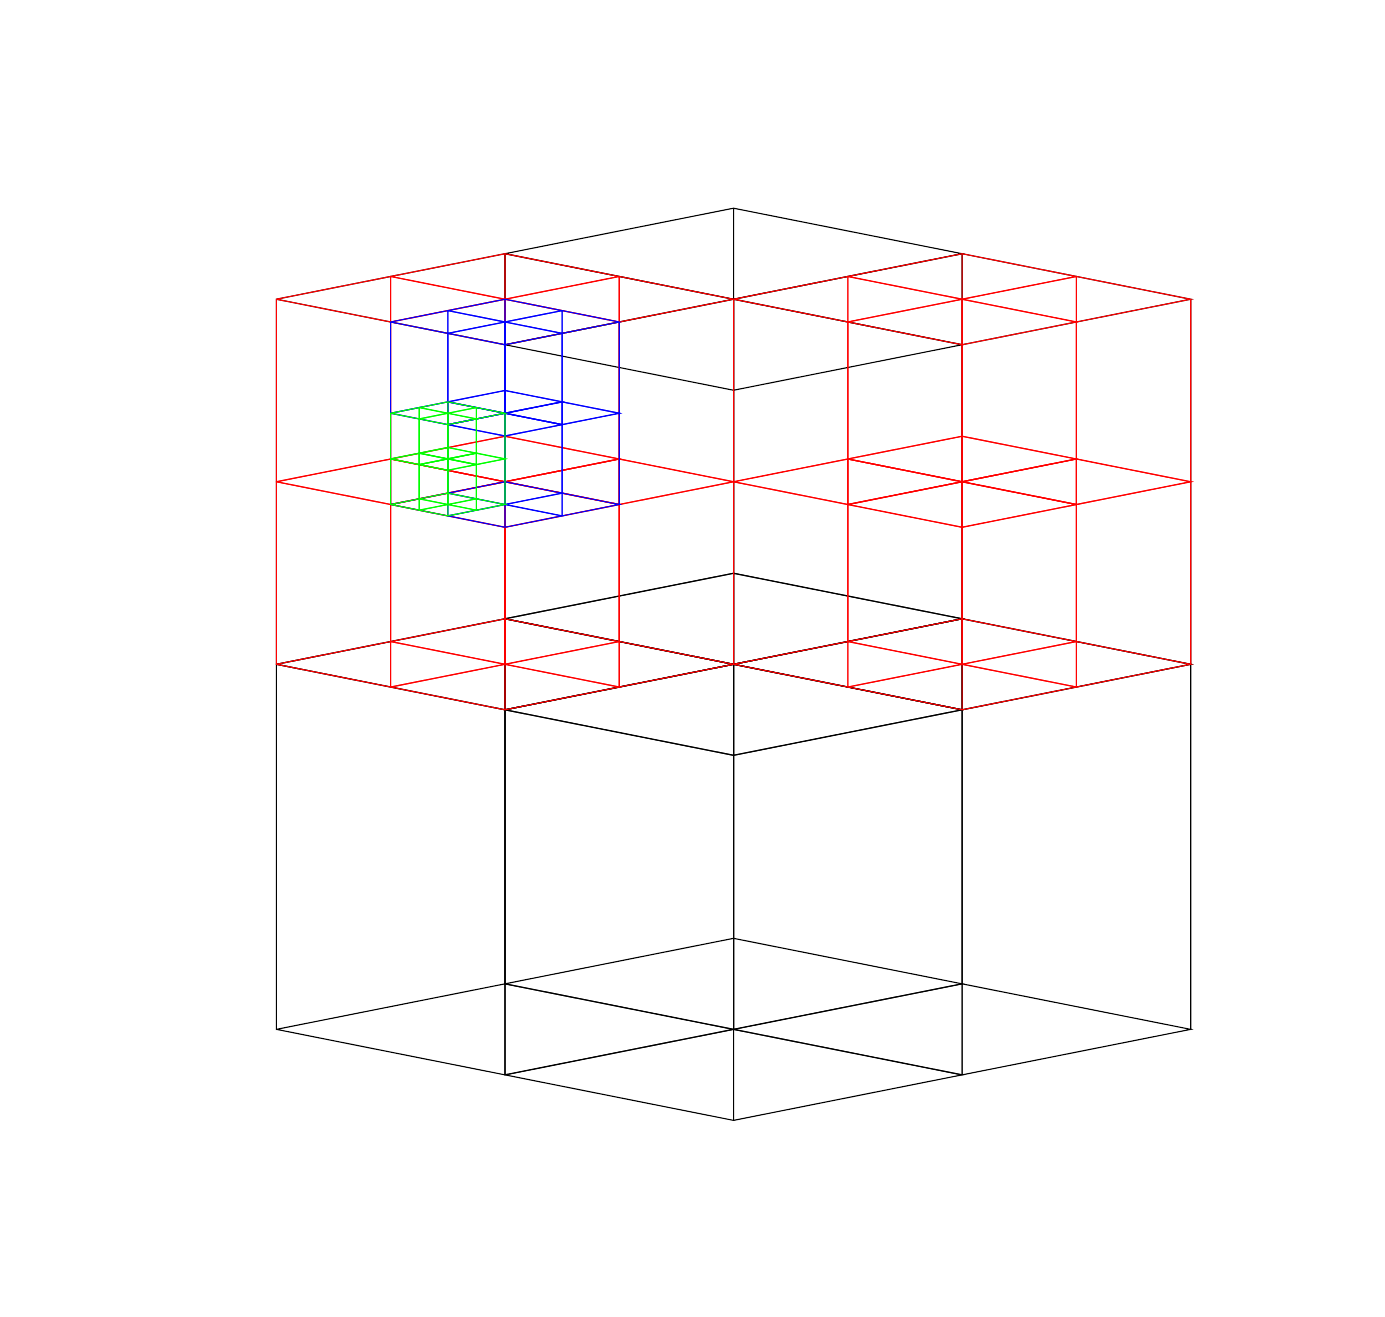
\begin{tikzpicture}

\begin{axis}[%
width=5.151in,
height=5.139in,
at={(0.864in,0.694in)},
scale only axis,
unbounded coords=jump,
xmin=0,
xmax=1,
tick align=outside,
ymin=0,
ymax=1,
zmin=0,
zmax=1,
view={45}{10},
axis line style={draw=none},
ticks=none,
axis x line*=bottom,
axis y line*=left,
axis z line*=left
]
\addplot3 [color=black]
 table[row sep=crcr] {%
0.0737015537421595	0.0737015537421595	0.0737015537421595\\
0.517448266926349	0.0737015537421595	0.0737015537421595\\
0.517448266926349	0.517448266926349	0.0737015537421595\\
0.0737015537421595	0.517448266926349	0.0737015537421595\\
0.0737015537421595	0.0737015537421595	0.0737015537421595\\
0.0737015537421595	0.0737015537421595	0.517448266926349\\
0.517448266926349	0.0737015537421595	0.517448266926349\\
0.517448266926349	0.517448266926349	0.517448266926349\\
0.0737015537421595	0.517448266926349	0.517448266926349\\
0.0737015537421595	0.0737015537421595	0.517448266926349\\
0.0737015537421595	0.0737015537421595	0.0737015537421595\\
nan	nan	nan\\
0.517448266926349	0.0737015537421595	0.0737015537421595\\
0.517448266926349	0.0737015537421595	0.517448266926349\\
nan	nan	nan\\
0.517448266926349	0.517448266926349	0.0737015537421595\\
0.517448266926349	0.517448266926349	0.517448266926349\\
nan	nan	nan\\
0.0737015537421595	0.517448266926349	0.0737015537421595\\
0.0737015537421595	0.517448266926349	0.517448266926349\\
};
 \addplot3 [color=black]
 table[row sep=crcr] {%
0.0737015537421595	0.0737015537421595	0.517448266926349\\
0.517448266926349	0.0737015537421595	0.517448266926349\\
0.517448266926349	0.517448266926349	0.517448266926349\\
0.0737015537421595	0.517448266926349	0.517448266926349\\
0.0737015537421595	0.0737015537421595	0.517448266926349\\
0.0737015537421595	0.0737015537421595	0.961194980110539\\
0.517448266926349	0.0737015537421595	0.961194980110539\\
0.517448266926349	0.517448266926349	0.961194980110539\\
0.0737015537421595	0.517448266926349	0.961194980110539\\
0.0737015537421595	0.0737015537421595	0.961194980110539\\
0.0737015537421595	0.0737015537421595	0.517448266926349\\
nan	nan	nan\\
0.517448266926349	0.0737015537421595	0.517448266926349\\
0.517448266926349	0.0737015537421595	0.961194980110539\\
nan	nan	nan\\
0.517448266926349	0.517448266926349	0.517448266926349\\
0.517448266926349	0.517448266926349	0.961194980110539\\
nan	nan	nan\\
0.0737015537421595	0.517448266926349	0.517448266926349\\
0.0737015537421595	0.517448266926349	0.961194980110539\\
};
 \addplot3 [color=black]
 table[row sep=crcr] {%
0.0737015537421595	0.517448266926349	0.0737015537421595\\
0.517448266926349	0.517448266926349	0.0737015537421595\\
0.517448266926349	0.961194980110539	0.0737015537421595\\
0.0737015537421595	0.961194980110539	0.0737015537421595\\
0.0737015537421595	0.517448266926349	0.0737015537421595\\
0.0737015537421595	0.517448266926349	0.517448266926349\\
0.517448266926349	0.517448266926349	0.517448266926349\\
0.517448266926349	0.961194980110539	0.517448266926349\\
0.0737015537421595	0.961194980110539	0.517448266926349\\
0.0737015537421595	0.517448266926349	0.517448266926349\\
0.0737015537421595	0.517448266926349	0.0737015537421595\\
nan	nan	nan\\
0.517448266926349	0.517448266926349	0.0737015537421595\\
0.517448266926349	0.517448266926349	0.517448266926349\\
nan	nan	nan\\
0.517448266926349	0.961194980110539	0.0737015537421595\\
0.517448266926349	0.961194980110539	0.517448266926349\\
nan	nan	nan\\
0.0737015537421595	0.961194980110539	0.0737015537421595\\
0.0737015537421595	0.961194980110539	0.517448266926349\\
};
 \addplot3 [color=black]
 table[row sep=crcr] {%
0.0737015537421595	0.517448266926349	0.517448266926349\\
0.517448266926349	0.517448266926349	0.517448266926349\\
0.517448266926349	0.961194980110539	0.517448266926349\\
0.0737015537421595	0.961194980110539	0.517448266926349\\
0.0737015537421595	0.517448266926349	0.517448266926349\\
0.0737015537421595	0.517448266926349	0.961194980110539\\
0.517448266926349	0.517448266926349	0.961194980110539\\
0.517448266926349	0.961194980110539	0.961194980110539\\
0.0737015537421595	0.961194980110539	0.961194980110539\\
0.0737015537421595	0.517448266926349	0.961194980110539\\
0.0737015537421595	0.517448266926349	0.517448266926349\\
nan	nan	nan\\
0.517448266926349	0.517448266926349	0.517448266926349\\
0.517448266926349	0.517448266926349	0.961194980110539\\
nan	nan	nan\\
0.517448266926349	0.961194980110539	0.517448266926349\\
0.517448266926349	0.961194980110539	0.961194980110539\\
nan	nan	nan\\
0.0737015537421595	0.961194980110539	0.517448266926349\\
0.0737015537421595	0.961194980110539	0.961194980110539\\
};
 \addplot3 [color=black]
 table[row sep=crcr] {%
0.517448266926349	0.0737015537421595	0.0737015537421595\\
0.961194980110539	0.0737015537421595	0.0737015537421595\\
0.961194980110539	0.517448266926349	0.0737015537421595\\
0.517448266926349	0.517448266926349	0.0737015537421595\\
0.517448266926349	0.0737015537421595	0.0737015537421595\\
0.517448266926349	0.0737015537421595	0.517448266926349\\
0.961194980110539	0.0737015537421595	0.517448266926349\\
0.961194980110539	0.517448266926349	0.517448266926349\\
0.517448266926349	0.517448266926349	0.517448266926349\\
0.517448266926349	0.0737015537421595	0.517448266926349\\
0.517448266926349	0.0737015537421595	0.0737015537421595\\
nan	nan	nan\\
0.961194980110539	0.0737015537421595	0.0737015537421595\\
0.961194980110539	0.0737015537421595	0.517448266926349\\
nan	nan	nan\\
0.961194980110539	0.517448266926349	0.0737015537421595\\
0.961194980110539	0.517448266926349	0.517448266926349\\
nan	nan	nan\\
0.517448266926349	0.517448266926349	0.0737015537421595\\
0.517448266926349	0.517448266926349	0.517448266926349\\
};
 \addplot3 [color=black]
 table[row sep=crcr] {%
0.517448266926349	0.0737015537421595	0.517448266926349\\
0.961194980110539	0.0737015537421595	0.517448266926349\\
0.961194980110539	0.517448266926349	0.517448266926349\\
0.517448266926349	0.517448266926349	0.517448266926349\\
0.517448266926349	0.0737015537421595	0.517448266926349\\
0.517448266926349	0.0737015537421595	0.961194980110539\\
0.961194980110539	0.0737015537421595	0.961194980110539\\
0.961194980110539	0.517448266926349	0.961194980110539\\
0.517448266926349	0.517448266926349	0.961194980110539\\
0.517448266926349	0.0737015537421595	0.961194980110539\\
0.517448266926349	0.0737015537421595	0.517448266926349\\
nan	nan	nan\\
0.961194980110539	0.0737015537421595	0.517448266926349\\
0.961194980110539	0.0737015537421595	0.961194980110539\\
nan	nan	nan\\
0.961194980110539	0.517448266926349	0.517448266926349\\
0.961194980110539	0.517448266926349	0.961194980110539\\
nan	nan	nan\\
0.517448266926349	0.517448266926349	0.517448266926349\\
0.517448266926349	0.517448266926349	0.961194980110539\\
};
 \addplot3 [color=black]
 table[row sep=crcr] {%
0.517448266926349	0.517448266926349	0.0737015537421595\\
0.961194980110539	0.517448266926349	0.0737015537421595\\
0.961194980110539	0.961194980110539	0.0737015537421595\\
0.517448266926349	0.961194980110539	0.0737015537421595\\
0.517448266926349	0.517448266926349	0.0737015537421595\\
0.517448266926349	0.517448266926349	0.517448266926349\\
0.961194980110539	0.517448266926349	0.517448266926349\\
0.961194980110539	0.961194980110539	0.517448266926349\\
0.517448266926349	0.961194980110539	0.517448266926349\\
0.517448266926349	0.517448266926349	0.517448266926349\\
0.517448266926349	0.517448266926349	0.0737015537421595\\
nan	nan	nan\\
0.961194980110539	0.517448266926349	0.0737015537421595\\
0.961194980110539	0.517448266926349	0.517448266926349\\
nan	nan	nan\\
0.961194980110539	0.961194980110539	0.0737015537421595\\
0.961194980110539	0.961194980110539	0.517448266926349\\
nan	nan	nan\\
0.517448266926349	0.961194980110539	0.0737015537421595\\
0.517448266926349	0.961194980110539	0.517448266926349\\
};
 \addplot3 [color=black]
 table[row sep=crcr] {%
0.517448266926349	0.517448266926349	0.517448266926349\\
0.961194980110539	0.517448266926349	0.517448266926349\\
0.961194980110539	0.961194980110539	0.517448266926349\\
0.517448266926349	0.961194980110539	0.517448266926349\\
0.517448266926349	0.517448266926349	0.517448266926349\\
0.517448266926349	0.517448266926349	0.961194980110539\\
0.961194980110539	0.517448266926349	0.961194980110539\\
0.961194980110539	0.961194980110539	0.961194980110539\\
0.517448266926349	0.961194980110539	0.961194980110539\\
0.517448266926349	0.517448266926349	0.961194980110539\\
0.517448266926349	0.517448266926349	0.517448266926349\\
nan	nan	nan\\
0.961194980110539	0.517448266926349	0.517448266926349\\
0.961194980110539	0.517448266926349	0.961194980110539\\
nan	nan	nan\\
0.961194980110539	0.961194980110539	0.517448266926349\\
0.961194980110539	0.961194980110539	0.961194980110539\\
nan	nan	nan\\
0.517448266926349	0.961194980110539	0.517448266926349\\
0.517448266926349	0.961194980110539	0.961194980110539\\
};
 \addplot3 [color=red]
 table[row sep=crcr] {%
0.0737015537421595	0.0737015537421595	0.517448266926349\\
0.295574910334254	0.0737015537421595	0.517448266926349\\
0.295574910334254	0.295574910334254	0.517448266926349\\
0.0737015537421595	0.295574910334254	0.517448266926349\\
0.0737015537421595	0.0737015537421595	0.517448266926349\\
0.0737015537421595	0.0737015537421595	0.739321623518444\\
0.295574910334254	0.0737015537421595	0.739321623518444\\
0.295574910334254	0.295574910334254	0.739321623518444\\
0.0737015537421595	0.295574910334254	0.739321623518444\\
0.0737015537421595	0.0737015537421595	0.739321623518444\\
0.0737015537421595	0.0737015537421595	0.517448266926349\\
nan	nan	nan\\
0.295574910334254	0.0737015537421595	0.517448266926349\\
0.295574910334254	0.0737015537421595	0.739321623518444\\
nan	nan	nan\\
0.295574910334254	0.295574910334254	0.517448266926349\\
0.295574910334254	0.295574910334254	0.739321623518444\\
nan	nan	nan\\
0.0737015537421595	0.295574910334254	0.517448266926349\\
0.0737015537421595	0.295574910334254	0.739321623518444\\
};
 \addplot3 [color=red]
 table[row sep=crcr] {%
0.0737015537421595	0.0737015537421595	0.739321623518444\\
0.295574910334254	0.0737015537421595	0.739321623518444\\
0.295574910334254	0.295574910334254	0.739321623518444\\
0.0737015537421595	0.295574910334254	0.739321623518444\\
0.0737015537421595	0.0737015537421595	0.739321623518444\\
0.0737015537421595	0.0737015537421595	0.961194980110539\\
0.295574910334254	0.0737015537421595	0.961194980110539\\
0.295574910334254	0.295574910334254	0.961194980110539\\
0.0737015537421595	0.295574910334254	0.961194980110539\\
0.0737015537421595	0.0737015537421595	0.961194980110539\\
0.0737015537421595	0.0737015537421595	0.739321623518444\\
nan	nan	nan\\
0.295574910334254	0.0737015537421595	0.739321623518444\\
0.295574910334254	0.0737015537421595	0.961194980110539\\
nan	nan	nan\\
0.295574910334254	0.295574910334254	0.739321623518444\\
0.295574910334254	0.295574910334254	0.961194980110539\\
nan	nan	nan\\
0.0737015537421595	0.295574910334254	0.739321623518444\\
0.0737015537421595	0.295574910334254	0.961194980110539\\
};
 \addplot3 [color=red]
 table[row sep=crcr] {%
0.0737015537421595	0.295574910334254	0.517448266926349\\
0.295574910334254	0.295574910334254	0.517448266926349\\
0.295574910334254	0.517448266926349	0.517448266926349\\
0.0737015537421595	0.517448266926349	0.517448266926349\\
0.0737015537421595	0.295574910334254	0.517448266926349\\
0.0737015537421595	0.295574910334254	0.739321623518444\\
0.295574910334254	0.295574910334254	0.739321623518444\\
0.295574910334254	0.517448266926349	0.739321623518444\\
0.0737015537421595	0.517448266926349	0.739321623518444\\
0.0737015537421595	0.295574910334254	0.739321623518444\\
0.0737015537421595	0.295574910334254	0.517448266926349\\
nan	nan	nan\\
0.295574910334254	0.295574910334254	0.517448266926349\\
0.295574910334254	0.295574910334254	0.739321623518444\\
nan	nan	nan\\
0.295574910334254	0.517448266926349	0.517448266926349\\
0.295574910334254	0.517448266926349	0.739321623518444\\
nan	nan	nan\\
0.0737015537421595	0.517448266926349	0.517448266926349\\
0.0737015537421595	0.517448266926349	0.739321623518444\\
};
 \addplot3 [color=red]
 table[row sep=crcr] {%
0.0737015537421595	0.295574910334254	0.739321623518444\\
0.295574910334254	0.295574910334254	0.739321623518444\\
0.295574910334254	0.517448266926349	0.739321623518444\\
0.0737015537421595	0.517448266926349	0.739321623518444\\
0.0737015537421595	0.295574910334254	0.739321623518444\\
0.0737015537421595	0.295574910334254	0.961194980110539\\
0.295574910334254	0.295574910334254	0.961194980110539\\
0.295574910334254	0.517448266926349	0.961194980110539\\
0.0737015537421595	0.517448266926349	0.961194980110539\\
0.0737015537421595	0.295574910334254	0.961194980110539\\
0.0737015537421595	0.295574910334254	0.739321623518444\\
nan	nan	nan\\
0.295574910334254	0.295574910334254	0.739321623518444\\
0.295574910334254	0.295574910334254	0.961194980110539\\
nan	nan	nan\\
0.295574910334254	0.517448266926349	0.739321623518444\\
0.295574910334254	0.517448266926349	0.961194980110539\\
nan	nan	nan\\
0.0737015537421595	0.517448266926349	0.739321623518444\\
0.0737015537421595	0.517448266926349	0.961194980110539\\
};
 \addplot3 [color=red]
 table[row sep=crcr] {%
0.295574910334254	0.0737015537421595	0.517448266926349\\
0.517448266926349	0.0737015537421595	0.517448266926349\\
0.517448266926349	0.295574910334254	0.517448266926349\\
0.295574910334254	0.295574910334254	0.517448266926349\\
0.295574910334254	0.0737015537421595	0.517448266926349\\
0.295574910334254	0.0737015537421595	0.739321623518444\\
0.517448266926349	0.0737015537421595	0.739321623518444\\
0.517448266926349	0.295574910334254	0.739321623518444\\
0.295574910334254	0.295574910334254	0.739321623518444\\
0.295574910334254	0.0737015537421595	0.739321623518444\\
0.295574910334254	0.0737015537421595	0.517448266926349\\
nan	nan	nan\\
0.517448266926349	0.0737015537421595	0.517448266926349\\
0.517448266926349	0.0737015537421595	0.739321623518444\\
nan	nan	nan\\
0.517448266926349	0.295574910334254	0.517448266926349\\
0.517448266926349	0.295574910334254	0.739321623518444\\
nan	nan	nan\\
0.295574910334254	0.295574910334254	0.517448266926349\\
0.295574910334254	0.295574910334254	0.739321623518444\\
};
 \addplot3 [color=red]
 table[row sep=crcr] {%
0.295574910334254	0.0737015537421595	0.739321623518444\\
0.517448266926349	0.0737015537421595	0.739321623518444\\
0.517448266926349	0.295574910334254	0.739321623518444\\
0.295574910334254	0.295574910334254	0.739321623518444\\
0.295574910334254	0.0737015537421595	0.739321623518444\\
0.295574910334254	0.0737015537421595	0.961194980110539\\
0.517448266926349	0.0737015537421595	0.961194980110539\\
0.517448266926349	0.295574910334254	0.961194980110539\\
0.295574910334254	0.295574910334254	0.961194980110539\\
0.295574910334254	0.0737015537421595	0.961194980110539\\
0.295574910334254	0.0737015537421595	0.739321623518444\\
nan	nan	nan\\
0.517448266926349	0.0737015537421595	0.739321623518444\\
0.517448266926349	0.0737015537421595	0.961194980110539\\
nan	nan	nan\\
0.517448266926349	0.295574910334254	0.739321623518444\\
0.517448266926349	0.295574910334254	0.961194980110539\\
nan	nan	nan\\
0.295574910334254	0.295574910334254	0.739321623518444\\
0.295574910334254	0.295574910334254	0.961194980110539\\
};
 \addplot3 [color=red]
 table[row sep=crcr] {%
0.295574910334254	0.295574910334254	0.517448266926349\\
0.517448266926349	0.295574910334254	0.517448266926349\\
0.517448266926349	0.517448266926349	0.517448266926349\\
0.295574910334254	0.517448266926349	0.517448266926349\\
0.295574910334254	0.295574910334254	0.517448266926349\\
0.295574910334254	0.295574910334254	0.739321623518444\\
0.517448266926349	0.295574910334254	0.739321623518444\\
0.517448266926349	0.517448266926349	0.739321623518444\\
0.295574910334254	0.517448266926349	0.739321623518444\\
0.295574910334254	0.295574910334254	0.739321623518444\\
0.295574910334254	0.295574910334254	0.517448266926349\\
nan	nan	nan\\
0.517448266926349	0.295574910334254	0.517448266926349\\
0.517448266926349	0.295574910334254	0.739321623518444\\
nan	nan	nan\\
0.517448266926349	0.517448266926349	0.517448266926349\\
0.517448266926349	0.517448266926349	0.739321623518444\\
nan	nan	nan\\
0.295574910334254	0.517448266926349	0.517448266926349\\
0.295574910334254	0.517448266926349	0.739321623518444\\
};
 \addplot3 [color=red]
 table[row sep=crcr] {%
0.295574910334254	0.295574910334254	0.739321623518444\\
0.517448266926349	0.295574910334254	0.739321623518444\\
0.517448266926349	0.517448266926349	0.739321623518444\\
0.295574910334254	0.517448266926349	0.739321623518444\\
0.295574910334254	0.295574910334254	0.739321623518444\\
0.295574910334254	0.295574910334254	0.961194980110539\\
0.517448266926349	0.295574910334254	0.961194980110539\\
0.517448266926349	0.517448266926349	0.961194980110539\\
0.295574910334254	0.517448266926349	0.961194980110539\\
0.295574910334254	0.295574910334254	0.961194980110539\\
0.295574910334254	0.295574910334254	0.739321623518444\\
nan	nan	nan\\
0.517448266926349	0.295574910334254	0.739321623518444\\
0.517448266926349	0.295574910334254	0.961194980110539\\
nan	nan	nan\\
0.517448266926349	0.517448266926349	0.739321623518444\\
0.517448266926349	0.517448266926349	0.961194980110539\\
nan	nan	nan\\
0.295574910334254	0.517448266926349	0.739321623518444\\
0.295574910334254	0.517448266926349	0.961194980110539\\
};
 \addplot3 [color=red]
 table[row sep=crcr] {%
0.517448266926349	0.517448266926349	0.517448266926349\\
0.739321623518444	0.517448266926349	0.517448266926349\\
0.739321623518444	0.739321623518444	0.517448266926349\\
0.517448266926349	0.739321623518444	0.517448266926349\\
0.517448266926349	0.517448266926349	0.517448266926349\\
0.517448266926349	0.517448266926349	0.739321623518444\\
0.739321623518444	0.517448266926349	0.739321623518444\\
0.739321623518444	0.739321623518444	0.739321623518444\\
0.517448266926349	0.739321623518444	0.739321623518444\\
0.517448266926349	0.517448266926349	0.739321623518444\\
0.517448266926349	0.517448266926349	0.517448266926349\\
nan	nan	nan\\
0.739321623518444	0.517448266926349	0.517448266926349\\
0.739321623518444	0.517448266926349	0.739321623518444\\
nan	nan	nan\\
0.739321623518444	0.739321623518444	0.517448266926349\\
0.739321623518444	0.739321623518444	0.739321623518444\\
nan	nan	nan\\
0.517448266926349	0.739321623518444	0.517448266926349\\
0.517448266926349	0.739321623518444	0.739321623518444\\
};
 \addplot3 [color=red]
 table[row sep=crcr] {%
0.517448266926349	0.517448266926349	0.739321623518444\\
0.739321623518444	0.517448266926349	0.739321623518444\\
0.739321623518444	0.739321623518444	0.739321623518444\\
0.517448266926349	0.739321623518444	0.739321623518444\\
0.517448266926349	0.517448266926349	0.739321623518444\\
0.517448266926349	0.517448266926349	0.961194980110539\\
0.739321623518444	0.517448266926349	0.961194980110539\\
0.739321623518444	0.739321623518444	0.961194980110539\\
0.517448266926349	0.739321623518444	0.961194980110539\\
0.517448266926349	0.517448266926349	0.961194980110539\\
0.517448266926349	0.517448266926349	0.739321623518444\\
nan	nan	nan\\
0.739321623518444	0.517448266926349	0.739321623518444\\
0.739321623518444	0.517448266926349	0.961194980110539\\
nan	nan	nan\\
0.739321623518444	0.739321623518444	0.739321623518444\\
0.739321623518444	0.739321623518444	0.961194980110539\\
nan	nan	nan\\
0.517448266926349	0.739321623518444	0.739321623518444\\
0.517448266926349	0.739321623518444	0.961194980110539\\
};
 \addplot3 [color=red]
 table[row sep=crcr] {%
0.517448266926349	0.739321623518444	0.517448266926349\\
0.739321623518444	0.739321623518444	0.517448266926349\\
0.739321623518444	0.961194980110539	0.517448266926349\\
0.517448266926349	0.961194980110539	0.517448266926349\\
0.517448266926349	0.739321623518444	0.517448266926349\\
0.517448266926349	0.739321623518444	0.739321623518444\\
0.739321623518444	0.739321623518444	0.739321623518444\\
0.739321623518444	0.961194980110539	0.739321623518444\\
0.517448266926349	0.961194980110539	0.739321623518444\\
0.517448266926349	0.739321623518444	0.739321623518444\\
0.517448266926349	0.739321623518444	0.517448266926349\\
nan	nan	nan\\
0.739321623518444	0.739321623518444	0.517448266926349\\
0.739321623518444	0.739321623518444	0.739321623518444\\
nan	nan	nan\\
0.739321623518444	0.961194980110539	0.517448266926349\\
0.739321623518444	0.961194980110539	0.739321623518444\\
nan	nan	nan\\
0.517448266926349	0.961194980110539	0.517448266926349\\
0.517448266926349	0.961194980110539	0.739321623518444\\
};
 \addplot3 [color=red]
 table[row sep=crcr] {%
0.517448266926349	0.739321623518444	0.739321623518444\\
0.739321623518444	0.739321623518444	0.739321623518444\\
0.739321623518444	0.961194980110539	0.739321623518444\\
0.517448266926349	0.961194980110539	0.739321623518444\\
0.517448266926349	0.739321623518444	0.739321623518444\\
0.517448266926349	0.739321623518444	0.961194980110539\\
0.739321623518444	0.739321623518444	0.961194980110539\\
0.739321623518444	0.961194980110539	0.961194980110539\\
0.517448266926349	0.961194980110539	0.961194980110539\\
0.517448266926349	0.739321623518444	0.961194980110539\\
0.517448266926349	0.739321623518444	0.739321623518444\\
nan	nan	nan\\
0.739321623518444	0.739321623518444	0.739321623518444\\
0.739321623518444	0.739321623518444	0.961194980110539\\
nan	nan	nan\\
0.739321623518444	0.961194980110539	0.739321623518444\\
0.739321623518444	0.961194980110539	0.961194980110539\\
nan	nan	nan\\
0.517448266926349	0.961194980110539	0.739321623518444\\
0.517448266926349	0.961194980110539	0.961194980110539\\
};
 \addplot3 [color=red]
 table[row sep=crcr] {%
0.739321623518444	0.517448266926349	0.517448266926349\\
0.961194980110539	0.517448266926349	0.517448266926349\\
0.961194980110539	0.739321623518444	0.517448266926349\\
0.739321623518444	0.739321623518444	0.517448266926349\\
0.739321623518444	0.517448266926349	0.517448266926349\\
0.739321623518444	0.517448266926349	0.739321623518444\\
0.961194980110539	0.517448266926349	0.739321623518444\\
0.961194980110539	0.739321623518444	0.739321623518444\\
0.739321623518444	0.739321623518444	0.739321623518444\\
0.739321623518444	0.517448266926349	0.739321623518444\\
0.739321623518444	0.517448266926349	0.517448266926349\\
nan	nan	nan\\
0.961194980110539	0.517448266926349	0.517448266926349\\
0.961194980110539	0.517448266926349	0.739321623518444\\
nan	nan	nan\\
0.961194980110539	0.739321623518444	0.517448266926349\\
0.961194980110539	0.739321623518444	0.739321623518444\\
nan	nan	nan\\
0.739321623518444	0.739321623518444	0.517448266926349\\
0.739321623518444	0.739321623518444	0.739321623518444\\
};
 \addplot3 [color=red]
 table[row sep=crcr] {%
0.739321623518444	0.517448266926349	0.739321623518444\\
0.961194980110539	0.517448266926349	0.739321623518444\\
0.961194980110539	0.739321623518444	0.739321623518444\\
0.739321623518444	0.739321623518444	0.739321623518444\\
0.739321623518444	0.517448266926349	0.739321623518444\\
0.739321623518444	0.517448266926349	0.961194980110539\\
0.961194980110539	0.517448266926349	0.961194980110539\\
0.961194980110539	0.739321623518444	0.961194980110539\\
0.739321623518444	0.739321623518444	0.961194980110539\\
0.739321623518444	0.517448266926349	0.961194980110539\\
0.739321623518444	0.517448266926349	0.739321623518444\\
nan	nan	nan\\
0.961194980110539	0.517448266926349	0.739321623518444\\
0.961194980110539	0.517448266926349	0.961194980110539\\
nan	nan	nan\\
0.961194980110539	0.739321623518444	0.739321623518444\\
0.961194980110539	0.739321623518444	0.961194980110539\\
nan	nan	nan\\
0.739321623518444	0.739321623518444	0.739321623518444\\
0.739321623518444	0.739321623518444	0.961194980110539\\
};
 \addplot3 [color=red]
 table[row sep=crcr] {%
0.739321623518444	0.739321623518444	0.517448266926349\\
0.961194980110539	0.739321623518444	0.517448266926349\\
0.961194980110539	0.961194980110539	0.517448266926349\\
0.739321623518444	0.961194980110539	0.517448266926349\\
0.739321623518444	0.739321623518444	0.517448266926349\\
0.739321623518444	0.739321623518444	0.739321623518444\\
0.961194980110539	0.739321623518444	0.739321623518444\\
0.961194980110539	0.961194980110539	0.739321623518444\\
0.739321623518444	0.961194980110539	0.739321623518444\\
0.739321623518444	0.739321623518444	0.739321623518444\\
0.739321623518444	0.739321623518444	0.517448266926349\\
nan	nan	nan\\
0.961194980110539	0.739321623518444	0.517448266926349\\
0.961194980110539	0.739321623518444	0.739321623518444\\
nan	nan	nan\\
0.961194980110539	0.961194980110539	0.517448266926349\\
0.961194980110539	0.961194980110539	0.739321623518444\\
nan	nan	nan\\
0.739321623518444	0.961194980110539	0.517448266926349\\
0.739321623518444	0.961194980110539	0.739321623518444\\
};
 \addplot3 [color=red]
 table[row sep=crcr] {%
0.739321623518444	0.739321623518444	0.739321623518444\\
0.961194980110539	0.739321623518444	0.739321623518444\\
0.961194980110539	0.961194980110539	0.739321623518444\\
0.739321623518444	0.961194980110539	0.739321623518444\\
0.739321623518444	0.739321623518444	0.739321623518444\\
0.739321623518444	0.739321623518444	0.961194980110539\\
0.961194980110539	0.739321623518444	0.961194980110539\\
0.961194980110539	0.961194980110539	0.961194980110539\\
0.739321623518444	0.961194980110539	0.961194980110539\\
0.739321623518444	0.739321623518444	0.961194980110539\\
0.739321623518444	0.739321623518444	0.739321623518444\\
nan	nan	nan\\
0.961194980110539	0.739321623518444	0.739321623518444\\
0.961194980110539	0.739321623518444	0.961194980110539\\
nan	nan	nan\\
0.961194980110539	0.961194980110539	0.739321623518444\\
0.961194980110539	0.961194980110539	0.961194980110539\\
nan	nan	nan\\
0.739321623518444	0.961194980110539	0.739321623518444\\
0.739321623518444	0.961194980110539	0.961194980110539\\
};
 \addplot3 [color=blue]
 table[row sep=crcr] {%
0.295574910334254	0.0737015537421595	0.739321623518444\\
0.406511588630302	0.0737015537421595	0.739321623518444\\
0.406511588630302	0.184638232038207	0.739321623518444\\
0.295574910334254	0.184638232038207	0.739321623518444\\
0.295574910334254	0.0737015537421595	0.739321623518444\\
0.295574910334254	0.0737015537421595	0.850258301814491\\
0.406511588630302	0.0737015537421595	0.850258301814491\\
0.406511588630302	0.184638232038207	0.850258301814491\\
0.295574910334254	0.184638232038207	0.850258301814491\\
0.295574910334254	0.0737015537421595	0.850258301814491\\
0.295574910334254	0.0737015537421595	0.739321623518444\\
nan	nan	nan\\
0.406511588630302	0.0737015537421595	0.739321623518444\\
0.406511588630302	0.0737015537421595	0.850258301814491\\
nan	nan	nan\\
0.406511588630302	0.184638232038207	0.739321623518444\\
0.406511588630302	0.184638232038207	0.850258301814491\\
nan	nan	nan\\
0.295574910334254	0.184638232038207	0.739321623518444\\
0.295574910334254	0.184638232038207	0.850258301814491\\
};
 \addplot3 [color=blue]
 table[row sep=crcr] {%
0.295574910334254	0.0737015537421595	0.850258301814491\\
0.406511588630302	0.0737015537421595	0.850258301814491\\
0.406511588630302	0.184638232038207	0.850258301814491\\
0.295574910334254	0.184638232038207	0.850258301814491\\
0.295574910334254	0.0737015537421595	0.850258301814491\\
0.295574910334254	0.0737015537421595	0.961194980110539\\
0.406511588630302	0.0737015537421595	0.961194980110539\\
0.406511588630302	0.184638232038207	0.961194980110539\\
0.295574910334254	0.184638232038207	0.961194980110539\\
0.295574910334254	0.0737015537421595	0.961194980110539\\
0.295574910334254	0.0737015537421595	0.850258301814491\\
nan	nan	nan\\
0.406511588630302	0.0737015537421595	0.850258301814491\\
0.406511588630302	0.0737015537421595	0.961194980110539\\
nan	nan	nan\\
0.406511588630302	0.184638232038207	0.850258301814491\\
0.406511588630302	0.184638232038207	0.961194980110539\\
nan	nan	nan\\
0.295574910334254	0.184638232038207	0.850258301814491\\
0.295574910334254	0.184638232038207	0.961194980110539\\
};
 \addplot3 [color=blue]
 table[row sep=crcr] {%
0.295574910334254	0.184638232038207	0.739321623518444\\
0.406511588630302	0.184638232038207	0.739321623518444\\
0.406511588630302	0.295574910334254	0.739321623518444\\
0.295574910334254	0.295574910334254	0.739321623518444\\
0.295574910334254	0.184638232038207	0.739321623518444\\
0.295574910334254	0.184638232038207	0.850258301814491\\
0.406511588630302	0.184638232038207	0.850258301814491\\
0.406511588630302	0.295574910334254	0.850258301814491\\
0.295574910334254	0.295574910334254	0.850258301814491\\
0.295574910334254	0.184638232038207	0.850258301814491\\
0.295574910334254	0.184638232038207	0.739321623518444\\
nan	nan	nan\\
0.406511588630302	0.184638232038207	0.739321623518444\\
0.406511588630302	0.184638232038207	0.850258301814491\\
nan	nan	nan\\
0.406511588630302	0.295574910334254	0.739321623518444\\
0.406511588630302	0.295574910334254	0.850258301814491\\
nan	nan	nan\\
0.295574910334254	0.295574910334254	0.739321623518444\\
0.295574910334254	0.295574910334254	0.850258301814491\\
};
 \addplot3 [color=blue]
 table[row sep=crcr] {%
0.295574910334254	0.184638232038207	0.850258301814491\\
0.406511588630302	0.184638232038207	0.850258301814491\\
0.406511588630302	0.295574910334254	0.850258301814491\\
0.295574910334254	0.295574910334254	0.850258301814491\\
0.295574910334254	0.184638232038207	0.850258301814491\\
0.295574910334254	0.184638232038207	0.961194980110539\\
0.406511588630302	0.184638232038207	0.961194980110539\\
0.406511588630302	0.295574910334254	0.961194980110539\\
0.295574910334254	0.295574910334254	0.961194980110539\\
0.295574910334254	0.184638232038207	0.961194980110539\\
0.295574910334254	0.184638232038207	0.850258301814491\\
nan	nan	nan\\
0.406511588630302	0.184638232038207	0.850258301814491\\
0.406511588630302	0.184638232038207	0.961194980110539\\
nan	nan	nan\\
0.406511588630302	0.295574910334254	0.850258301814491\\
0.406511588630302	0.295574910334254	0.961194980110539\\
nan	nan	nan\\
0.295574910334254	0.295574910334254	0.850258301814491\\
0.295574910334254	0.295574910334254	0.961194980110539\\
};
 \addplot3 [color=blue]
 table[row sep=crcr] {%
0.406511588630302	0.0737015537421595	0.739321623518444\\
0.517448266926349	0.0737015537421595	0.739321623518444\\
0.517448266926349	0.184638232038207	0.739321623518444\\
0.406511588630302	0.184638232038207	0.739321623518444\\
0.406511588630302	0.0737015537421595	0.739321623518444\\
0.406511588630302	0.0737015537421595	0.850258301814491\\
0.517448266926349	0.0737015537421595	0.850258301814491\\
0.517448266926349	0.184638232038207	0.850258301814491\\
0.406511588630302	0.184638232038207	0.850258301814491\\
0.406511588630302	0.0737015537421595	0.850258301814491\\
0.406511588630302	0.0737015537421595	0.739321623518444\\
nan	nan	nan\\
0.517448266926349	0.0737015537421595	0.739321623518444\\
0.517448266926349	0.0737015537421595	0.850258301814491\\
nan	nan	nan\\
0.517448266926349	0.184638232038207	0.739321623518444\\
0.517448266926349	0.184638232038207	0.850258301814491\\
nan	nan	nan\\
0.406511588630302	0.184638232038207	0.739321623518444\\
0.406511588630302	0.184638232038207	0.850258301814491\\
};
 \addplot3 [color=blue]
 table[row sep=crcr] {%
0.406511588630302	0.0737015537421595	0.850258301814491\\
0.517448266926349	0.0737015537421595	0.850258301814491\\
0.517448266926349	0.184638232038207	0.850258301814491\\
0.406511588630302	0.184638232038207	0.850258301814491\\
0.406511588630302	0.0737015537421595	0.850258301814491\\
0.406511588630302	0.0737015537421595	0.961194980110539\\
0.517448266926349	0.0737015537421595	0.961194980110539\\
0.517448266926349	0.184638232038207	0.961194980110539\\
0.406511588630302	0.184638232038207	0.961194980110539\\
0.406511588630302	0.0737015537421595	0.961194980110539\\
0.406511588630302	0.0737015537421595	0.850258301814491\\
nan	nan	nan\\
0.517448266926349	0.0737015537421595	0.850258301814491\\
0.517448266926349	0.0737015537421595	0.961194980110539\\
nan	nan	nan\\
0.517448266926349	0.184638232038207	0.850258301814491\\
0.517448266926349	0.184638232038207	0.961194980110539\\
nan	nan	nan\\
0.406511588630302	0.184638232038207	0.850258301814491\\
0.406511588630302	0.184638232038207	0.961194980110539\\
};
 \addplot3 [color=blue]
 table[row sep=crcr] {%
0.406511588630302	0.184638232038207	0.739321623518444\\
0.517448266926349	0.184638232038207	0.739321623518444\\
0.517448266926349	0.295574910334254	0.739321623518444\\
0.406511588630302	0.295574910334254	0.739321623518444\\
0.406511588630302	0.184638232038207	0.739321623518444\\
0.406511588630302	0.184638232038207	0.850258301814491\\
0.517448266926349	0.184638232038207	0.850258301814491\\
0.517448266926349	0.295574910334254	0.850258301814491\\
0.406511588630302	0.295574910334254	0.850258301814491\\
0.406511588630302	0.184638232038207	0.850258301814491\\
0.406511588630302	0.184638232038207	0.739321623518444\\
nan	nan	nan\\
0.517448266926349	0.184638232038207	0.739321623518444\\
0.517448266926349	0.184638232038207	0.850258301814491\\
nan	nan	nan\\
0.517448266926349	0.295574910334254	0.739321623518444\\
0.517448266926349	0.295574910334254	0.850258301814491\\
nan	nan	nan\\
0.406511588630302	0.295574910334254	0.739321623518444\\
0.406511588630302	0.295574910334254	0.850258301814491\\
};
 \addplot3 [color=blue]
 table[row sep=crcr] {%
0.406511588630302	0.184638232038207	0.850258301814491\\
0.517448266926349	0.184638232038207	0.850258301814491\\
0.517448266926349	0.295574910334254	0.850258301814491\\
0.406511588630302	0.295574910334254	0.850258301814491\\
0.406511588630302	0.184638232038207	0.850258301814491\\
0.406511588630302	0.184638232038207	0.961194980110539\\
0.517448266926349	0.184638232038207	0.961194980110539\\
0.517448266926349	0.295574910334254	0.961194980110539\\
0.406511588630302	0.295574910334254	0.961194980110539\\
0.406511588630302	0.184638232038207	0.961194980110539\\
0.406511588630302	0.184638232038207	0.850258301814491\\
nan	nan	nan\\
0.517448266926349	0.184638232038207	0.850258301814491\\
0.517448266926349	0.184638232038207	0.961194980110539\\
nan	nan	nan\\
0.517448266926349	0.295574910334254	0.850258301814491\\
0.517448266926349	0.295574910334254	0.961194980110539\\
nan	nan	nan\\
0.406511588630302	0.295574910334254	0.850258301814491\\
0.406511588630302	0.295574910334254	0.961194980110539\\
};
 \addplot3 [color=green]
 table[row sep=crcr] {%
0.295574910334254	0.0737015537421595	0.739321623518444\\
0.351043249482278	0.0737015537421595	0.739321623518444\\
0.351043249482278	0.129169892890183	0.739321623518444\\
0.295574910334254	0.129169892890183	0.739321623518444\\
0.295574910334254	0.0737015537421595	0.739321623518444\\
0.295574910334254	0.0737015537421595	0.794789962666468\\
0.351043249482278	0.0737015537421595	0.794789962666468\\
0.351043249482278	0.129169892890183	0.794789962666468\\
0.295574910334254	0.129169892890183	0.794789962666468\\
0.295574910334254	0.0737015537421595	0.794789962666468\\
0.295574910334254	0.0737015537421595	0.739321623518444\\
nan	nan	nan\\
0.351043249482278	0.0737015537421595	0.739321623518444\\
0.351043249482278	0.0737015537421595	0.794789962666468\\
nan	nan	nan\\
0.351043249482278	0.129169892890183	0.739321623518444\\
0.351043249482278	0.129169892890183	0.794789962666468\\
nan	nan	nan\\
0.295574910334254	0.129169892890183	0.739321623518444\\
0.295574910334254	0.129169892890183	0.794789962666468\\
};
 \addplot3 [color=green]
 table[row sep=crcr] {%
0.295574910334254	0.0737015537421595	0.794789962666468\\
0.351043249482278	0.0737015537421595	0.794789962666468\\
0.351043249482278	0.129169892890183	0.794789962666468\\
0.295574910334254	0.129169892890183	0.794789962666468\\
0.295574910334254	0.0737015537421595	0.794789962666468\\
0.295574910334254	0.0737015537421595	0.850258301814491\\
0.351043249482278	0.0737015537421595	0.850258301814491\\
0.351043249482278	0.129169892890183	0.850258301814491\\
0.295574910334254	0.129169892890183	0.850258301814491\\
0.295574910334254	0.0737015537421595	0.850258301814491\\
0.295574910334254	0.0737015537421595	0.794789962666468\\
nan	nan	nan\\
0.351043249482278	0.0737015537421595	0.794789962666468\\
0.351043249482278	0.0737015537421595	0.850258301814491\\
nan	nan	nan\\
0.351043249482278	0.129169892890183	0.794789962666468\\
0.351043249482278	0.129169892890183	0.850258301814491\\
nan	nan	nan\\
0.295574910334254	0.129169892890183	0.794789962666468\\
0.295574910334254	0.129169892890183	0.850258301814491\\
};
 \addplot3 [color=green]
 table[row sep=crcr] {%
0.295574910334254	0.129169892890183	0.739321623518444\\
0.351043249482278	0.129169892890183	0.739321623518444\\
0.351043249482278	0.184638232038207	0.739321623518444\\
0.295574910334254	0.184638232038207	0.739321623518444\\
0.295574910334254	0.129169892890183	0.739321623518444\\
0.295574910334254	0.129169892890183	0.794789962666468\\
0.351043249482278	0.129169892890183	0.794789962666468\\
0.351043249482278	0.184638232038207	0.794789962666468\\
0.295574910334254	0.184638232038207	0.794789962666468\\
0.295574910334254	0.129169892890183	0.794789962666468\\
0.295574910334254	0.129169892890183	0.739321623518444\\
nan	nan	nan\\
0.351043249482278	0.129169892890183	0.739321623518444\\
0.351043249482278	0.129169892890183	0.794789962666468\\
nan	nan	nan\\
0.351043249482278	0.184638232038207	0.739321623518444\\
0.351043249482278	0.184638232038207	0.794789962666468\\
nan	nan	nan\\
0.295574910334254	0.184638232038207	0.739321623518444\\
0.295574910334254	0.184638232038207	0.794789962666468\\
};
 \addplot3 [color=green]
 table[row sep=crcr] {%
0.295574910334254	0.129169892890183	0.794789962666468\\
0.351043249482278	0.129169892890183	0.794789962666468\\
0.351043249482278	0.184638232038207	0.794789962666468\\
0.295574910334254	0.184638232038207	0.794789962666468\\
0.295574910334254	0.129169892890183	0.794789962666468\\
0.295574910334254	0.129169892890183	0.850258301814491\\
0.351043249482278	0.129169892890183	0.850258301814491\\
0.351043249482278	0.184638232038207	0.850258301814491\\
0.295574910334254	0.184638232038207	0.850258301814491\\
0.295574910334254	0.129169892890183	0.850258301814491\\
0.295574910334254	0.129169892890183	0.794789962666468\\
nan	nan	nan\\
0.351043249482278	0.129169892890183	0.794789962666468\\
0.351043249482278	0.129169892890183	0.850258301814491\\
nan	nan	nan\\
0.351043249482278	0.184638232038207	0.794789962666468\\
0.351043249482278	0.184638232038207	0.850258301814491\\
nan	nan	nan\\
0.295574910334254	0.184638232038207	0.794789962666468\\
0.295574910334254	0.184638232038207	0.850258301814491\\
};
 \addplot3 [color=green]
 table[row sep=crcr] {%
0.351043249482278	0.0737015537421595	0.739321623518444\\
0.406511588630302	0.0737015537421595	0.739321623518444\\
0.406511588630302	0.129169892890183	0.739321623518444\\
0.351043249482278	0.129169892890183	0.739321623518444\\
0.351043249482278	0.0737015537421595	0.739321623518444\\
0.351043249482278	0.0737015537421595	0.794789962666468\\
0.406511588630302	0.0737015537421595	0.794789962666468\\
0.406511588630302	0.129169892890183	0.794789962666468\\
0.351043249482278	0.129169892890183	0.794789962666468\\
0.351043249482278	0.0737015537421595	0.794789962666468\\
0.351043249482278	0.0737015537421595	0.739321623518444\\
nan	nan	nan\\
0.406511588630302	0.0737015537421595	0.739321623518444\\
0.406511588630302	0.0737015537421595	0.794789962666468\\
nan	nan	nan\\
0.406511588630302	0.129169892890183	0.739321623518444\\
0.406511588630302	0.129169892890183	0.794789962666468\\
nan	nan	nan\\
0.351043249482278	0.129169892890183	0.739321623518444\\
0.351043249482278	0.129169892890183	0.794789962666468\\
};
 \addplot3 [color=green]
 table[row sep=crcr] {%
0.351043249482278	0.0737015537421595	0.794789962666468\\
0.406511588630302	0.0737015537421595	0.794789962666468\\
0.406511588630302	0.129169892890183	0.794789962666468\\
0.351043249482278	0.129169892890183	0.794789962666468\\
0.351043249482278	0.0737015537421595	0.794789962666468\\
0.351043249482278	0.0737015537421595	0.850258301814491\\
0.406511588630302	0.0737015537421595	0.850258301814491\\
0.406511588630302	0.129169892890183	0.850258301814491\\
0.351043249482278	0.129169892890183	0.850258301814491\\
0.351043249482278	0.0737015537421595	0.850258301814491\\
0.351043249482278	0.0737015537421595	0.794789962666468\\
nan	nan	nan\\
0.406511588630302	0.0737015537421595	0.794789962666468\\
0.406511588630302	0.0737015537421595	0.850258301814491\\
nan	nan	nan\\
0.406511588630302	0.129169892890183	0.794789962666468\\
0.406511588630302	0.129169892890183	0.850258301814491\\
nan	nan	nan\\
0.351043249482278	0.129169892890183	0.794789962666468\\
0.351043249482278	0.129169892890183	0.850258301814491\\
};
 \addplot3 [color=green]
 table[row sep=crcr] {%
0.351043249482278	0.129169892890183	0.739321623518444\\
0.406511588630302	0.129169892890183	0.739321623518444\\
0.406511588630302	0.184638232038207	0.739321623518444\\
0.351043249482278	0.184638232038207	0.739321623518444\\
0.351043249482278	0.129169892890183	0.739321623518444\\
0.351043249482278	0.129169892890183	0.794789962666468\\
0.406511588630302	0.129169892890183	0.794789962666468\\
0.406511588630302	0.184638232038207	0.794789962666468\\
0.351043249482278	0.184638232038207	0.794789962666468\\
0.351043249482278	0.129169892890183	0.794789962666468\\
0.351043249482278	0.129169892890183	0.739321623518444\\
nan	nan	nan\\
0.406511588630302	0.129169892890183	0.739321623518444\\
0.406511588630302	0.129169892890183	0.794789962666468\\
nan	nan	nan\\
0.406511588630302	0.184638232038207	0.739321623518444\\
0.406511588630302	0.184638232038207	0.794789962666468\\
nan	nan	nan\\
0.351043249482278	0.184638232038207	0.739321623518444\\
0.351043249482278	0.184638232038207	0.794789962666468\\
};
 \addplot3 [color=green]
 table[row sep=crcr] {%
0.351043249482278	0.129169892890183	0.794789962666468\\
0.406511588630302	0.129169892890183	0.794789962666468\\
0.406511588630302	0.184638232038207	0.794789962666468\\
0.351043249482278	0.184638232038207	0.794789962666468\\
0.351043249482278	0.129169892890183	0.794789962666468\\
0.351043249482278	0.129169892890183	0.850258301814491\\
0.406511588630302	0.129169892890183	0.850258301814491\\
0.406511588630302	0.184638232038207	0.850258301814491\\
0.351043249482278	0.184638232038207	0.850258301814491\\
0.351043249482278	0.129169892890183	0.850258301814491\\
0.351043249482278	0.129169892890183	0.794789962666468\\
nan	nan	nan\\
0.406511588630302	0.129169892890183	0.794789962666468\\
0.406511588630302	0.129169892890183	0.850258301814491\\
nan	nan	nan\\
0.406511588630302	0.184638232038207	0.794789962666468\\
0.406511588630302	0.184638232038207	0.850258301814491\\
nan	nan	nan\\
0.351043249482278	0.184638232038207	0.794789962666468\\
0.351043249482278	0.184638232038207	0.850258301814491\\
};
 \end{axis}

\begin{axis}[%
width=6.646in,
height=6.306in,
at={(0in,0in)},
scale only axis,
xmin=0,
xmax=1,
ymin=0,
ymax=1,
axis line style={draw=none},
ticks=none,
axis x line*=bottom,
axis y line*=left
]
\end{axis}
\end{tikzpicture}%}
        \caption{\label{fig:Decompostionexample}}
    \end{subfigure}
    \caption[Decomposition of domain in two and three dimensions.]{Most fast summation methods for $N$-body problems use tree based decomposition of the domain which take the form of Quadtrees and octtrees in two and three dimensions respectivly. (i) An example of two dimensional decomposition of a domain for use in the Barnes-Hut algorithm and original FMM algorithm. (ii) A 3D example of a 4 level octtree generated on a set of random points (Points not shown). Black, red, blue and green cubes represent nodes on Level 1, 2, 3 and 4 of the octtree respectively.}
\end{figure}

To construct the tree-based decomposition the Barnes-Hut method takes level 0 of the tree to be the entire computational domain of the problem which includes all points. Level 1 divides the computation domain into even sections, 4 nodes in two dimensions or 8 nodes in three dimensions. At each level $2,\dots,l$ each node on the previous level is subdivided creating new nodes that are the children of the box above them called the parent. This is done repetitively until the number of points in a node is at most 1 as shown in \cref{fig:2DDecompostion}.

\subsubsection{\texorpdfstring{The $\mathcal{O}(N\log N)$ Algorithm}{The O(NlogN) Algorithm}}

In order to reduce the number of calculations needed, the particles need to be grouped together where appropriate. Physical intuition gives us an understanding that if a cluster of particles lies close enough together and far enough away from the target particle, then the sum over each individual particle can be safely and accurately replaced with a single term based on those particles' total mass and centre of mass. The ratio of cluster size to distance is referred to as $\theta$. 

Starting from the lowest nodes and working up the tree in post order (see \cref{appendix:Tree}) the centre of mass and total mass can be calculated based on all the particles below it. For nodes at the top of the tree on level $l$, this is simply the node's position and mass. Nodes in level $l-1$ will consider the 4/8 particles in its children's nodes, nodes in level $l-2$ will consider the 16/64 particles beneath it and so forth up to the root node at level $0$. This is computationally demanding towards the top of the tree where all $N$ particles need to be considered, however, the centre of mass of a node can be approximated as the weighted sum of the centres of masses of the children nodes. This dramatically reduces the number of computations needed to compute the centre of mass of each node. 

Now that all nodes have a total mass and centre of mass associated with them, the force on a single particle can be computed. Considering each particle in the tree, the tree is traversed in pre order (see \cref{appendix:Tree}), that is from the root node down, considering each child node in turn. If the width of a node divided by its distance from the considered particle is smaller than $\theta$, which typically takes a value of $1$, then all the particles in the node and beneath can be considered clustered enough, and far enough away, that only the node's total mass and centre of mass need to be used. The traversal of that branch of the tree is stopped and the next branch dictated by the pre order traversal is traversed. If a node is close enough that it cannot be considered clustered, then the children of that node are considered in turn. This is repeated recursively until the bottom of the tree is reached and particle to particle interactions are considered.

\begin{algorithm}
\caption{The Barnes-Hut Method}\label{alg:BarnesHut}
\begin{algorithmic}
\State Define distance threshold $\theta$
\State Decompose the domain into a tree structure until there is one particle per node
\For{Each node in post order (see \cref{appendix:Tree})}
\If{Node has 1 particle}
\State Centre of mass and total mass equals the position of particle and mass of the particle
\Else 
\State Calculate centre of mass and total mass from children nodes
\EndIf
\EndFor
\For{For each particle traverse the tree in pre order (see \cref{appendix:Tree}) to compute total force on the particle}
\State Let $D$ be the size of the node $n$ and $r$ be the distance between the particle and the centre of mass of node $n$
\If{$n$ has one particle}
\State compute the force between particles 
\Else
\If{$D/r < \theta$}
\State Compute the force on the particle from the centre of mass and total mass  
\State of $n$
\Else
\State Calculate the force based on the children of node $n$
\EndIf
\EndIf
\EndFor
\end{algorithmic}
\end{algorithm}

The Barnes-Hut method performs $N$-body simulation very efficiently and is incredibly simple to implement. In most cases it achieves an error of about $1\%$, however, it can perform much worse in highly clustered problems. Due to its easy implementation, it is still used widely, particularly in astrophysical simulations \cite{Gaburov2010,Capuzzo-DolcettaIstitutoAstronomico,Ishiyama20124.45Problem,Iwasawa2019ImplementationC,Rein2013Large-scaleRings}.

\FloatBarrier
\subsection{The Original FMM Algorithm}

While the Barnes-Hut method performs well for certain systems it is limited by the accuracy of the results that it can obtain. Based on the same domain decomposition as the Barnes-Hut method, the Fast Multipole Method (FMM) proposed by Greengard and Rokhlin \cite{1988The0-262-7110-X.,Rokhlin1985RapidTheory,Greengard1987ASimulations} provides a faster and more accurate method for computing $N$-body problems. Rather than purely computing with forces as in the Barnes-Hut algorithm, the FMM uses potentials to calculate the interaction between particles. By using potentials, the FMM algorithm can use more complex multipole expansions to calculate the interaction between distant particles. By doing this expansion the number of operations required is reduced to $\mathcal{O}(N)$ in optimal cases.

In order to both simplify the explanation and the mathematics involved in the original Fast Multipole Method \cite{Greengard1987ASimulations}, the Coulomb's potential in two dimensions will be considered between $N$ bodies. Considering a two dimensional point charge of magnitude $q$ located at a point $\bm{x}_0 = (x_0,y_0) \in \mathbb{R}^2$ in polar coordinates, then the potential at a point $\bm{x} = (x,y)$ is given by
\begin{equation*}
    \phi(x,y) = -q\log(\lVert \bm{x} - \bm{x}_0 \rVert)
\end{equation*}
which, when away from source points, obeys the Laplace equation in two dimensions
\begin{equation*}
    \nabla^2 \phi = \frac{\partial^2 \phi}{\partial x^2} + \frac{\partial^2 \phi}{\partial y^2} = 0.
\end{equation*}
As the potential function $\phi$ is a harmonic function obeying Laplace's equation, there exists an analytic function $w$ for which $\phi = Re(w)$. As such, the relationship between the point $(x,y)$ and a complex point $z$ is used to write
\begin{equation*}
    \phi(z) = q\log(z-z_0).
\end{equation*}
Considering a charge of magnitude $q$ located at $z_0$ then a Taylor expansion in $z$ is used to  solve for the potential at $z$ provided that $|\bm{z}|>|\bm{z_0}|$
\begin{equation}
\label{eq:FMMOuterSingle}
    \phi(z) = q\left( \log(z) - \sum_{k=1}^{\infty} \frac{1}{k}\left( \frac{z_0}{z} \right)^k \right).
\end{equation}
Now considering $n$ charges of strengths $\{q_i\}$ located at points $\{z_i\}$ where $i=1,\dots,n$ with $|z_i|<r\in\mathbb{R}$, then for any point $z\in\mathbb{C}$ with $|z|>r$, the potential $\phi(z)$ is given by
\begin{equation}
\label{eq:FMMOuterMulti}
\begin{gathered}
    \phi(z) = Q\log(z) + \sum_{k=1}^\infty \frac{a_k}{z^k} \text{ where }\\
    Q = \sum_{i=1}^n q_i \quad \text{ and } \quad a_k = \sum_{i=1}^{m} \frac{-q_i z_i^k}{k}
\end{gathered}
\end{equation}
which is simply the sum over \cref{eq:FMMOuterSingle} for all charges. This is referred to this as the multipole expansion. 

\subsubsection{\texorpdfstring{The Exact $\mathcal{O}(N\log N)$ Algorithm}{The Exact O(N log N) Algorithm}} \label{subsec:ExactNlogN}
The exact $\mathcal{O}(N\log N)$ algorithm uses the same hierarchical decomposition as the Barnes-Hut algorithm but considers the node to node interactions more carefully. The relationship between nodes is defined by:
\begin{itemize}
    \item Two nodes are said to be near neighbours if they are at the same level and share a point on their boundary. (A node is a near neighbour of itself.)
    \item Two nodes are said to be well separated if they are at the same level and are not near neighbours.
    \item With each node $i$ is an associated interaction list, consisting of the children of the near neighbours of $i$’s parent which are well separated from node $i$.
\end{itemize}

\begin{figure}
    \centering
        \resizebox{.4\linewidth}{!}{\begin{tikzpicture}
    \node[anchor = south west,inner sep=0] (image) at (0,0) {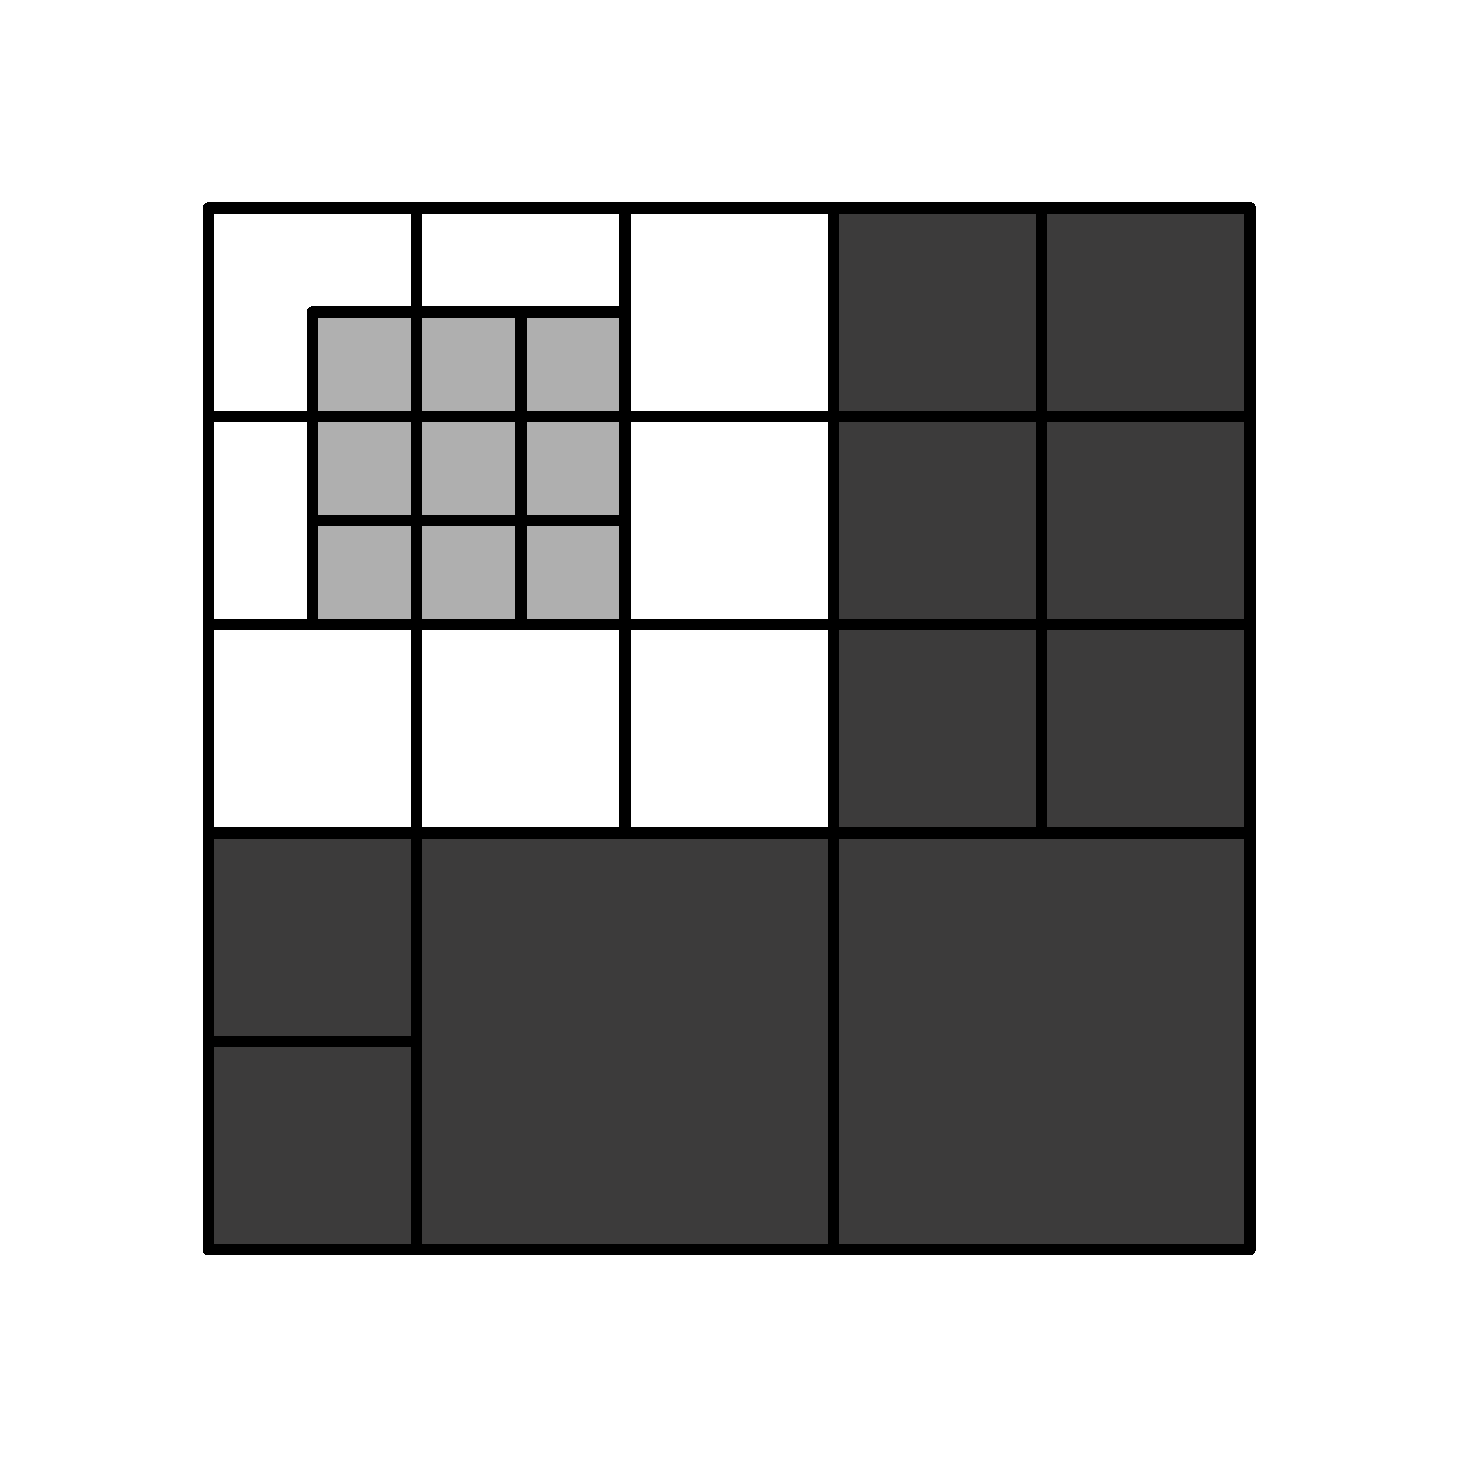
\includegraphics[width=.6\textwidth]{Images/N-body problems/FMMDecomp.pdf}};
    \begin{scope}[x={(image.south east)},y={(image.north west)}]
    \begin{scope}[x={(image.south east)},y={(image.north west)}]
        \node at (0.31,0.68) {$\underline{i}$};
    \end{scope}
    \end{scope}
\end{tikzpicture}
}
    \caption[Node $i$'s interactions for the original FMM algorithm.]{Node $i$'s interactions for the original FMM algorithm. The interaction with particles in the near neighbour nodes (light grey) will be computed on the subsequent division. The particles in the white boxes are in the interaction list of $i$ so will be computed through multipole expansions. Interaction of particles in the most distinct nodes (dark grey) has already been computed in previous divisions.}
    \label{fig:FMMDecomp}
\end{figure}

The tree is traversed downwards from level $2$ to the leaf nodes. Level $1$ and $2$ do not need to be considered as there are no node pairs that are well separated until at least three subdivisions are made. The multipole expansion (eq.~\ref{eq:FMMOuterSingle}) is used to compute the contribution to the potential of all particles in a node from other well-separated nodes. The interactions of particles in a node's current near neighbours need to be considered which cannot be done by a multipole expansion due to their proximity. However, considering the node on the level below containing the considered particle, by the above definitions, this node will have a new set of near and well-separated nodes. These well-separated nodes contain, by definition, particles which were in the near neighbour nodes and can now be considered by multipole expansions. This process is continued until the bottom of the tree is reached and where particle to particle interactions are considered as in the Barnes-Hut method. 

\begin{algorithm}
\caption{The exact $N \log N$ Algorithm}\label{alg:FMMNlogN}
\begin{algorithmic}
\State Decompose the domain into a tree structure until there is one particle per node
\For{For each particle $i$ traverse the tree in pre order (see \cref{appendix:Tree}) to compute total force on the particle}
    \State Decompose the domain into 16/64 nodes
    \State Compute the contribution of particles in nodes well separated from the node
    \State \; containing $i$ using multipole expansions.
    \Repeat
        \State Subdivide all nodes into 4/8 children nodes.
        \State For nodes in the interaction list of the node containing $i$ compute the 
        \State \; contribution of using multipole expansions
    \Until{One particle per node}
    \State Compute remaining interactions of near neighbour nodes directly
\EndFor
\end{algorithmic}
\end{algorithm}

This version of the Fast Multipole method computes in the same $\mathcal{O}(N\log N)$ as the Barnes-Hut method, however, it is capable of exact results due to the use of the multipole expansions. Numerically this is not possible as infinite terms are needed for each expansion, so the expansions are truncated to $p$ terms where each expansion has an error estimate of
\begin{equation*}
    \left|\phi(z)-Q \log (z)-\sum_{k=1}^{p} \frac{a_{k}}{z^{k}}\right| \leq A\left(\frac{1}{2}\right)^{p} \text{ where } A = \sum_{i=1}^{n} |q_i|
\end{equation*}
where $n$ is the number of particles involved in the expansion \cite{Beatson,Greengard1987ASimulations}. This means that at each level, $\mathcal{O}(N)$ amount of work needs to be done, each multipole expansion requires $\mathcal{O}(p)$ operations giving each level a complexity of $\mathcal{O}(Np)$. Assuming homogeneity, where the particles are evenly distributed, then there will be approximately $\mathcal{O}(\log N)$ levels giving the overall complexity as $\mathcal{O}(N\log N)$ with the total cost being $27Np\log N + 8N$ where the $8N$ is the number of direct interactions and the factor of $27$ comes from the maximum size of the interaction list. 

\subsubsection{\texorpdfstring{The $\mathcal{O}(N)$ Algorithm}{The O(N) Algorithm}} \label{subsec:OrderNFMM}
In order to reduce the algorithm from $\mathcal{O}(N\log N)$ to $\mathcal{O}(N)$ better use of the multipole expansions need to be made. Greengard and Rokhlin proposed to further expand the multipole expansions, this time locally around the centre of a node $z_0$ such that all particles in a node can be considered using a single expansion.
By translating equation \cref{eq:FMMOuterSingle} to the centre of the node and again summing over all charges, the expansion takes the form
\begin{equation}
\label{eq:FMMOuterMultiTrans1}
    \phi(z) = a_0\log(z-z_0) + \sum_{k=1}^\infty \frac{b_k}{(z-z_0)^k}
\end{equation}
A further Taylor expansion with respect to $z_0$ now obtains the multipole expansion of a set of potentials located in a circle of radius $R$ centred at $z_0$ for a point outside a circle of radius $R+|z_0|$ at the origin as
\begin{equation}
\label{eq:FMMOuterMultiTrans2}
\begin{gathered}
    \phi(z) = a_0\log(z) + \sum_{k=1}^\infty \frac{b_k}{z^k} \quad \text{ where } \\
    a_0 = \sum_{i=1}^n q_i \quad \text{ and } \quad b_k = -\frac{a_0 z_0^k}{k} + \sum_{l=1}^{k} a_l z_0^{k-l} \binom{k-1}{l-1}
\end{gathered}
\end{equation}
with $\binom{k}{l}$ being the binomial coefficients.

While \cref{eq:FMMOuterMulti,eq:FMMOuterMultiTrans1} allow for the calculation of the potential away from a cluster of particles, the potential inside a circle $D_1$ also needs to be calculated. Considering a group of charges inside a circle $D_2$ with radius $R$ centred at $z_0$, with $|z_0|>(c+1)R$ with $c>1$. The potential at the origin can be found using \cref{eq:FMMOuterMultiTrans1} and then the potential can be expanded locally about the origin to be able to calculate the potential at a point inside the circle $D_1$ of radius $R$ centred at the origin as
\begin{equation}
\label{eq:FMMInner}
\begin{gathered}
    \phi(z) = \sum_{k=0}^\infty \frac{b_k}{z^k} \quad \text{ where } \\
    b_0 = a_0\log(-z_0) + \sum_{l=1}^\infty \frac{a_l}{z_0^l}(-1)^l \text{ and } \\
    b_k = -\frac{a_0}{k\cdot z_0^k} + \sum_{l=1}^{k} \frac{a_l}{z_0^{l}} \binom{l+k-1}{l-1}(-1)^l, \text{ for } l>0.
\end{gathered}
\end{equation}
This is obtained through a Maclaurin expansion about the point $z$, the full derivation can be seen in Beatson and Greengard \cite{Beatson}. The centre of this expansion can be translated using the following relation
\begin{equation}
    \label{eq:LocalTranslation}
    \sum_{k=0}^p a_k(z-z_0)^p = \sum_{k=0}^{p} \left( \sum_{l=k}^p a_k \binom{l}{k})(-z_0)^{l-1} \right)z^k.
\end{equation}

\begin{figure}
    \centering
        \resizebox{.5\linewidth}{!}{\begin{tikzpicture}
    \node[anchor = south west,inner sep=0] (image) at (0,0) {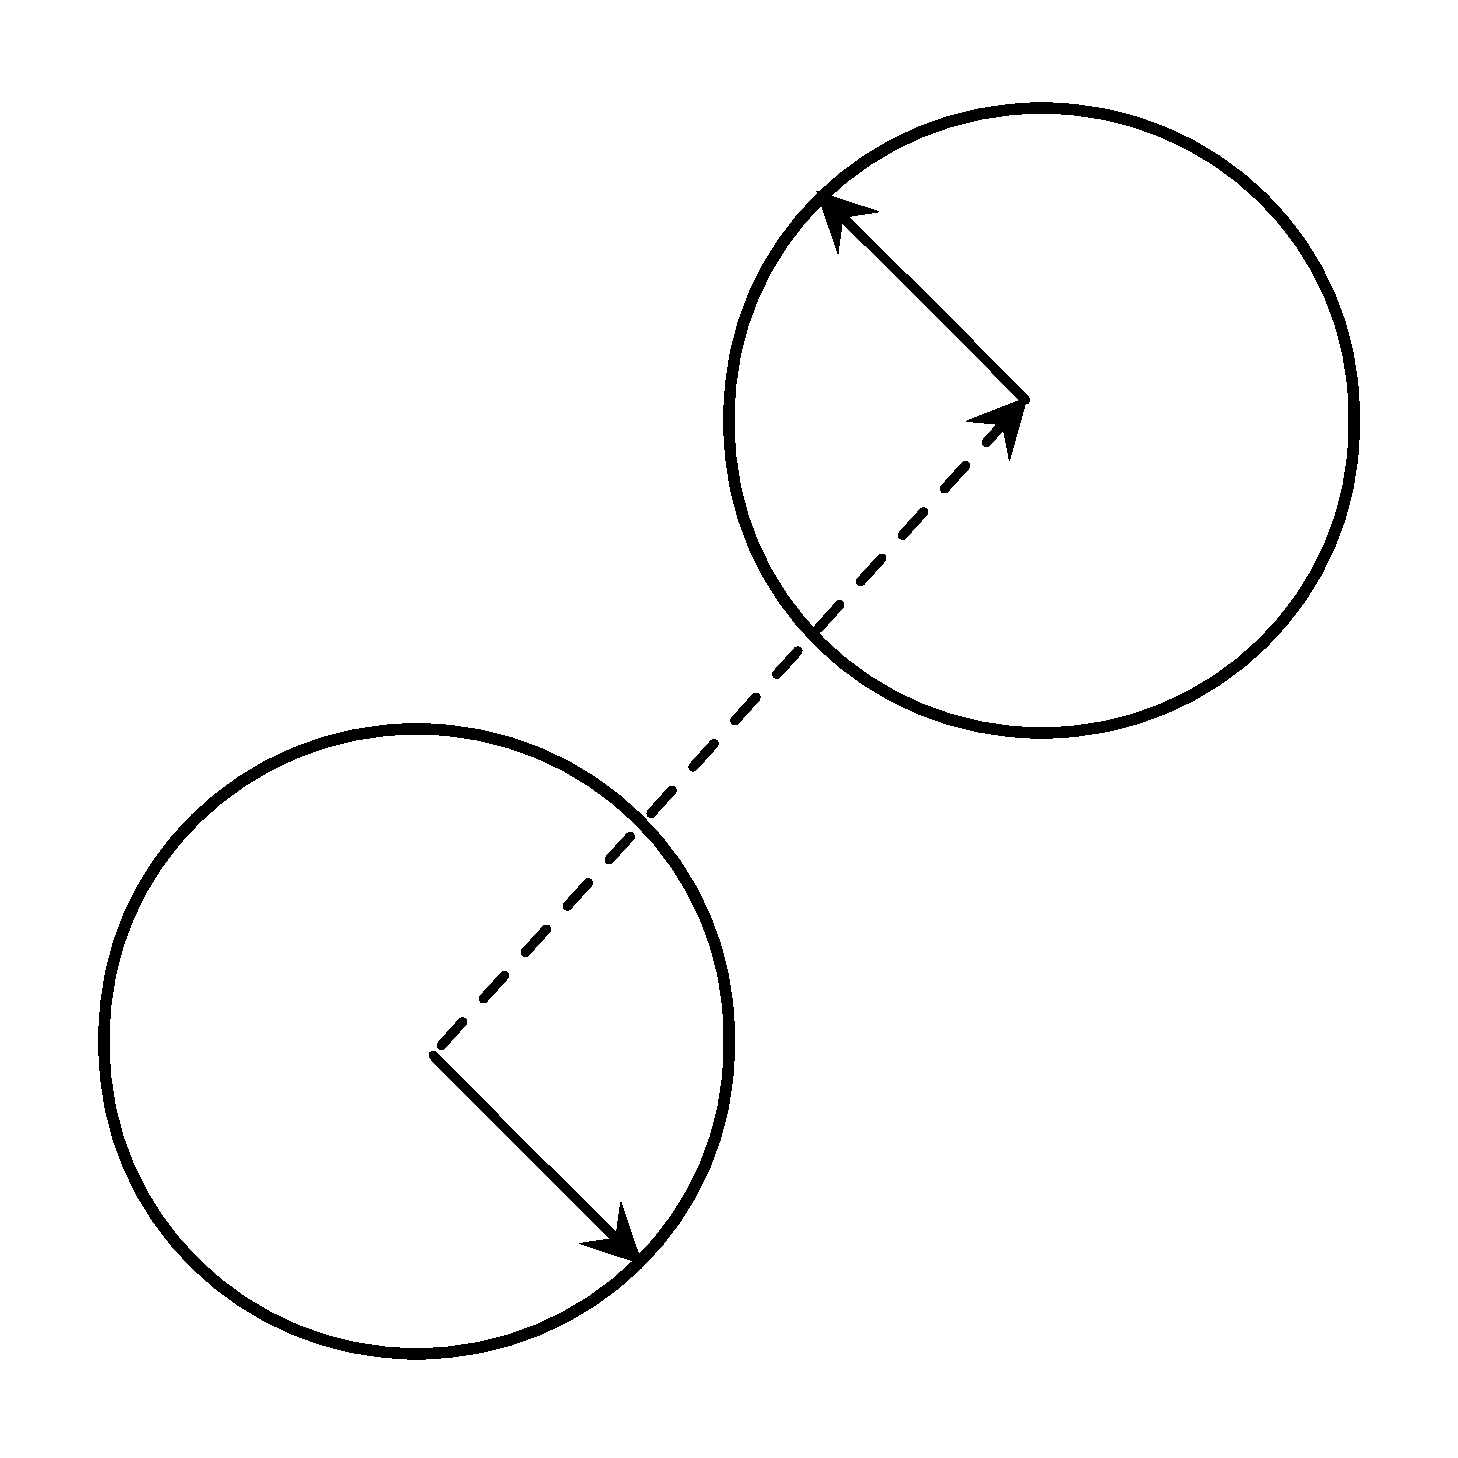
\includegraphics[width=.6\textwidth]{Images/KIFMM/Translation.pdf}};
    \begin{scope}[x={(image.south east)},y={(image.north west)}]
    \begin{scope}[x={(image.south east)},y={(image.north west)}]
        \node at (0.32,0.2) {$R$};
        \node at (0.70,0.8) {$R$};
        
        \node at (0.27,0.26) {$0$};
        \node at (0.74,0.73) {$z_0$};
        
        \node at (0.57,0.46) {$(c+1)R$};
        
        \node at (0.78,0.6) {$D_2$};
        \node at (0.2,0.4) {$D_1$};
    \end{scope}
    \end{scope}
\end{tikzpicture}
}
    \caption{Source charges $q_1,\dots,q_n$ are contained in the circle $D_2$. The corresponding expansion about $z_0$ converges inside $D_1$.}
    \label{fig:Translation}
\end{figure}

These expansions have the benefit of allowing for the evaluation of multipole expansions without the need to sum over all particles within that node. In particular, \cref{eq:FMMOuterMultiTrans2} allows for the calculation of the multipole expansion for all particles within a node by translating and summing over the expansions of the children nodes. In the downward pass, the method uses \cref{eq:LocalTranslation} to transmit the information of potentials outside of its near neighbours to its children.

The order $\mathcal{O}(N)$ is based on the $\mathcal{O}(N\log N)$ algorithm described in \cref{alg:FMMNlogN}, for simplicity we will only note the differences in the two methods here. Instead of decomposing the domain during the downward traversal of the tree, the tree is decomposed initially before any velocities are calculated. As the multipole expansions can be evaluated for any number of charges we only subdivide until there are at most $s$ particles per node at the finest level. As with the Barnes-Hut algorithm, the algorithm works from the bottom of the tree in post order. For leaf nodes, a truncated multipole expansion of $p$ terms is calculated based on the particles in the node. The expansions for all boxes in higher levels are then formed by shifting the expansions of all children nodes to the centre of the node and summing over coefficient terms.

Now that the upwards pass has formed a multipole expansion for each node based on all particles contained in it, the algorithm traverses down the tree computing node to node interactions. Instead of using the multipole expansions to calculate the effect of a node on a single particle, the method uses \cref{eq:FMMInner} to expand the multipole expansion of nodes in the interaction list into a local expansion which is valid inside the whole node. This expansion can then be shifted to the children of the node using \cref{eq:LocalTranslation} where the nodes in the childrens' interaction list is considered in the subsequent iteration.  After traversing the whole tree, each node on the highest level of a tree has a multipole expansion which takes into account all particles which are not in near neighbour nodes. The expansions can  be evaluated at all particle positions and then particle to particle interactions can be considered for all remaining particles. This three-step process is illustrated in \cref{fig:3Step} where the interactions between two well-separated nodes $A$ and $B$ are computed though the direct produce and through the use of multipole expansions.

\begin{figure}
    \centering
        \resizebox{.6\linewidth}{!}{\begin{tikzpicture}
    \node[anchor = south west,inner sep=0] (image) at (0,0) {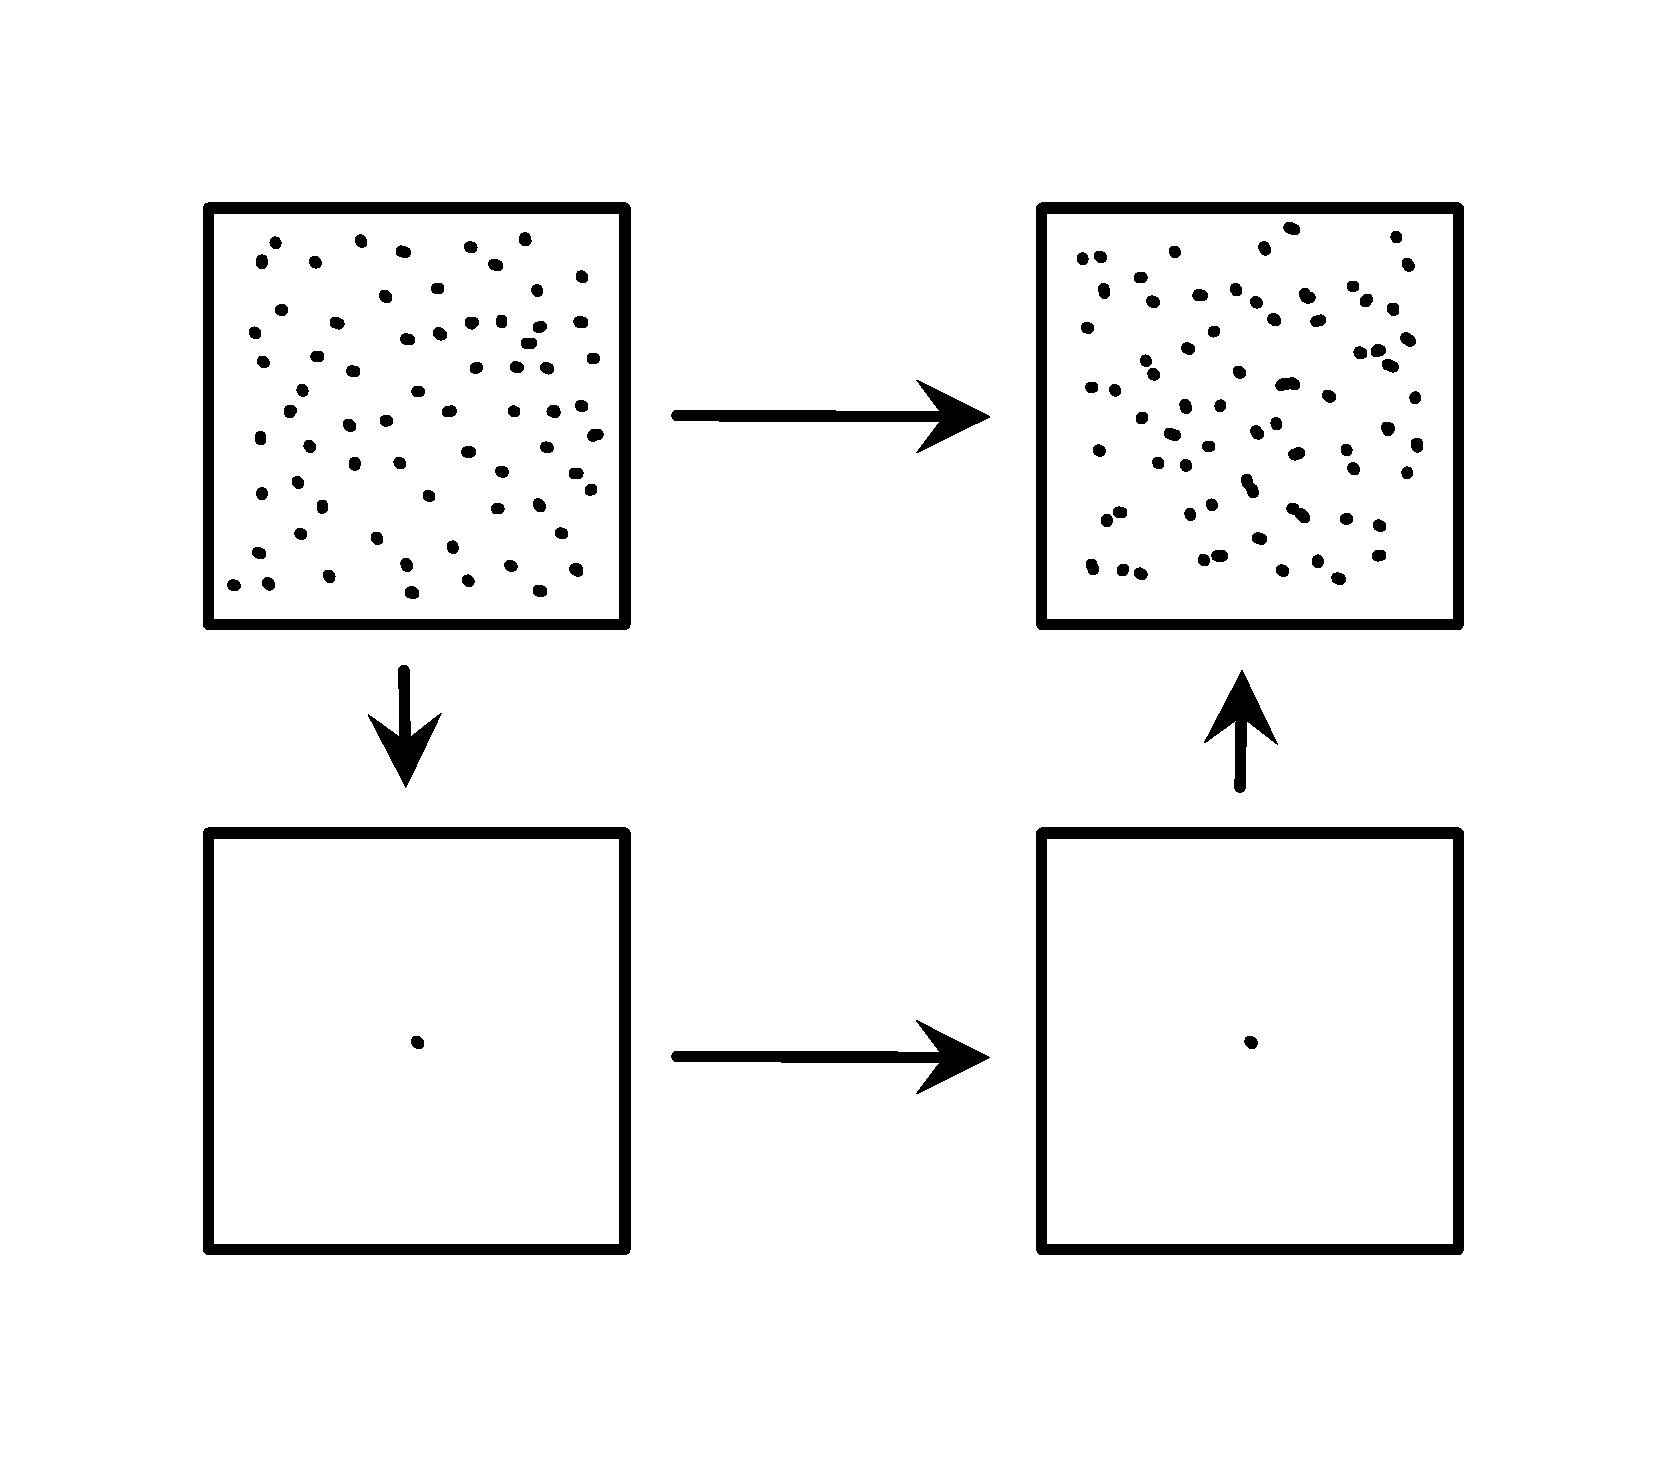
\includegraphics[width=.6\textwidth]{Images/KIFMM/3 Step.pdf}};
    \begin{scope}[x={(image.south east)},y={(image.north west)}]
    \begin{scope}[x={(image.south east)},y={(image.north west)}]
        \node at (0.25,0.9) {$A$};
        \node at (0.75,0.9) {$B$};
        
        \node at (0.25,0.22) {$C_A$};
        \node at (0.75,0.22) {$C_B$};
    
        \node at (0.5,0.78) {$\mathcal{O}(N^2)$};
        \node at (0.5,0.34) {$\mathcal{O}(1)$};
        \node at (0.35,0.5) {$\mathcal{O}(N)$};
        \node at (0.65,0.5) {$\mathcal{O}(N)$};
    \end{scope}
    \end{scope}
\end{tikzpicture}
}
    \caption[A diagram illustrating the three-step process FMM uses to reduce the complexity of $N$-body interactions from $\mathcal{O}(N^2)$ to $\mathcal{O}(N)$.]{A diagram illustrating the three-step process FMM uses to reduce the complexity of $N$-body interactions from $\mathcal{O}(N^2)$ to $\mathcal{O}(N)$. Assuming nodes $A$ and $B$ both have $N$ particles then directly computing the interaction takes $\mathcal{O}(N^2)$ operations. Taking the three-step process of computing the multipole expansion, translating the expansion and evaluation at the target points requires $\mathcal{O}(N)$ operations.
    }
    \label{fig:3Step}
\end{figure}

This three-step approach for calculating the interaction between two boxes yields an algorithm with total complexity $\mathcal{O}(N)$. In two dimensions the upwards pass takes $\mathcal{O}(Np)$ operations to calculate the multipole expansions for each node, $\mathcal{O}(29 \left(\frac{N}{s}\right) p^2)$ to shift the expansions between nodes, $\mathcal{O}(Np)$ operations to evaluate the local expansions and finally $\mathcal{O}(9Ns)$ operations to compute the near neighbour interactions. In three dimensions the total number of operations is of the order of $189\left(\frac{N}{s}\right)p^4 + 2Np^2 + 27Ns$. This means that the cost of increasing the accuracy of the original FMM algorithm in three dimensions grows to $\mathcal{O}(p^4)$, however, more recent work on the highly analytical structure of the FMM algorithm has allowed for the reduction of the cost of higher-order multipole expansions. Through the rotation of the nodes the work needed to translate the expansions has been decreased to $\mathcal{O}(p^4)$ to $\mathcal{O}(p^3)$ \cite{Greengard1997ADimensions,Hrycak1998AnFields} and even to $\mathcal{O}(p^2)$ by diagonalising the translations \cite{Berman2006Grid-MultipoleCalculations,Elliott1996FastAlgorithm}, however, these introduce numerical instabilities into the algorithm. The latest generation of FMMs are based on combining multipole expansions with plane wave expansions \cite{Greengard1997ADimensions,Hrycak1998AnFields} allowing for numerically stable calculations in three dimensions with a dependence on $p$ of only $\mathcal{O}(p^2)$ calculations. 

The multipole expansions presented here are derived from the two dimensional Coulomb potential and are taken from \cite{Beatson,Greengard1987ASimulations}. Adaptation to three dimensional systems proves more analytically complicated but follows the same structure as the two dimensional case. Derivation of the multipole expansions in three dimensions typically involves the use of spherical harmonics, and the translations are more computationally complicated to evaluate. The adaptions to the algorithm can be seen in detail along with the full derivation of the expansions, translations and error estimates, in Greengard and Rokhlin (1987) \cite{Greengard1987ASimulations} and Beatson and Greengard (1997) \cite{Beatson}. The FMM is widely used and has been deployed in stellar dynamics as an improvement to the Barnes-Hut algorithm \cite{Dehnen2014ADynamics}, in heat conduction \cite{Watschinger2021AEquation} and in non regularised Stokes flow \cite{Selmi2007FastComplexity,Tornberg2008}. The only problem with the standard FMM algorithms is the need to calculate multipole expansions for each kernel independently which can be difficult in cases such as the case of the stokeslet kernel. We will now look at an adaption to the FMM algorithm to create a Kernel Independent Fast Multipole (KIFMM) algorithm proposed by Ying \cite{Ying2004,Ying2005}.
\section{Kernel-Independent Fast Multipole Method}
If we consider a many body problem formed of $N$ potential/quadrature points $\{{\bm{y}}_n\}$ each with an associated potential/force $\{{\bm{f}}_n\}$ that we will evaluate on $M$ collocation points $\{\bm{x}_m\}$ then we can compute the velocity at each $\bm{x}_m$ where $m=1,2,\dots,M$ through
\begin{equation*}
    \bm{u}(\bm{x}) = \sum_{i=1}^N \Phi(\bm{x},{\bm{y}}_i){\bm{f}}_i
\end{equation*}
where $\Phi$ is the green's function associated with the underlying partial differential equation governing the dynamics of the system. In particular, $\Phi=S^\epsilon$ is our kernel for the case of the method of regularised Stokeslets where we compute the velocity of the fluid at a set of collocation points based on a set of body forces defined on solid boundaries within the fluid. This can be written as a matrix-vector product as described in \cref{eq:matrixvectorproduct}. This direct solution has a computational complexity of $\mathcal{O}(NM)$ which for either a large number of collocation points or quadrature points quickly becomes prohibitive due. In order to compute large systems we need to look at faster methods to approximate this vector-matrix product. One such set of methods is the familiy of fast multipole method's which can approximate \cref{eq:matrixvectorproduct} with complexity $\mathcal{O}(N+M)$. The standard fast multipole method (FMM) algorithm uses multipole expansion's of the kernel about the quadrature points in order to approximate long-range interaction between distant quadrature and target points \cite{Beatson,Tornberg2008,Wang2007AEquations,Yokota}. This method proves time-consuming to find for particular kernels such as regularised Stokeslets where the corresponding expansions first need to be computed by hand, it also means that the entire program is kernel dependent and any changes to the kernel need a complete recalculation of the expansions employed.
Instead we will look at an adaption to the FMM algorithm to create a kernel independent fast multipole algorithm (KIFMM) \cite{Ying2004, Ying2005,Rostami2016Kernel-independentStokeslets,Yan}. Using equivalent potentials instead of multipole expansions we can approximate long-range interactions using only kernel evaluations without computing every particle to particle interaction. This dramatically reduces the number of kernel evaluations compared to computation by the direct solution. 

\subsection{Hierarchical decomposition of the computational domain}
Both FMM and KIFMM are based on the Hierarchical decomposition of the computational domain. We let $\mathcal{D}$ be the computational domain, which we define to be a cube in $\mathcal{R}^3$ such that it encompasses all points in $\{\bm{y}_n\}$ and $\{\bm{x}_m\}$. We typically define this to be the smallest possible cube which includes all the points. The FMM method builds an Octree structure of cubes in 3D with the cube $\mathcal{D}$ as the root node. We will label this node the Level $0$ partition where no subdivision had occurred. Each subsequent division is made of $8$ equal-sized cubes each with a side length of half of the cube above. For each level, we subdivide a node into its $8$ children if the number of source points or target points within the cube is greater than some threshold $s\geq 1$. For efficiency only points of the type which exceed the threshold are moved from to the child nodes. This subdivision creates a new level $L+1$ containing the children of all subdivided nodes in level $L$. We refer to the node on level $L$ as the parent of nodes on level $L+1$. This process is repeated until all cubes have less than $s$ source or target points contained within them which we will refer to as leaf nodes.

\begin{figure}[ht]
    \centering
    \resizebox{.6\linewidth}{!}{% This file was created by matlab2tikz.
%
%The latest updates can be retrieved from
%  http://www.mathworks.com/matlabcentral/fileexchange/22022-matlab2tikz-matlab2tikz
%where you can also make suggestions and rate matlab2tikz.
%
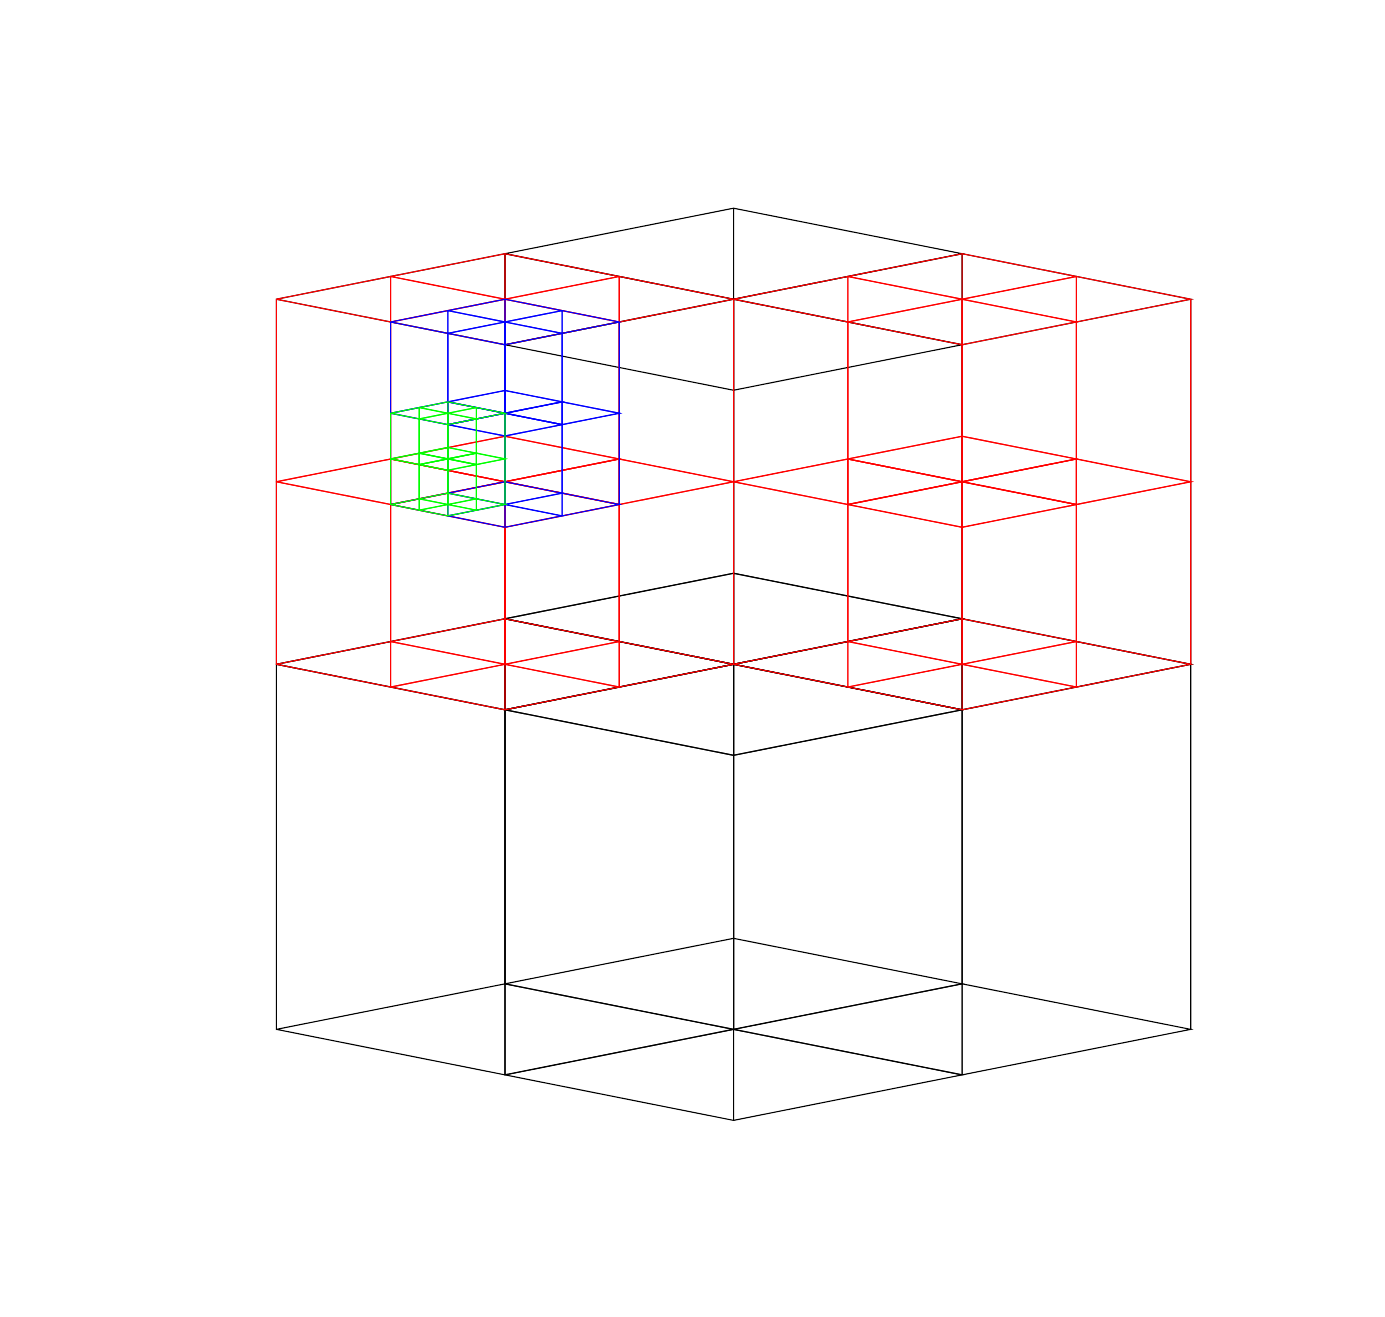
\begin{tikzpicture}

\begin{axis}[%
width=5.151in,
height=5.139in,
at={(0.864in,0.694in)},
scale only axis,
unbounded coords=jump,
xmin=0,
xmax=1,
tick align=outside,
ymin=0,
ymax=1,
zmin=0,
zmax=1,
view={45}{10},
axis line style={draw=none},
ticks=none,
axis x line*=bottom,
axis y line*=left,
axis z line*=left
]
\addplot3 [color=black]
 table[row sep=crcr] {%
0.0737015537421595	0.0737015537421595	0.0737015537421595\\
0.517448266926349	0.0737015537421595	0.0737015537421595\\
0.517448266926349	0.517448266926349	0.0737015537421595\\
0.0737015537421595	0.517448266926349	0.0737015537421595\\
0.0737015537421595	0.0737015537421595	0.0737015537421595\\
0.0737015537421595	0.0737015537421595	0.517448266926349\\
0.517448266926349	0.0737015537421595	0.517448266926349\\
0.517448266926349	0.517448266926349	0.517448266926349\\
0.0737015537421595	0.517448266926349	0.517448266926349\\
0.0737015537421595	0.0737015537421595	0.517448266926349\\
0.0737015537421595	0.0737015537421595	0.0737015537421595\\
nan	nan	nan\\
0.517448266926349	0.0737015537421595	0.0737015537421595\\
0.517448266926349	0.0737015537421595	0.517448266926349\\
nan	nan	nan\\
0.517448266926349	0.517448266926349	0.0737015537421595\\
0.517448266926349	0.517448266926349	0.517448266926349\\
nan	nan	nan\\
0.0737015537421595	0.517448266926349	0.0737015537421595\\
0.0737015537421595	0.517448266926349	0.517448266926349\\
};
 \addplot3 [color=black]
 table[row sep=crcr] {%
0.0737015537421595	0.0737015537421595	0.517448266926349\\
0.517448266926349	0.0737015537421595	0.517448266926349\\
0.517448266926349	0.517448266926349	0.517448266926349\\
0.0737015537421595	0.517448266926349	0.517448266926349\\
0.0737015537421595	0.0737015537421595	0.517448266926349\\
0.0737015537421595	0.0737015537421595	0.961194980110539\\
0.517448266926349	0.0737015537421595	0.961194980110539\\
0.517448266926349	0.517448266926349	0.961194980110539\\
0.0737015537421595	0.517448266926349	0.961194980110539\\
0.0737015537421595	0.0737015537421595	0.961194980110539\\
0.0737015537421595	0.0737015537421595	0.517448266926349\\
nan	nan	nan\\
0.517448266926349	0.0737015537421595	0.517448266926349\\
0.517448266926349	0.0737015537421595	0.961194980110539\\
nan	nan	nan\\
0.517448266926349	0.517448266926349	0.517448266926349\\
0.517448266926349	0.517448266926349	0.961194980110539\\
nan	nan	nan\\
0.0737015537421595	0.517448266926349	0.517448266926349\\
0.0737015537421595	0.517448266926349	0.961194980110539\\
};
 \addplot3 [color=black]
 table[row sep=crcr] {%
0.0737015537421595	0.517448266926349	0.0737015537421595\\
0.517448266926349	0.517448266926349	0.0737015537421595\\
0.517448266926349	0.961194980110539	0.0737015537421595\\
0.0737015537421595	0.961194980110539	0.0737015537421595\\
0.0737015537421595	0.517448266926349	0.0737015537421595\\
0.0737015537421595	0.517448266926349	0.517448266926349\\
0.517448266926349	0.517448266926349	0.517448266926349\\
0.517448266926349	0.961194980110539	0.517448266926349\\
0.0737015537421595	0.961194980110539	0.517448266926349\\
0.0737015537421595	0.517448266926349	0.517448266926349\\
0.0737015537421595	0.517448266926349	0.0737015537421595\\
nan	nan	nan\\
0.517448266926349	0.517448266926349	0.0737015537421595\\
0.517448266926349	0.517448266926349	0.517448266926349\\
nan	nan	nan\\
0.517448266926349	0.961194980110539	0.0737015537421595\\
0.517448266926349	0.961194980110539	0.517448266926349\\
nan	nan	nan\\
0.0737015537421595	0.961194980110539	0.0737015537421595\\
0.0737015537421595	0.961194980110539	0.517448266926349\\
};
 \addplot3 [color=black]
 table[row sep=crcr] {%
0.0737015537421595	0.517448266926349	0.517448266926349\\
0.517448266926349	0.517448266926349	0.517448266926349\\
0.517448266926349	0.961194980110539	0.517448266926349\\
0.0737015537421595	0.961194980110539	0.517448266926349\\
0.0737015537421595	0.517448266926349	0.517448266926349\\
0.0737015537421595	0.517448266926349	0.961194980110539\\
0.517448266926349	0.517448266926349	0.961194980110539\\
0.517448266926349	0.961194980110539	0.961194980110539\\
0.0737015537421595	0.961194980110539	0.961194980110539\\
0.0737015537421595	0.517448266926349	0.961194980110539\\
0.0737015537421595	0.517448266926349	0.517448266926349\\
nan	nan	nan\\
0.517448266926349	0.517448266926349	0.517448266926349\\
0.517448266926349	0.517448266926349	0.961194980110539\\
nan	nan	nan\\
0.517448266926349	0.961194980110539	0.517448266926349\\
0.517448266926349	0.961194980110539	0.961194980110539\\
nan	nan	nan\\
0.0737015537421595	0.961194980110539	0.517448266926349\\
0.0737015537421595	0.961194980110539	0.961194980110539\\
};
 \addplot3 [color=black]
 table[row sep=crcr] {%
0.517448266926349	0.0737015537421595	0.0737015537421595\\
0.961194980110539	0.0737015537421595	0.0737015537421595\\
0.961194980110539	0.517448266926349	0.0737015537421595\\
0.517448266926349	0.517448266926349	0.0737015537421595\\
0.517448266926349	0.0737015537421595	0.0737015537421595\\
0.517448266926349	0.0737015537421595	0.517448266926349\\
0.961194980110539	0.0737015537421595	0.517448266926349\\
0.961194980110539	0.517448266926349	0.517448266926349\\
0.517448266926349	0.517448266926349	0.517448266926349\\
0.517448266926349	0.0737015537421595	0.517448266926349\\
0.517448266926349	0.0737015537421595	0.0737015537421595\\
nan	nan	nan\\
0.961194980110539	0.0737015537421595	0.0737015537421595\\
0.961194980110539	0.0737015537421595	0.517448266926349\\
nan	nan	nan\\
0.961194980110539	0.517448266926349	0.0737015537421595\\
0.961194980110539	0.517448266926349	0.517448266926349\\
nan	nan	nan\\
0.517448266926349	0.517448266926349	0.0737015537421595\\
0.517448266926349	0.517448266926349	0.517448266926349\\
};
 \addplot3 [color=black]
 table[row sep=crcr] {%
0.517448266926349	0.0737015537421595	0.517448266926349\\
0.961194980110539	0.0737015537421595	0.517448266926349\\
0.961194980110539	0.517448266926349	0.517448266926349\\
0.517448266926349	0.517448266926349	0.517448266926349\\
0.517448266926349	0.0737015537421595	0.517448266926349\\
0.517448266926349	0.0737015537421595	0.961194980110539\\
0.961194980110539	0.0737015537421595	0.961194980110539\\
0.961194980110539	0.517448266926349	0.961194980110539\\
0.517448266926349	0.517448266926349	0.961194980110539\\
0.517448266926349	0.0737015537421595	0.961194980110539\\
0.517448266926349	0.0737015537421595	0.517448266926349\\
nan	nan	nan\\
0.961194980110539	0.0737015537421595	0.517448266926349\\
0.961194980110539	0.0737015537421595	0.961194980110539\\
nan	nan	nan\\
0.961194980110539	0.517448266926349	0.517448266926349\\
0.961194980110539	0.517448266926349	0.961194980110539\\
nan	nan	nan\\
0.517448266926349	0.517448266926349	0.517448266926349\\
0.517448266926349	0.517448266926349	0.961194980110539\\
};
 \addplot3 [color=black]
 table[row sep=crcr] {%
0.517448266926349	0.517448266926349	0.0737015537421595\\
0.961194980110539	0.517448266926349	0.0737015537421595\\
0.961194980110539	0.961194980110539	0.0737015537421595\\
0.517448266926349	0.961194980110539	0.0737015537421595\\
0.517448266926349	0.517448266926349	0.0737015537421595\\
0.517448266926349	0.517448266926349	0.517448266926349\\
0.961194980110539	0.517448266926349	0.517448266926349\\
0.961194980110539	0.961194980110539	0.517448266926349\\
0.517448266926349	0.961194980110539	0.517448266926349\\
0.517448266926349	0.517448266926349	0.517448266926349\\
0.517448266926349	0.517448266926349	0.0737015537421595\\
nan	nan	nan\\
0.961194980110539	0.517448266926349	0.0737015537421595\\
0.961194980110539	0.517448266926349	0.517448266926349\\
nan	nan	nan\\
0.961194980110539	0.961194980110539	0.0737015537421595\\
0.961194980110539	0.961194980110539	0.517448266926349\\
nan	nan	nan\\
0.517448266926349	0.961194980110539	0.0737015537421595\\
0.517448266926349	0.961194980110539	0.517448266926349\\
};
 \addplot3 [color=black]
 table[row sep=crcr] {%
0.517448266926349	0.517448266926349	0.517448266926349\\
0.961194980110539	0.517448266926349	0.517448266926349\\
0.961194980110539	0.961194980110539	0.517448266926349\\
0.517448266926349	0.961194980110539	0.517448266926349\\
0.517448266926349	0.517448266926349	0.517448266926349\\
0.517448266926349	0.517448266926349	0.961194980110539\\
0.961194980110539	0.517448266926349	0.961194980110539\\
0.961194980110539	0.961194980110539	0.961194980110539\\
0.517448266926349	0.961194980110539	0.961194980110539\\
0.517448266926349	0.517448266926349	0.961194980110539\\
0.517448266926349	0.517448266926349	0.517448266926349\\
nan	nan	nan\\
0.961194980110539	0.517448266926349	0.517448266926349\\
0.961194980110539	0.517448266926349	0.961194980110539\\
nan	nan	nan\\
0.961194980110539	0.961194980110539	0.517448266926349\\
0.961194980110539	0.961194980110539	0.961194980110539\\
nan	nan	nan\\
0.517448266926349	0.961194980110539	0.517448266926349\\
0.517448266926349	0.961194980110539	0.961194980110539\\
};
 \addplot3 [color=red]
 table[row sep=crcr] {%
0.0737015537421595	0.0737015537421595	0.517448266926349\\
0.295574910334254	0.0737015537421595	0.517448266926349\\
0.295574910334254	0.295574910334254	0.517448266926349\\
0.0737015537421595	0.295574910334254	0.517448266926349\\
0.0737015537421595	0.0737015537421595	0.517448266926349\\
0.0737015537421595	0.0737015537421595	0.739321623518444\\
0.295574910334254	0.0737015537421595	0.739321623518444\\
0.295574910334254	0.295574910334254	0.739321623518444\\
0.0737015537421595	0.295574910334254	0.739321623518444\\
0.0737015537421595	0.0737015537421595	0.739321623518444\\
0.0737015537421595	0.0737015537421595	0.517448266926349\\
nan	nan	nan\\
0.295574910334254	0.0737015537421595	0.517448266926349\\
0.295574910334254	0.0737015537421595	0.739321623518444\\
nan	nan	nan\\
0.295574910334254	0.295574910334254	0.517448266926349\\
0.295574910334254	0.295574910334254	0.739321623518444\\
nan	nan	nan\\
0.0737015537421595	0.295574910334254	0.517448266926349\\
0.0737015537421595	0.295574910334254	0.739321623518444\\
};
 \addplot3 [color=red]
 table[row sep=crcr] {%
0.0737015537421595	0.0737015537421595	0.739321623518444\\
0.295574910334254	0.0737015537421595	0.739321623518444\\
0.295574910334254	0.295574910334254	0.739321623518444\\
0.0737015537421595	0.295574910334254	0.739321623518444\\
0.0737015537421595	0.0737015537421595	0.739321623518444\\
0.0737015537421595	0.0737015537421595	0.961194980110539\\
0.295574910334254	0.0737015537421595	0.961194980110539\\
0.295574910334254	0.295574910334254	0.961194980110539\\
0.0737015537421595	0.295574910334254	0.961194980110539\\
0.0737015537421595	0.0737015537421595	0.961194980110539\\
0.0737015537421595	0.0737015537421595	0.739321623518444\\
nan	nan	nan\\
0.295574910334254	0.0737015537421595	0.739321623518444\\
0.295574910334254	0.0737015537421595	0.961194980110539\\
nan	nan	nan\\
0.295574910334254	0.295574910334254	0.739321623518444\\
0.295574910334254	0.295574910334254	0.961194980110539\\
nan	nan	nan\\
0.0737015537421595	0.295574910334254	0.739321623518444\\
0.0737015537421595	0.295574910334254	0.961194980110539\\
};
 \addplot3 [color=red]
 table[row sep=crcr] {%
0.0737015537421595	0.295574910334254	0.517448266926349\\
0.295574910334254	0.295574910334254	0.517448266926349\\
0.295574910334254	0.517448266926349	0.517448266926349\\
0.0737015537421595	0.517448266926349	0.517448266926349\\
0.0737015537421595	0.295574910334254	0.517448266926349\\
0.0737015537421595	0.295574910334254	0.739321623518444\\
0.295574910334254	0.295574910334254	0.739321623518444\\
0.295574910334254	0.517448266926349	0.739321623518444\\
0.0737015537421595	0.517448266926349	0.739321623518444\\
0.0737015537421595	0.295574910334254	0.739321623518444\\
0.0737015537421595	0.295574910334254	0.517448266926349\\
nan	nan	nan\\
0.295574910334254	0.295574910334254	0.517448266926349\\
0.295574910334254	0.295574910334254	0.739321623518444\\
nan	nan	nan\\
0.295574910334254	0.517448266926349	0.517448266926349\\
0.295574910334254	0.517448266926349	0.739321623518444\\
nan	nan	nan\\
0.0737015537421595	0.517448266926349	0.517448266926349\\
0.0737015537421595	0.517448266926349	0.739321623518444\\
};
 \addplot3 [color=red]
 table[row sep=crcr] {%
0.0737015537421595	0.295574910334254	0.739321623518444\\
0.295574910334254	0.295574910334254	0.739321623518444\\
0.295574910334254	0.517448266926349	0.739321623518444\\
0.0737015537421595	0.517448266926349	0.739321623518444\\
0.0737015537421595	0.295574910334254	0.739321623518444\\
0.0737015537421595	0.295574910334254	0.961194980110539\\
0.295574910334254	0.295574910334254	0.961194980110539\\
0.295574910334254	0.517448266926349	0.961194980110539\\
0.0737015537421595	0.517448266926349	0.961194980110539\\
0.0737015537421595	0.295574910334254	0.961194980110539\\
0.0737015537421595	0.295574910334254	0.739321623518444\\
nan	nan	nan\\
0.295574910334254	0.295574910334254	0.739321623518444\\
0.295574910334254	0.295574910334254	0.961194980110539\\
nan	nan	nan\\
0.295574910334254	0.517448266926349	0.739321623518444\\
0.295574910334254	0.517448266926349	0.961194980110539\\
nan	nan	nan\\
0.0737015537421595	0.517448266926349	0.739321623518444\\
0.0737015537421595	0.517448266926349	0.961194980110539\\
};
 \addplot3 [color=red]
 table[row sep=crcr] {%
0.295574910334254	0.0737015537421595	0.517448266926349\\
0.517448266926349	0.0737015537421595	0.517448266926349\\
0.517448266926349	0.295574910334254	0.517448266926349\\
0.295574910334254	0.295574910334254	0.517448266926349\\
0.295574910334254	0.0737015537421595	0.517448266926349\\
0.295574910334254	0.0737015537421595	0.739321623518444\\
0.517448266926349	0.0737015537421595	0.739321623518444\\
0.517448266926349	0.295574910334254	0.739321623518444\\
0.295574910334254	0.295574910334254	0.739321623518444\\
0.295574910334254	0.0737015537421595	0.739321623518444\\
0.295574910334254	0.0737015537421595	0.517448266926349\\
nan	nan	nan\\
0.517448266926349	0.0737015537421595	0.517448266926349\\
0.517448266926349	0.0737015537421595	0.739321623518444\\
nan	nan	nan\\
0.517448266926349	0.295574910334254	0.517448266926349\\
0.517448266926349	0.295574910334254	0.739321623518444\\
nan	nan	nan\\
0.295574910334254	0.295574910334254	0.517448266926349\\
0.295574910334254	0.295574910334254	0.739321623518444\\
};
 \addplot3 [color=red]
 table[row sep=crcr] {%
0.295574910334254	0.0737015537421595	0.739321623518444\\
0.517448266926349	0.0737015537421595	0.739321623518444\\
0.517448266926349	0.295574910334254	0.739321623518444\\
0.295574910334254	0.295574910334254	0.739321623518444\\
0.295574910334254	0.0737015537421595	0.739321623518444\\
0.295574910334254	0.0737015537421595	0.961194980110539\\
0.517448266926349	0.0737015537421595	0.961194980110539\\
0.517448266926349	0.295574910334254	0.961194980110539\\
0.295574910334254	0.295574910334254	0.961194980110539\\
0.295574910334254	0.0737015537421595	0.961194980110539\\
0.295574910334254	0.0737015537421595	0.739321623518444\\
nan	nan	nan\\
0.517448266926349	0.0737015537421595	0.739321623518444\\
0.517448266926349	0.0737015537421595	0.961194980110539\\
nan	nan	nan\\
0.517448266926349	0.295574910334254	0.739321623518444\\
0.517448266926349	0.295574910334254	0.961194980110539\\
nan	nan	nan\\
0.295574910334254	0.295574910334254	0.739321623518444\\
0.295574910334254	0.295574910334254	0.961194980110539\\
};
 \addplot3 [color=red]
 table[row sep=crcr] {%
0.295574910334254	0.295574910334254	0.517448266926349\\
0.517448266926349	0.295574910334254	0.517448266926349\\
0.517448266926349	0.517448266926349	0.517448266926349\\
0.295574910334254	0.517448266926349	0.517448266926349\\
0.295574910334254	0.295574910334254	0.517448266926349\\
0.295574910334254	0.295574910334254	0.739321623518444\\
0.517448266926349	0.295574910334254	0.739321623518444\\
0.517448266926349	0.517448266926349	0.739321623518444\\
0.295574910334254	0.517448266926349	0.739321623518444\\
0.295574910334254	0.295574910334254	0.739321623518444\\
0.295574910334254	0.295574910334254	0.517448266926349\\
nan	nan	nan\\
0.517448266926349	0.295574910334254	0.517448266926349\\
0.517448266926349	0.295574910334254	0.739321623518444\\
nan	nan	nan\\
0.517448266926349	0.517448266926349	0.517448266926349\\
0.517448266926349	0.517448266926349	0.739321623518444\\
nan	nan	nan\\
0.295574910334254	0.517448266926349	0.517448266926349\\
0.295574910334254	0.517448266926349	0.739321623518444\\
};
 \addplot3 [color=red]
 table[row sep=crcr] {%
0.295574910334254	0.295574910334254	0.739321623518444\\
0.517448266926349	0.295574910334254	0.739321623518444\\
0.517448266926349	0.517448266926349	0.739321623518444\\
0.295574910334254	0.517448266926349	0.739321623518444\\
0.295574910334254	0.295574910334254	0.739321623518444\\
0.295574910334254	0.295574910334254	0.961194980110539\\
0.517448266926349	0.295574910334254	0.961194980110539\\
0.517448266926349	0.517448266926349	0.961194980110539\\
0.295574910334254	0.517448266926349	0.961194980110539\\
0.295574910334254	0.295574910334254	0.961194980110539\\
0.295574910334254	0.295574910334254	0.739321623518444\\
nan	nan	nan\\
0.517448266926349	0.295574910334254	0.739321623518444\\
0.517448266926349	0.295574910334254	0.961194980110539\\
nan	nan	nan\\
0.517448266926349	0.517448266926349	0.739321623518444\\
0.517448266926349	0.517448266926349	0.961194980110539\\
nan	nan	nan\\
0.295574910334254	0.517448266926349	0.739321623518444\\
0.295574910334254	0.517448266926349	0.961194980110539\\
};
 \addplot3 [color=red]
 table[row sep=crcr] {%
0.517448266926349	0.517448266926349	0.517448266926349\\
0.739321623518444	0.517448266926349	0.517448266926349\\
0.739321623518444	0.739321623518444	0.517448266926349\\
0.517448266926349	0.739321623518444	0.517448266926349\\
0.517448266926349	0.517448266926349	0.517448266926349\\
0.517448266926349	0.517448266926349	0.739321623518444\\
0.739321623518444	0.517448266926349	0.739321623518444\\
0.739321623518444	0.739321623518444	0.739321623518444\\
0.517448266926349	0.739321623518444	0.739321623518444\\
0.517448266926349	0.517448266926349	0.739321623518444\\
0.517448266926349	0.517448266926349	0.517448266926349\\
nan	nan	nan\\
0.739321623518444	0.517448266926349	0.517448266926349\\
0.739321623518444	0.517448266926349	0.739321623518444\\
nan	nan	nan\\
0.739321623518444	0.739321623518444	0.517448266926349\\
0.739321623518444	0.739321623518444	0.739321623518444\\
nan	nan	nan\\
0.517448266926349	0.739321623518444	0.517448266926349\\
0.517448266926349	0.739321623518444	0.739321623518444\\
};
 \addplot3 [color=red]
 table[row sep=crcr] {%
0.517448266926349	0.517448266926349	0.739321623518444\\
0.739321623518444	0.517448266926349	0.739321623518444\\
0.739321623518444	0.739321623518444	0.739321623518444\\
0.517448266926349	0.739321623518444	0.739321623518444\\
0.517448266926349	0.517448266926349	0.739321623518444\\
0.517448266926349	0.517448266926349	0.961194980110539\\
0.739321623518444	0.517448266926349	0.961194980110539\\
0.739321623518444	0.739321623518444	0.961194980110539\\
0.517448266926349	0.739321623518444	0.961194980110539\\
0.517448266926349	0.517448266926349	0.961194980110539\\
0.517448266926349	0.517448266926349	0.739321623518444\\
nan	nan	nan\\
0.739321623518444	0.517448266926349	0.739321623518444\\
0.739321623518444	0.517448266926349	0.961194980110539\\
nan	nan	nan\\
0.739321623518444	0.739321623518444	0.739321623518444\\
0.739321623518444	0.739321623518444	0.961194980110539\\
nan	nan	nan\\
0.517448266926349	0.739321623518444	0.739321623518444\\
0.517448266926349	0.739321623518444	0.961194980110539\\
};
 \addplot3 [color=red]
 table[row sep=crcr] {%
0.517448266926349	0.739321623518444	0.517448266926349\\
0.739321623518444	0.739321623518444	0.517448266926349\\
0.739321623518444	0.961194980110539	0.517448266926349\\
0.517448266926349	0.961194980110539	0.517448266926349\\
0.517448266926349	0.739321623518444	0.517448266926349\\
0.517448266926349	0.739321623518444	0.739321623518444\\
0.739321623518444	0.739321623518444	0.739321623518444\\
0.739321623518444	0.961194980110539	0.739321623518444\\
0.517448266926349	0.961194980110539	0.739321623518444\\
0.517448266926349	0.739321623518444	0.739321623518444\\
0.517448266926349	0.739321623518444	0.517448266926349\\
nan	nan	nan\\
0.739321623518444	0.739321623518444	0.517448266926349\\
0.739321623518444	0.739321623518444	0.739321623518444\\
nan	nan	nan\\
0.739321623518444	0.961194980110539	0.517448266926349\\
0.739321623518444	0.961194980110539	0.739321623518444\\
nan	nan	nan\\
0.517448266926349	0.961194980110539	0.517448266926349\\
0.517448266926349	0.961194980110539	0.739321623518444\\
};
 \addplot3 [color=red]
 table[row sep=crcr] {%
0.517448266926349	0.739321623518444	0.739321623518444\\
0.739321623518444	0.739321623518444	0.739321623518444\\
0.739321623518444	0.961194980110539	0.739321623518444\\
0.517448266926349	0.961194980110539	0.739321623518444\\
0.517448266926349	0.739321623518444	0.739321623518444\\
0.517448266926349	0.739321623518444	0.961194980110539\\
0.739321623518444	0.739321623518444	0.961194980110539\\
0.739321623518444	0.961194980110539	0.961194980110539\\
0.517448266926349	0.961194980110539	0.961194980110539\\
0.517448266926349	0.739321623518444	0.961194980110539\\
0.517448266926349	0.739321623518444	0.739321623518444\\
nan	nan	nan\\
0.739321623518444	0.739321623518444	0.739321623518444\\
0.739321623518444	0.739321623518444	0.961194980110539\\
nan	nan	nan\\
0.739321623518444	0.961194980110539	0.739321623518444\\
0.739321623518444	0.961194980110539	0.961194980110539\\
nan	nan	nan\\
0.517448266926349	0.961194980110539	0.739321623518444\\
0.517448266926349	0.961194980110539	0.961194980110539\\
};
 \addplot3 [color=red]
 table[row sep=crcr] {%
0.739321623518444	0.517448266926349	0.517448266926349\\
0.961194980110539	0.517448266926349	0.517448266926349\\
0.961194980110539	0.739321623518444	0.517448266926349\\
0.739321623518444	0.739321623518444	0.517448266926349\\
0.739321623518444	0.517448266926349	0.517448266926349\\
0.739321623518444	0.517448266926349	0.739321623518444\\
0.961194980110539	0.517448266926349	0.739321623518444\\
0.961194980110539	0.739321623518444	0.739321623518444\\
0.739321623518444	0.739321623518444	0.739321623518444\\
0.739321623518444	0.517448266926349	0.739321623518444\\
0.739321623518444	0.517448266926349	0.517448266926349\\
nan	nan	nan\\
0.961194980110539	0.517448266926349	0.517448266926349\\
0.961194980110539	0.517448266926349	0.739321623518444\\
nan	nan	nan\\
0.961194980110539	0.739321623518444	0.517448266926349\\
0.961194980110539	0.739321623518444	0.739321623518444\\
nan	nan	nan\\
0.739321623518444	0.739321623518444	0.517448266926349\\
0.739321623518444	0.739321623518444	0.739321623518444\\
};
 \addplot3 [color=red]
 table[row sep=crcr] {%
0.739321623518444	0.517448266926349	0.739321623518444\\
0.961194980110539	0.517448266926349	0.739321623518444\\
0.961194980110539	0.739321623518444	0.739321623518444\\
0.739321623518444	0.739321623518444	0.739321623518444\\
0.739321623518444	0.517448266926349	0.739321623518444\\
0.739321623518444	0.517448266926349	0.961194980110539\\
0.961194980110539	0.517448266926349	0.961194980110539\\
0.961194980110539	0.739321623518444	0.961194980110539\\
0.739321623518444	0.739321623518444	0.961194980110539\\
0.739321623518444	0.517448266926349	0.961194980110539\\
0.739321623518444	0.517448266926349	0.739321623518444\\
nan	nan	nan\\
0.961194980110539	0.517448266926349	0.739321623518444\\
0.961194980110539	0.517448266926349	0.961194980110539\\
nan	nan	nan\\
0.961194980110539	0.739321623518444	0.739321623518444\\
0.961194980110539	0.739321623518444	0.961194980110539\\
nan	nan	nan\\
0.739321623518444	0.739321623518444	0.739321623518444\\
0.739321623518444	0.739321623518444	0.961194980110539\\
};
 \addplot3 [color=red]
 table[row sep=crcr] {%
0.739321623518444	0.739321623518444	0.517448266926349\\
0.961194980110539	0.739321623518444	0.517448266926349\\
0.961194980110539	0.961194980110539	0.517448266926349\\
0.739321623518444	0.961194980110539	0.517448266926349\\
0.739321623518444	0.739321623518444	0.517448266926349\\
0.739321623518444	0.739321623518444	0.739321623518444\\
0.961194980110539	0.739321623518444	0.739321623518444\\
0.961194980110539	0.961194980110539	0.739321623518444\\
0.739321623518444	0.961194980110539	0.739321623518444\\
0.739321623518444	0.739321623518444	0.739321623518444\\
0.739321623518444	0.739321623518444	0.517448266926349\\
nan	nan	nan\\
0.961194980110539	0.739321623518444	0.517448266926349\\
0.961194980110539	0.739321623518444	0.739321623518444\\
nan	nan	nan\\
0.961194980110539	0.961194980110539	0.517448266926349\\
0.961194980110539	0.961194980110539	0.739321623518444\\
nan	nan	nan\\
0.739321623518444	0.961194980110539	0.517448266926349\\
0.739321623518444	0.961194980110539	0.739321623518444\\
};
 \addplot3 [color=red]
 table[row sep=crcr] {%
0.739321623518444	0.739321623518444	0.739321623518444\\
0.961194980110539	0.739321623518444	0.739321623518444\\
0.961194980110539	0.961194980110539	0.739321623518444\\
0.739321623518444	0.961194980110539	0.739321623518444\\
0.739321623518444	0.739321623518444	0.739321623518444\\
0.739321623518444	0.739321623518444	0.961194980110539\\
0.961194980110539	0.739321623518444	0.961194980110539\\
0.961194980110539	0.961194980110539	0.961194980110539\\
0.739321623518444	0.961194980110539	0.961194980110539\\
0.739321623518444	0.739321623518444	0.961194980110539\\
0.739321623518444	0.739321623518444	0.739321623518444\\
nan	nan	nan\\
0.961194980110539	0.739321623518444	0.739321623518444\\
0.961194980110539	0.739321623518444	0.961194980110539\\
nan	nan	nan\\
0.961194980110539	0.961194980110539	0.739321623518444\\
0.961194980110539	0.961194980110539	0.961194980110539\\
nan	nan	nan\\
0.739321623518444	0.961194980110539	0.739321623518444\\
0.739321623518444	0.961194980110539	0.961194980110539\\
};
 \addplot3 [color=blue]
 table[row sep=crcr] {%
0.295574910334254	0.0737015537421595	0.739321623518444\\
0.406511588630302	0.0737015537421595	0.739321623518444\\
0.406511588630302	0.184638232038207	0.739321623518444\\
0.295574910334254	0.184638232038207	0.739321623518444\\
0.295574910334254	0.0737015537421595	0.739321623518444\\
0.295574910334254	0.0737015537421595	0.850258301814491\\
0.406511588630302	0.0737015537421595	0.850258301814491\\
0.406511588630302	0.184638232038207	0.850258301814491\\
0.295574910334254	0.184638232038207	0.850258301814491\\
0.295574910334254	0.0737015537421595	0.850258301814491\\
0.295574910334254	0.0737015537421595	0.739321623518444\\
nan	nan	nan\\
0.406511588630302	0.0737015537421595	0.739321623518444\\
0.406511588630302	0.0737015537421595	0.850258301814491\\
nan	nan	nan\\
0.406511588630302	0.184638232038207	0.739321623518444\\
0.406511588630302	0.184638232038207	0.850258301814491\\
nan	nan	nan\\
0.295574910334254	0.184638232038207	0.739321623518444\\
0.295574910334254	0.184638232038207	0.850258301814491\\
};
 \addplot3 [color=blue]
 table[row sep=crcr] {%
0.295574910334254	0.0737015537421595	0.850258301814491\\
0.406511588630302	0.0737015537421595	0.850258301814491\\
0.406511588630302	0.184638232038207	0.850258301814491\\
0.295574910334254	0.184638232038207	0.850258301814491\\
0.295574910334254	0.0737015537421595	0.850258301814491\\
0.295574910334254	0.0737015537421595	0.961194980110539\\
0.406511588630302	0.0737015537421595	0.961194980110539\\
0.406511588630302	0.184638232038207	0.961194980110539\\
0.295574910334254	0.184638232038207	0.961194980110539\\
0.295574910334254	0.0737015537421595	0.961194980110539\\
0.295574910334254	0.0737015537421595	0.850258301814491\\
nan	nan	nan\\
0.406511588630302	0.0737015537421595	0.850258301814491\\
0.406511588630302	0.0737015537421595	0.961194980110539\\
nan	nan	nan\\
0.406511588630302	0.184638232038207	0.850258301814491\\
0.406511588630302	0.184638232038207	0.961194980110539\\
nan	nan	nan\\
0.295574910334254	0.184638232038207	0.850258301814491\\
0.295574910334254	0.184638232038207	0.961194980110539\\
};
 \addplot3 [color=blue]
 table[row sep=crcr] {%
0.295574910334254	0.184638232038207	0.739321623518444\\
0.406511588630302	0.184638232038207	0.739321623518444\\
0.406511588630302	0.295574910334254	0.739321623518444\\
0.295574910334254	0.295574910334254	0.739321623518444\\
0.295574910334254	0.184638232038207	0.739321623518444\\
0.295574910334254	0.184638232038207	0.850258301814491\\
0.406511588630302	0.184638232038207	0.850258301814491\\
0.406511588630302	0.295574910334254	0.850258301814491\\
0.295574910334254	0.295574910334254	0.850258301814491\\
0.295574910334254	0.184638232038207	0.850258301814491\\
0.295574910334254	0.184638232038207	0.739321623518444\\
nan	nan	nan\\
0.406511588630302	0.184638232038207	0.739321623518444\\
0.406511588630302	0.184638232038207	0.850258301814491\\
nan	nan	nan\\
0.406511588630302	0.295574910334254	0.739321623518444\\
0.406511588630302	0.295574910334254	0.850258301814491\\
nan	nan	nan\\
0.295574910334254	0.295574910334254	0.739321623518444\\
0.295574910334254	0.295574910334254	0.850258301814491\\
};
 \addplot3 [color=blue]
 table[row sep=crcr] {%
0.295574910334254	0.184638232038207	0.850258301814491\\
0.406511588630302	0.184638232038207	0.850258301814491\\
0.406511588630302	0.295574910334254	0.850258301814491\\
0.295574910334254	0.295574910334254	0.850258301814491\\
0.295574910334254	0.184638232038207	0.850258301814491\\
0.295574910334254	0.184638232038207	0.961194980110539\\
0.406511588630302	0.184638232038207	0.961194980110539\\
0.406511588630302	0.295574910334254	0.961194980110539\\
0.295574910334254	0.295574910334254	0.961194980110539\\
0.295574910334254	0.184638232038207	0.961194980110539\\
0.295574910334254	0.184638232038207	0.850258301814491\\
nan	nan	nan\\
0.406511588630302	0.184638232038207	0.850258301814491\\
0.406511588630302	0.184638232038207	0.961194980110539\\
nan	nan	nan\\
0.406511588630302	0.295574910334254	0.850258301814491\\
0.406511588630302	0.295574910334254	0.961194980110539\\
nan	nan	nan\\
0.295574910334254	0.295574910334254	0.850258301814491\\
0.295574910334254	0.295574910334254	0.961194980110539\\
};
 \addplot3 [color=blue]
 table[row sep=crcr] {%
0.406511588630302	0.0737015537421595	0.739321623518444\\
0.517448266926349	0.0737015537421595	0.739321623518444\\
0.517448266926349	0.184638232038207	0.739321623518444\\
0.406511588630302	0.184638232038207	0.739321623518444\\
0.406511588630302	0.0737015537421595	0.739321623518444\\
0.406511588630302	0.0737015537421595	0.850258301814491\\
0.517448266926349	0.0737015537421595	0.850258301814491\\
0.517448266926349	0.184638232038207	0.850258301814491\\
0.406511588630302	0.184638232038207	0.850258301814491\\
0.406511588630302	0.0737015537421595	0.850258301814491\\
0.406511588630302	0.0737015537421595	0.739321623518444\\
nan	nan	nan\\
0.517448266926349	0.0737015537421595	0.739321623518444\\
0.517448266926349	0.0737015537421595	0.850258301814491\\
nan	nan	nan\\
0.517448266926349	0.184638232038207	0.739321623518444\\
0.517448266926349	0.184638232038207	0.850258301814491\\
nan	nan	nan\\
0.406511588630302	0.184638232038207	0.739321623518444\\
0.406511588630302	0.184638232038207	0.850258301814491\\
};
 \addplot3 [color=blue]
 table[row sep=crcr] {%
0.406511588630302	0.0737015537421595	0.850258301814491\\
0.517448266926349	0.0737015537421595	0.850258301814491\\
0.517448266926349	0.184638232038207	0.850258301814491\\
0.406511588630302	0.184638232038207	0.850258301814491\\
0.406511588630302	0.0737015537421595	0.850258301814491\\
0.406511588630302	0.0737015537421595	0.961194980110539\\
0.517448266926349	0.0737015537421595	0.961194980110539\\
0.517448266926349	0.184638232038207	0.961194980110539\\
0.406511588630302	0.184638232038207	0.961194980110539\\
0.406511588630302	0.0737015537421595	0.961194980110539\\
0.406511588630302	0.0737015537421595	0.850258301814491\\
nan	nan	nan\\
0.517448266926349	0.0737015537421595	0.850258301814491\\
0.517448266926349	0.0737015537421595	0.961194980110539\\
nan	nan	nan\\
0.517448266926349	0.184638232038207	0.850258301814491\\
0.517448266926349	0.184638232038207	0.961194980110539\\
nan	nan	nan\\
0.406511588630302	0.184638232038207	0.850258301814491\\
0.406511588630302	0.184638232038207	0.961194980110539\\
};
 \addplot3 [color=blue]
 table[row sep=crcr] {%
0.406511588630302	0.184638232038207	0.739321623518444\\
0.517448266926349	0.184638232038207	0.739321623518444\\
0.517448266926349	0.295574910334254	0.739321623518444\\
0.406511588630302	0.295574910334254	0.739321623518444\\
0.406511588630302	0.184638232038207	0.739321623518444\\
0.406511588630302	0.184638232038207	0.850258301814491\\
0.517448266926349	0.184638232038207	0.850258301814491\\
0.517448266926349	0.295574910334254	0.850258301814491\\
0.406511588630302	0.295574910334254	0.850258301814491\\
0.406511588630302	0.184638232038207	0.850258301814491\\
0.406511588630302	0.184638232038207	0.739321623518444\\
nan	nan	nan\\
0.517448266926349	0.184638232038207	0.739321623518444\\
0.517448266926349	0.184638232038207	0.850258301814491\\
nan	nan	nan\\
0.517448266926349	0.295574910334254	0.739321623518444\\
0.517448266926349	0.295574910334254	0.850258301814491\\
nan	nan	nan\\
0.406511588630302	0.295574910334254	0.739321623518444\\
0.406511588630302	0.295574910334254	0.850258301814491\\
};
 \addplot3 [color=blue]
 table[row sep=crcr] {%
0.406511588630302	0.184638232038207	0.850258301814491\\
0.517448266926349	0.184638232038207	0.850258301814491\\
0.517448266926349	0.295574910334254	0.850258301814491\\
0.406511588630302	0.295574910334254	0.850258301814491\\
0.406511588630302	0.184638232038207	0.850258301814491\\
0.406511588630302	0.184638232038207	0.961194980110539\\
0.517448266926349	0.184638232038207	0.961194980110539\\
0.517448266926349	0.295574910334254	0.961194980110539\\
0.406511588630302	0.295574910334254	0.961194980110539\\
0.406511588630302	0.184638232038207	0.961194980110539\\
0.406511588630302	0.184638232038207	0.850258301814491\\
nan	nan	nan\\
0.517448266926349	0.184638232038207	0.850258301814491\\
0.517448266926349	0.184638232038207	0.961194980110539\\
nan	nan	nan\\
0.517448266926349	0.295574910334254	0.850258301814491\\
0.517448266926349	0.295574910334254	0.961194980110539\\
nan	nan	nan\\
0.406511588630302	0.295574910334254	0.850258301814491\\
0.406511588630302	0.295574910334254	0.961194980110539\\
};
 \addplot3 [color=green]
 table[row sep=crcr] {%
0.295574910334254	0.0737015537421595	0.739321623518444\\
0.351043249482278	0.0737015537421595	0.739321623518444\\
0.351043249482278	0.129169892890183	0.739321623518444\\
0.295574910334254	0.129169892890183	0.739321623518444\\
0.295574910334254	0.0737015537421595	0.739321623518444\\
0.295574910334254	0.0737015537421595	0.794789962666468\\
0.351043249482278	0.0737015537421595	0.794789962666468\\
0.351043249482278	0.129169892890183	0.794789962666468\\
0.295574910334254	0.129169892890183	0.794789962666468\\
0.295574910334254	0.0737015537421595	0.794789962666468\\
0.295574910334254	0.0737015537421595	0.739321623518444\\
nan	nan	nan\\
0.351043249482278	0.0737015537421595	0.739321623518444\\
0.351043249482278	0.0737015537421595	0.794789962666468\\
nan	nan	nan\\
0.351043249482278	0.129169892890183	0.739321623518444\\
0.351043249482278	0.129169892890183	0.794789962666468\\
nan	nan	nan\\
0.295574910334254	0.129169892890183	0.739321623518444\\
0.295574910334254	0.129169892890183	0.794789962666468\\
};
 \addplot3 [color=green]
 table[row sep=crcr] {%
0.295574910334254	0.0737015537421595	0.794789962666468\\
0.351043249482278	0.0737015537421595	0.794789962666468\\
0.351043249482278	0.129169892890183	0.794789962666468\\
0.295574910334254	0.129169892890183	0.794789962666468\\
0.295574910334254	0.0737015537421595	0.794789962666468\\
0.295574910334254	0.0737015537421595	0.850258301814491\\
0.351043249482278	0.0737015537421595	0.850258301814491\\
0.351043249482278	0.129169892890183	0.850258301814491\\
0.295574910334254	0.129169892890183	0.850258301814491\\
0.295574910334254	0.0737015537421595	0.850258301814491\\
0.295574910334254	0.0737015537421595	0.794789962666468\\
nan	nan	nan\\
0.351043249482278	0.0737015537421595	0.794789962666468\\
0.351043249482278	0.0737015537421595	0.850258301814491\\
nan	nan	nan\\
0.351043249482278	0.129169892890183	0.794789962666468\\
0.351043249482278	0.129169892890183	0.850258301814491\\
nan	nan	nan\\
0.295574910334254	0.129169892890183	0.794789962666468\\
0.295574910334254	0.129169892890183	0.850258301814491\\
};
 \addplot3 [color=green]
 table[row sep=crcr] {%
0.295574910334254	0.129169892890183	0.739321623518444\\
0.351043249482278	0.129169892890183	0.739321623518444\\
0.351043249482278	0.184638232038207	0.739321623518444\\
0.295574910334254	0.184638232038207	0.739321623518444\\
0.295574910334254	0.129169892890183	0.739321623518444\\
0.295574910334254	0.129169892890183	0.794789962666468\\
0.351043249482278	0.129169892890183	0.794789962666468\\
0.351043249482278	0.184638232038207	0.794789962666468\\
0.295574910334254	0.184638232038207	0.794789962666468\\
0.295574910334254	0.129169892890183	0.794789962666468\\
0.295574910334254	0.129169892890183	0.739321623518444\\
nan	nan	nan\\
0.351043249482278	0.129169892890183	0.739321623518444\\
0.351043249482278	0.129169892890183	0.794789962666468\\
nan	nan	nan\\
0.351043249482278	0.184638232038207	0.739321623518444\\
0.351043249482278	0.184638232038207	0.794789962666468\\
nan	nan	nan\\
0.295574910334254	0.184638232038207	0.739321623518444\\
0.295574910334254	0.184638232038207	0.794789962666468\\
};
 \addplot3 [color=green]
 table[row sep=crcr] {%
0.295574910334254	0.129169892890183	0.794789962666468\\
0.351043249482278	0.129169892890183	0.794789962666468\\
0.351043249482278	0.184638232038207	0.794789962666468\\
0.295574910334254	0.184638232038207	0.794789962666468\\
0.295574910334254	0.129169892890183	0.794789962666468\\
0.295574910334254	0.129169892890183	0.850258301814491\\
0.351043249482278	0.129169892890183	0.850258301814491\\
0.351043249482278	0.184638232038207	0.850258301814491\\
0.295574910334254	0.184638232038207	0.850258301814491\\
0.295574910334254	0.129169892890183	0.850258301814491\\
0.295574910334254	0.129169892890183	0.794789962666468\\
nan	nan	nan\\
0.351043249482278	0.129169892890183	0.794789962666468\\
0.351043249482278	0.129169892890183	0.850258301814491\\
nan	nan	nan\\
0.351043249482278	0.184638232038207	0.794789962666468\\
0.351043249482278	0.184638232038207	0.850258301814491\\
nan	nan	nan\\
0.295574910334254	0.184638232038207	0.794789962666468\\
0.295574910334254	0.184638232038207	0.850258301814491\\
};
 \addplot3 [color=green]
 table[row sep=crcr] {%
0.351043249482278	0.0737015537421595	0.739321623518444\\
0.406511588630302	0.0737015537421595	0.739321623518444\\
0.406511588630302	0.129169892890183	0.739321623518444\\
0.351043249482278	0.129169892890183	0.739321623518444\\
0.351043249482278	0.0737015537421595	0.739321623518444\\
0.351043249482278	0.0737015537421595	0.794789962666468\\
0.406511588630302	0.0737015537421595	0.794789962666468\\
0.406511588630302	0.129169892890183	0.794789962666468\\
0.351043249482278	0.129169892890183	0.794789962666468\\
0.351043249482278	0.0737015537421595	0.794789962666468\\
0.351043249482278	0.0737015537421595	0.739321623518444\\
nan	nan	nan\\
0.406511588630302	0.0737015537421595	0.739321623518444\\
0.406511588630302	0.0737015537421595	0.794789962666468\\
nan	nan	nan\\
0.406511588630302	0.129169892890183	0.739321623518444\\
0.406511588630302	0.129169892890183	0.794789962666468\\
nan	nan	nan\\
0.351043249482278	0.129169892890183	0.739321623518444\\
0.351043249482278	0.129169892890183	0.794789962666468\\
};
 \addplot3 [color=green]
 table[row sep=crcr] {%
0.351043249482278	0.0737015537421595	0.794789962666468\\
0.406511588630302	0.0737015537421595	0.794789962666468\\
0.406511588630302	0.129169892890183	0.794789962666468\\
0.351043249482278	0.129169892890183	0.794789962666468\\
0.351043249482278	0.0737015537421595	0.794789962666468\\
0.351043249482278	0.0737015537421595	0.850258301814491\\
0.406511588630302	0.0737015537421595	0.850258301814491\\
0.406511588630302	0.129169892890183	0.850258301814491\\
0.351043249482278	0.129169892890183	0.850258301814491\\
0.351043249482278	0.0737015537421595	0.850258301814491\\
0.351043249482278	0.0737015537421595	0.794789962666468\\
nan	nan	nan\\
0.406511588630302	0.0737015537421595	0.794789962666468\\
0.406511588630302	0.0737015537421595	0.850258301814491\\
nan	nan	nan\\
0.406511588630302	0.129169892890183	0.794789962666468\\
0.406511588630302	0.129169892890183	0.850258301814491\\
nan	nan	nan\\
0.351043249482278	0.129169892890183	0.794789962666468\\
0.351043249482278	0.129169892890183	0.850258301814491\\
};
 \addplot3 [color=green]
 table[row sep=crcr] {%
0.351043249482278	0.129169892890183	0.739321623518444\\
0.406511588630302	0.129169892890183	0.739321623518444\\
0.406511588630302	0.184638232038207	0.739321623518444\\
0.351043249482278	0.184638232038207	0.739321623518444\\
0.351043249482278	0.129169892890183	0.739321623518444\\
0.351043249482278	0.129169892890183	0.794789962666468\\
0.406511588630302	0.129169892890183	0.794789962666468\\
0.406511588630302	0.184638232038207	0.794789962666468\\
0.351043249482278	0.184638232038207	0.794789962666468\\
0.351043249482278	0.129169892890183	0.794789962666468\\
0.351043249482278	0.129169892890183	0.739321623518444\\
nan	nan	nan\\
0.406511588630302	0.129169892890183	0.739321623518444\\
0.406511588630302	0.129169892890183	0.794789962666468\\
nan	nan	nan\\
0.406511588630302	0.184638232038207	0.739321623518444\\
0.406511588630302	0.184638232038207	0.794789962666468\\
nan	nan	nan\\
0.351043249482278	0.184638232038207	0.739321623518444\\
0.351043249482278	0.184638232038207	0.794789962666468\\
};
 \addplot3 [color=green]
 table[row sep=crcr] {%
0.351043249482278	0.129169892890183	0.794789962666468\\
0.406511588630302	0.129169892890183	0.794789962666468\\
0.406511588630302	0.184638232038207	0.794789962666468\\
0.351043249482278	0.184638232038207	0.794789962666468\\
0.351043249482278	0.129169892890183	0.794789962666468\\
0.351043249482278	0.129169892890183	0.850258301814491\\
0.406511588630302	0.129169892890183	0.850258301814491\\
0.406511588630302	0.184638232038207	0.850258301814491\\
0.351043249482278	0.184638232038207	0.850258301814491\\
0.351043249482278	0.129169892890183	0.850258301814491\\
0.351043249482278	0.129169892890183	0.794789962666468\\
nan	nan	nan\\
0.406511588630302	0.129169892890183	0.794789962666468\\
0.406511588630302	0.129169892890183	0.850258301814491\\
nan	nan	nan\\
0.406511588630302	0.184638232038207	0.794789962666468\\
0.406511588630302	0.184638232038207	0.850258301814491\\
nan	nan	nan\\
0.351043249482278	0.184638232038207	0.794789962666468\\
0.351043249482278	0.184638232038207	0.850258301814491\\
};
 \end{axis}

\begin{axis}[%
width=6.646in,
height=6.306in,
at={(0in,0in)},
scale only axis,
xmin=0,
xmax=1,
ymin=0,
ymax=1,
axis line style={draw=none},
ticks=none,
axis x line*=bottom,
axis y line*=left
]
\end{axis}
\end{tikzpicture}%}
    \caption{A 3D example of a 4 level Octree generated on a set of random points (Points not shown). Black, red, blue and green cubes represents nodes on Level 1, 2, 3 and 4 of the Octree respectively.}
    \label{fig:Decompostionexample}
\end{figure}

An example of a simple decomposition can be seen in \cref{fig:Decompostionexample}. In the non-adaptive case if any node has greater than $s$ source points then all nodes on that level are subdivided creating $8^L$ new nodes. We might choose to implement a tree of this form when the potential distribution is uniform as it reduces the types and complexity of the interactions described later but we will only consider the adaptive case in this discussion as it is more efficient in the non-uniform cases we will be considering.

\subsubsection{Interaction Lists}
For any node $B$ in the Octree, we define its relation to neighbouring node through 4 interaction lists $I_U^B, I_V^B, I_X^B$ and $I_W^B$. 

\begin{itemize}
\item The list $I^B_U$ contains $B$ itself and all leaf nodes which are adjacent to $B$. The $U$ list is empty for any non-leaf nodes.

\item The list $I_V^B$ contains all nodes which are children of the nodes which are neighbours of $B$'s parent. This means all nodes in $I_U^B$ are of the same level as B.

\item If $B$ is a leaf node then the interaction list $I_W^B$ contains all descendants of $B$'s neighbours whose parents are adjacent to $B$ but are not adjacent to $B$ themselves. In order to not compute the effect of the node twice we only include nodes $A$, where $A$ and all its decedents, obey the condition above. If $B$ is not a leaf node then $I_W^B$ is empty.

\item The list $I_X^B$ contain all nodes $A$ in which $B$ appears in the interaction list $I_W^A$.
\end{itemize}

\begin{figure}[ht]
    \centering
    \begin{tikzpicture}
    \node[anchor = south west,inner sep=0] (image) at (0,0) {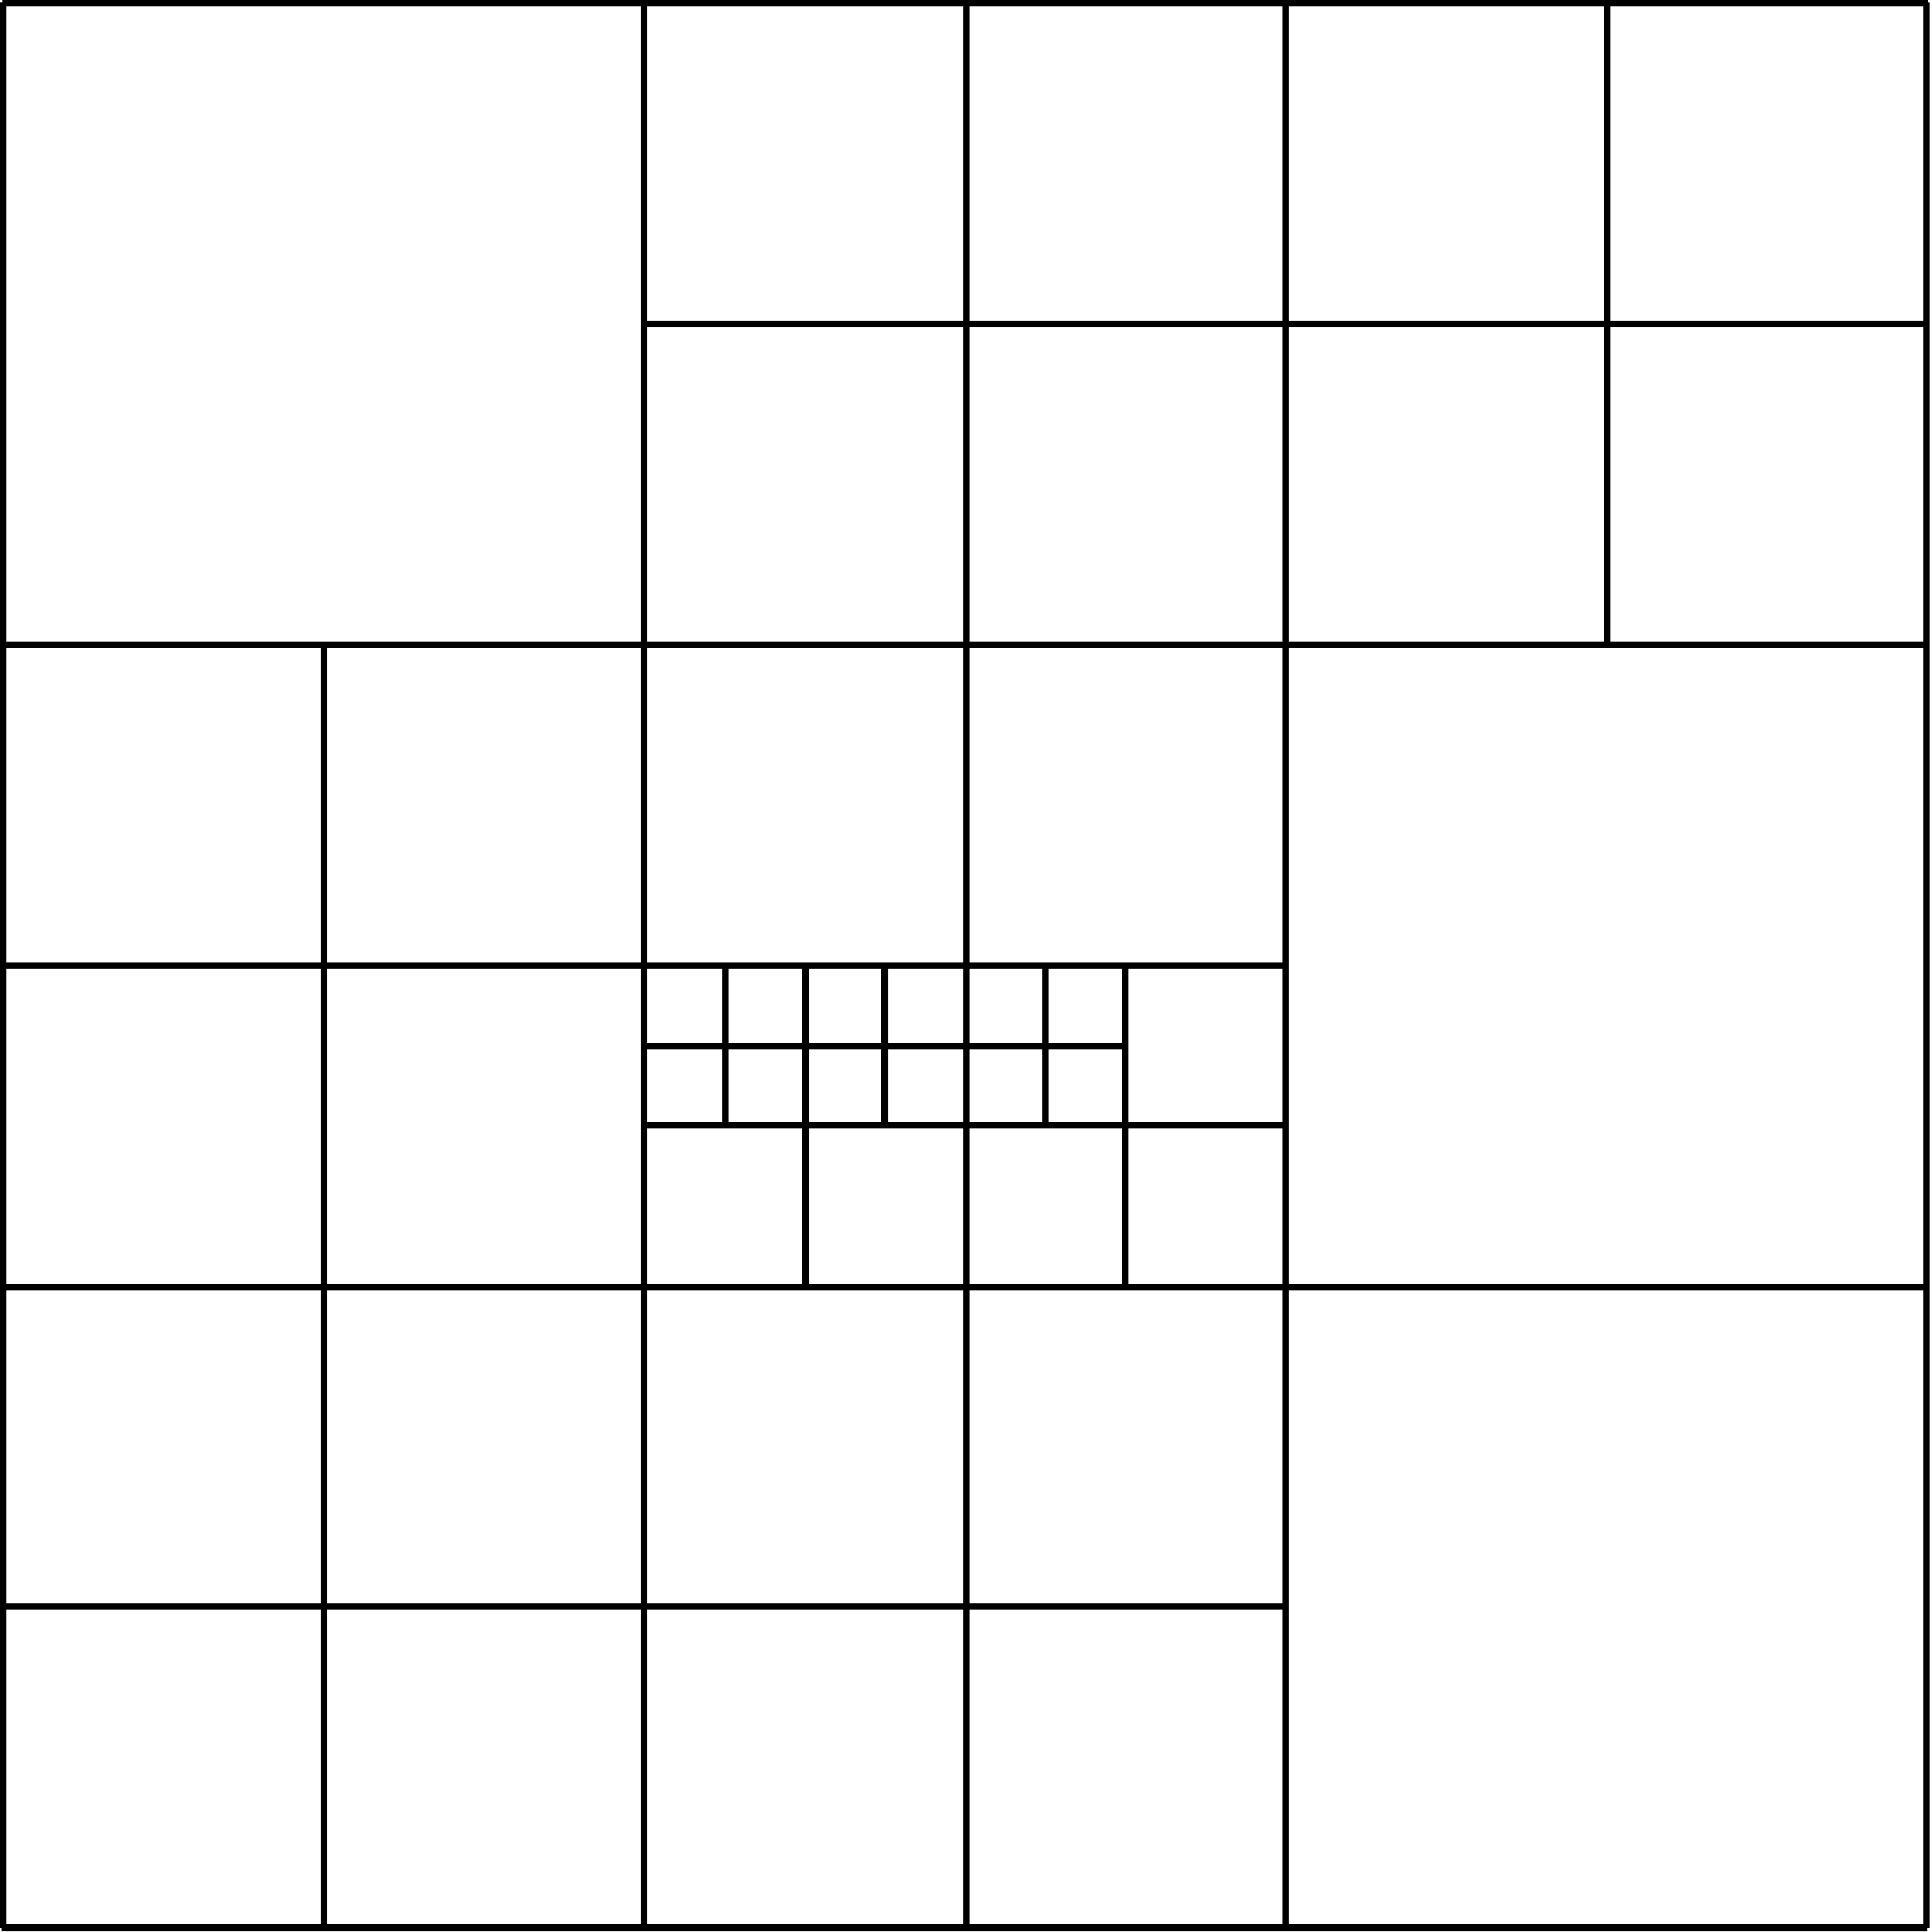
\includegraphics[width=.6\textwidth]{Images/Figure 1.pdf}};
    \begin{scope}[x={(image.south east)},y={(image.north west)}]
    \begin{scope}[x={(image.south east)},y={(image.north west)}]
        \node at (0.165,0.83) {\tiny U};
        \node at (0.42,0.915) {\tiny V};
        \node at (0.58,0.915) {\tiny V};
        \node at (0.75,0.915) {\tiny V};
        \node at (0.91,0.915) {\tiny V};
        \node at (0.42,0.75) {\tiny U};
        \node at (0.58,0.75) {\tiny U};
        \node at (0.75,0.75) {\tiny V};
        \node at (0.91,0.75) {\tiny V};
        \node at (0.08,0.58) {\tiny V};
        \node at (0.25,0.58) {\tiny U};
        \node at (0.42,0.58) {\tiny {\color{red} B}};
        \node at (0.58,0.58) {\tiny U};
        \node at (0.83,0.5) {\tiny X};
        \node at (0.08,0.42) {\tiny V};
        \node at (0.25,0.42) {\tiny U};
        \node at (0.355,0.48) {\tiny U};
        \node at (0.40,0.48) {\tiny U};
        \node at (0.44,0.48) {\tiny U};
        \node at (0.48,0.48) {\tiny U};
        \node at (0.52,0.48) {\tiny U};
        \node at (0.56,0.48) {\tiny W};
        \node at (0.62,0.46) {\tiny W};
        \node at (0.355,0.44) {\tiny W};
        \node at (0.40,0.44) {\tiny W};
        \node at (0.44,0.44) {\tiny W};
        \node at (0.48,0.44) {\tiny W};
        \node at (0.52,0.44) {\tiny W};
        \node at (0.56,0.44) {\tiny W};
        \node at (0.38,0.38) {\tiny W};
        \node at (0.46,0.38) {\tiny W};
        \node at (0.54,0.38) {\tiny W};
        \node at (0.62,0.38) {\tiny W};        
        \node at (0.08,0.25) {\tiny V};
        \node at (0.25,0.25) {\tiny V};
        \node at (0.42,0.25) {\tiny V};
        \node at (0.58,0.25) {\tiny V};
        \node at (0.83,0.16) {\tiny X};
        \node at (0.08,0.08) {\tiny V};
        \node at (0.25,0.08) {\tiny V};
        \node at (0.42,0.08) {\tiny V};
        \node at (0.58,0.08) {\tiny V};
    \end{scope}
    \end{scope}
\end{tikzpicture}
    \caption{A 2D example of the interaction lists $I_U^B, I_V^B, I_X^B$ and $I_W^B$ for a node $B$}
    \label{fig:InteractionsLists}
\end{figure}


In the figure \ref{fig:InteractionsLists} we show the 2D interactions list for a node $B$ for a random arrangement of nodes, note that these might not all be leaf nodes. These lists contain all the nodes from which we need to consider the contributions as well as the node's parent. In order to see how these nodes interact with each other, we will define the near and far-field of each node. We will denote the near field of a node $B$ to be $\mathcal{N}(B)$ which is the set of all nodes in $I_U^B$ and $I_X^B$, and the far-field $\mathcal{F}(B)$ to be all remaining nodes. While geometrically these definitions may be convoluted with nodes in the far-field being geometrically closer than those in the near field they provide definitions for which nodes need to be computed directly or through the use of equivalent surfaces.

\subsection{Equivalent surfaces}

The KIFMM makes use of two equivalent surfaces for each node in the Octree to approximate the effect between source and source points inside and outside the node. The upwards equivalent surface is taken to be the boundary of the node $B$ (denoted $\Omega^U$) and the downwards equivalent surface to be the surface of a cube of width three times larger and centred on the node $B$ (denoted $\Omega^D$) as illustrated in \cref{fig:UpandDownsurf} \cite{Ying2004}. Upon both of these surfaces we denote equivalent potential densities $\bm{f}^{BU}$ and $\bm{f}^{BD}$ for the upwards and downwards equivalent surface's of $B$ respectively. The upward equivalent surface is used to approximate the effect of all source points contained within the node and its decedents \cite{Rostami2016Kernel-independentStokeslets}. As such we can say that for every point $\bm{x}\in\mathcal{F}(B)$ the velocity induced by that of the equivalent surface is the same as that induced by all source points in $B$, this gives us
\begin{equation}
\label{eq:upsurfint}
    \forall \;\bm{x} \in \mathcal{F}(B): \quad \int_{\Omega^U} S^\epsilon(\bm{x}, \bm{y}) \bm{f}^{BU}(\bm{y}) d \bm{y}=\sum_{{\bm{y}}_n \in B} S^\epsilon\left(\bm{x}, {\bm{y}}_n\right) {\bm{f}}_{n}
\end{equation}

The same can be applied to the downwards equivalent surface where instead the contributions are obtained from source points in $\mathcal{F}(B)$, we can say that for any point in $B$ the velocity induced by the downwards surface equals that induced by the source points in $\mathcal{F}(B)$, which again gives us that
\begin{equation}
\label{eq:downsurfint}
    \forall \;\bm{x} \in B: \quad \int_{\Omega^D} S^\epsilon(\bm{x}, \bm{y}) \bm{f}^{BD}(\bm{y}) d \bm{y}=\sum_{{\bm{y}}_n \in \mathcal{F}(B)} S^\epsilon\left(\bm{x}, {\bm{y}}_n\right) {\bm{f}}_{n}
\end{equation}

\begin{figure}[ht]
    \centering
    \resizebox{.6\linewidth}{!}{% This file was created by matlab2tikz.
%
%The latest updates can be retrieved from
%  http://www.mathworks.com/matlabcentral/fileexchange/22022-matlab2tikz-matlab2tikz
%where you can also make suggestions and rate matlab2tikz.
%
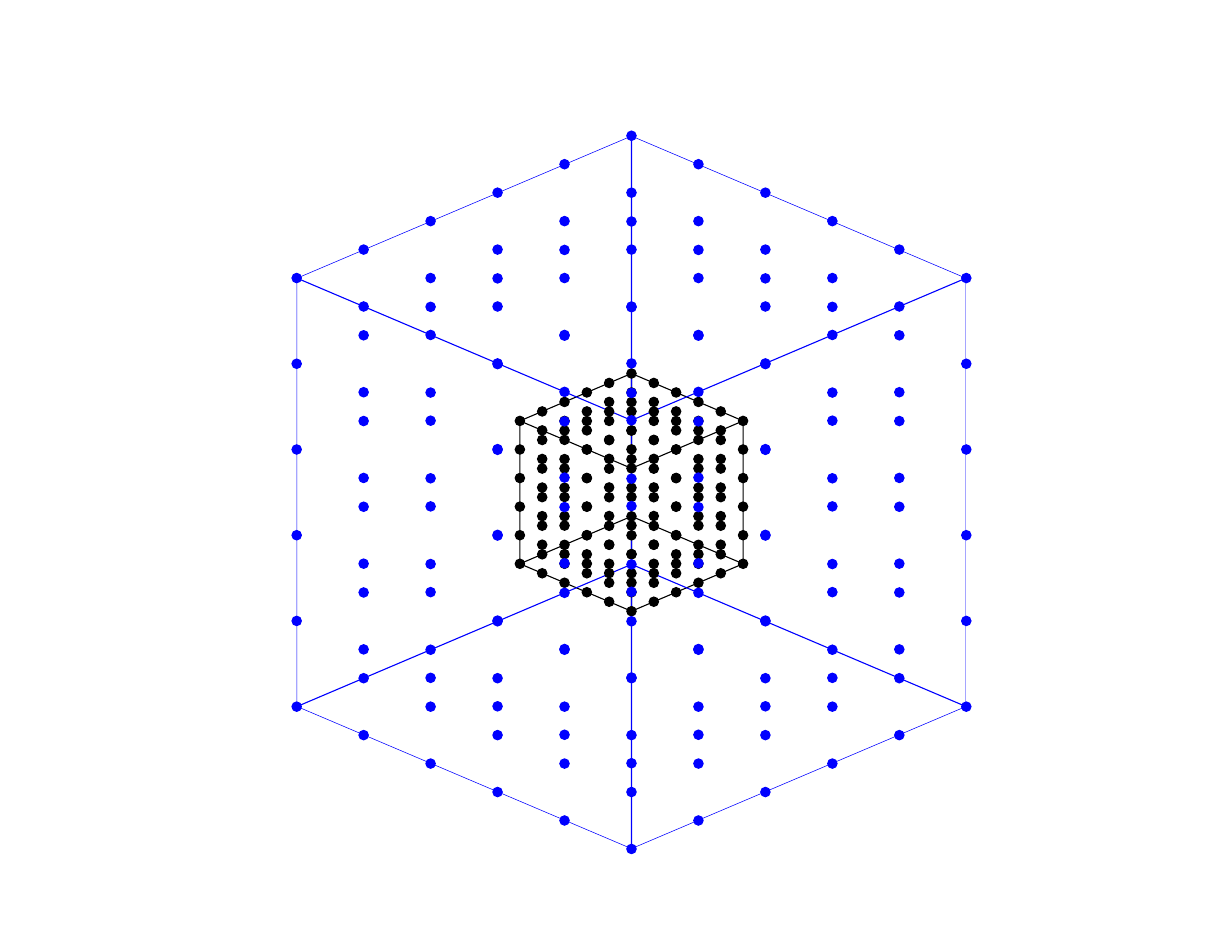
\begin{tikzpicture}

\begin{axis}[%
width=3.348in,
height=3.566in,
at={(1.345in,0.481in)},
scale only axis,
plot box ratio=1 1 1,
unbounded coords=jump,
xmin=-0.793615595547456,
xmax=1.67889551819639,
tick align=outside,
ymin=-0.793615595547456,
ymax=1.67889551819639,
zmin=-0.793615595547456,
zmax=1.67889551819639,
view={45}{25.15},
axis line style={draw=none},
ticks=none,
axis x line*=bottom,
axis y line*=left,
axis z line*=left
]
\addplot3 [color=black, only marks, mark size=1.7pt, mark=*, mark options={solid, black}]
 table[row sep=crcr] {%
0.0305547757004935	0.0305547757004935	0.0305547757004935\\
0.0305547757004935	0.195388849950083	0.0305547757004935\\
0.0305547757004935	0.360222924199673	0.0305547757004935\\
0.0305547757004935	0.525056998449263	0.0305547757004935\\
0.0305547757004935	0.689891072698853	0.0305547757004935\\
0.0305547757004935	0.854725146948443	0.0305547757004935\\
0.195388849950083	0.0305547757004935	0.0305547757004935\\
0.195388849950083	0.195388849950083	0.0305547757004935\\
0.195388849950083	0.360222924199673	0.0305547757004935\\
0.195388849950083	0.525056998449263	0.0305547757004935\\
0.195388849950083	0.689891072698853	0.0305547757004935\\
0.195388849950083	0.854725146948443	0.0305547757004935\\
0.360222924199673	0.0305547757004935	0.0305547757004935\\
0.360222924199673	0.195388849950083	0.0305547757004935\\
0.360222924199673	0.360222924199673	0.0305547757004935\\
0.360222924199673	0.525056998449263	0.0305547757004935\\
0.360222924199673	0.689891072698853	0.0305547757004935\\
0.360222924199673	0.854725146948443	0.0305547757004935\\
0.525056998449263	0.0305547757004935	0.0305547757004935\\
0.525056998449263	0.195388849950083	0.0305547757004935\\
0.525056998449263	0.360222924199673	0.0305547757004935\\
0.525056998449263	0.525056998449263	0.0305547757004935\\
0.525056998449263	0.689891072698853	0.0305547757004935\\
0.525056998449263	0.854725146948443	0.0305547757004935\\
0.689891072698853	0.0305547757004935	0.0305547757004935\\
0.689891072698853	0.195388849950083	0.0305547757004935\\
0.689891072698853	0.360222924199673	0.0305547757004935\\
0.689891072698853	0.525056998449263	0.0305547757004935\\
0.689891072698853	0.689891072698853	0.0305547757004935\\
0.689891072698853	0.854725146948443	0.0305547757004935\\
0.854725146948443	0.0305547757004935	0.0305547757004935\\
0.854725146948443	0.195388849950083	0.0305547757004935\\
0.854725146948443	0.360222924199673	0.0305547757004935\\
0.854725146948443	0.525056998449263	0.0305547757004935\\
0.854725146948443	0.689891072698853	0.0305547757004935\\
0.854725146948443	0.854725146948443	0.0305547757004935\\
0.0305547757004935	0.0305547757004935	0.195388849950083\\
0.0305547757004935	0.195388849950083	0.195388849950083\\
0.0305547757004935	0.360222924199673	0.195388849950083\\
0.0305547757004935	0.525056998449263	0.195388849950083\\
0.0305547757004935	0.689891072698853	0.195388849950083\\
0.0305547757004935	0.854725146948443	0.195388849950083\\
0.195388849950083	0.0305547757004935	0.195388849950083\\
0.195388849950083	0.854725146948443	0.195388849950083\\
0.360222924199673	0.0305547757004935	0.195388849950083\\
0.360222924199673	0.854725146948443	0.195388849950083\\
0.525056998449263	0.0305547757004935	0.195388849950083\\
0.525056998449263	0.854725146948443	0.195388849950083\\
0.689891072698853	0.0305547757004935	0.195388849950083\\
0.689891072698853	0.854725146948443	0.195388849950083\\
0.854725146948443	0.0305547757004935	0.195388849950083\\
0.854725146948443	0.195388849950083	0.195388849950083\\
0.854725146948443	0.360222924199673	0.195388849950083\\
0.854725146948443	0.525056998449263	0.195388849950083\\
0.854725146948443	0.689891072698853	0.195388849950083\\
0.854725146948443	0.854725146948443	0.195388849950083\\
0.0305547757004935	0.0305547757004935	0.360222924199673\\
0.0305547757004935	0.195388849950083	0.360222924199673\\
0.0305547757004935	0.360222924199673	0.360222924199673\\
0.0305547757004935	0.525056998449263	0.360222924199673\\
0.0305547757004935	0.689891072698853	0.360222924199673\\
0.0305547757004935	0.854725146948443	0.360222924199673\\
0.195388849950083	0.0305547757004935	0.360222924199673\\
0.195388849950083	0.854725146948443	0.360222924199673\\
0.360222924199673	0.0305547757004935	0.360222924199673\\
0.360222924199673	0.854725146948443	0.360222924199673\\
0.525056998449263	0.0305547757004935	0.360222924199673\\
0.525056998449263	0.854725146948443	0.360222924199673\\
0.689891072698853	0.0305547757004935	0.360222924199673\\
0.689891072698853	0.854725146948443	0.360222924199673\\
0.854725146948443	0.0305547757004935	0.360222924199673\\
0.854725146948443	0.195388849950083	0.360222924199673\\
0.854725146948443	0.360222924199673	0.360222924199673\\
0.854725146948443	0.525056998449263	0.360222924199673\\
0.854725146948443	0.689891072698853	0.360222924199673\\
0.854725146948443	0.854725146948443	0.360222924199673\\
0.0305547757004935	0.0305547757004935	0.525056998449263\\
0.0305547757004935	0.195388849950083	0.525056998449263\\
0.0305547757004935	0.360222924199673	0.525056998449263\\
0.0305547757004935	0.525056998449263	0.525056998449263\\
0.0305547757004935	0.689891072698853	0.525056998449263\\
0.0305547757004935	0.854725146948443	0.525056998449263\\
0.195388849950083	0.0305547757004935	0.525056998449263\\
0.195388849950083	0.854725146948443	0.525056998449263\\
0.360222924199673	0.0305547757004935	0.525056998449263\\
0.360222924199673	0.854725146948443	0.525056998449263\\
0.525056998449263	0.0305547757004935	0.525056998449263\\
0.525056998449263	0.854725146948443	0.525056998449263\\
0.689891072698853	0.0305547757004935	0.525056998449263\\
0.689891072698853	0.854725146948443	0.525056998449263\\
0.854725146948443	0.0305547757004935	0.525056998449263\\
0.854725146948443	0.195388849950083	0.525056998449263\\
0.854725146948443	0.360222924199673	0.525056998449263\\
0.854725146948443	0.525056998449263	0.525056998449263\\
0.854725146948443	0.689891072698853	0.525056998449263\\
0.854725146948443	0.854725146948443	0.525056998449263\\
0.0305547757004935	0.0305547757004935	0.689891072698853\\
0.0305547757004935	0.195388849950083	0.689891072698853\\
0.0305547757004935	0.360222924199673	0.689891072698853\\
0.0305547757004935	0.525056998449263	0.689891072698853\\
0.0305547757004935	0.689891072698853	0.689891072698853\\
0.0305547757004935	0.854725146948443	0.689891072698853\\
0.195388849950083	0.0305547757004935	0.689891072698853\\
0.195388849950083	0.854725146948443	0.689891072698853\\
0.360222924199673	0.0305547757004935	0.689891072698853\\
0.360222924199673	0.854725146948443	0.689891072698853\\
0.525056998449263	0.0305547757004935	0.689891072698853\\
0.525056998449263	0.854725146948443	0.689891072698853\\
0.689891072698853	0.0305547757004935	0.689891072698853\\
0.689891072698853	0.854725146948443	0.689891072698853\\
0.854725146948443	0.0305547757004935	0.689891072698853\\
0.854725146948443	0.195388849950083	0.689891072698853\\
0.854725146948443	0.360222924199673	0.689891072698853\\
0.854725146948443	0.525056998449263	0.689891072698853\\
0.854725146948443	0.689891072698853	0.689891072698853\\
0.854725146948443	0.854725146948443	0.689891072698853\\
0.0305547757004935	0.0305547757004935	0.854725146948443\\
0.0305547757004935	0.195388849950083	0.854725146948443\\
0.0305547757004935	0.360222924199673	0.854725146948443\\
0.0305547757004935	0.525056998449263	0.854725146948443\\
0.0305547757004935	0.689891072698853	0.854725146948443\\
0.0305547757004935	0.854725146948443	0.854725146948443\\
0.195388849950083	0.0305547757004935	0.854725146948443\\
0.195388849950083	0.195388849950083	0.854725146948443\\
0.195388849950083	0.360222924199673	0.854725146948443\\
0.195388849950083	0.525056998449263	0.854725146948443\\
0.195388849950083	0.689891072698853	0.854725146948443\\
0.195388849950083	0.854725146948443	0.854725146948443\\
0.360222924199673	0.0305547757004935	0.854725146948443\\
0.360222924199673	0.195388849950083	0.854725146948443\\
0.360222924199673	0.360222924199673	0.854725146948443\\
0.360222924199673	0.525056998449263	0.854725146948443\\
0.360222924199673	0.689891072698853	0.854725146948443\\
0.360222924199673	0.854725146948443	0.854725146948443\\
0.525056998449263	0.0305547757004935	0.854725146948443\\
0.525056998449263	0.195388849950083	0.854725146948443\\
0.525056998449263	0.360222924199673	0.854725146948443\\
0.525056998449263	0.525056998449263	0.854725146948443\\
0.525056998449263	0.689891072698853	0.854725146948443\\
0.525056998449263	0.854725146948443	0.854725146948443\\
0.689891072698853	0.0305547757004935	0.854725146948443\\
0.689891072698853	0.195388849950083	0.854725146948443\\
0.689891072698853	0.360222924199673	0.854725146948443\\
0.689891072698853	0.525056998449263	0.854725146948443\\
0.689891072698853	0.689891072698853	0.854725146948443\\
0.689891072698853	0.854725146948443	0.854725146948443\\
0.854725146948443	0.0305547757004935	0.854725146948443\\
0.854725146948443	0.195388849950083	0.854725146948443\\
0.854725146948443	0.360222924199673	0.854725146948443\\
0.854725146948443	0.525056998449263	0.854725146948443\\
0.854725146948443	0.689891072698853	0.854725146948443\\
0.854725146948443	0.854725146948443	0.854725146948443\\
};
 \addplot3 [color=blue, only marks, mark size=1.7pt, mark=*, mark options={solid, blue}]
 table[row sep=crcr] {%
-0.793615595547456	-0.793615595547456	-0.793615595547456\\
-0.793615595547456	-0.299113372798686	-0.793615595547456\\
-0.793615595547456	0.195388849950083	-0.793615595547456\\
-0.793615595547456	0.689891072698853	-0.793615595547456\\
-0.793615595547456	1.18439329544762	-0.793615595547456\\
-0.793615595547456	1.67889551819639	-0.793615595547456\\
-0.299113372798686	-0.793615595547456	-0.793615595547456\\
-0.299113372798686	-0.299113372798686	-0.793615595547456\\
-0.299113372798686	0.195388849950083	-0.793615595547456\\
-0.299113372798686	0.689891072698853	-0.793615595547456\\
-0.299113372798686	1.18439329544762	-0.793615595547456\\
-0.299113372798686	1.67889551819639	-0.793615595547456\\
0.195388849950083	-0.793615595547456	-0.793615595547456\\
0.195388849950083	-0.299113372798686	-0.793615595547456\\
0.195388849950083	0.195388849950083	-0.793615595547456\\
0.195388849950083	0.689891072698853	-0.793615595547456\\
0.195388849950083	1.18439329544762	-0.793615595547456\\
0.195388849950083	1.67889551819639	-0.793615595547456\\
0.689891072698853	-0.793615595547456	-0.793615595547456\\
0.689891072698853	-0.299113372798686	-0.793615595547456\\
0.689891072698853	0.195388849950083	-0.793615595547456\\
0.689891072698853	0.689891072698853	-0.793615595547456\\
0.689891072698853	1.18439329544762	-0.793615595547456\\
0.689891072698853	1.67889551819639	-0.793615595547456\\
1.18439329544762	-0.793615595547456	-0.793615595547456\\
1.18439329544762	-0.299113372798686	-0.793615595547456\\
1.18439329544762	0.195388849950083	-0.793615595547456\\
1.18439329544762	0.689891072698853	-0.793615595547456\\
1.18439329544762	1.18439329544762	-0.793615595547456\\
1.18439329544762	1.67889551819639	-0.793615595547456\\
1.67889551819639	-0.793615595547456	-0.793615595547456\\
1.67889551819639	-0.299113372798686	-0.793615595547456\\
1.67889551819639	0.195388849950083	-0.793615595547456\\
1.67889551819639	0.689891072698853	-0.793615595547456\\
1.67889551819639	1.18439329544762	-0.793615595547456\\
1.67889551819639	1.67889551819639	-0.793615595547456\\
-0.793615595547456	-0.793615595547456	-0.299113372798686\\
-0.793615595547456	-0.299113372798686	-0.299113372798686\\
-0.793615595547456	0.195388849950083	-0.299113372798686\\
-0.793615595547456	0.689891072698853	-0.299113372798686\\
-0.793615595547456	1.18439329544762	-0.299113372798686\\
-0.793615595547456	1.67889551819639	-0.299113372798686\\
-0.299113372798686	-0.793615595547456	-0.299113372798686\\
-0.299113372798686	1.67889551819639	-0.299113372798686\\
0.195388849950083	-0.793615595547456	-0.299113372798686\\
0.195388849950083	1.67889551819639	-0.299113372798686\\
0.689891072698853	-0.793615595547456	-0.299113372798686\\
0.689891072698853	1.67889551819639	-0.299113372798686\\
1.18439329544762	-0.793615595547456	-0.299113372798686\\
1.18439329544762	1.67889551819639	-0.299113372798686\\
1.67889551819639	-0.793615595547456	-0.299113372798686\\
1.67889551819639	-0.299113372798686	-0.299113372798686\\
1.67889551819639	0.195388849950083	-0.299113372798686\\
1.67889551819639	0.689891072698853	-0.299113372798686\\
1.67889551819639	1.18439329544762	-0.299113372798686\\
1.67889551819639	1.67889551819639	-0.299113372798686\\
-0.793615595547456	-0.793615595547456	0.195388849950083\\
-0.793615595547456	-0.299113372798686	0.195388849950083\\
-0.793615595547456	0.195388849950083	0.195388849950083\\
-0.793615595547456	0.689891072698853	0.195388849950083\\
-0.793615595547456	1.18439329544762	0.195388849950083\\
-0.793615595547456	1.67889551819639	0.195388849950083\\
-0.299113372798686	-0.793615595547456	0.195388849950083\\
-0.299113372798686	1.67889551819639	0.195388849950083\\
0.195388849950083	-0.793615595547456	0.195388849950083\\
0.195388849950083	1.67889551819639	0.195388849950083\\
0.689891072698853	-0.793615595547456	0.195388849950083\\
0.689891072698853	1.67889551819639	0.195388849950083\\
1.18439329544762	-0.793615595547456	0.195388849950083\\
1.18439329544762	1.67889551819639	0.195388849950083\\
1.67889551819639	-0.793615595547456	0.195388849950083\\
1.67889551819639	-0.299113372798686	0.195388849950083\\
1.67889551819639	0.195388849950083	0.195388849950083\\
1.67889551819639	0.689891072698853	0.195388849950083\\
1.67889551819639	1.18439329544762	0.195388849950083\\
1.67889551819639	1.67889551819639	0.195388849950083\\
-0.793615595547456	-0.793615595547456	0.689891072698853\\
-0.793615595547456	-0.299113372798686	0.689891072698853\\
-0.793615595547456	0.195388849950083	0.689891072698853\\
-0.793615595547456	0.689891072698853	0.689891072698853\\
-0.793615595547456	1.18439329544762	0.689891072698853\\
-0.793615595547456	1.67889551819639	0.689891072698853\\
-0.299113372798686	-0.793615595547456	0.689891072698853\\
-0.299113372798686	1.67889551819639	0.689891072698853\\
0.195388849950083	-0.793615595547456	0.689891072698853\\
0.195388849950083	1.67889551819639	0.689891072698853\\
0.689891072698853	-0.793615595547456	0.689891072698853\\
0.689891072698853	1.67889551819639	0.689891072698853\\
1.18439329544762	-0.793615595547456	0.689891072698853\\
1.18439329544762	1.67889551819639	0.689891072698853\\
1.67889551819639	-0.793615595547456	0.689891072698853\\
1.67889551819639	-0.299113372798686	0.689891072698853\\
1.67889551819639	0.195388849950083	0.689891072698853\\
1.67889551819639	0.689891072698853	0.689891072698853\\
1.67889551819639	1.18439329544762	0.689891072698853\\
1.67889551819639	1.67889551819639	0.689891072698853\\
-0.793615595547456	-0.793615595547456	1.18439329544762\\
-0.793615595547456	-0.299113372798686	1.18439329544762\\
-0.793615595547456	0.195388849950083	1.18439329544762\\
-0.793615595547456	0.689891072698853	1.18439329544762\\
-0.793615595547456	1.18439329544762	1.18439329544762\\
-0.793615595547456	1.67889551819639	1.18439329544762\\
-0.299113372798686	-0.793615595547456	1.18439329544762\\
-0.299113372798686	1.67889551819639	1.18439329544762\\
0.195388849950083	-0.793615595547456	1.18439329544762\\
0.195388849950083	1.67889551819639	1.18439329544762\\
0.689891072698853	-0.793615595547456	1.18439329544762\\
0.689891072698853	1.67889551819639	1.18439329544762\\
1.18439329544762	-0.793615595547456	1.18439329544762\\
1.18439329544762	1.67889551819639	1.18439329544762\\
1.67889551819639	-0.793615595547456	1.18439329544762\\
1.67889551819639	-0.299113372798686	1.18439329544762\\
1.67889551819639	0.195388849950083	1.18439329544762\\
1.67889551819639	0.689891072698853	1.18439329544762\\
1.67889551819639	1.18439329544762	1.18439329544762\\
1.67889551819639	1.67889551819639	1.18439329544762\\
-0.793615595547456	-0.793615595547456	1.67889551819639\\
-0.793615595547456	-0.299113372798686	1.67889551819639\\
-0.793615595547456	0.195388849950083	1.67889551819639\\
-0.793615595547456	0.689891072698853	1.67889551819639\\
-0.793615595547456	1.18439329544762	1.67889551819639\\
-0.793615595547456	1.67889551819639	1.67889551819639\\
-0.299113372798686	-0.793615595547456	1.67889551819639\\
-0.299113372798686	-0.299113372798686	1.67889551819639\\
-0.299113372798686	0.195388849950083	1.67889551819639\\
-0.299113372798686	0.689891072698853	1.67889551819639\\
-0.299113372798686	1.18439329544762	1.67889551819639\\
-0.299113372798686	1.67889551819639	1.67889551819639\\
0.195388849950083	-0.793615595547456	1.67889551819639\\
0.195388849950083	-0.299113372798686	1.67889551819639\\
0.195388849950083	0.195388849950083	1.67889551819639\\
0.195388849950083	0.689891072698853	1.67889551819639\\
0.195388849950083	1.18439329544762	1.67889551819639\\
0.195388849950083	1.67889551819639	1.67889551819639\\
0.689891072698853	-0.793615595547456	1.67889551819639\\
0.689891072698853	-0.299113372798686	1.67889551819639\\
0.689891072698853	0.195388849950083	1.67889551819639\\
0.689891072698853	0.689891072698853	1.67889551819639\\
0.689891072698853	1.18439329544762	1.67889551819639\\
0.689891072698853	1.67889551819639	1.67889551819639\\
1.18439329544762	-0.793615595547456	1.67889551819639\\
1.18439329544762	-0.299113372798686	1.67889551819639\\
1.18439329544762	0.195388849950083	1.67889551819639\\
1.18439329544762	0.689891072698853	1.67889551819639\\
1.18439329544762	1.18439329544762	1.67889551819639\\
1.18439329544762	1.67889551819639	1.67889551819639\\
1.67889551819639	-0.793615595547456	1.67889551819639\\
1.67889551819639	-0.299113372798686	1.67889551819639\\
1.67889551819639	0.195388849950083	1.67889551819639\\
1.67889551819639	0.689891072698853	1.67889551819639\\
1.67889551819639	1.18439329544762	1.67889551819639\\
1.67889551819639	1.67889551819639	1.67889551819639\\
};
 \addplot3 [color=black]
 table[row sep=crcr] {%
0.0305547757004935	0.0305547757004935	0.0305547757004935\\
0.854725146948443	0.0305547757004935	0.0305547757004935\\
0.854725146948443	0.854725146948443	0.0305547757004935\\
0.0305547757004935	0.854725146948443	0.0305547757004935\\
0.0305547757004935	0.0305547757004935	0.0305547757004935\\
0.0305547757004935	0.0305547757004935	0.854725146948443\\
0.854725146948443	0.0305547757004935	0.854725146948443\\
0.854725146948443	0.854725146948443	0.854725146948443\\
0.0305547757004935	0.854725146948443	0.854725146948443\\
0.0305547757004935	0.0305547757004935	0.854725146948443\\
0.0305547757004935	0.0305547757004935	0.0305547757004935\\
nan	nan	nan\\
0.854725146948443	0.0305547757004935	0.0305547757004935\\
0.854725146948443	0.0305547757004935	0.854725146948443\\
nan	nan	nan\\
0.854725146948443	0.854725146948443	0.0305547757004935\\
0.854725146948443	0.854725146948443	0.854725146948443\\
nan	nan	nan\\
0.0305547757004935	0.854725146948443	0.0305547757004935\\
0.0305547757004935	0.854725146948443	0.854725146948443\\
};
 \addplot3 [color=blue]
 table[row sep=crcr] {%
-0.793615595547456	-0.793615595547456	-0.793615595547456\\
1.67889551819639	-0.793615595547456	-0.793615595547456\\
1.67889551819639	1.67889551819639	-0.793615595547456\\
-0.793615595547456	1.67889551819639	-0.793615595547456\\
-0.793615595547456	-0.793615595547456	-0.793615595547456\\
-0.793615595547456	-0.793615595547456	1.67889551819639\\
1.67889551819639	-0.793615595547456	1.67889551819639\\
1.67889551819639	1.67889551819639	1.67889551819639\\
-0.793615595547456	1.67889551819639	1.67889551819639\\
-0.793615595547456	-0.793615595547456	1.67889551819639\\
-0.793615595547456	-0.793615595547456	-0.793615595547456\\
nan	nan	nan\\
1.67889551819639	-0.793615595547456	-0.793615595547456\\
1.67889551819639	-0.793615595547456	1.67889551819639\\
nan	nan	nan\\
1.67889551819639	1.67889551819639	-0.793615595547456\\
1.67889551819639	1.67889551819639	1.67889551819639\\
nan	nan	nan\\
-0.793615595547456	1.67889551819639	-0.793615595547456\\
-0.793615595547456	1.67889551819639	1.67889551819639\\
};
 \end{axis}

\begin{axis}[%
width=5.833in,
height=4.375in,
at={(0in,0in)},
scale only axis,
xmin=0,
xmax=1,
ymin=0,
ymax=1,
axis line style={draw=none},
ticks=none,
axis x line*=bottom,
axis y line*=left
]
\end{axis}
\end{tikzpicture}%}
    \caption{A diagram representing the upwards and downwards equivalent surface for an arbitrary node with bounds given in black. Both surfaces are discredited by a $6 \times 6 \times 6$ set of quadrature points. The upwards equivalent surface (black) lies on the boundary of the node while the downward equivalent surface (blue) is a cube with sides 3 times larger and centred on the node. }
    \label{fig:UpandDownsurf}
\end{figure}

In order to be able to use these equivalent potentials densities in our method, we form a quadrature rule over an equally spaced uniform Cartesian grid with $N_q$ quadrature point. While the number of quadrature points in the upwards and downwards equivalent surfaces does not need to be the same, for convenience we will take this to be the case. We will indicate the quadrature points the upwards equivalent potential for a node $B$ with $\{\bm{q}^{BU}_m\}$ for $m=1,\dots,N_q$ and $\{\bm{q}^{BD}_m\}$ for $m=1,\dots,N_q$ indicating the positions of the quadrature points for the downwards equivalent potential. Now each of these quadrature points has a corresponding equivalent potential denoted by $\{\bm{f}^{BU}(\bm{q}^{BU}_m)\}$ and $\{\bm{f}^{BD}(\bm{q}^{BD}_m)\}$ for the upward and downward equivalent potentials respectively. Writing the left-hand side of \cref{eq:upsurfint,eq:downsurfint} using this quadrature rule we obtain that
\begin{equation}
\label{eq:L2Mfar}
    \forall \;\bm{x} \in \mathcal{F}(B): \quad \bm{u}(\bm{x})= \frac{1}{8 \pi \mu} \sum_{m=1}^{N_{q}} A_{m}^{BU} S^\epsilon\left(\bm{x}, \bm{q}_{m}^{B U}\right) \bm{f}^{B U}\left(\bm{q}_{m}^{B U}\right)
\end{equation}
and the contribution to the velocity $\bm{u}(\bm{x})$ for $\bm{x} \in B$ from source points in $\mathcal{F}(B)$ as
\begin{equation}
\label{eq:L2Mnear}
    \forall \;\bm{x} \in B: \quad \bm{u}(\bm{x})= \frac{1}{8 \pi \mu} \sum_{m=1}^{N_{q}} A_{m}^{BD} S^\epsilon\left(\bm{x}, \bm{q}_{m}^{B D}\right) \bm{f}^{B D}\left(\bm{q}_{m}^{B D}\right)
\end{equation}
Where $\{A_{m}^{BU}\}$ and $\{A_{m}^{BD}\}$ are the corresponding quadrature weights of the upwards and downward equivalent points respectively. We will not explicitly calculate these weights and will take them to be part of their corresponding equivalent potential. The advantage of using \cref{eq:L2Mnear,eq:L2Mfar} is to avoid the direct computation of source points and target points and instead use the quadrature points as an approximation of the particles within the box.

We note that the downward equivalent surface lies in the $\mathcal{F}(B)$ and the downward equivalent surface lies in $B$ and hence we obtain the following systems of equations
\begin{equation}
\label{eq:upsum}
    \sum_{m=1}^{N_{q}} A_{m}^{BU} S^\epsilon\left(\bm{q}^{BD}_{k}, \bm{q}_{m}^{B U}\right) \bm{f}^{B U}\left(\bm{q}_{m}^{B U}\right)=\sum_{{\bm{y}}_{n} \in B} S^\epsilon\left(\bm{q}^{BD}_{k}, {\bm{y}}_{n}\right) {\bm{f}}_{n} A({\bm{y}}_n), \quad k=1,\dots,N_q
\end{equation}
and
\begin{equation}
\label{eq:downsum}
    \sum_{m=1}^{N_{q}} A_{m}^{BD} S^\epsilon\left(\bm{q}^{BU}_{k}, \bm{q}_{m}^{B D}\right) \bm{f}^{B D}\left(\bm{q}_{m}^{B D}\right)=\sum_{{\bm{y}}_{n} \in \mathcal{F}(B)} S^\epsilon\left(\bm{q}^{BU}_{k}, {\bm{y}}_{n}\right) {\bm{f}}_{n} A({\bm{y}}_n), \quad k=1,\dots,N_q
\end{equation}
We will use \cref{eq:upsum,eq:downsum} to construct the upwards and downwards potential of all nodes through the approximation the left-hand sides of the equation. 

\subsection{Evaluation}
The Fast Multipole method is based on two passes, one up the tree in order to construct the upwards equivalent surfaces from source potentials and a further downward pass where we construct the downward equivalent potentials before finally evaluating the velocities at the target points. 

\subsubsection{Upward Pass}
The upwards pass involves the postorder traversal of the tree from the smallest node up to the root node and solving \cref{eq:upsum} for each node. For each leaf node, we can evaluate the right-hand side of \cref{eq:upsum} directly. Now for each non-leaf node $B$ in the tree instead of summing over all source points in the decedents of $B$ we can approximate its upwards equivalent surface from its children. We denote the children of $B$ as $C_l^B$ where $l=1,...,8$. As we have traversed the tree in post-order we know $\{\bm{f}^{C_l U}(\bm{q}^{C_lU}_m)\}$ for $l=1,\dots,8$ and $m=1,\dots,N_q$. Since $\{\bm{q}^{C_lU}_m\}$ lies within $\{\bm{q}^{BU}_m\}$ we have that the right-hand side of \cref{eq:upsum} can be approximated as 
\begin{equation}
\label{eq:M2M}
    \sum_{l=1}^{8} \sum_{m=1}^{N_{q}} A_{m}^{C_{l} U} S^\epsilon\left(\bm{q}_{k}^{B D}, \bm{q}_{m}^{C_{l} U}\right) \bm{f}^{C_{l} U}\left(\bm{q}_{m}^{C_{l} U}\right), \quad k=1,\dots,N_q
\end{equation}
We refer to this as a multipole to multipole translation (M2M). This method of approximating the parents equivalent potential from its children is significantly more efficient, as, provided that the number of quadrature points is smaller than the capacity of the node $s$, the number of kernel evaluations is significantly reduced compared to if the equivalent surface was computed directly using the right hand side of \cref{eq:upsum}. We note that in both summations we have computed the velocities at the downward equivalent surface, this ensures the existence of the $\{\bm{f}^{BU}(\bm{q}^{BU}_m)\}$. In order to obtain these values, we simply solve the linear system created by \cref{eq:upsum}. This gives us a set of equivalent potentials for each node in the tree which approximates the effect of all source points contained within that nodes region. 

\subsubsection{Downwards Pass}
The downward pass follows a similar structure to that of the upwards pass however we now traverse down the octree using a preorder traversal. We do not need to consider the root node on level 0 so we start our traversal on level 1. We will now be considering equation \cref{eq:downsum} and approximating the right-hand side before solving the linear system to obtain the downward equivalent potentials for all considered nodes. 

For each non-root node $B$ we need to consider the effect of source points in the far-field. In order to consider these effects, we define the Multipole to Local translation (M2L) and the Local to Local translation (L2L) translation. The M2L translation computes the contribution to the downward equivalent potential to $B$ for a node $A$ in $\mathcal{F}(B)$. As points, $\{\bm{q}^{BU}_m\}$ are in the $\mathcal{F}(A)$ we can consider the contribution to the right-hand side as approximately 
\begin{equation}
\label{eq:M2L}
\sum_{m=1}^{N_{q}} A_{m}^{A U} S^\epsilon\left(\bm{q}_{k}^{B U}, \bm{q}_{m}^{A U}\right) \bm{f}^{A U}\left(\bm{q}_{m}^{A U}\right), \quad k=1,\dots,N_q
\end{equation}
We use \cref{eq:M2L} to compute the effect of all nodes in the interaction list $I_V^B$.The effect of other nodes in $\mathcal{F}(B)$ are computed through the M2L transition where we pass information of distant source points from parent to child. As we are in preorder traversal, we have already computed the downward equivalent potential of the parent of $B$. We will call the parent $P$ and it's downward equivalent potential $\{\bm{f}^{PD}(\bm{q}^{PD}_m)\}$. As $B$ is by definition inside of $P$ we know that $\{\bm{q}^{BU}_m\}$ is in $\mathcal{N}(B)$ so we can use \cref{eq:L2Mnear} to calculate the contribution to the right-hand side of \cref{eq:downsum} as
\begin{equation}
\label{eq:L2L}
\sum_{m=1}^{N_{q}} A_{m}^{P D} S^\epsilon\left(\bm{q}_{k}^{B U}, \bm{q}_{m}^{P D}\right) \bm{f}^{P D}\left(\bm{q}_{m}^{P D}\right), \quad k=1,\dots,N_q
\end{equation}
These two summations approximate the contributions of source points in $\mathcal{F}(B)$ however, we need to consider the near field contributions on $\{\bm{f}^{B D}(\bm{q}^{BD}_m)\}$. For any non leaf node we have that $I_U^B = I_W^B = \emptyset$ where $\emptyset$ is the empty set. This means we only need to consider $I_X^B$ in our calculation of the downward equivalent potential $\{\bm{f^{BD}}(\bm{q}^{BD}_m)\}$. We will consider the effect of nodes in $I_U^B$ and $I_W^B$ when we compute the velocity at the target points in the next step. We could use the M2L transition \cref{eq:M2L} to approximate the forces  however as any node $A \in I_X^B$ is by definition a leaf node and in $\mathcal{N}(B)$ we will consider the effects of its source points directly through the summation
\begin{equation}
\label{eq:X}
    \sum_{A_i \in I_X^B} \sum_{{\bm{x_0}}_n\in A_i} S^\epsilon\left(\bm{q}^{BU}_{k}, {\bm{x_0}}_{n}\right) {\bm{f_0}}_{n}, \quad k=1,\dots,N_q
\end{equation}

Having obtained approximations for the right-hand side of \cref{eq:downsum} we solve the linear system to find the values of $\{\bm{f}^{BD}(\bm{q}^{BD}_m)\}$ at the quadrature points.

Now we consider the leaf nodes of the system where we solve to find the velocity of the fluid at the target points. We can consider the leaf nodes in any order as the calculations for each leaf node are independent of each other even though they may lie on different levels of the Octree. In order to compute the velocity at the target points, we need to consider all points in $\mathcal{N}(B)$ and $\mathcal{F}(B)$. In the computation of  $\{\bm{f}^{BD}(\bm{q}^{BD}_m)\}$ we approximated the effect of points in $I_V^B$ and $I_X^B$ and source points outside of the interaction lists of node $B$. We can compute this effect though \cref{eq:L2Mnear}, we then need to consider the remaining source points in $I_U^B$ and $I_W^B$. We compute the effect of nodes in $I_W^B$ by writing the right-hand side of \cref{eq:L2Mfar} as 
\begin{equation*}
    \frac{1}{8 \pi \mu} \sum_{m=1}^{N_{q}} A_{m}^{AU} S^\epsilon\left(\bm{x}, \bm{q}_{m}^{A U}\right) \bm{f}^{A U}\left(\bm{q}_{m}^{A U}\right)
\end{equation*}
for each node $A$ in $I_W^B$. We do this as for any node $A \in I_W^B$ as we know that $B \in I_X^A \in \mathcal{F}(A)$. We compute the effects of sources in $I_U^B$ which we do through 
\begin{equation}
\label{eq:U}
    \bm{u}(\bm{x}) = \sum_{{\bm{y}}_n\in A} S^\epsilon(\bm{x},{\bm{y}}_n){\bm{f}}_n
\end{equation}
where $A \in I_U^B$. After summing these contributions together we have constructed an approximation for the velocities at all target points considering the effects of all source points.

\subsection{Comparison of KIFMM with the Direct Method}



\section{NEAREST} \label{sec:NEAREST}
When we look at the over all error estimation for the method of regularised stokeslets we find the total error to be $\mathcal{O}(\epsilon) + \mathcal{O}(h) + \mathcal{O}(h^2\epsilon^{-1}) + \mathcal{O}(P\epsilon^{-1/P} h^{1-P})$. In order to reduce the overall error we must reduce $\epsilon$ such that the regularisation error decreases, however doing this necessitates the reduction of $h$ the average quadrature spacing to keep the discretisation error at a similar size. In order to still fully cover our boundary we must therefore increase the number of quadrature points used in the calculation, which will increase the computation needed to both perform the direct vector matrix product or the matrix inversion required for resistance problems. 

Methods such as the Boundary Element Method (BEM) \cite{Smith2009AFlow} attempt to fix this problem by decoupling the quadrature and traction discretisation, allowing for the stokeslet kernel to be evaluate in the most appropriate means without affecting the overall number of degrees of freedom. This work has allowed for larger systems to be explored, such as model cilia-driven flows \cite{Sampaio2014Left-rightLaterality,Smith2012SymmetryEmbryo}. Computational experiments done show that BEM methods can take up to 3 orders of magnitude less processing time and memory \cite{Smith2009AFlow} when compared to the Nyström method.

The NEAREST method proposed by Smith \cite{Smith2018AEquation} aims to decouple the quadrature and traction discretisation's while still preserving the simplicity of the low order quadrature rule used in \cref{eq:Nystrom}. When analysing the values for both the kernel \{$S^\epsilon_{ij}(\bm{y},\bm{x})$\} and force values $\{\bm{f}(\bm{x})\}$ obtained in the method of regularised Stokeslets we find that in most cases the kernel changes much more rapidly than over the surface of the sphere. In order to capture these changes with the least amount of degrees of freedom, we propose to use a finer quadrature rule with more points in order to capture the rapid changes in the kernel and a coarser discretisation to capture the slower changes in $\bm{f}(\bm{x})$. In order to achieve this goal we will consider two surface discretisations of $\partial D$, one coarse and one fine denoted by $\{\bm{x}_1, \dots, \bm{x}_n\}$ and $\{\bm{X}_1, \dots, \bm{X}_Q\}$ respectively and it is assumed that $N \leq Q$. The coarse discretisation will be our set of points in which we will discretise the force and our fine discretisation will serve as our set of quadrature points for the kernel. In order to map our fine quadrature discretisation onto our set of coarse force point will then use nearest-neighbour interpolation defined by $\mathcal{N}:\{ 1, \dots, Q\} \to \{ 1, \dots, N\}$ where 
\begin{equation}
    \mathcal{N}(q) := \underset{n=1, \ldots, N}{\operatorname{argmin}}|\boldsymbol{x}_n-\boldsymbol{X}_q|
\end{equation}
This allows us to define \cref{eq:BIE} as 
\begin{equation}
\begin{aligned}
\label{eq:BIENearest1}
        u_i(\bm{y}) &= \frac{1}{8 \pi \mu} \int_{\partial D} S_{i j}^{\epsilon}\left(\bm{y}, \bm{X}_q\right) f_{j}(\bm{X}_q) d s(\bm{X}_q) \\
        &= \frac{1}{8 \pi \mu} \int_{\partial D} S_{i j}^{\epsilon}\left(\bm{y}, \bm{X}_q\right) f_{j}(\mathcal{N}(q)) d s(\mathcal{N}(q)) \\
        & = \frac{1}{8 \pi \mu} \sum_{q=1}^Q S_{i j}^{\epsilon}\left(\bm{y}, \bm{X}_q\right){f_{j}}[\mathcal{N}(q)]A[\mathcal{N}(q)]
\end{aligned}
\end{equation}
where the final line is the discretisation of the integral with the fine quadrature points. In order to be able to use this interpolation we need to express the operator $\mathcal{N}(q)$ in its matrix form, a $Q \times N$ sparse matrix defined by
\begin{equation}
\label{eq:NNMatrix}
    \nu [q, \hat{n}]= \begin{cases} 1 & \text { if } \hat{n}=\underset{n=1, \ldots, N}{\operatorname{argmin}}|x_n-X_q| , \\ 0 & \text { otherwise. }\end{cases}
\end{equation}
This provides a direct mapping for each point from our fine quadrature set to the coarse force set. When considering large quadrature sets we can find cases where a fine quadrature points is equidistant to two or more force points. Under the current form of $\nu [q, \hat{n}]$ the quadrature point is mapped to the first force point in the set. This means that the same set of force and quadrature points can have different results depending on how the both set are arranged. If we instead weight the quadrature point evenly between all equidistant force points we can eliminate this problem, This can be implemented by replacing the first condition when $\hat{n}=\underset{n=1, \ldots, N}{\operatorname{argmin}}|x_n-X_q|$ with $1/k$ where $k$ is the number of points in $\{x_n\}$ which are equidistant to $\{X_q\}$. This allows a fine point to be mapped to multiple coarse points if they are equidistant, with its contribution evenly distributed between them. The sparse matrix form of $\mathcal{N}(q)$ allows us to express \cref{eq:BIENearest1} as 
\begin{equation}
    u_i(\bm{y}) = \frac{1}{8 \pi \mu} \sum_{n=1}^q  f_{j}(\bm{x}_n) A_n \sum_{q=1}^{Q}S_{i j}^{\epsilon}\left(\bm{y}, \bm{X}_q\right) \nu[q,n] 
\end{equation}
As we considered in the direct product \cref{eq:matrixvectorproduct} we can calculate the velocity at a set of collocation points $\{x_n\}$ with $n=1,\dots,N$ as a matrix-vector product. If we write $\underline{U}$ and $\underline{F}$ as before, the stokeslet matrix $A$ however now takes the form of a $3N \times 3Q$ matrix. The nearest neighbour matrix $\nu [q, \hat{n}]$ can be used by taking the Kronecker product of $\nu$ with the $3 \times 3$ identity matrix ($\Pi = \nu \otimes \mathds{1}_{3}$) to map each axis at every point. This allows use to form the system
\begin{equation}
    \underline{U} = A \cdot \Pi \cdot \underline{F}.
\end{equation}
The NEAREST method allows for both the forward matrix product to compute the velocity of the fluid as well as solving the resistance problem through $\underline{F} = (A \cdot \Pi)^{-1} \underline{U}$. The NEAREST method is not directly aimed at compeating directly with BEM methods in performance it does offer a easy mesh-free adaptation to the standard Nyström method which allows for the computation of larger scale systems than that of the standard Direct product.

By introducing the second discretisation we have now changed the error estimations for the method, we still keep the regularisation error of $\mathcal{O}(\epsilon)$ and traction discretisation error $\mathcal{O}(h_f)$. The quadrature error now depends on if the traction points are contained (within distance $O(\epsilon)$ or closer) in the quadrature set. We introduce the distances $h_q$ and $h_f$ to be the length scales associated with the quadrature and force discretisation respectively. In the contained case we obtain a quadrature error of $\mathcal{O}(\epsilon^{-1}h^2_q) + \mathcal{O}(P\epsilon^{-1/P}h^{1-1/P}_q)$ for all integer $P>3$ and for the disjoint case the error decouples from $\epsilon$ to be $\mathcal{O}(h^3_q\delta^{2}) + \mathcal{O}(Ph^{1-2/P}_q)$ where $\delta$ is the closest distance between quadrature and traction points \cite{Gallagher2019SharpEquation}.

\subsection{Comparison of NEAREST to Nyström method}
\section{NEAREST KIFMM Hybrid}
The advantage of the KIFMM method comes from its fast approximation of distant source points, while Nearest leverages the  differences in the rate of change of the single layer stokeslet kernel to approximate the kernel across the whole domain with less source points. If these methods were to be combined it would allow for even more efficient approximation of source points in the far field and an improvement to near field calculations. Given that the reduction in source points is enough to create a smaller Octree, particularly when a non adaptive tree is used, the KIFMM method should be able to compute the matrix problem in a shorter period of time. The adaption of the KIFMM method to use the nearest neighbour interpolation is a simple but fundamental change to the algorithm. When creating the Octree decomposition of the domain we form the tree based on target points and coarse source discretization as we would normally do, We then also generate the Nearest-Neighbour interpolation matrix $\nu$ defined in \cref{eq:NNMatrix} between the coarse source points and the fine quadrature rule.  

In the upwards pass when calculating the upwards equivalent potential we replace the right hand side of \cref{eq:upsum} with a nearest neighbour interpolation
\begin{equation*}
    \sum_{{\bm{y}}_{n} \in B} \bm{f}_{n}({\bm{y}}_n) \sum_{q=1}^{Q^*}S^{\epsilon}\left({\bm{q}}^{BD}_{k}, {\bm{X}}_{q}\right) \nu^*[q,n]
\end{equation*}
We define $\nu^*[q,n]$ as the subset of the full Nearest-neighbour matrix $\nu[q,n]$ corresponding to the map between points ${\bm{X}}_{q}$ and ${\bm{y}}_{n} \in B$. $Q^*$ is the number of fine quadrature points which map to ${\bm{y}}_{n} \in B$. This method provided a accurate approximation of the source points onto the upward equivalent surfaces. The use of Nearest-Neighbour interpolation in both the M2M translation (\cref{eq:M2M}) and the M2L translation (\cref{eq:M2L}) is not considered due to the need to compute the Nearest-Neighbour matrix between all boxes. While the interactions between boxes are computed during the Octree generation and the matrices could be precomputed, the number and size of these matrices make it inefficient to compute before hand, particularly when nodes with small number's of source points are considered. 
In the downwards pass we can also implement Nearest-Neighbour interpolation when looking at the interaction lists of a node $B$, both $I_X^B$ and $I_U^B$ consider point to point interactions directly due to them being in $\mathcal{N}(B)$. These translations are done through \cref{eq:X,eq:U} respectively. We now replace The right hand side with 
\begin{equation*}
    \sum_{A_i \in I_X^B} \sum_{{\bm{y}}_n\in A_i} {\bm{f}}_{n} \sum_{q=1}^{Q^*} S^\epsilon\left(\bm{q}^{BU}_{k}, {\bm{X}}_{q}\right) \nu^*[q,n], \quad k=1,\dots,N_q
\end{equation*}
and
\begin{equation*}
    \sum_{{\bm{y}}_n\in A}{\bm{f}}_n \sum_{q=1}^{Q^*} S^\epsilon(\bm{x},{\bm{X}}_q) \nu^*[q,n]
\end{equation*}
respectively. Where $\nu^*[q,n]$ again corresponds to a slice of $\nu[q,n]$ which contain respective map between source points and fine quadrature points in each summation.

\subsection{Nearest Comparison}
\FloatBarrier
\section{Numerical Simulations} \label{sec:NumericalSims}
In order to evaluate the use of KIFMM in solving problems in Stokes flow, we will look at swimming problems where we can calculate the motion of swimmers in a Stokes fluid due to the swimmers change in shape. This allows for us to model the swimming motion of cells such as sperm \cite{Gallagher2020,Gallagher2018MeshfreeCells} where the cell uses its flagella to propel its self forwards.

\section{Mobility Problems}
The resistance problem is another common use of regularised stokes let where we obtain the rigid body motion prescribed force and moment. We can describe the motion of a single rigid body in a laboratory frame by defining  $\bm{\xi}$ to be the body frame of rigid body, then we can describe its position through the rotation matrix $B = [\bm{B}_1,\bm{B}_2,\bm{B}_3]$ where $B_i$ are basis vectors for the body frame and its origin point $\bm{x}_0$ relative to the laboratory frame. A position and velocity in the laboratory frame can be described by
\begin{equation*}
\begin{aligned}
    \bm{x} &= \bm{x}_0 + B\cdot\bm{\xi} \\
    \dot{\bm{x}} &= \dot{\bm{x}}_0 + \dot{B}\cdot\bm{\xi} + B\cdot\dot{\bm{\xi}}
\end{aligned}
\end{equation*}
We can redefine the velocity in terms of the rigid-body velocity $\bm{U}$ and angular velocity $\bm{\Omega}$ of the frame as
\begin{equation*}
    \dot{\bm{x}} = \bm{U} + \bm{\Omega}\times (\bm{x}-\bm{x}_0) + B\cdot\dot{\bm{\xi}}
\end{equation*}
The fluid flow can be described through the stokes flow equation defined in \cref{eq:BIE},
\begin{equation*}
    u_i(\bm{y}) = \frac{1}{8 \pi \mu} \int_{\partial D} S_{i j}^{\epsilon}\left(\bm{x}, \bm{y}\right) f_{j}(\bm{y}) d s(\bm{y}) \quad \forall \bm{x}\in\partial D
\end{equation*}
The nonslip boundary condition means that the velocity of the fluid on the boundary of the rigid body $\partial D$ is the same as the velocity of the boundary $\dot{\bm{x}}$
\begin{equation*}
    \bm{x}_i = \frac{1}{8 \pi \mu} \int_{\partial D} S_{i j}^{\epsilon}\left(\bm{x}, \bm{y}\right) f_{j}(\bm{y}) d s(\bm{y}) \quad \forall \bm{x}\in\partial D
\end{equation*}
By substituting the full equation for the velocity we can define the full Mobility problem as
\begin{equation}
\label{eq:MobilityProblem}
\begin{gathered}
    -U_{i}-\epsilon_{i j k} \Omega_{j}\left(x_{k}-x_{0 k}\right)+\frac{1}{8 \pi\mu} \iint_{\partial D} S_{i j}^{\epsilon}(\bm{x}, \bm{y}) f_{j}(\bm{y}) d S({\bm{y}})=B_{i j} \dot{\xi}_{j} \text { for all } \bm{x} \in \partial D, \\
    \iint_{\partial D} f_{i}(\bm{y}) d S({\bm{y}})=0 \\
    \iint_{\partial D} \epsilon_{i k j} y_{k} f_{j}(\bm{y}) d S({\bm{y}})=0,
\end{gathered}
\end{equation}
where $\epsilon_{ijk}$ is the Levi-Civita symbol. We have taken the total force and Moment on the body to be $0$ for the moment as we assume all external forces are negligible. Numerical discretisation of the problem leads to $3N$ scalar degrees of freedom in the traction $\bm{f}$ and a further $6$ scalar degrees of freedom to describe the total velocity $\bm{U}$ and angular momentum $\bm{\Omega}$ totalling $3N+6$ scalar degrees of freedom.

\subsection{Numerical Implementation}
The discretisation of the mobility problem is based on the same discretisation of that derived in \cref{sec:MRS} or though the use of the NEAREST (\cref{sec:NEAREST}) method. First condering the Nyström discretisation of Cortez et al \cite{Cortez2005} we replace the integrals in \cref{eq:MobilityProblem} with a numerical quadrature rule to obtain the problem.
\begin{equation*}
\begin{gathered}
    -U_{i}-\epsilon_{i j k} \Omega_{j}\left(x_k[{m}]-x_{0 k}\right)+\frac{1}{8 \pi\mu} \sum_{n=1}^N S_{i j}^{\epsilon}(\bm{x}_m, \bm{x}_n) f_{j}(\bm{x}_n) A_n =  B_{i j} \dot{\xi}_{j}[m] \\ \text { for all } m = 1,\dots,N\\
    \sum_{n=1}^N f_{i}(\bm{x}_n) A_n=0 \\
    \sum_{n=1}^N \epsilon_{i k j} x_{k}[n] f_{j}(\bm{x}_n) A_n=0,
\end{gathered}
\end{equation*}
where $x_{i}[n]$ denotes the the position of the $n$th quadrature point in the $i$th axis and $A_n$ the qudarture weight at the point $\bm{x}_n$. We have again considered the Nyström discretisation for this problem to aid such that we have a well defined problem for which we can compute the solution to the linear system. Through the use of the a nearest neighbour matrix (\cref{eq:NNMatrix})
\begin{equation*}
    \nu [q, \hat{n}]= \begin{cases} 1/k & \text { if } \hat{n}=\underset{n=1, \ldots, N}{\operatorname{argmin}}|x_n-X_q| , \\ 0 & \text { otherwise. }\end{cases}
\end{equation*}
where $k$ is the number of points in $\{x_n\}$ which are equidistant to $\{X_q\}$ we can perform the same discretisation seen in \cref{sec:NEAREST} to obtain.
\begin{equation*}
\begin{gathered}
    -U_{i}-\epsilon_{i j k} \Omega_{j}\left(x_k[{m}]-x_{0 k}\right)+\frac{1}{8 \pi\mu} \sum_{n=1}^N f_{j}(\bm{x}_n) A_n \sum_{q=1}^Q S_{i j}^{\epsilon}(\bm{x}_m, \bm{X}_q)\nu [q, n]  =  B_{i j} \dot{\xi}_{j}[m] \\ \text { for all } m = 1,\dots,N\\
    \sum_{n=1}^N f_{i}(\bm{x}_n) A_n \sum_{q=1}^Q \delta_{i j}\nu [q, n]= 0 \\
    \sum_{n=1}^N f_{j}(\bm{x}_n) A_n \sum_{q=1}^Q \epsilon_{i k j} X_{k}[q] \nu [q, n] = 0,
\end{gathered}
\end{equation*}
Both discretisation correspond to $3N + 6$ equations in $3N + 6$ unknowns $F_j(\bm{x}_n)$, $U_j$ and $\Omega_j$ for $n=1,\dots,N$ and $j=1,2,3$. We can consider this equation in terms of a block matrix form as we did for the resistance problem (\cref{sec:resistance}) where we augment the force vector of unknowns with the velocity $\boldsymbol{U}$ and angular velocity $\boldsymbol{\Omega}$ which are both $3 \times 1$ column vectors. The right hand side of the equation is augmented with two $3 \times 1$ column vectors of zeros which denote the prescribed zero total force and moment on the rigid body. This gives us a final form of our block matrix system as
\begin{equation}
\label{eq:mobilityStructure}
\arraycolsep=0.4pt\def\arraystretch{1}
\left(
\begin{array}{cc}
\begin{array}{ccc}
A_{11} & A_{12} & A_{13} \\
A_{21} & A_{22} & A_{23} \\
A_{31} & A_{32} & A_{33}
\end{array} &
\begin{array}{cc}
B_{1}^{U} & B_{1}^{\Omega} \\
B_{2}^{U} & B_{2}^{\Omega} \\
B_{3}^{U} & B_{3}^{\Omega} \\
\end{array} \\
\begin{array}{ccc}
B_{1}^{F} & B_{2}^{F} & B_{3}^{F} \\
B_{1}^{M} & B_{2}^{M} & B_{3}^{M}
\end{array} & \bm{0}_{6 \times 6}
\end{array}
\right)
\left(\begin{array}{c}
F_{1}({\bm{x}}_{1}) \\
\vdots \\
F_{1}({\bm{x}}_{N}) \\
F_{2}({\bm{x}}_{1}) \\
\vdots \\
F_{2}({\bm{x}}_{N}) \\
F_{3}({\bm{x}}_{1}) \\
\vdots \\
F_{3}({\bm{x}}_{N}) \\
\boldsymbol{U} \\
\boldsymbol{\Omega}
\end{array}\right)=\left(\begin{array}{c}
B_{1 j} \dot{\xi}_{j}({\bm{x}}_{1}) \\
\vdots \\
B_{1 j} \dot{\xi}_{j}({\bm{x}}_{N}) \\
B_{2 j} \dot{\xi}_{j}({\bm{x}}_{1}) \\
\vdots \\
B_{2 j} \dot{\xi}_{j}({\bm{x}}_{N}) \\
B_{3 j} \dot{\xi}_{j}({\bm{x}}_{1}) \\
\vdots \\
B_{3 j}\dot{\xi}_{j}({\bm{x}}_{N}) \\
\mathbf{0}_{3 \times 1} \\
\mathbf{0}_{3 \times 1}
\end{array}\right),
\end{equation}
where the blocks for the Nyström discretisation are given as
\begin{equation*}
\begin{aligned}
A_{ij}(m,n) &= \frac{1}{8\pi\mu} S_{ij}^\epsilon (\bm{x}_m,\bm{x}_{n}) \text { for } m,n = 1,\dots,N \\
B_{i}^{U}(m,j) &= -\delta_{ij} \text { for } m = 1,\dots,N \\
B_{i}^{\Omega}(m,j) &= -\epsilon_{ijk}(x_k[m]-x_{0k}) \text { for } m = 1,\dots,N \\
B_{j}^{F}(i,n) &= \delta_{ij} \text { for } n = 1,\dots,N \\
B_{j}^{M}(i,n) &= \epsilon_{ikj} x_k[n] \text { for } n = 1,\dots,N
\end{aligned}
\end{equation*}
or for the NEAREST discretisation
\begin{equation*}
\begin{aligned}
A_{ij}(m,n) &= \frac{1}{8\pi\mu} \sum_{q=1}^Q S_{ij}^\epsilon (\bm{x}_m,\bm{X}_{q})\nu[q,n] \text { for } m,n = 1,\dots,N \\
B_{i}^{U}(m,j) &= -\delta_{ij} \text { for } m = 1,\dots,N \\
B_{i}^{\Omega}(m,j) &= -\epsilon_{ijk}(x_k[m]-x_{0k}) \text { for } m = 1,\dots,N \\
B_{j}^{F}(i,n) &= \delta_{ij} \sum_{q=1}^Q \nu[q,n] \text { for } n = 1,\dots,N \\
B_{j}^{M}(i,n) &= \epsilon_{ikj} \sum_{q=1}^Q X_k[q] \nu[q,n] \text { for } n = 1,\dots,N
\end{aligned}
\end{equation*}

\subsection{Boundaries}
Often when working with stokes flow we wish to include boundaries in our numerical simulation. These might be simulating microswimmers sandwiched between a microscope slides and a coverslip \cite{Gallagher2019RapidAnalysis} or simulating blood cells in cylindrical arteries, any such boundary will have a noticeable effect on the stokeslets and therefore the rigid body motion \cite{Liron1981ExistenceBoundaries}. While solutions around large infinite planes can be simulated through the use of the Blakelet solution \cite{Ainley2008TheStokeslets,Cortez2015}, more complex geometry requires the use of a quadrature rule of over the boundary $B$. Taking the boundary of $B$ to be $\partial B$
\begin{equation}
\label{eq:MobilityProblemBnd}
\begin{gathered}
    -U_{i}-\epsilon_{i j k} \Omega_{j}\left(x_{k}-x_{0 k}\right)+\frac{1}{8 \pi\mu} \iint_{\partial D \cup \partial B} S_{i j}^{\epsilon}(\bm{x}, \bm{y}) f_{j}(\bm{y}) d S({\bm{y}})=B_{i j} \dot{\xi}_{j} \text { for all } \bm{x} \in \partial D, \\
    \iint_{\partial D \cup \partial B} S_{i j}^{\epsilon}(\bm{x}, \bm{y}) f_{j}(\bm{y}) d S({\bm{y}}) = \dot{x}_i \text { for all } \bm{x} \in \partial B \\
    \iint_{\partial D} f_{i}(\bm{y}) d S({\bm{y}})=0 \\
    \iint_{\partial D} \epsilon_{i k j} y_{k} f_{j}(\bm{y}) d S({\bm{y}})=0,
\end{gathered}
\end{equation}
This addition to the problem is numerically solved in the same way as for the single swimmer, by introducing a second discretisation (or third and fourth discretisation in the case of NEAREST) of the boundary $\partial B$. Now taking the original number of quadrature points to be $N_D$ and the set of new quadrature points $\{\bm{x}_n\}$ where $n=N_D+1,\dots,N_B$. Discretisation of the problem leads to the same block structure described in \cref{eq:mobilityStructure} however with different block components in order to compute the new boundary conditions. For the single quadrature rule discetisation we obtain the block structure
\begin{equation*}
\begin{aligned}
A_{ij}(m,n) &= \frac{1}{8\pi\mu} S_{ij}^\epsilon (\bm{x}_m,\bm{x}_{n}) \text { for } m,n = 1,\dots,N_s,N_D+1,\dots,N_D+N_B \\
B_{i}^{U}(m,j) &= \begin{cases} -\delta_{ij} \text { for } m = 1,\dots,N_D \\ 0 \text { for } m = N_D+1,\dots,N_D+N_B\end{cases} \\
B_{i}^{\Omega}(m,j) &= \begin{cases} -\epsilon_{ijk}(x_k[m]-x_{0k}) \text { for } m = 1,\dots,N \\ 0 \text { for } m = N_D+1,\dots,N_D+N_B\end{cases} \\
B_{j}^{F}(i,n) &= \begin{cases} \delta_{ij} \text { for } n = 1,\dots,N \\ 0 \text { for } n = N_D+1,\dots,N_D+N_B\end{cases} \\
B_{j}^{M}(i,n) &= \begin{cases} \epsilon_{ikj} x_k[n] \text { for } n = 1,\dots,N \\ 0 \text { for } n = N_D+1,\dots,N_D+N_B\end{cases}
\end{aligned}
\end{equation*}
and for the NEAREST discretisation where the coarse force discretisation is extended in the same way as the Nyström discretisation $\{\bm{x}_n\}$ where $n=1,\dots,N_D+N_B$ and a fine quadrature rule $\{\bm{X}_q\}$ where $q=1,\dots,Q=Q_D+Q_B$
\begin{equation*}
\begin{aligned}
A_{ij}(m,n) &= \frac{1}{8\pi\mu} \sum_{q=1}^Q S_{ij}^\epsilon (\bm{x}_m,\bm{X}_{q})\nu[q,n] \text { for } m,n = 1,\dots,N_s,N_D+1,\dots,N_D+N_B  \\
B_{i}^{U}(m,j) &= \begin{cases} -\delta_{ij} \text { for } m = 1,\dots,N \\ \text { for } m = N_D+1,\dots,N_D+N_B\end{cases}\\
B_{i}^{\Omega}(m,j) &= \begin{cases} -\epsilon_{ijk}(x_k[m]-x_{0k}) \text { for } m = 1,\dots,N \\ \text { for } m = N_D+1,\dots,N_D+N_B\end{cases}\\
B_{j}^{F}(i,n) &= \begin{cases} \delta_{ij} \sum_{q=1}^Q \nu[q,n] \text { for } n = 1,\dots,N \\ 0 \text { for } n = N_D+1,\dots,N_D+N_B\end{cases} \\
B_{j}^{M}(i,n) &= \begin{cases} \epsilon_{ikj} \sum_{q=1}^Q X_k[q] \nu[q,n] \text { for } n = 1,\dots,N \\ 0 \text { for } n = N_D+1,\dots,N_D+N_B\end{cases}.
\end{aligned}
\end{equation*}
This is now as system of $3N = 3N_D+3N_B + 6$ unknowns in $3N$ equations. The Vector of unknowns is again arranged as in \cref{eq:mobilityStructure} where $N=N_D+N_B$. Writing the right hand side as $(V_1,V_2,V_3)^T$ we can write that
\begin{equation*}
    V_i[n] = \begin{cases} B_{i j} \dot{\xi}_{j}({\bm{x}}_{n}) \text{ for } n=1,\dots,N_D \\ \dot{x}_i[n] \text{ for } n=N_D+1,\dots,N_D+N_B \end{cases}
\end{equation*}

\section{Multiple Swimmers}
It is often the cases that systems will contain multiple rigid bodies of either the same type or different types. If we consider $N_{sw}$ swimmers then we can write for the case of the mobility problem with boundaries that
\begin{equation}
\label{eq:MobilityProblemMulti}
\begin{gathered}
    -U_{i}[n]-\epsilon_{i j k} \Omega_{j}[n]\left(x_{k}[n]-x_{0 k}[n]\right)+\frac{1}{8 \pi\mu} \iint_{\partial D \cup \partial B} S_{i j}^{\epsilon}(\bm{x}, \bm{y}) f_{j}(\bm{y}) d S({\bm{y}})=B_{i j}[n] \dot{\xi}_{j}[n] \\ \text { for all } \bm{x} \in \partial D[n], \\
    \iint_{\partial D \cup \partial B} S_{i j}^{\epsilon}(\bm{x}, \bm{y}) f_{j}(\bm{y}) d S({\bm{y}}) = \dot{x}_i \text { for all } \bm{x} \in \partial B \\
    \iint_{\partial D[n]} f_{i}(\bm{y}) d S({\bm{y}})=0 \\
    \iint_{\partial D[n]} \epsilon_{i k j} y_{k} f_{j}(\bm{y}) d S({\bm{y}})=0,
\end{gathered}
\end{equation}
for each $n=1,\dots,N_{sw}$ where $\partial D[n]$ is the boundary of the $n$th swimmer and $\partial D = \bigcup_{n=1}^{N_{sw}} \partial D[n]$. The numerical discretisation of \cref{eq:MobilityProblemMulti} is similar to that of  \cref{eq:MobilityProblem} or \cref{eq:MobilityProblemBnd} and retains the same block structure as \cref{eq:mobilityStructure} , however is significantly more notionally complex, partially when the number of points discretising each swimmer is different. For this reason we will only consider the more complex NEAREST discretisation where the Nyström can be obtained in the limiting case where the coarse force discritisation and fine quadrature rule are identical and $\nu = I_{N \times N}$.

If we consider the $N_{sw}$ swimmers to have collocation points $x_i^{(1)}[\cdot],\dots,x_i^{(N_{sw})}[\cdot]$ where $x_i^{(1)}[\cdot]$ denotes all the $i$th components of the first swimmers collocation points and $x_i^{(B)}[\cdot]$ is the $i$th components of the boundaries collocation points. Using the same ordering convention used in the previous section we have that
\begin{equation*}
    \bm{x} = (\bm{x}_1,\bm{x}_2,\bm{x}_3)^T \text{ with } \bm{x}_1=(x_i^{(1)}[\cdot],\dots,x_i^{(N_{sw})}[\cdot],x_i^{(B)}[\cdot])
\end{equation*}
The translational and angualar velocities are given by $U_i^{(1)},\dots,U_i^{(N_{sw})}$ and $\Omega_i^{(1)},\dots,\Omega_i^{(N_{sw})}$ respectively and the the boundary collocation points by $x_i^{(b)}[\cdot]$. The ordering of discritisation remains the same as \cref{eq:mobilityStructure} where if we denote the vector of unknowns as $(\bm{F}_1, \bm{F}_2, \bm{F}_3, \bm{U}_1,\bm{U}_2,\bm{U}_3,\bm{\Omega}_1,\bm{\Omega}_2,\bm{\Omega}_3)^T$ where $\bm{F}_i = (F_i^{(1)}[\cdot],\dots,F_i^{(N_{sw})}[\cdot],F_i^{(b)}[\cdot])$, $\bm{U}_i = (U_i^{(1)},\dots,U_i^{(N_{sw})})^T$ and $\bm{\Omega}_i = (\Omega_i^{(1)},\dots,\Omega_i^{(N_{sw})})^T$. The same ordering convention is used for the right hand side velocities, total forces and moments. If the number of force points associated with a swimmer $s$ is $N_{D}(s)$ and the number of force points on the boundary is $N_B$ then the total number of points is $N_F=\sum_{s=1}^{N_{sw}} N_D(s) + N_B$. We will also define an index $\iota(s)=\sum_{\alpha=1}^{s-1}N_D(\alpha)$ for $1<s\leq N_{sw}$ to be the location of the $s$th swimmer in $\bm{x}_i$, as $\iota(s)$ is defined above for all of $1<s\leq N_{sw}$ we also define $\iota(1)=1$. The ordering of the fine quadrature points is arbitrary due to its mapping through $\nu$, we will denote this set as $\{\bm{X}_q\}$ for $q=1,\dots{Q}$ as we have before. The Stokeslet matrix remains the same and is constructed by
\begin{equation*}
    A_{ij}(\alpha,\beta) = \frac{1}{8\pi\mu} \sum_{q=1}^Q S_{ij}^\epsilon (\bm{x}_\alpha,\bm{X}_{q})\nu[q,\beta] \text { for } \alpha,\beta = 1,\dots,N_F
\end{equation*}
Defining $\bm{1}^{(n)}$ to be a column vector of ones with length $n$ and $\bm{0}^{(m\times n)}$ to be a $(m\times n)$ matrix of zeros. We can therefore define the $N_F \times N_{sw}$ matrices
\begin{equation*}
\arraycolsep=0.4pt\def\arraystretch{1}
    \tilde{x}_i(\cdot,\cdot)=\left(\begin{array}{c}
         \begin{array}{ccc}
             x_i^{(1)}[\cdot]-x_{0i}^{(1)} & & \\
              & \ddots & \\
              & & x_i^{(N_{sw})}[\cdot]-x_{0i}^{(N_{sw})}
         \end{array}\\
         \bm{0}^{(N_B \times N_{sw})}
    \end{array}\right).
\end{equation*}
Then
\begin{equation*}
\arraycolsep=0.4pt\def\arraystretch{1}
    B^U = \mathds{1}_{3} \otimes \left(\begin{array}{c}
         \begin{array}{ccc}
             -\bm{1}^{(N_D(1))} & & \\
              & \ddots & \\
              & & -\bm{1}^{(N_D(N_{sw}))}
         \end{array}\\
         \bm{0}^{(N_B \times N_{sw})}
    \end{array}\right), \;
    B^\Omega =
    \left(\begin{array}{ccc}
             & -\tilde{x}_3(\cdot,\cdot) & \tilde{x}_2(\cdot,\cdot)\\
            \tilde{x}_3(\cdot,\cdot) & & -\tilde{x}_1(\cdot,\cdot)\\
            -\tilde{x}_2(\cdot,\cdot) & \tilde{x}_1(\cdot,\cdot) &
          \end{array}\right)
\end{equation*}
with $\mathds{1}_{3}$ denoting the $3\times3$ identity matrix and $\otimes$ the Kronecker product.
In order to construct the $N_{sw} \times N_F$ matrices we define two $1 \times N_D(s)$ row vectors
\begin{equation*}
\begin{aligned}
    \lambda^{(s)}[\cdot] &= \sum_{q=1}^Q \nu[q,\gamma] \text{ for } \gamma = \iota(s),\cdots,\iota(s+1)-1 \text{ and } \\
    \chi_j^{(s)}[\cdot] &= \sum_{q=1}^{Q} X_j(q)\nu[q,\gamma] \text{ for } \gamma = \iota(s),\cdots,\iota(s+1)-1
\end{aligned}
\end{equation*}
these allow us to define
\begin{equation*}
\arraycolsep=0.4pt\def\arraystretch{1}
    \tilde{\chi}_j(\cdot,\cdot)=\left(\begin{array}{cc}
         \begin{array}{ccc}
             \chi_j^{(1)}[\cdot] & & \\
              & \ddots & \\
              & & \chi_j^{(N_{sw})}[\cdot]
         \end{array} & \bm{0}^{(N_{sw} \times N_B)}
    \end{array}\right).
\end{equation*}
Then
\begin{equation*}
\arraycolsep=0.4pt\def\arraystretch{1}
    B^F = \mathds{1}_{3} \otimes \left(\begin{array}{cc}
         \begin{array}{ccc}
             \lambda^{(1)}[\cdot] & & \\
              & \ddots & \\
              & & \lambda^{(N_{sw})}[\cdot]
         \end{array} & \bm{0}^{(N_{sw} \times N_B)}
    \end{array}\right), \;
    B^M =
    \left(\begin{array}{ccc}
             & -\tilde{\chi}_3(\cdot,\cdot) & \tilde{\chi}_2(\cdot,\cdot)\\
            \tilde{\chi}_3(\cdot,\cdot) & & -\tilde{\chi}_1(\cdot,\cdot)\\
            -\tilde{\chi}_2(\cdot,\cdot) & \tilde{\chi}_1(\cdot,\cdot) &
          \end{array}\right)
\end{equation*}
Finally defining the right hand side vector as $(\bm{V}_1,\bm{V}_1,\bm{V}_1,\bm{0}_{(6N_{sw} \times 1)})^T$ where
\begin{equation*}
    V_i^{(s)} = (B_{ij}^{(1)}\dot{\xi}_j^{(1)}[\cdot],\dots,B_{ij}^{(N_{sw})}\dot{\xi}_j^{(N_{sw})}[\cdot],\dot{x}_i[1],\dots,\dot{x}_i[N_B])
\end{equation*}
This allows us to form the full system of $3(N_F+2N_{sw})\times3(N_F+2N_{sw})$ system of linear equations e given in the same structure as \cref{eq:mobilityStructure}.

We will be solving this system through the use of GMRES (see \cref{appendix:GMRES}) as we are unable to form the full matrix with the KIFMM method. We can instead compute the matrix in block, we will compute the stokeslet matrix $A$ with the KIFMM method first before constructing the $B_i^U$, $B_i^\Omega$, $B_i^F$ and $B_i^M$ matrix blocks. For notational ease we will group these into two matrices
\begin{equation*}
B = \left( \begin{array}{ccc}
B_{1}^{F} & B_{2}^{F} & B_{3}^{F} \\
B_{1}^{M} & B_{2}^{M} & B_{3}^{M}
\end{array}\right) \text{ and }
B^T = \left(\begin{array}{cc}
B_{1}^{U} & B_{1}^{\Omega} \\
B_{2}^{U} & B_{2}^{\Omega} \\
B_{3}^{U} & B_{3}^{\Omega} \\
\end{array}\right).
\end{equation*}




\subsection{Rods in Shear flow}
In order to benchmark the use of KIFMM in the case of swimming problems, we propose to look at the problem of rods in a shear flow. We will consider prolate spheroid rods with a minor axis of $0.15$ and a major axis of $1$ arranged in a triangular lattice with a rod to rod spacing of $0.4$. In order to impose motion on the rods, a shear flow is imposed on the fluid such that the rods want to locally rotate about the $x_2$ axis. This is imposed by setting the fluid velocity of each force point on the swimming problem to be $\bm{u} = (\gamma\cdot x_3,0,0)$ where $\gamma$ denotes the magnitude of the shear flow and $x_3$ the z coordinate of the force points positions. We consider the two versions of the problem, each having approximately the same number of quadrature points but with a varying number of swimmers. The first problem involves 203 rods arranged in a triangular lattice of size $[5.2 \times 5.2]$, each is discretised with 420 quadrature points for a total of 255780 scalar degrees of freedom (SDOF). The second problem is 2016 rods discretised with 42 quadrature points for a total of 254,016 SDOF.  For the KIFMM method, we will use 500 particles in a node with 152 quadrature points as this provides an acceptably accurate approximation to the vector product while still keeping computation times reasonable. A regularisation parameter of $\epsilon=10^{-2}$ was set to allow for regularisation error and a standard Nyström was implemented such that the performance of just the KIFMM method for swimming problems was being assessed. The use of NEAREST implementation can be considered later in the case of squirmers. Due to the complexity of the fluid system with a large number of degrees of freedom and close boundaries we will also consider optimisation to the method which could help reduce the overall computation time of the problem in the hope of allowing for larger-scale problems to be considered in the future. 


\begin{figure}
        \centering
        \begin{subfigure}[b]{0.475\textwidth}
            \centering
            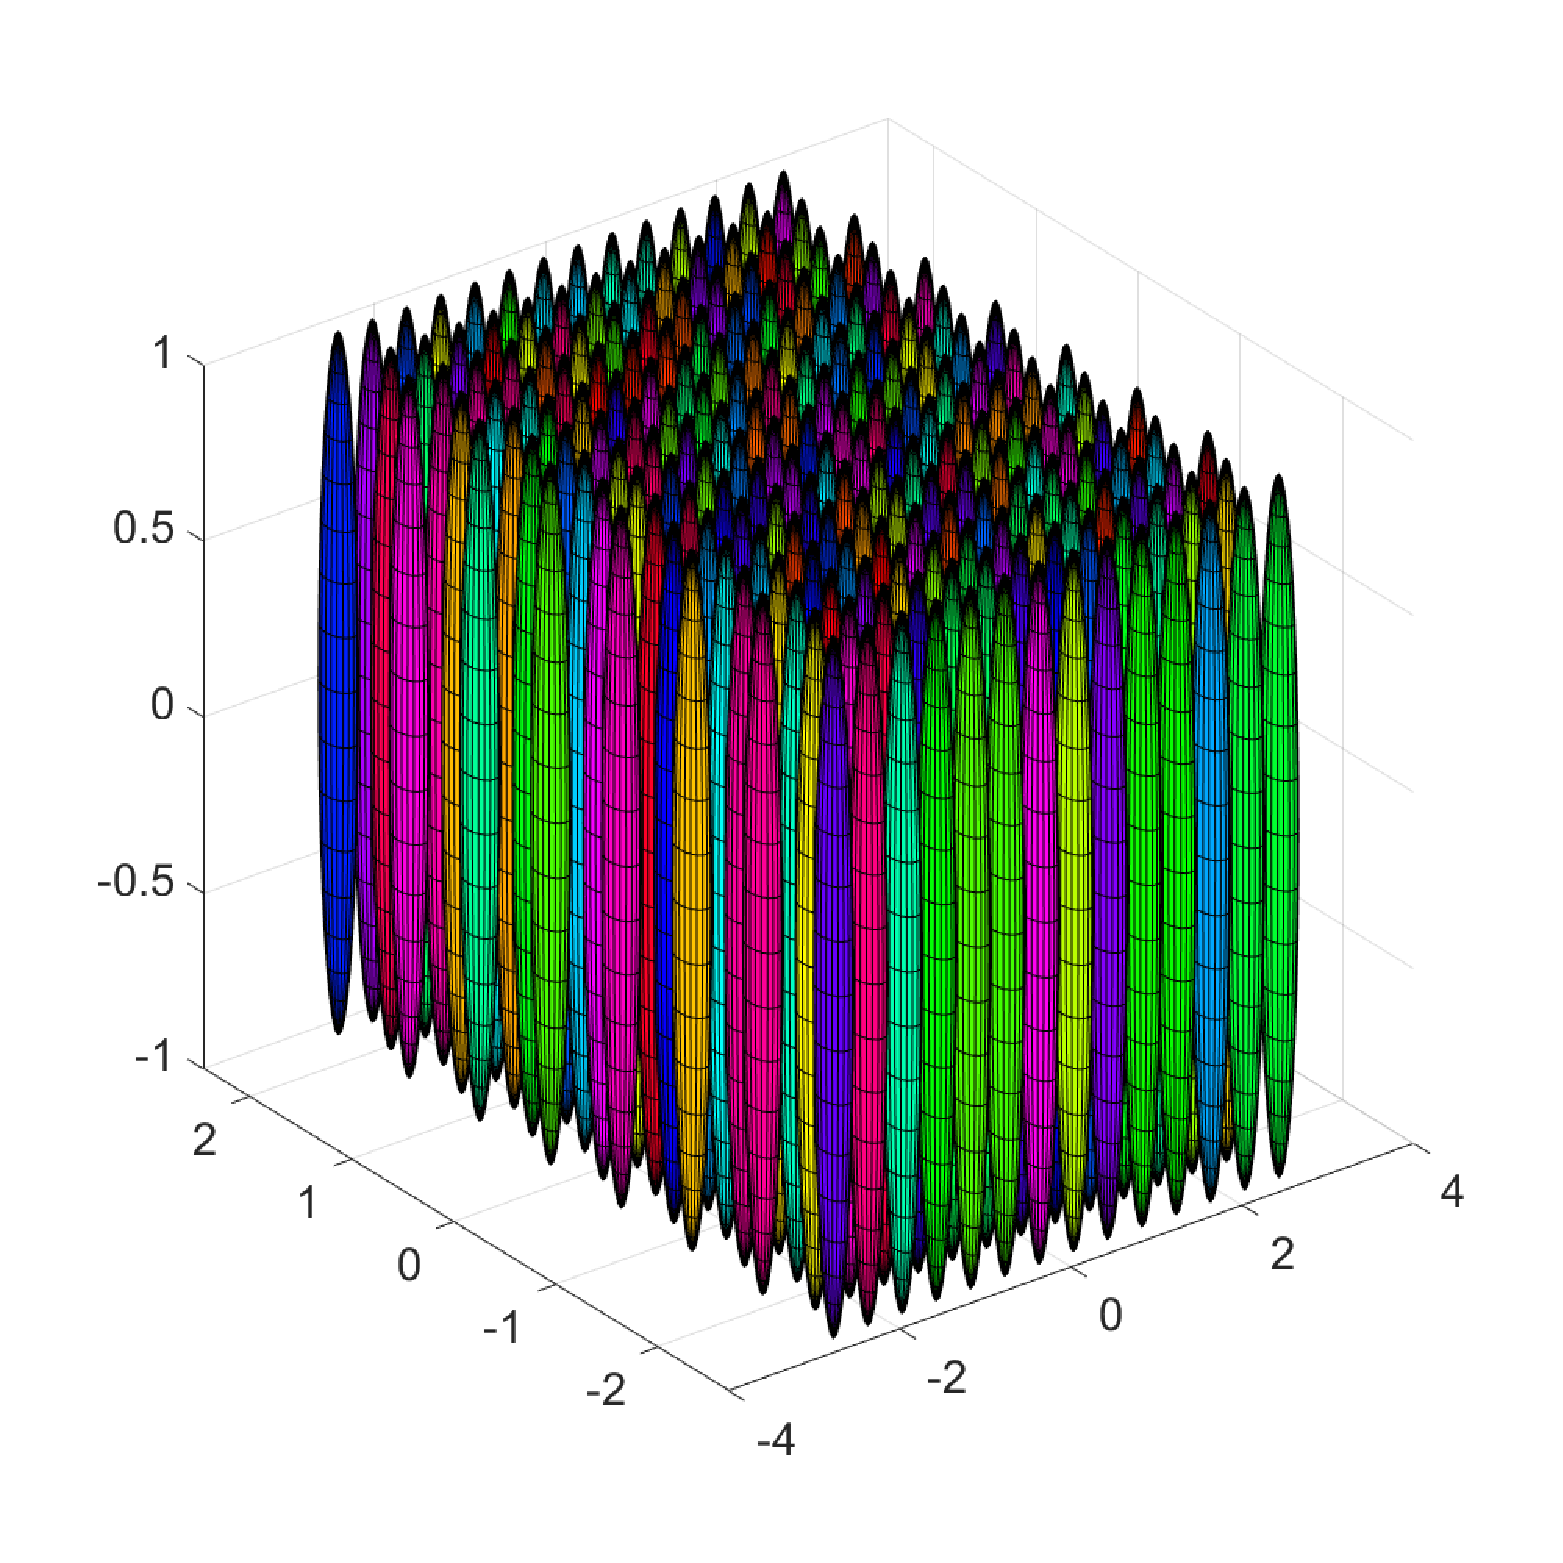
\includegraphics[width=\textwidth]{Images/Rods/SmallRods3d.pdf}
            \caption[]%
            {{\small 203 prolate spheroids in a three dimensional view}}    
            \label{fig:mean and std of net14}
        \end{subfigure}
        \begin{subfigure}[b]{0.475\textwidth}  
            \centering 
            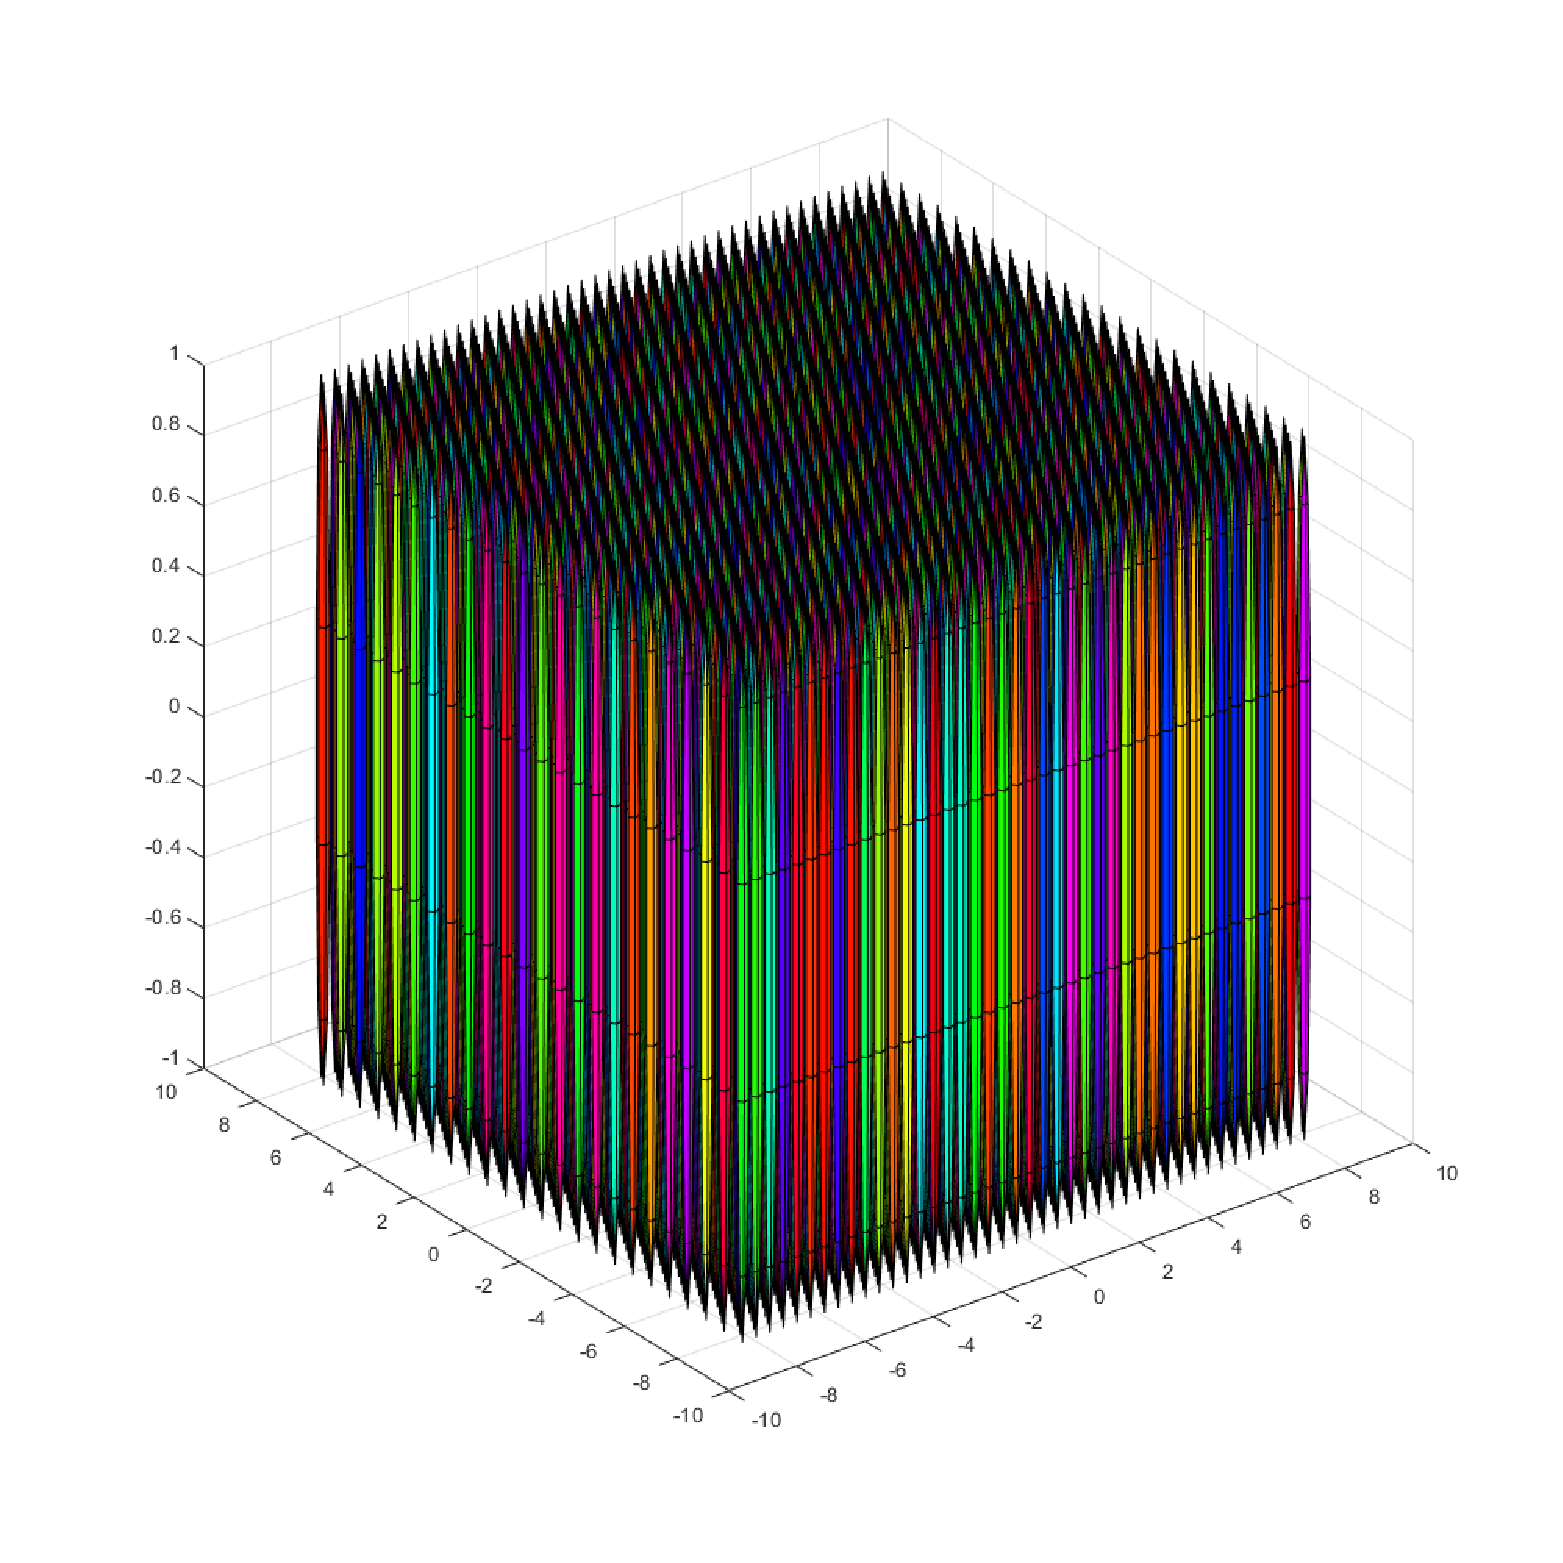
\includegraphics[width=\textwidth]{Images/Rods/LargeRods3d.pdf}
            \caption[]%
            {{\small 2016 prolate spheroids in a three dimensional view}}    
            \label{fig:mean and std of net24}
        \end{subfigure}
        \vskip\baselineskip
        \begin{subfigure}[b]{0.475\textwidth}   
            \centering 
            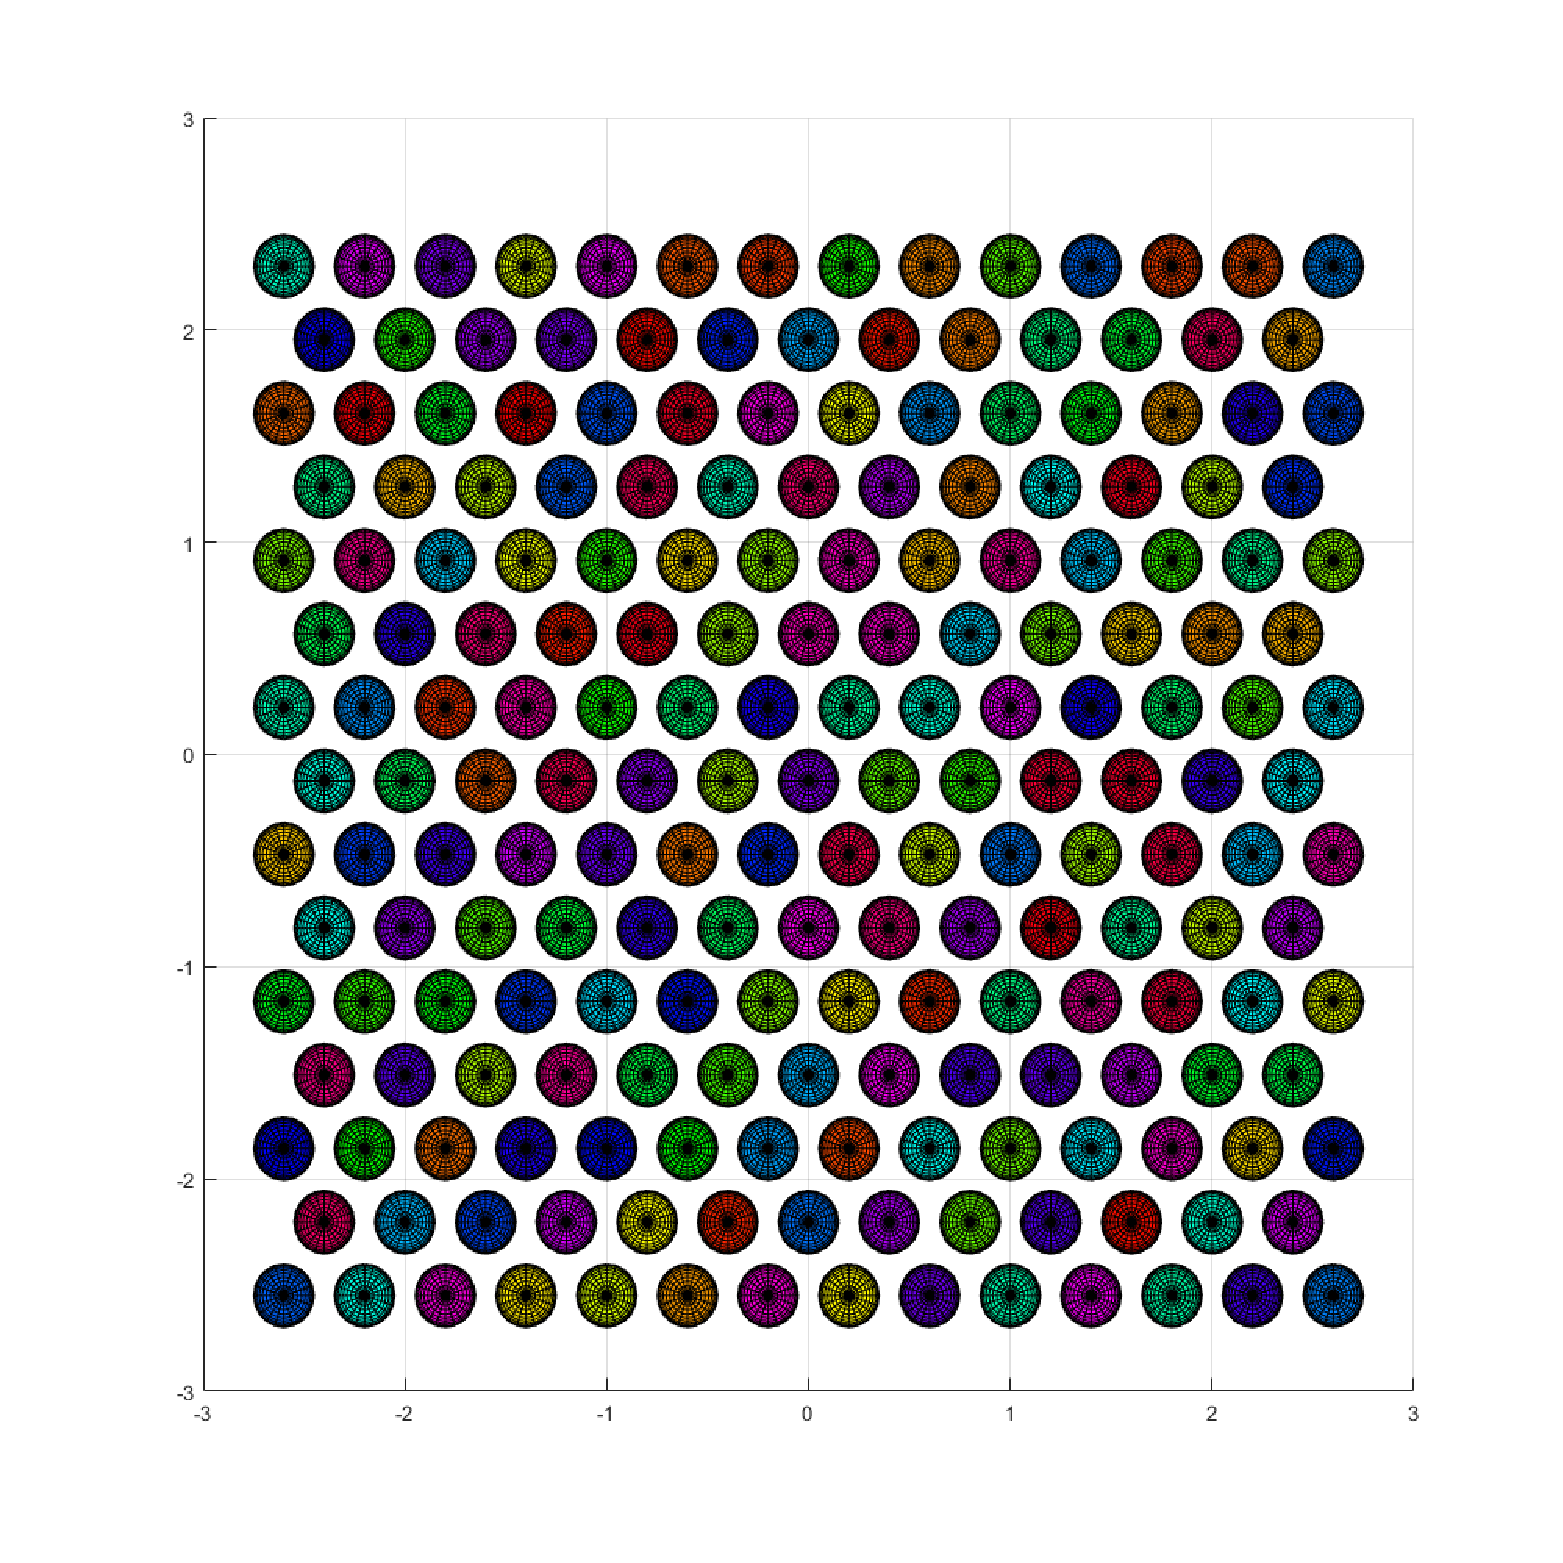
\includegraphics[width=\textwidth]{Images/Rods/SmallRodstop.pdf}
            \caption[]%
            {{\small 203 prolate spheroids from top down view}}    
            \label{fig:mean and std of net34}
        \end{subfigure}
        \hfill
        \begin{subfigure}[b]{0.475\textwidth}   
            \centering 
            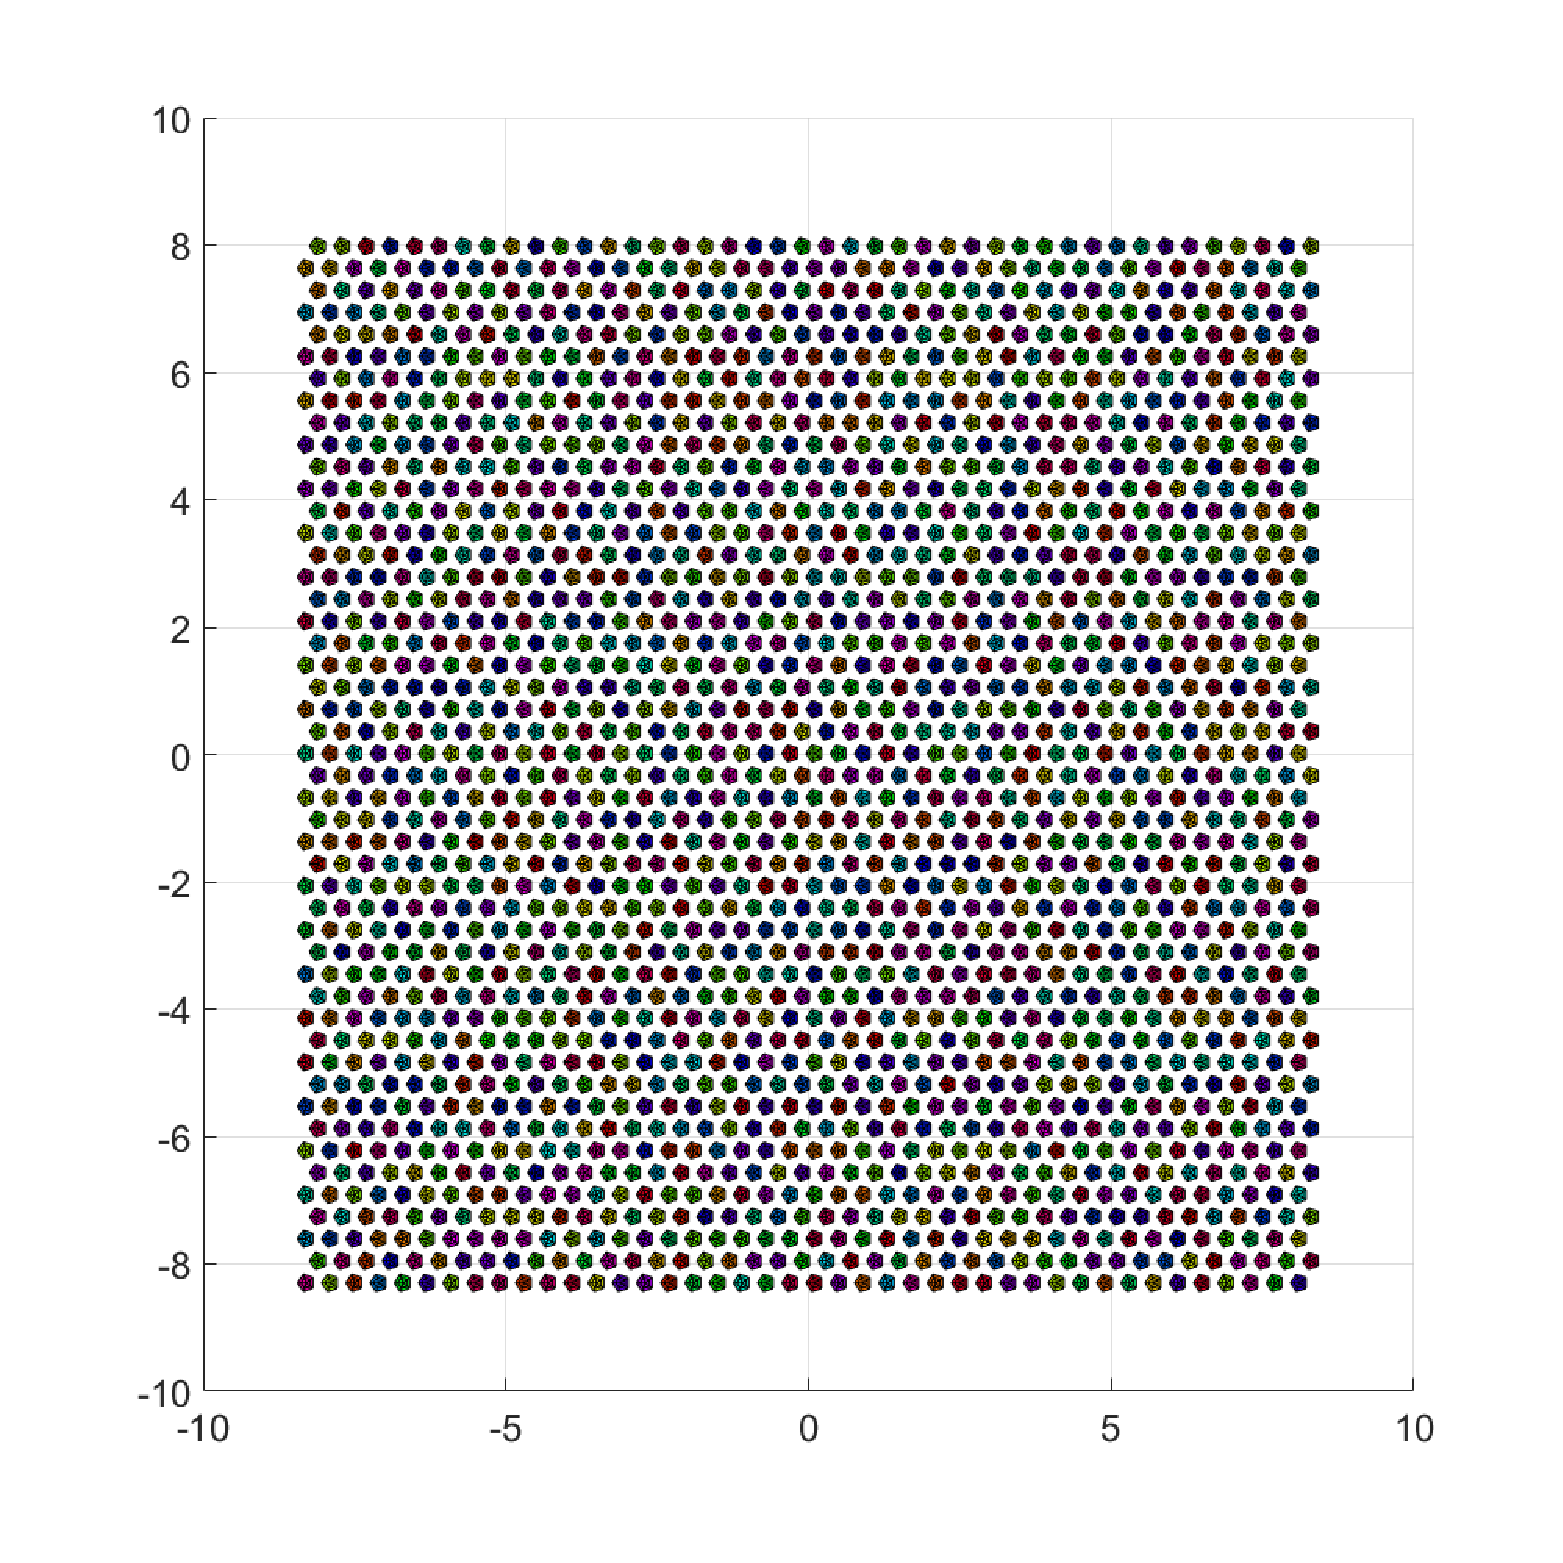
\includegraphics[width=\textwidth]{Images/Rods/LargeRodstop.pdf}
            \caption[]%
            {{\small 2016 prolate spheroids from top down view}}    
            \label{fig:mean and std of net44}
        \end{subfigure}
        \caption[Images of Rods in Shear flow]
        {\small Figure showing the configuration of prolate spheroids used in the two problems considered. Both problems are arranged on the same lattice spacing of $0.4$ units between each rod. A shear flow of 2 runs vertically from top to bottom such that the fluid velocity at the top has magnitude 1 at the top of the rods travelling in the positive x-direction (Left to right) and magnitude 1 at the bottom of the rods travailing in the negative x-direction (Right to left). This causes the rods to want to rotate about their central axis. } 
        \label{fig:mean and std of nets}
    \end{figure}


\subsection[Optimisations for the repeated evaluation of the KIFMM algorithm]{Optimisations for the repeated evaluation of the KIFMM algorithm%
\subsectionmark{Optimisations}}
\subsectionmark{Optimisations}

We will be solving this system through the use of GMRES (see \cref{appendix:GMRES}) as we are unable to form the full matrix with the KIFMM method. We can instead compute the swimming problem in blocks, we will compute the stokeslet matrix $A$ with the KIFMM method first before constructing the $B_i^U$, $B_i^\Omega$, $B_i^F$ and $B_i^M$ matrix blocks. For notational ease, we will group these into two matrices
\begin{equation*}
\arraycolsep=0.4pt\def\arraystretch{1}
B = \left( \begin{array}{ccc}
B_{1}^{F} & B_{2}^{F} & B_{3}^{F} \\
B_{1}^{M} & B_{2}^{M} & B_{3}^{M}
\end{array}\right) \text{ and }
B^\prime = \left(\begin{array}{cc}
B_{1}^{U} & B_{1}^{\Omega} \\
B_{2}^{U} & B_{2}^{\Omega} \\
B_{3}^{U} & B_{3}^{\Omega} \\
\end{array}\right).
\end{equation*} 
We construct both $B$ and $B^\prime$ outside of the GMRES method as they remain the same for all GMRES iterations. Optimisation within the KIFMM method could also be considered as all translations are again the same for all iterations. Profiling of the code shows that over 40\% of computation is due to the calculation of the stokeslet kernel which remain the same for each iteration. Precomputing all stokeslet matrices would provide the most optimal computation time however would require significant amounts of memory. Most implementations opt to only precompute the Multipole to Local (M2L) translations only as they form the largest proportion of the computation. A proposed option to reduce both the computation time and the memory requirements for the M2L translations is to use Fast Fourier Transforms (FFT) to compute the interactions \cite{Ying2004}. Considering an M2L translation of the potential $\{\bm{f}^{AU}\}$ of a node $A$ onto the downwards surface $\{\bm{q}^{BD}\}$ of a node $B$. Both the upwards and downwards equivalent potentials are defined to be a Cartesian grid with the same number of quadrature points, by padding the centre of each surface with gridpoints of $0$ density we can view the M2L translation as a 3D convolution that can be carried out efficiently by FFT. We would only need to compute a single FFT and IFFT (inverse fast Fourier transform) per node and element wide multiplication for each node in the $V$ or $W$ interaction lists. We have yet to implement this method, but look to explore this approach if further research requires it.

The S2L, L2L and M2M translations are often computed on each iteration due to the smaller number of translations or the overall size of the the matrices. In future implementations of the hybrid NEAREST KIFMM, pre-calculation of the S2L matrices could also be considered, along with SVD based compression, to reduce the memory cost of pre-calculation \cite{Drineas2006FAST,Cao2012ABEM} as these now form a larger part of the computation compared the standard method. Another promising optimisation to our current implementation is the use of dual tree traversal \cite{Yokota2013AnArchitectures:,Dehnen2002AAlgorithm,Carrier2006ASimulations,Wilson2021ATraversal} which does not require the need to compute interaction lists for each node.

In the hope to speed up the GMRES method without changing the underlying KIFMM method, we will explore how to reduce the required number of GMRES iterations required to converge to the required tolerance.

\subsubsection{Initial Guess}\label{sec:Guess}

An easily implemented attempt at reducing the total number of GMRES iterations is to provide an initial guess to the GMRES solver such that the initial relative residual error is already minimised and the number of iterations required to converge will be lower. As seen in \cref{appendix:ConNum} the condition number of the system decreases and the eigenvalues are more clustered with decreasing $\epsilon$, this means that in most cases the required number of GMRES iterations required for the system to converge will be smaller as seen in \cref{fig:InitalGuessEPS}.

\begin{figure}[ht]
    \centering
    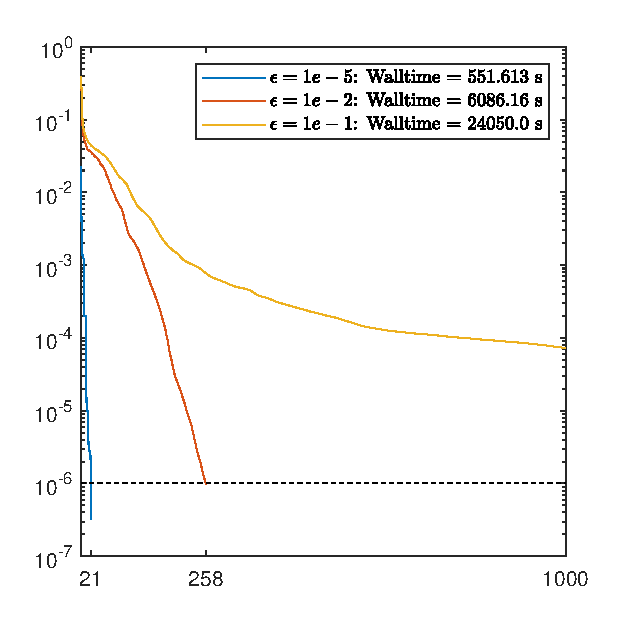
\includegraphics[width=0.5\textwidth]{Images/InitalGuessEPS.pdf}
    \caption{Convergence of the small rod problem with 3 different choices of epsilon. The $\epsilon = 10^{-1}$ problem did not converge in the given 1000 iterations.}
    \label{fig:InitalGuessEPS}
\end{figure}

Solving the problem for a smaller epsilon, however, does not give us an accurate initial guess for the actual problem with a larger epsilon, as the particle interactions are of a smaller magnitude. However, we note that the stokeslet matrix $A$ is dominated by the diagonal elements whose magnitude is proportional to $1/\epsilon$. If we consider two versions of the problem one with a smaller value of epsilon $\epsilon_1$ and stokeslet matrix $A_1$ and a target epsilon $\epsilon_2$ with a stokeslet matrix $A_2$ for which we would like to solve the problem. We first solve the initial problem with $\epsilon=\epsilon_1$, this should converge quickly in comparison to the second system and will return us a solution $\bm{F}_1$. The contribution to the first $3N_{F}$ terms are dominated by the diagonal elements of $\epsilon$ of order $1/\epsilon_1$ so by re-scaling the using a factor of $\epsilon_1/\epsilon_2$ we should have a better approximation to the solution. Very little has been published on the use of initial guesses with GMRES as often they provide little to no benefit to the overall computation. What is understood is the need for the residual from the initial guess $x_0$ to be lower than the residual of the right-hand side $b$ ($\lVert b-Ax_0 \rVert \leq \lVert r_o \rVert$). In order to achieve this, we use a trick outlined by Heged{\"u}s \cite{Saad1986GMRES:Systems,Strakos2005OnComputations} which minimises the residual using the method of least squares to obtain a scaling factor of 
\begin{equation*}
    \left\|r_{0}\right\|=\left\|b-A_2 \bm{F}_1 \zeta_{\min }\right\|=\min _{\zeta}\left\|b-A_2 \bm{F}_1 \zeta\right\|, \quad \zeta_{\min }=\frac{b^{T} A_2 \bm{F}_1}{\left\|A_2 \bm{F}_1\right\|^{2}}
    \label{eq:Hegedus}
\end{equation*}
where $\bm{F}_1$ is our initial guess from $A_2$ and our initial guess for the GMRES algorithm is $x_0 = \zeta_{\min} \bm{F}_1$. This initial guess gave some improvement in both cases as seen in \cref{tab:Preconditioning}.

\subsubsection{Rescaling Swimming Matrix} \label{sec:Rescale}
In the hope of cheaply reducing the condition of the matrix and more tightly clustering the eigenvalues of the swimming matrix, such that the GMRES algorithm converges in a smaller number of iterations \cite{CampbellGMRES}, we re-scale the $B$ matrix in \cref{eq:swimmingStructure} such that its maximum value is one. This should reduce the condition of the matrix and cluster the eigenvalues at the centre. We are able to do this due to the $0$ force and moment constraints that we have imposed upon the problem and as such we are able to re-scale our $B$ matrix without affecting the constraints. 
We do see a tighter clustering in the eigenvalues shown in \cref{appendix:ConNum} where the eigenvalues cluster closer to 1, however, the overall condition of the system increases.


\subsubsection{Preconditioning} \label{sec:Preconditioning}
A more optimal way in which we can optimise Krylov subspace methods is to use a preconditioner such that the matrix system we are trying to solve has a smaller condition number with more clustered eigenvalues. This reduces the effect of small perturbations made by the GMRES method. If we call the swimming matrix defined in \cref{eq:swimmingStructure} $M$, the vector of unknowns $\bm{x}$ and the right hand side $\bm{b}$ then we can refer to the system as $Mx=b$. The matrix $M$ is significantly less well-conditioned (see \cref{appendix:ConNum}) than the stokeslet matrix $A$ and as such requires a significant number of iterations to solve.

Our preconditioner is based on work by Rostami and Olson \cite{Rostami2019FastBiofluids} and is inspired by the so-called “least-squares commutator” preconditioner \cite{Elman2005FiniteDynamics}. As described above we group the augmenting matrices into two larger matrices denoted $B$ and $B^\prime$. This means our swimming matrix can be written as 
\begin{equation*}
\begin{aligned}
\def\arraystretch{0.8}
    M = \left(\begin{array}{cc}
        A & B^\prime \\
        B & 0_{6N_{sw}\times6N_{sw}} 
    \end{array}\right) &= 
    \left(\begin{array}{cc}
        \mathds{1}_{3N_F \times 3N_F} & O_{3N_F\times6N_{sw}} \\
        BA^{-1} & \mathds{1}_{6N_{sw} \times 6N_{sw}}
    \end{array}\right)
    \left(\begin{array}{cc}
        A & B^\prime \\
        O_{6N_{sw}\times3N_F} & -BA^{-1}B^\prime
    \end{array}\right) \\
    &= LU.
\end{aligned}
\end{equation*}

This means $MU^{-1}$ has eigenvalues of 1 and as such GMRES should converge in one iteration \cite{Rostami2019FastBiofluids} if $U^{-1}$ is used as a right preconditioner to solve the system $MU^{-1}y = b$ where $x = U^{-1}y$. However due to the need to solve $BA^{-1}B^\prime$ this becomes infeasible, particularly when we do not construct $A$ explicitly.  Instead, we will attempt to cheaply approximate $U^{-1}$. We will denote the preconditioner matrix 
\begin{equation}
\def\arraystretch{0.8}
    P_M = \left(\begin{array}{cc}
        P_A & B^\prime \\
        O_{6N_{sw}\times3N_F} & P_S
    \end{array}\right)
    \label{eq:Precon}
\end{equation}
where $P_A$ is a preconditioner for the matrix $A$ and $P_S$ is a preconditioner for $-BA^{-1}B^\prime$. The Schur complement \cite{Zhang2005TheApplications,Lu2002InversesMatrices} allows us to compute the inverse of a $2 \times 2$ block matrix as 
\begin{equation*}
\def\arraystretch{0.8}
    \left(\begin{array}{cc}
        A & B \\
        C & D
    \end{array}\right)^{-1} = \left(\begin{array}{cc}
A^{-1}+A^{-1} B\left(D-C A^{-1} B\right)^{-1} C A^{-1} & -A^{-1} B\left(D-C A^{-1} B\right)^{-1} \\
-\left(D-C A^{-1} B\right)^{-1} C A^{-1} & \left(D-C A^{-1} B\right)^{-1}
\end{array}\right) 
\end{equation*}
if $A$ is invertible. This gives that the inverse of our preconditioner matrix \cref{eq:Precon} is
\begin{equation*}
\def\arraystretch{0.8}
        P_M^{-1} = \left(\begin{array}{cc}
        P_A^{-1} & -P_A^{-1} B^T P_S^{-1} \\
        O_{6N_{sw}\times3N_F} & P_S^{-1}
    \end{array}\right)
\end{equation*}
We, therefore, need to solve two systems of equations involving $P_A$ and one linear system involving $P_S$. As we stated above, solving a linear system involving $P_S$ is too computationally challenging to form and solve, so we must look for an approximation to this solution. Inspired by the method of least squares we look for a solution $C$ which minimises the residual of $\lVert AB^T - B^\prime C \rVert \;\forall\; C \in \mathbb{R}^{6N_{sw}\times6N_{sw}}$. This solution is found by taking the square of the residual to obtain $(AB^T - B^\prime C)^T(AB^T - B^\prime C) = (AB^T)^T(AB^T)-(AB^T)^TB^\prime C-C^T(B^\prime)^TA^T + C^T(B^\prime)^TB^\prime C$. Taking the derivative of this with respect to $C$ equal to $0$ will minimise the residual squared. This yields $-2(B^\prime)^TAB^T + 2(B^\prime)^TB^\prime C=0$ so $C = ((B^\prime)^TB^\prime)^{-1}(B^\prime)^TAB^T$. Computing the inverse of $C$ we get that $C^{-1} = ((B^\prime)^TAB^T)^{-1}((B^\prime)^TB^\prime)$. As we have minimised the residual, we can say that $AB^T \approx B^\prime C \implies B^T C^{-1} = A^{-1}B^\prime$. Substituting both of these into our equation for our preconditioner $P_S$ gives us that, 
\begin{equation}
\begin{aligned}
    P_S = - B A^{-1}B^\prime &= -B B^{T} C^{-1} \\
    & = -(B B^{T})((B^\prime)^TAB^T)^{-1}((B^\prime)^TB^\prime) \\
    \implies P_S^{-1} &= -((B^\prime)^TB^\prime)^{-1}((B^\prime)^TAB^T)(B B^{T})^{-1}
\end{aligned}
\label{eq:PreconS}
\end{equation}

The computation of $P_S^{-1}$ now only involves solving the linear systems $(B^\prime)^TB^\prime$ and $B B^{T}$, however, these are cheap and easy to solve as both matrices are mainly sparse with dominant diagonal elements due to their construction. We still need to compute the solution to $P_A^{-1}$. We will consider solving this via a block diagonal form of the KIFMM where we only consider the interactions between nodes. 
The block diagonal preconditioner captures most of the dominant interactions between particles and provides a relatively accurate estimation of the solution to $A^{-1}$ and is significantly quicker to run. It also reduces the system to a set of simpler problems, one for each node. These are quicker and easier for GMRES to solve and, as such, the method can converge rapidly for these systems. This principle could be extended to include all nodes in the $U$ interaction list, this provides better results for a single pass, however, due to the off-diagonal elements now being included, the problem is less well-conditioned with longer interaction times so we will only consider the purely block-diagonal preconditioner. Block diagonal preconditions have been used to solve problems in systems using the Rotne-Prager-Yamakawa (RPY) tensor \cite{UsabiagaHYDRODYNAMICSAPPROACH}, stokeslet\cite{Nazockdast2017AMechanics} and more general elliptical PDEs \cite{Ibeid2018FastEquations}. 

Following on from using the diagonal preconditioner for $P_A^{-1}$ we will also consider a cheaper approximation to full matrix multiplication of $A$ in the computation of $P_S^{-1}$. Following on from the results shown in \cref{fig:QuadPoints} we note a  cheaper but less accurate computation can be achieved by using fewer quadrature points for the equivalent surfaces, in this way, 60 quadrature points were chosen as it provided a good balance between the accuracy of the method and provides a noticeable speed increase compared to the full method with 152 quadrature points. 

\subsection{Results}



The results of all 3 optimisations can be seen in \cref{tab:Preconditioning} along with data for the non preconditioned system. All methods had a fixed stopping criterion of $\lVert Mx-b \rVert_2/\lVert b \rVert_2 \leq 10^{-6}$ as is the default in MATLAB's GMRES method. The 2016 swimmer model proved challenging to solve with over 150 more GMRES iterations needed to converge to the same tolerance when no preconditioner was used. Both methods were aided by the use of an initial guess with the computation time being reduced by nearly 10\% as the initial iterations are replaced by quicker iterations using a smaller $\epsilon$ value. The attempt at re-scaling the lower augmented matrix was proven to increase the overall computation time, where the tighter clustered eigenvalues did not allow the method to converge any quicker. More work could be done in order to find a correct scaling factor to keep the tightly clustered eigenvalues and reduce the overall condition of the matrix. 

\begin{table}
\begin{singlespace}
\centering
\setlength{\tabcolsep}{6pt}
\renewcommand{\arraystretch}{1.4}
\caption{Comparison of preconditioners in the case of Rods in Shear Flow. All methods converged to a relative residual error smaller than $10^{-6}$}
\small
\begin{tabular}{p{2cm} p{1cm} p{2cm} p{1.5cm} p{0.1cm} p{1cm} p{2cm} p{1.5cm}}
\multirow{2}{*}{\parbox{1.8cm}{number of swimmers}} & \multicolumn{3}{l}{No precondtioner} & & \multicolumn{3}{l}{Initial Guess} \\ \cline{2-4} \cline{6-8}
  & \# of iters & \# of MVPs ($M$) & walltime (sec.) & & \# of iters & \# of MVPs ($M_{\epsilon_1}/M_{\epsilon_2}$) & walltime (sec.) \\ \hline
  203 & 250 & 250 & 8599 & &  268 & 20/248 & 7763\\
  2016 & 409 & 409 & 23645 & & 358 & 12/346 & 20977\\ \hline
  \multirow{2}{*}{\parbox{1.8cm}{number of swimmers}} & \multicolumn{3}{l}{Rescaling} & &\multicolumn{3}{l}{Least-squares commutator} \\ \cline{2-4} \cline{6-8}
  & \# of iters & \# of MVPs ($M$) & walltime (sec.) & & \# of iters & \# of MVPs ($M/P_A^{-1}/A_S$) & walltime (sec.) \\ \hline
  203 & 297 & 297 & 9357 & & 71 & 62/124/63 & 3739 \\
  2016 & 523 & 523 & 34036 & & 47 & 47/96/48 & 4165 
\end{tabular}
\label{tab:Preconditioning}
\end{singlespace}
\end{table}

As expected, preconditioning of the system proved most effective in reducing the overall computation time, particularly with the 2016 swimmer case where the computation time drops by 80\%. The 203 swimmer case does not see such a significant drop with a decrease in computation time of 50\%, possibly due to the larger contribution that the stokeslet matrix $A$ has on the computation. We would expect to see that, for systems with more swimmers and the same number of quadrature points, the number of GMRES iterations needed to converge would stay approximately the same, and as such, larger systems could be tackled. Combinations of these methods may prove useful in reducing the calculation further, such as initial guesses for preconditioned systems, however, due to the rapid decrease in the residual from the preconditioned system, it is doubtful that it will provide any noticeable gain and the need to use the Heged{\"u}s `trick' involves another full matrix product.

\begin{table}
\begin{singlespace}
\centering
\setlength{\tabcolsep}{6pt}
\renewcommand{\arraystretch}{1.4}
\caption[The use of hybrid KIFMM NEAREST method to solve the 2016 rod case.]{The use of hybrid KIFMM NEAREST method to solve the 2016 rod case. Both preconditioned and not preconditioned methods converged to a relative residual error smaller than $10^{-6}$ of the Joint case. Neither system converged in the maximum 1000 iterations for the Disjoint case.}
\small
\begin{tabular}{p{2cm} p{0.75cm} p{2cm} p{1.0cm} p{0.1cm} p{0.75cm} p{2.5cm} p{1.5cm}}
\multirow{2}{*}{\parbox{1.8cm}{NEAREST Spacing}} & \multicolumn{3}{l}{No precondtioner} & & \multicolumn{3}{l}{Least-squares commutator} \\ \cline{2-4} \cline{6-8}
  & \# of iters & \# of MVPs ($M$) & walltime (sec.) & & \# of iters & \# of MVPs ($M/P_A^{-1}/A_S$) & walltime (sec.) \\ \hline
  Joint & 201 & 201 & 2898 & &  47 & 47/96/48 & 1394\\
  Disjoint & 1000 & 1000 & 10436 & & 1000 & 1000/2002/1001 & 19734
\end{tabular}
\label{tab:PreconditioningNear}
\end{singlespace}
\end{table}

In order to evaluate the use of the hybrid KIFMM NEAREST method we solved the swimming problem for the case of 2016 in a shear flow. In order to compare between non NEAREST and NEAREST computations we discretise each spheroid with 42 fine quadrature points matching the discretisation in the non-nearest case and introduce a coarse discretisation with spacing 2 times larger such that the surface is discretised by 12 force quadrature points.  This gives a total of 72576 SDOF for each system with 84672 and 108864 fine quadrature points for the joint and disjoint cases respectively. Although results will differ slightly based on \cref{fig:NEARESTCOMPFMM,fig:NEARESTCOMP} and data collected by Smith \cite{Smith2018AEquation} show that the overall difference will be small. Figure \ref{tab:PreconditioningNear} shows that we see a large increase in performance for the joint case with a 2.7 times speed increase in the computation for the preconditioned system. The overall increase in speed obtained by using a preconditioner is only 2 times, compared to the 5 times speed increase found in the non NEAREST computations. Results for the disjoint case are less promising with neither simulation converging in 1000 iterations. The convergence rate of both systems appears to stagnate early with the pre-conditioned system failing to converge to a residual error of $4\times 10^{-2}$. This is due to the choice of the block-diagonal preconditioner which does not represent the system as closely as it does for other discretisations. 

\begin{figure}
    \centering
    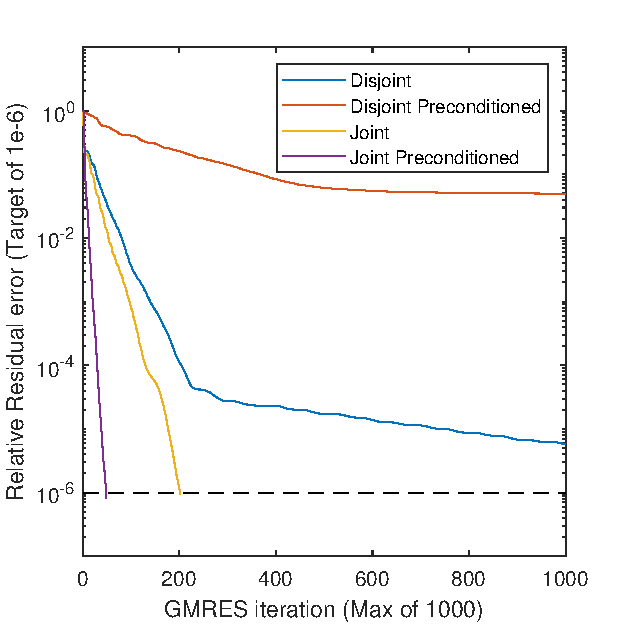
\includegraphics[width=0.5\textwidth]{Images/Rods/NearestPrecon.pdf}
    \caption{Convergence rate of NEAREST discretisation when used to solve the rods in a shear flow problem.}
    \label{fig:NearestConverge}
\end{figure}

\subsection{Squirmers}
The slip velocity spherical squirmer is used widely in models of propulsion in Stokes flow \cite{Smith2021TheSelf-Propulsion,Lauga2020TheModel,Pedley2016SquirmersSwimming}. The squirmer model allows for the representation of swimming motion generated by many beating cilia without the need to simulate each cilium individually. By scaling the coordinate system such that the radius of the spherical squirmer is 1, we denote an angle relative to the north pole as $\theta$ which lies between $0\leq\theta\leq\pi$. We also define $\bm{t}(\theta)$ to be the tangent to the sphere pointing towards the south pole. Then the velocity in the body frame of the the squirmer is $\bm{u}(\theta) = \sin(\theta)\bm{t}(\theta)$ as seen in \cref{fig:Squiremer3D}. We also plot the streamlines around the squirmers in \cref{fig:Squiremer3DFlow}, where the force at each force discretisation point on the squirmer is solved through the resistance problem. In order to refine the accuracy of the flow field, the hybrid NEAREST method was used with 3756 SDOF based on 1252 force quadrature points and 20058 fine quadrature points. The force field was then evaluated on a Cartesian grid in the domain $[-2\; 2] \times [-2\; 2] \times [-2\; 2]$ with a total of 125000 evaluation points. 

\begin{figure}
\begin{subfigure}[b]{0.4\textwidth}
    \centering
    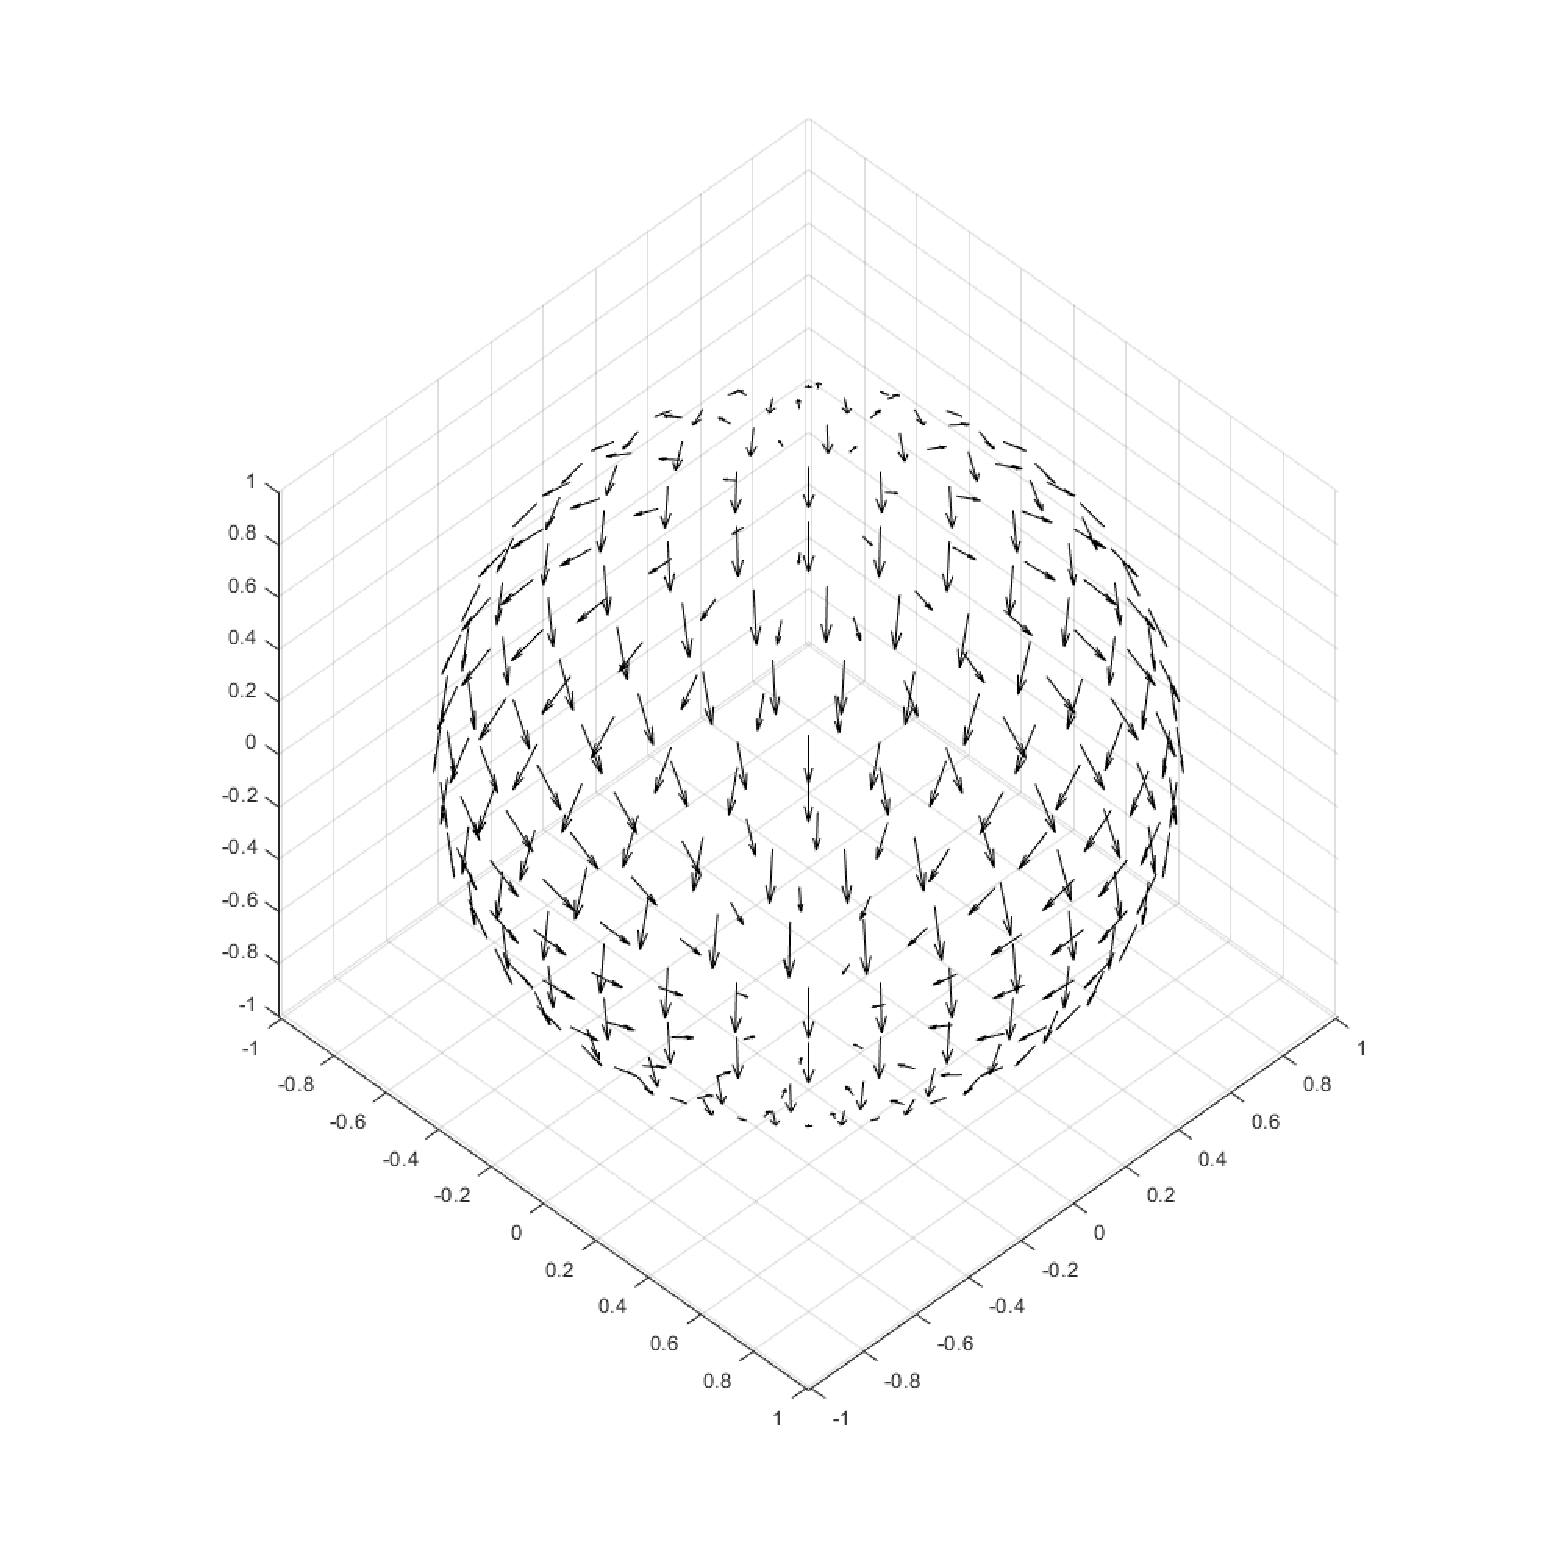
\includegraphics[width=\textwidth]{Images/squirmers/Squiremer3D.pdf}
    \caption[]{\label{fig:Squiremer3D}}
\end{subfigure}
\hfill
\begin{subfigure}[b]{0.4\textwidth}
    \centering
    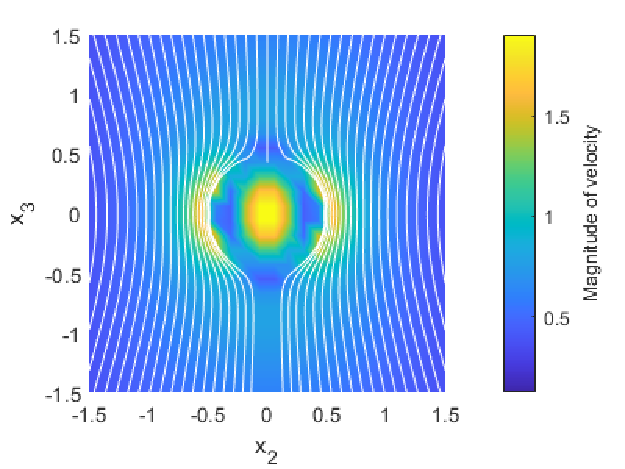
\includegraphics[width=\textwidth]{Images/squirmers/StreamLinesSingle.pdf}
    \caption[]{\label{fig:Squiremer3DFlow}}
\end{subfigure}
\caption[Velocity and Streamlines flow around a single squirmer.]{(i) Graph showing the magnitude of the velocity on the surface of a single squirmer. (ii) The computed velocity profile with streamlines in the $(x_2,x_3)$ plane}
\end{figure}

The interactions of multiple squirmers are considered in \cref{fig:Squiremer3DFlowPair} where we first solve a swimming problem, each swimmer is discretised with 1252 force quadrature points and 20058 fine quadrature points, totalling 7524 SDOF for each swimming problem. Noting that $\bm{b}^{(3)} = \bm{b}^{(1)} \times \bm{b}^{(2)}$ we only need to return the changes in the first two basis vectors, at each time step we return 
\begin{equation*}
    {\dot{\bm{x}}}_{0}=\bm{U}\left(\bm{x}_{0}, \bm{b}^{(1)}, \bm{b}^{(2)}, t\right), \quad \dot{\bm{b}}^{(j)}=\bm{\Omega}\left(\bm{x}_{0}, \bm{b}^{(1)}, \bm{b}^{(2)}, t\right) \times \bm{b}^{(j)}, \quad j=1,2
\end{equation*}
in the form
\begin{equation*}
\arraycolsep=0.4pt\def\arraystretch{1}
\dot{Y} = \begin{bmatrix}
    {\dot{\bm{x}}_{0 j}} \\
    {\dot{\bm{b}}^{(1)}}_j \\
    {\dot{\bm{b}}^{(2)}}_j
\end{bmatrix} \quad \text{ for } j=1,..,N_{sw}
\end{equation*}
The problem is then formulated by a set of $9 \times N_{sw}$ differential equations which can be solved using Matlab's \textit{ode45} solver. The resistance problem is then solved for the required time steps and the velocity is evaluated on a cartesian grid in the domain $[-3\; 3] \times [-3\; 3] \times [-3\; 3]$ with a total of 125000 evaluation points. Figure \ref{fig:Squiremer3DFlowPair} shows the flow field at select time steps during the simulation. A regularisation parameter of $10^{-2}$ was chosen such the condition of the resistance problem was relatively low and a fine quadrature spacing of a quarter of the force spacing was used as recommended by Smith and Gallagher \cite{Gallagher2020}.  

\begin{figure}
\centering
\begin{subfigure}[b]{0.328\textwidth}
    \centering
    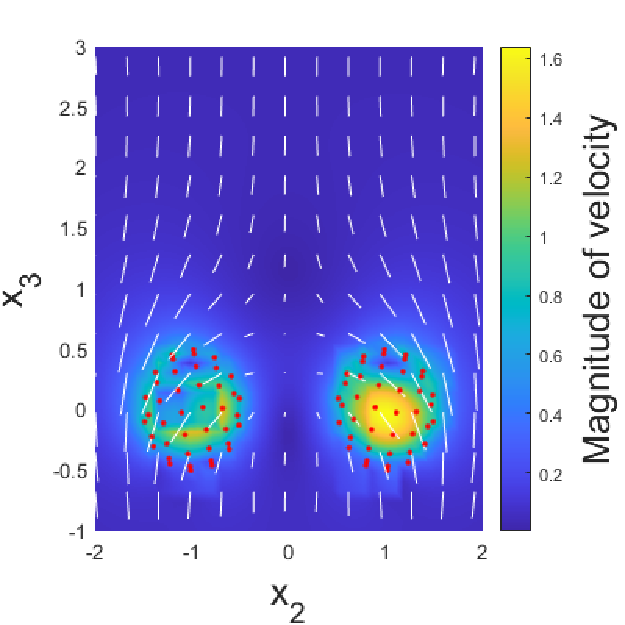
\includegraphics[width=\textwidth]{Images/squirmers/Pair-1.pdf}
    \caption[]{\label{fig:PairA}}
\end{subfigure}
\begin{subfigure}[b]{0.328\textwidth}
    \centering
    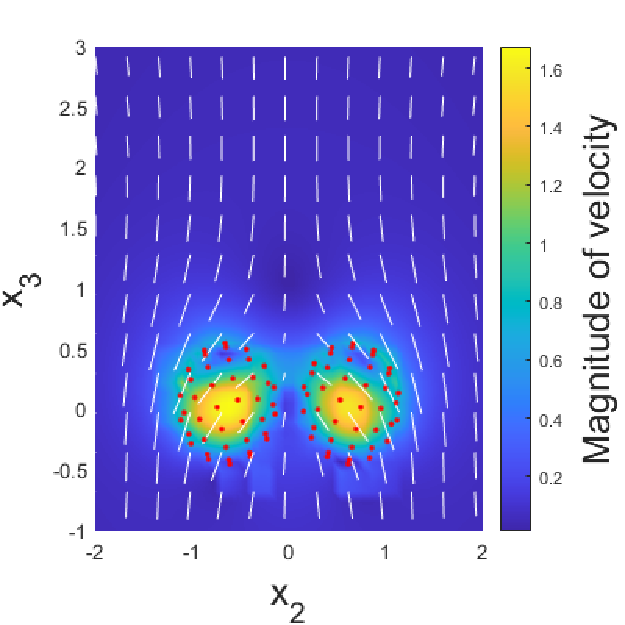
\includegraphics[width=\textwidth]{Images/squirmers/Pair-2.pdf}
    \caption[]{\label{fig:PairB}}
\end{subfigure}
\begin{subfigure}[b]{0.328\textwidth}
    \centering
    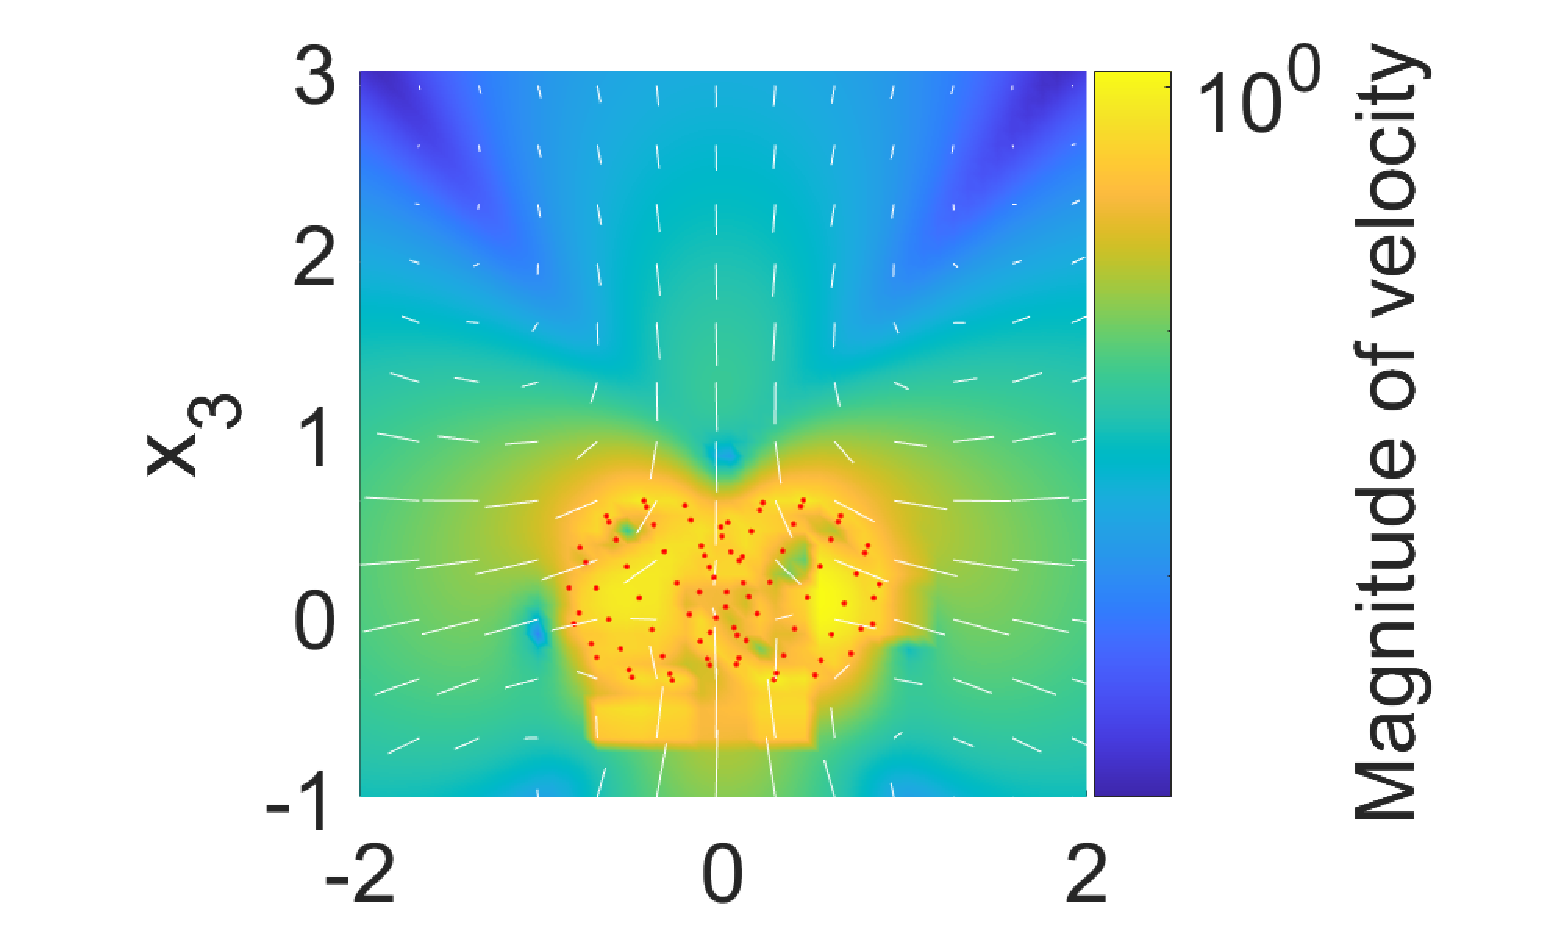
\includegraphics[width=\textwidth]{Images/squirmers/Pair-3.pdf}
    \caption[]{\label{fig:PairC}}
\end{subfigure}
\begin{subfigure}[b]{0.328\textwidth}
    \centering
    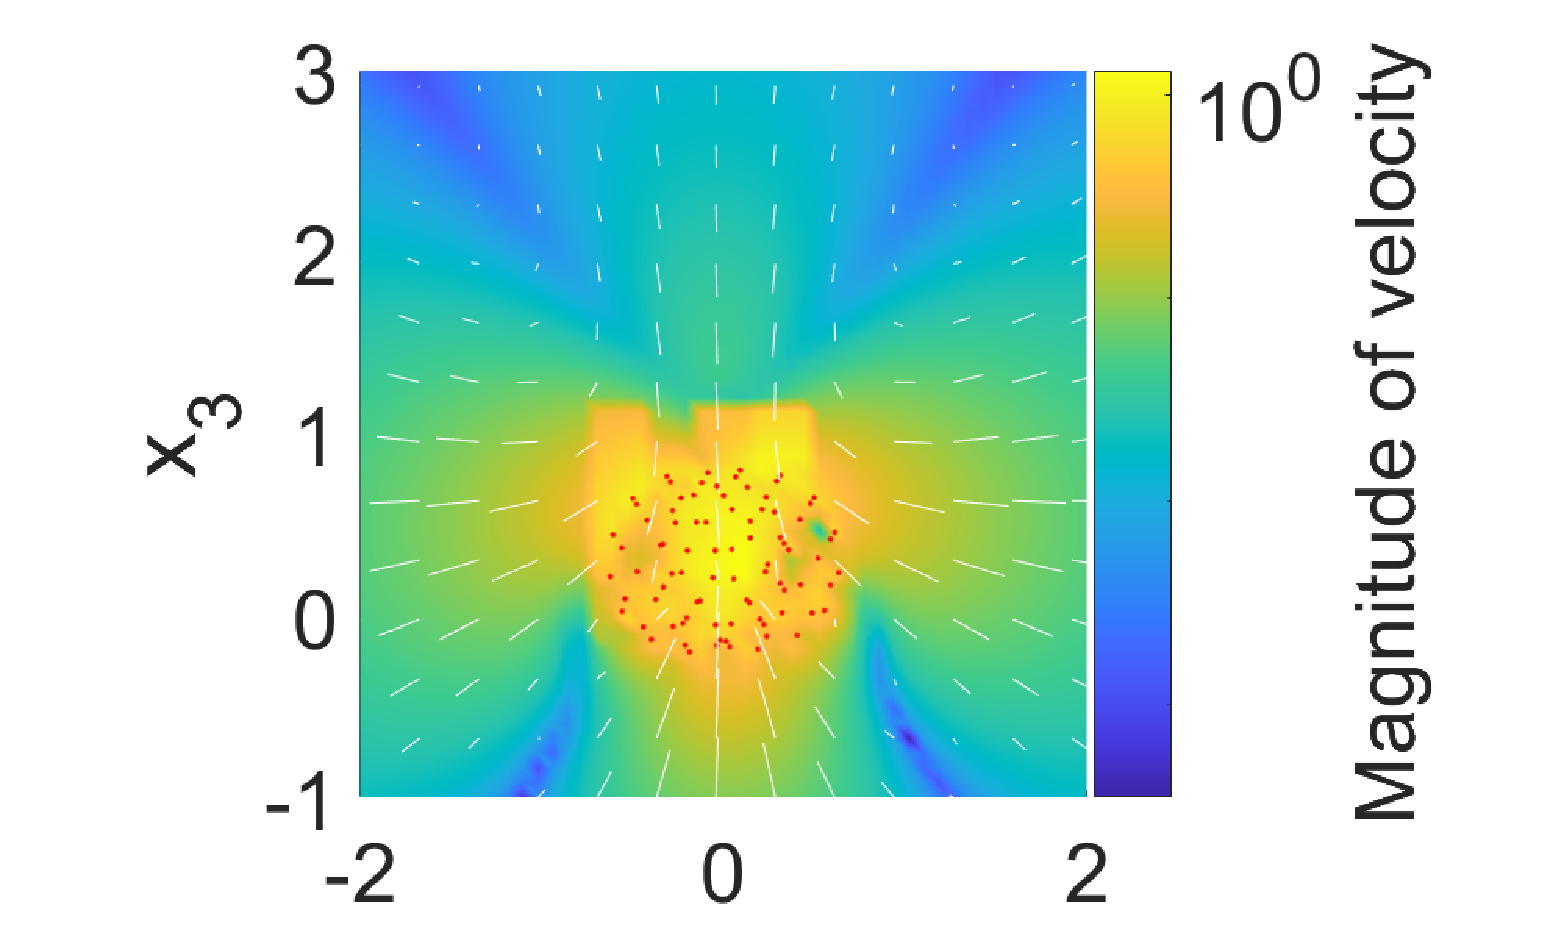
\includegraphics[width=\textwidth]{Images/squirmers/Pair-4.pdf}
    \caption[]{\label{fig:PairD}}
\end{subfigure}
\begin{subfigure}[b]{0.328\textwidth}
    \centering
    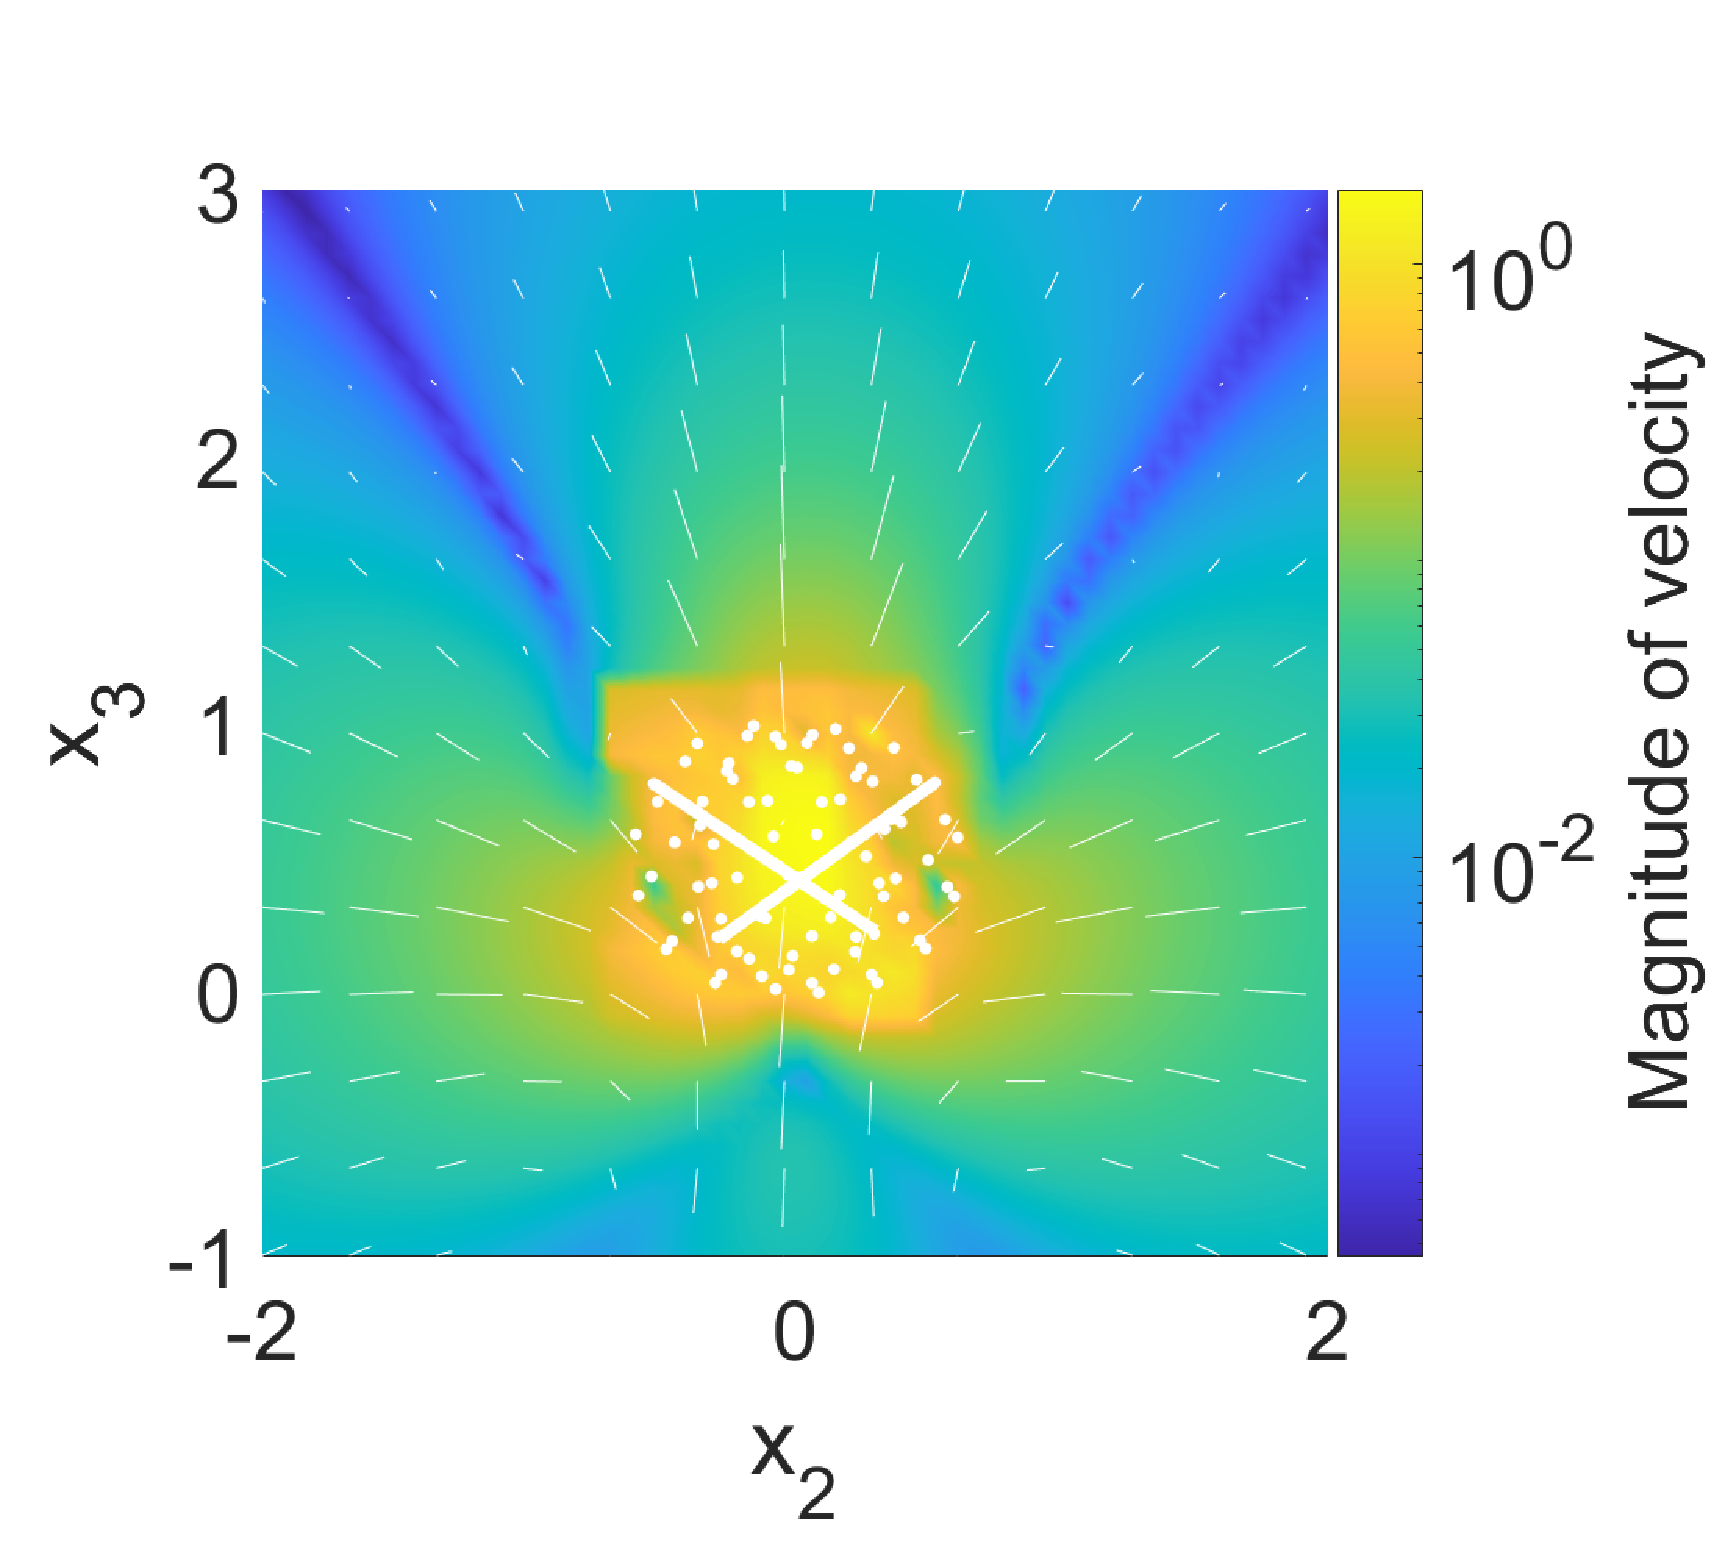
\includegraphics[width=\textwidth]{Images/squirmers/Pair-5.pdf}
    \caption[]{\label{fig:PairE}}
\end{subfigure}
\begin{subfigure}[b]{0.328\textwidth}
    \centering
    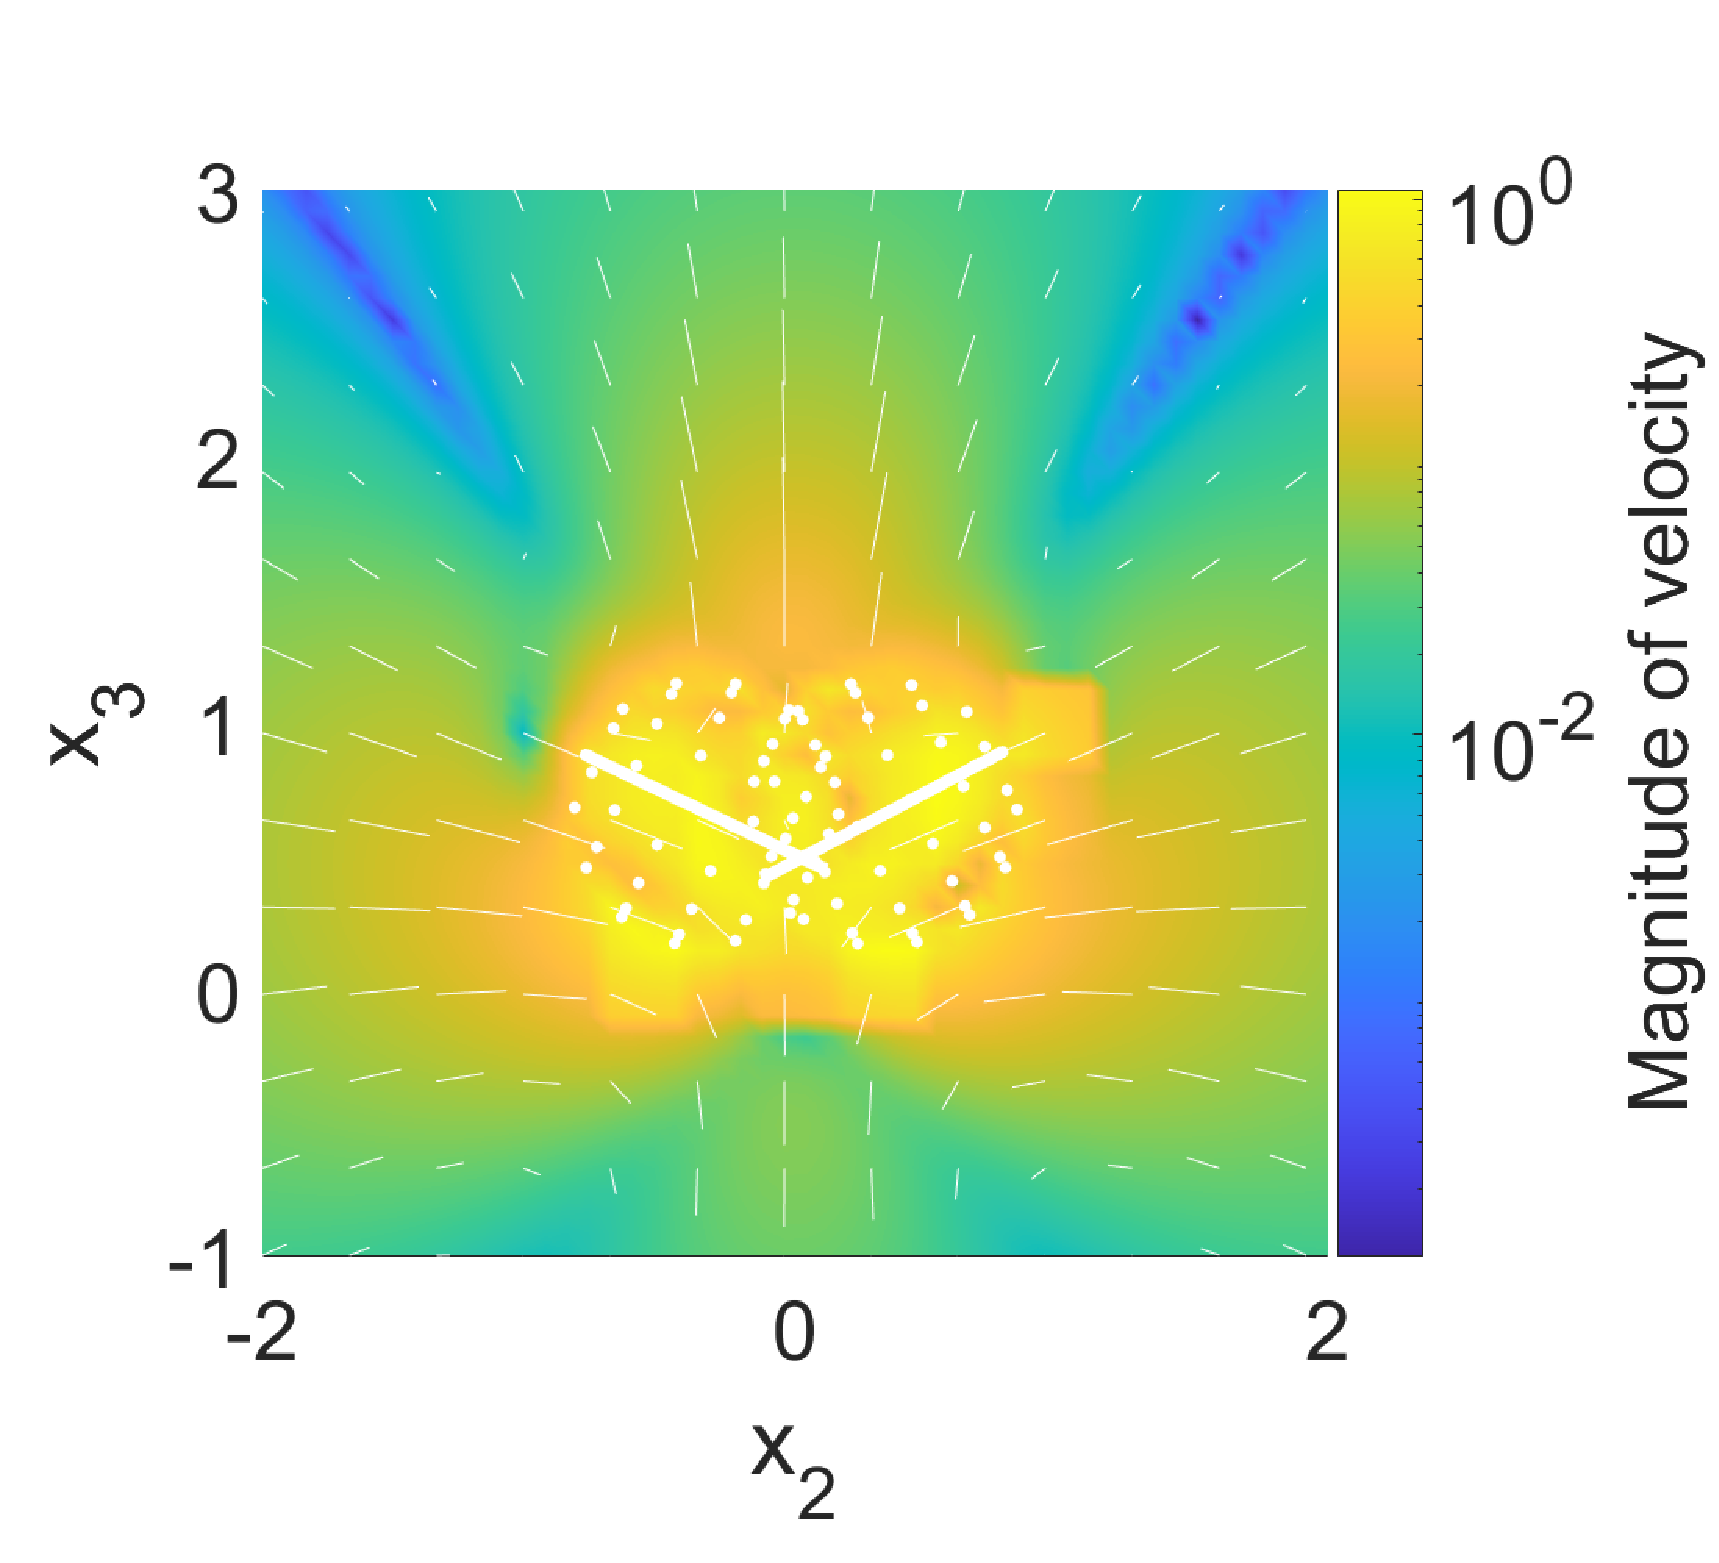
\includegraphics[width=\textwidth]{Images/squirmers/Pair-6.pdf}
    \caption[]{\label{fig:PairF}}
\end{subfigure}
\begin{subfigure}[b]{0.328\textwidth}
    \centering
    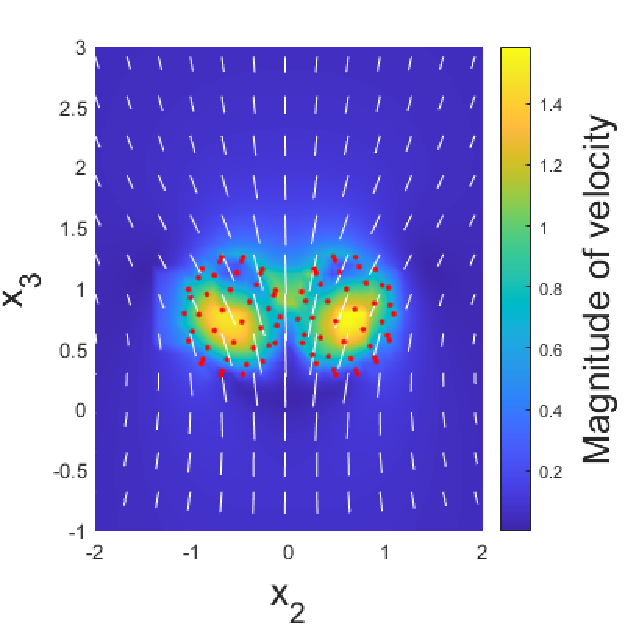
\includegraphics[width=\textwidth]{Images/squirmers/Pair-7.pdf}
    \caption[]{\label{fig:PairG}}
\end{subfigure}
\begin{subfigure}[b]{0.328\textwidth}
    \centering
    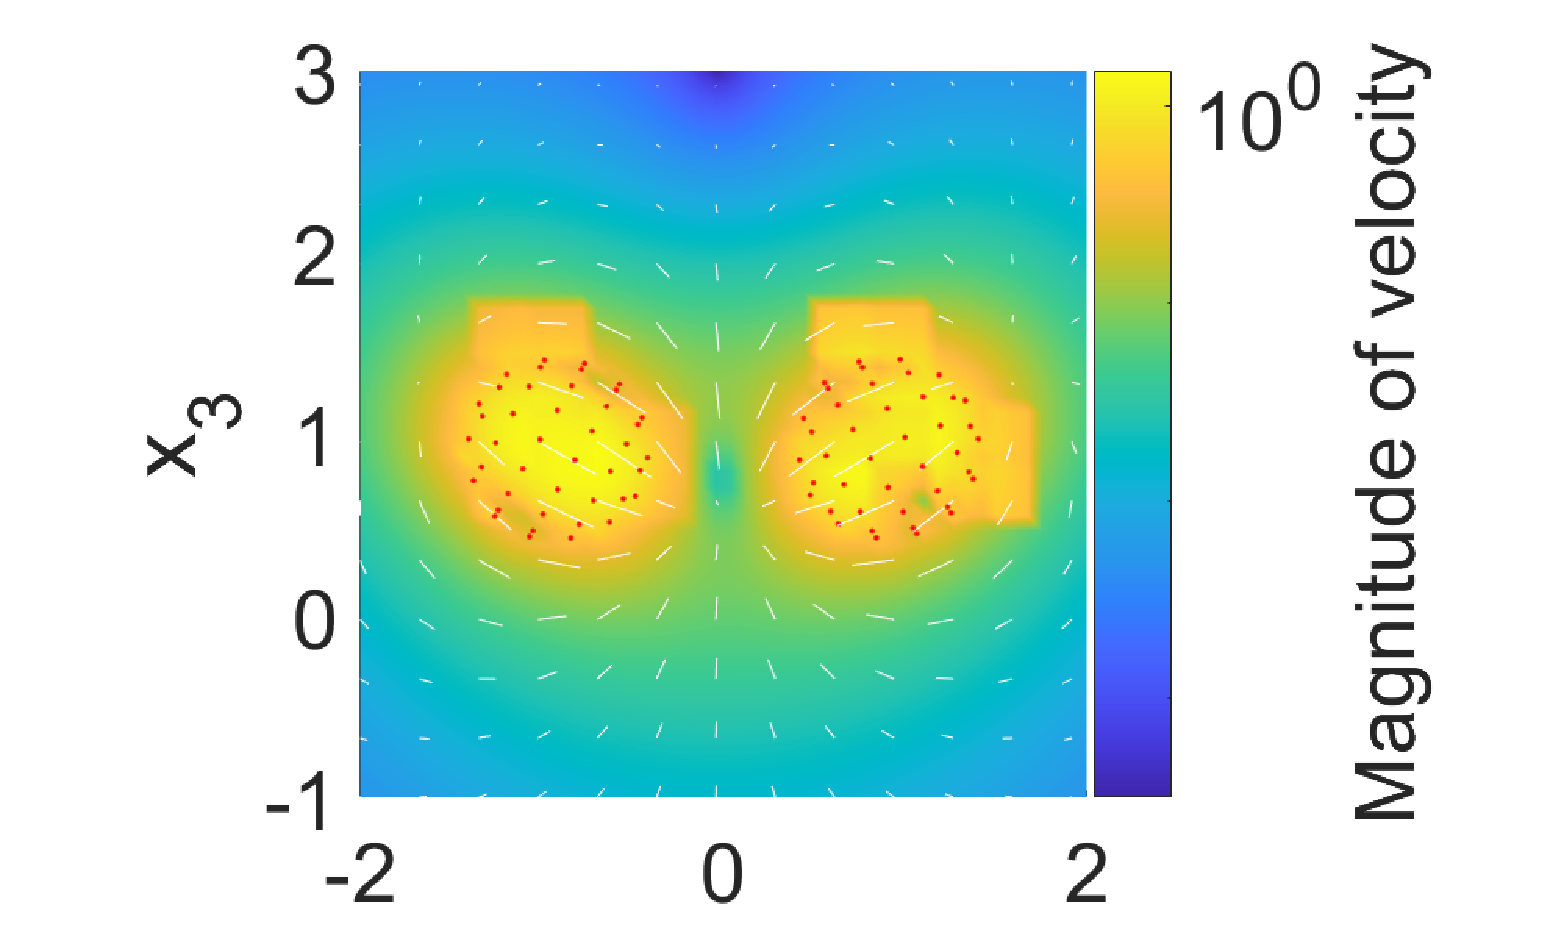
\includegraphics[width=\textwidth]{Images/squirmers/Pair-8.pdf}
    \caption[]{\label{fig:PairH}}
\end{subfigure}
\caption[Flow visualisation around a pair of squirmers.]{\label{fig:Squiremer3DFlowPair} Flow visualisation at a slice at $x_1=0$ for a pair of squirmers at various time steps. The coarse discretisation points of the squirmers are plotted in white along with the squirmers local vertical axis. (i-viii) are taken at slices in the simulation at times $t = 0, 0.29, 0.57, 0.86, 1.14, 1.43, 1.71 \text{ and } 2$ respectively.}
\vspace{-1pt}
\end{figure}

\subsection{Bottom-heavy squirmers} \label{subsec:BottomHeavySquirmers}

For larger simulations, the choice was made to study bottom-heavy squirmers in a gravitational field \cite{Ruhle2020EmergentGravity,BrumleyStabilitySquirmers,Pedley2016SphericalMicro-organisms}. It has been seen that bottom-heavy squirmers, where the centre of mass lies below the geometric centre of the sphere, form clusters which rise and fall when confined between two parallel plates \cite{Ruhle2020EmergentGravity}. Implementation of both gravity and bottom heaviness is easy due to the formulation of the swimming problem, we set $\bm{G}=[0,0,g]$ where $g$ is the strength of gravity in the  direction. The torque is therefore defined to be $\bm{T}_j =  m g r_0 ( -\bm{b}_j^{(3)} \times \bm{e}_z)$ for $j=1,...,N_{sw}$ where $m$ is the mass of the squirmer (taken to be 1), $r_0$ is the offset of the centre of mass from the geometric centre and $\bm{e_z}$ is a unit vector pointing in the positive $z$-direction. We scatter 50 squirmers of radius $0.5$ in the region $[-1.6\; 1.6] \times [-1.6\; 1.6] \times [1\; 4.5]$. Each squirmer starts in a random direction and with a maximum velocity of two on the equator of the sphere. In order to constrain the squirmers we define two walls one at $z=0$ and the other at $z=10$ each with a size of $10 \times 10$. In order to keep the total scalar degrees of freedom reasonable 26 force points and 206 fine quadrature points are placed over the surface of the sphere with an effective spacing of 0.328 and 0.1 respectively. The boundaries are discretised with 3808 force points and 62382 fine quadrature points with effective spacing of 0.25 and 0.0625 respectively. 

The simulation was run on (M1) with standard setting with each iteration taking on average 551 seconds to solve. The differently equation was solved using \textit{ode45} with a relative tolerance of $10^{-2}$, the simulation was ran from $t=0$ to $t=10$ requiring 524 time steps. Due to the adaptive nature of the ode 45 solver some timesteps required more than a single solve in order to archive the required accuracy and as such a total of 943 solves were required. This mean the overall computation time of the problem was 138 hours. We only plot the first half of the computation in \cref{fig:SquiremerGyro,fig:SquiremerGyroPo} due to the upper boundary not containing the squirmier and as such the squirmers do not display the expected behaviour \cite{Ruhle2020EmergentGravity}. These computation times are currently significantly higher than solving via direct methods at these system scales although our current KIFMM is not optimised for the use in iterative methods.  

\begin{figure}
\centering
\begin{subfigure}[b]{0.2\textwidth}
    \centering
    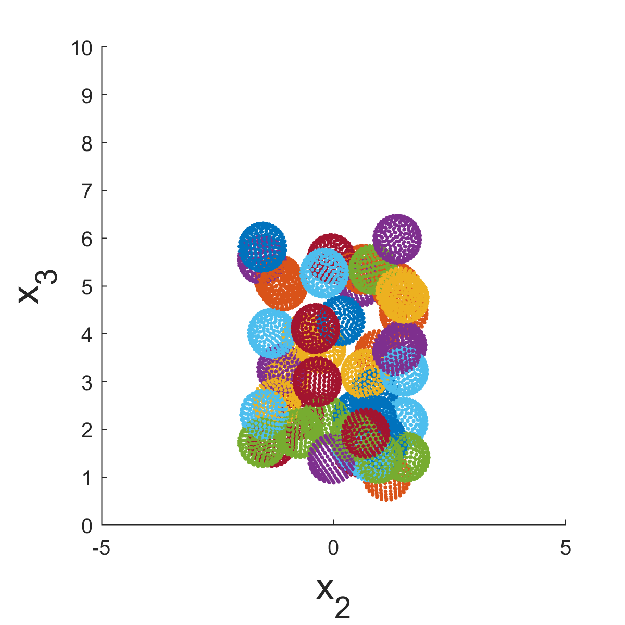
\includegraphics[width=\textwidth]{Images/squirmers/Gyro-1-All.pdf}
    \caption[]{\label{fig:squirmerPosA}} 
\end{subfigure} \hfill
\begin{subfigure}[b]{0.2\textwidth}
    \centering
    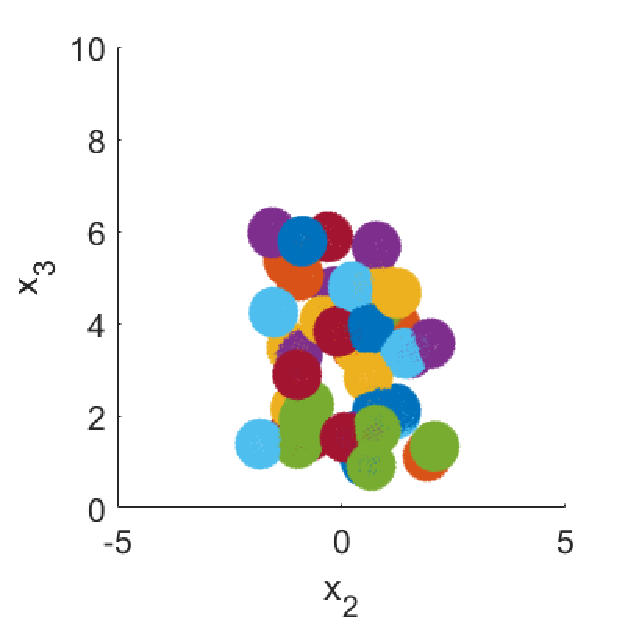
\includegraphics[width=\textwidth]{Images/squirmers/Gyro-2-All.pdf}
    \caption[]{\label{fig:squirmerPosB}}
\end{subfigure}\hfill
\begin{subfigure}[b]{0.2\textwidth}
    \centering
    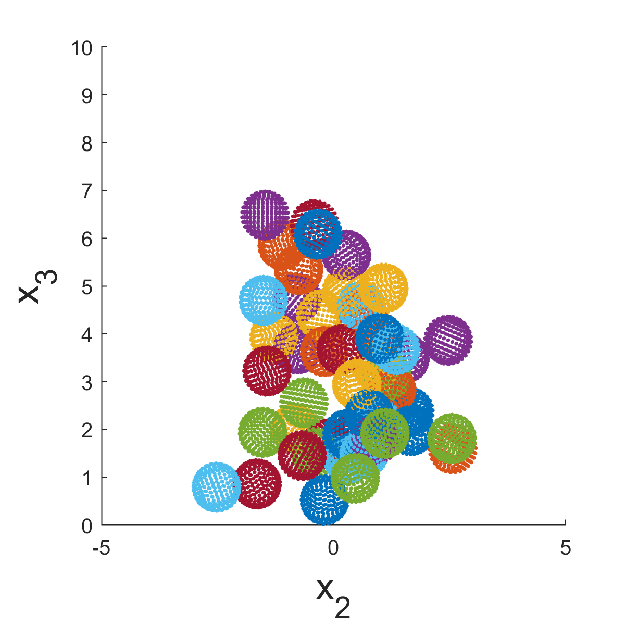
\includegraphics[width=\textwidth]{Images/squirmers/Gyro-3-All.pdf}
    \caption[]{\label{fig:squirmerPosC}}
\end{subfigure}\hfill
\begin{subfigure}[b]{0.2\textwidth}
    \centering
    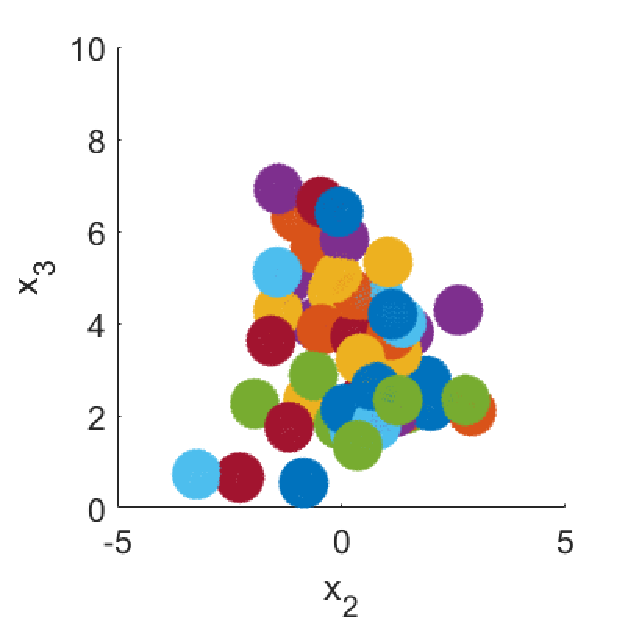
\includegraphics[width=\textwidth]{Images/squirmers/Gyro-4-All.pdf}
    \caption[]{\label{fig:squirmerPosD}}
\end{subfigure}
\vskip\baselineskip
\begin{subfigure}[b]{0.2\textwidth}
    \centering
    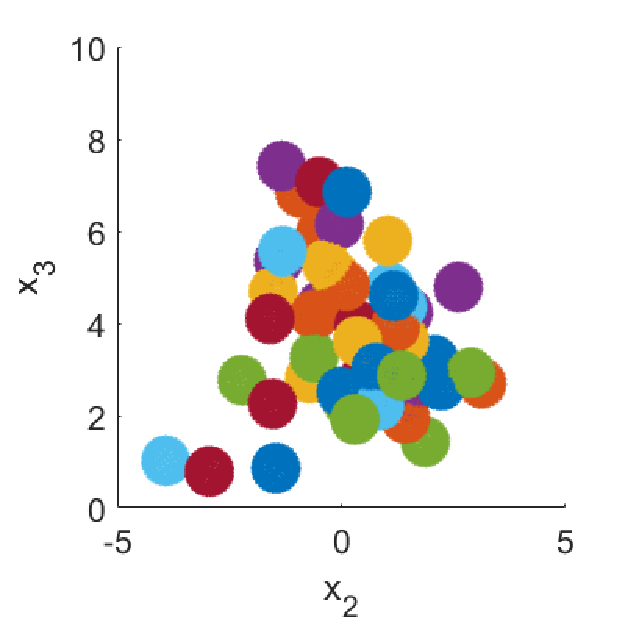
\includegraphics[width=\textwidth]{Images/squirmers/Gyro-5-All.pdf}
    \caption[]{\label{fig:squirmerPosE}}
\end{subfigure}\hfill
\begin{subfigure}[b]{0.2\textwidth}
    \centering
    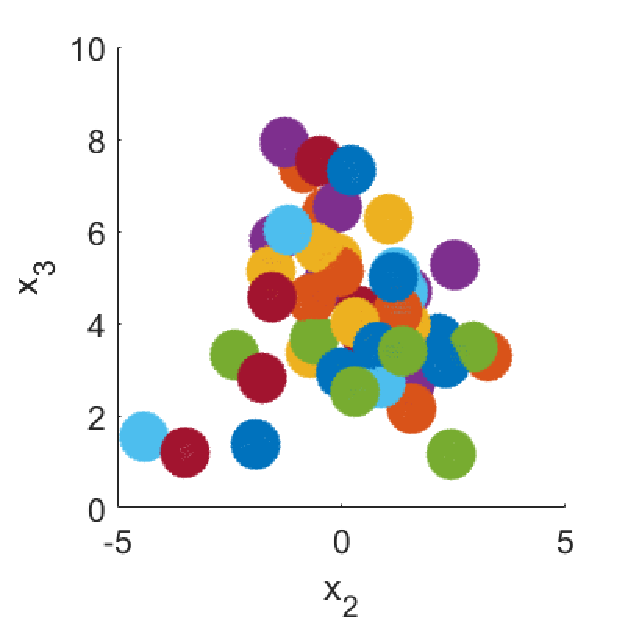
\includegraphics[width=\textwidth]{Images/squirmers/Gyro-6-All.pdf}
    \caption[]{\label{fig:squirmerPosF}}
\end{subfigure}\hfill
\begin{subfigure}[b]{0.2\textwidth}
    \centering
    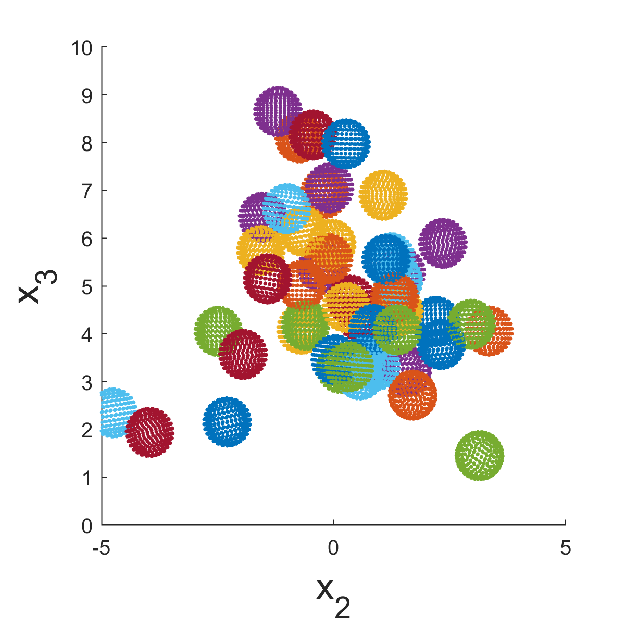
\includegraphics[width=\textwidth]{Images/squirmers/Gyro-7-All.pdf}
    \caption[]{\label{fig:squirmerPosG}}
\end{subfigure}\hfill
\begin{subfigure}[b]{0.2\textwidth}
    \centering
    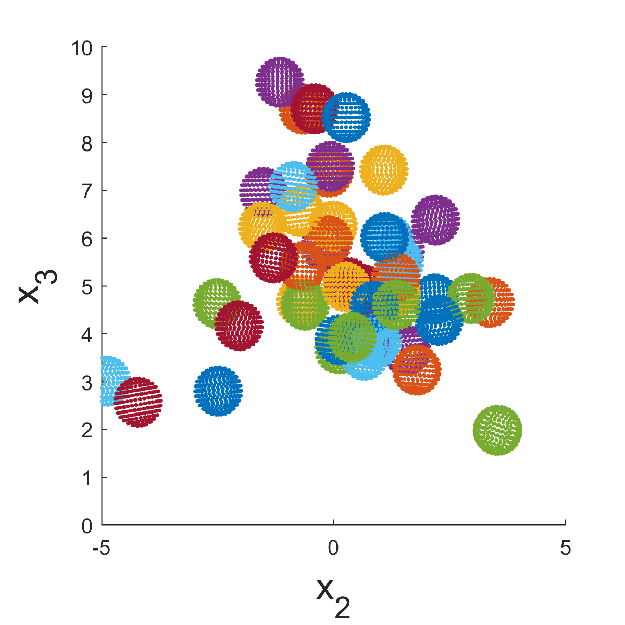
\includegraphics[width=\textwidth]{Images/squirmers/Gyro-8-All.pdf}
    \caption[]{\label{fig:squirmerPosH}}
\end{subfigure}
\label{fig:SquiremerGyroPo}
\caption[Position at 8 time steps of 50 squirmers randomly distributed at t=0.]{Position at 8 time steps of 50 squirmers randomly distributed at $t=0$. Two plates define the top and bottom of the simulations at $x_3 = 0$ and  $x_3 = 10$. (i-viii) show squirmer positions at $t = 0, 0.14, 0.29, 0.49, 0.57, 0.71, 0.86 \text{ and } 1$ respectively.}
\end{figure}

\begin{figure}
\centering
\begin{subfigure}[b]{0.42\textwidth}
    \centering
    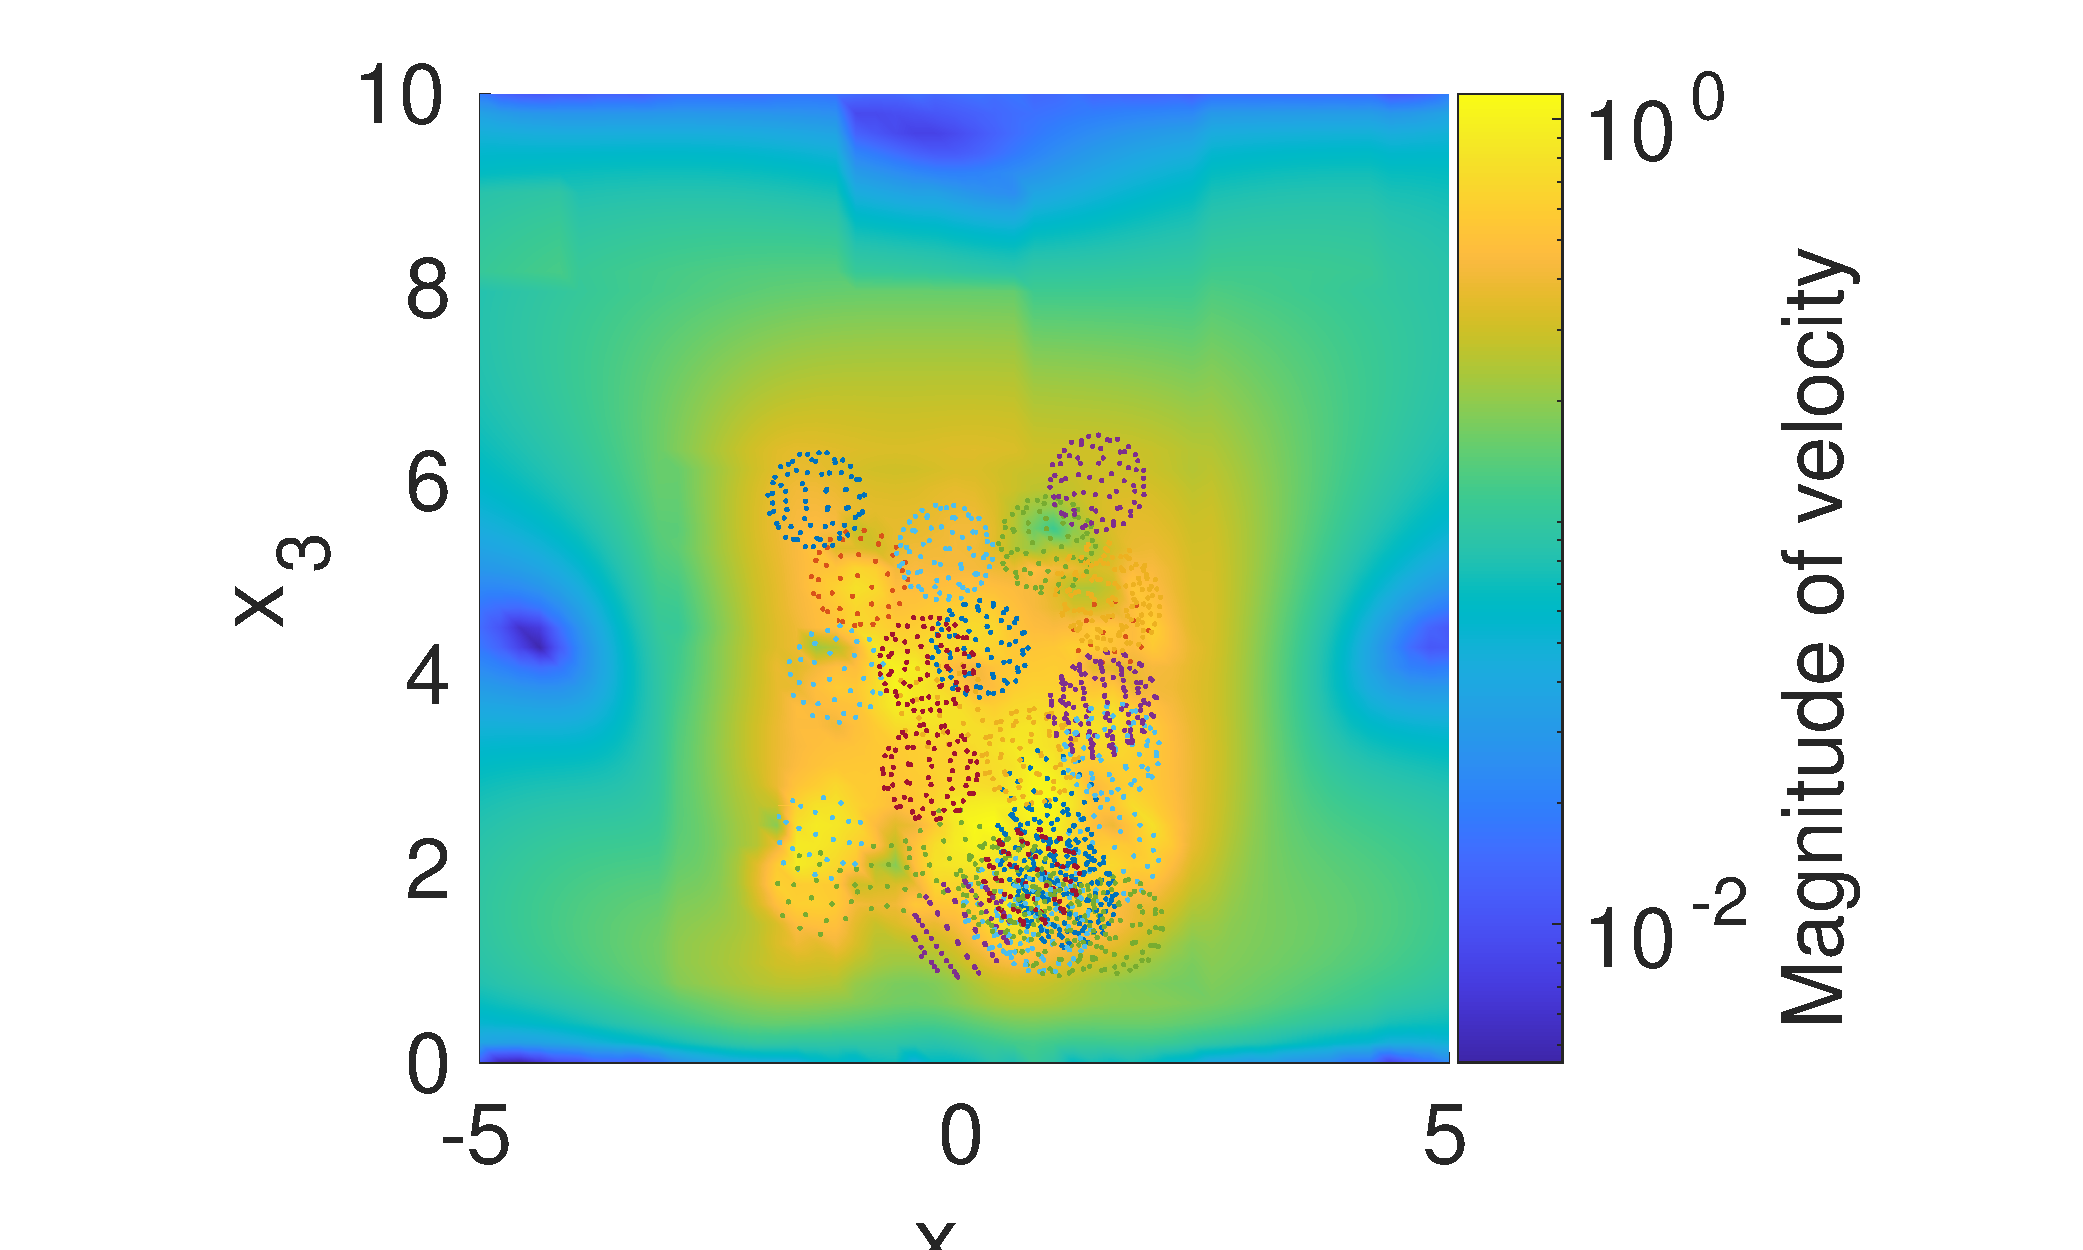
\includegraphics[width=\textwidth]{Images/squirmers/Gyro-1.pdf}
    \caption[]{\label{fig:squirmerA}}
\end{subfigure}
\begin{subfigure}[b]{0.42\textwidth}
    \centering
    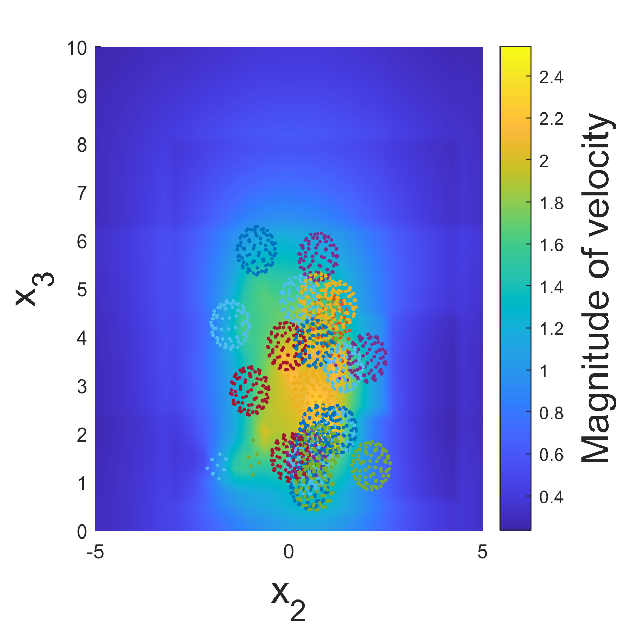
\includegraphics[width=\textwidth]{Images/squirmers/Gyro-2.pdf}
    \caption[]{\label{fig:squirmerB}}
\end{subfigure}
\begin{subfigure}[b]{0.42\textwidth}
    \centering
    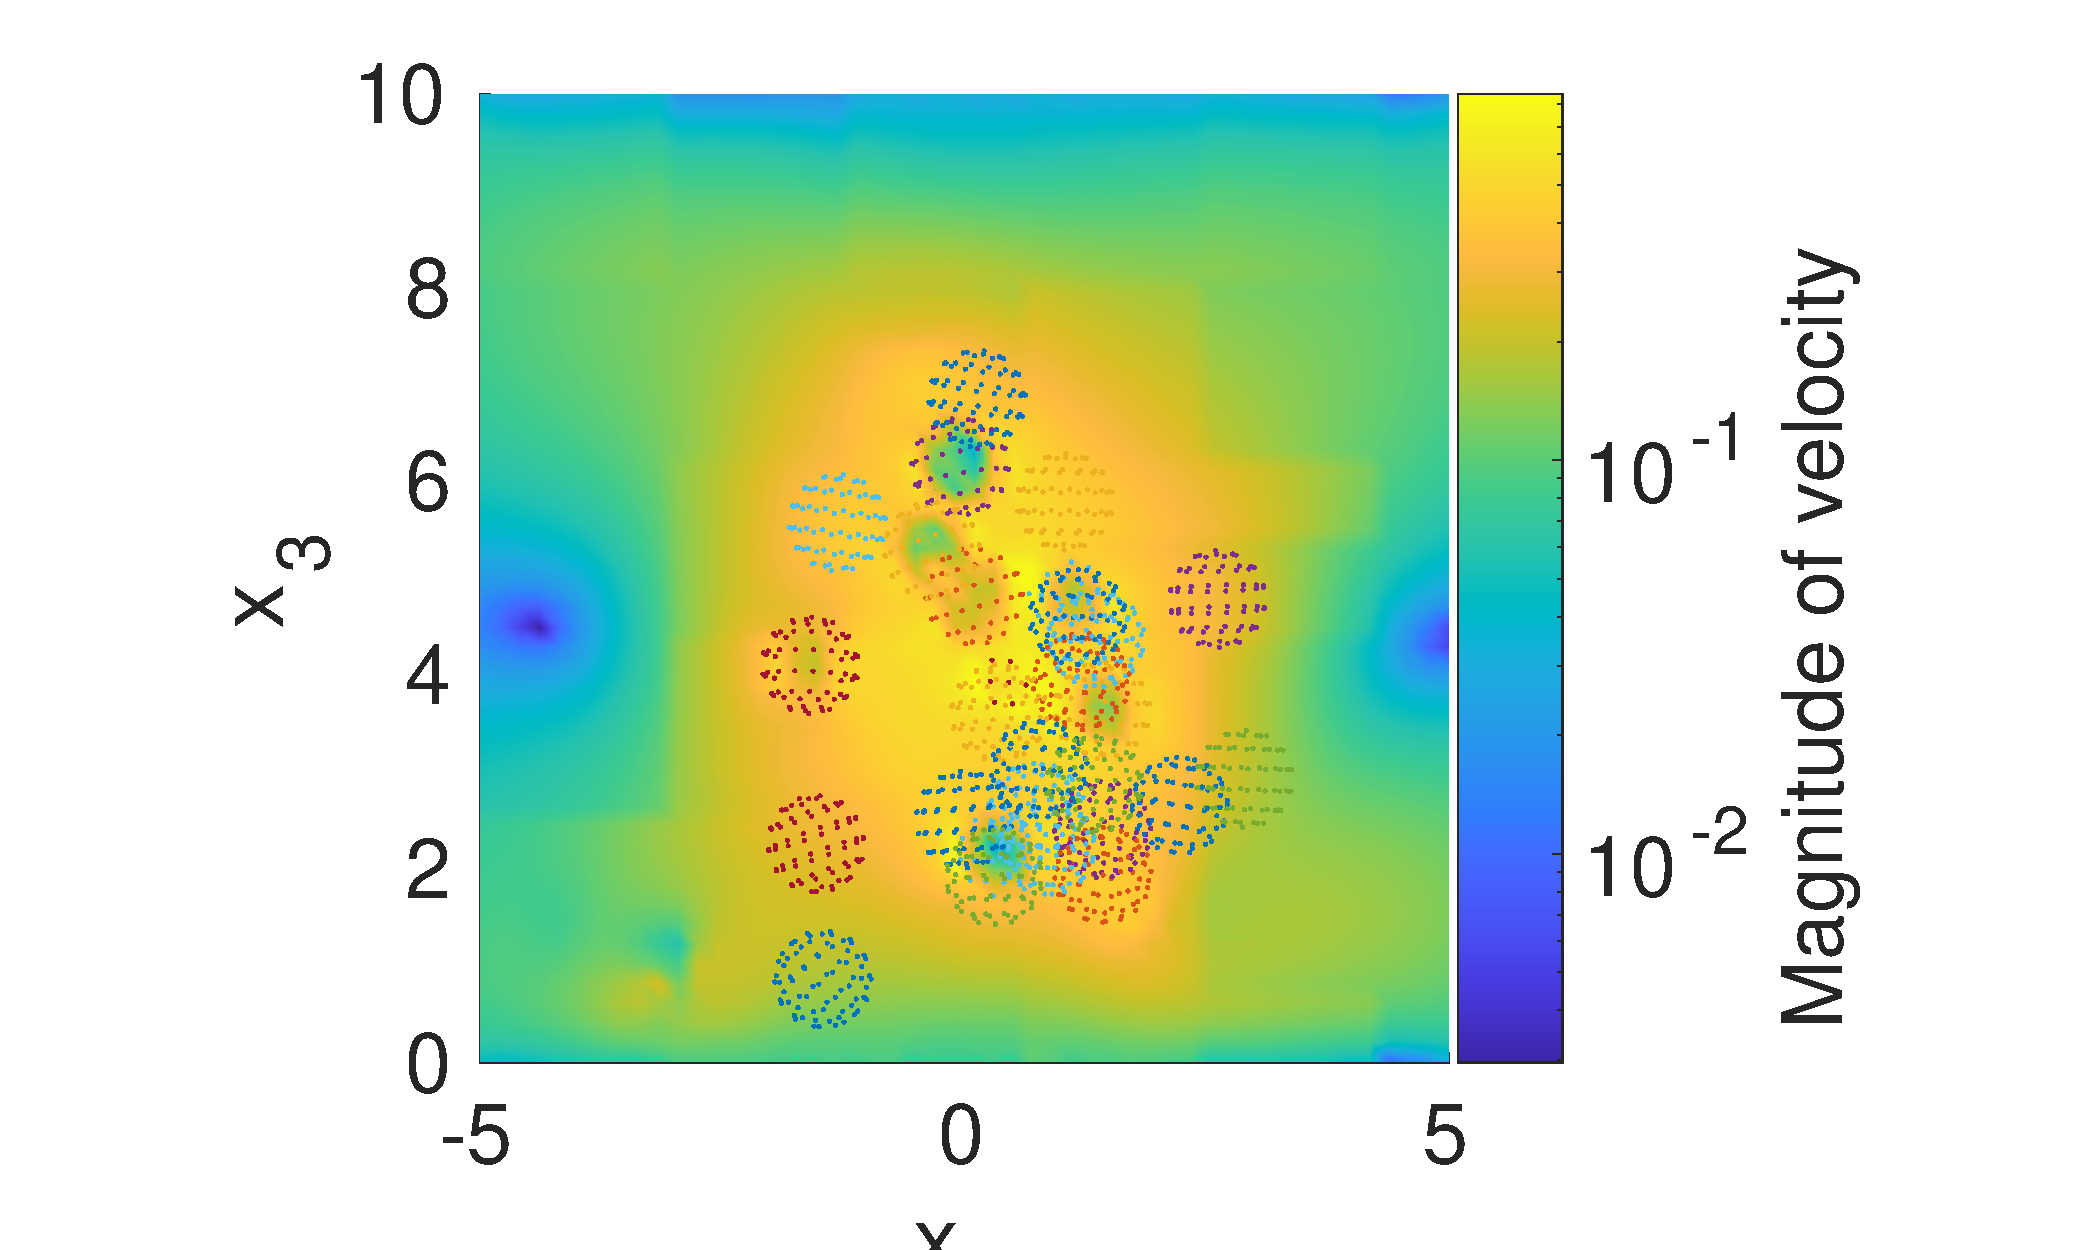
\includegraphics[width=\textwidth]{Images/squirmers/Gyro-3.pdf}
    \caption[]{\label{fig:squirmerC}}
\end{subfigure}
\begin{subfigure}[b]{0.42\textwidth}
    \centering
    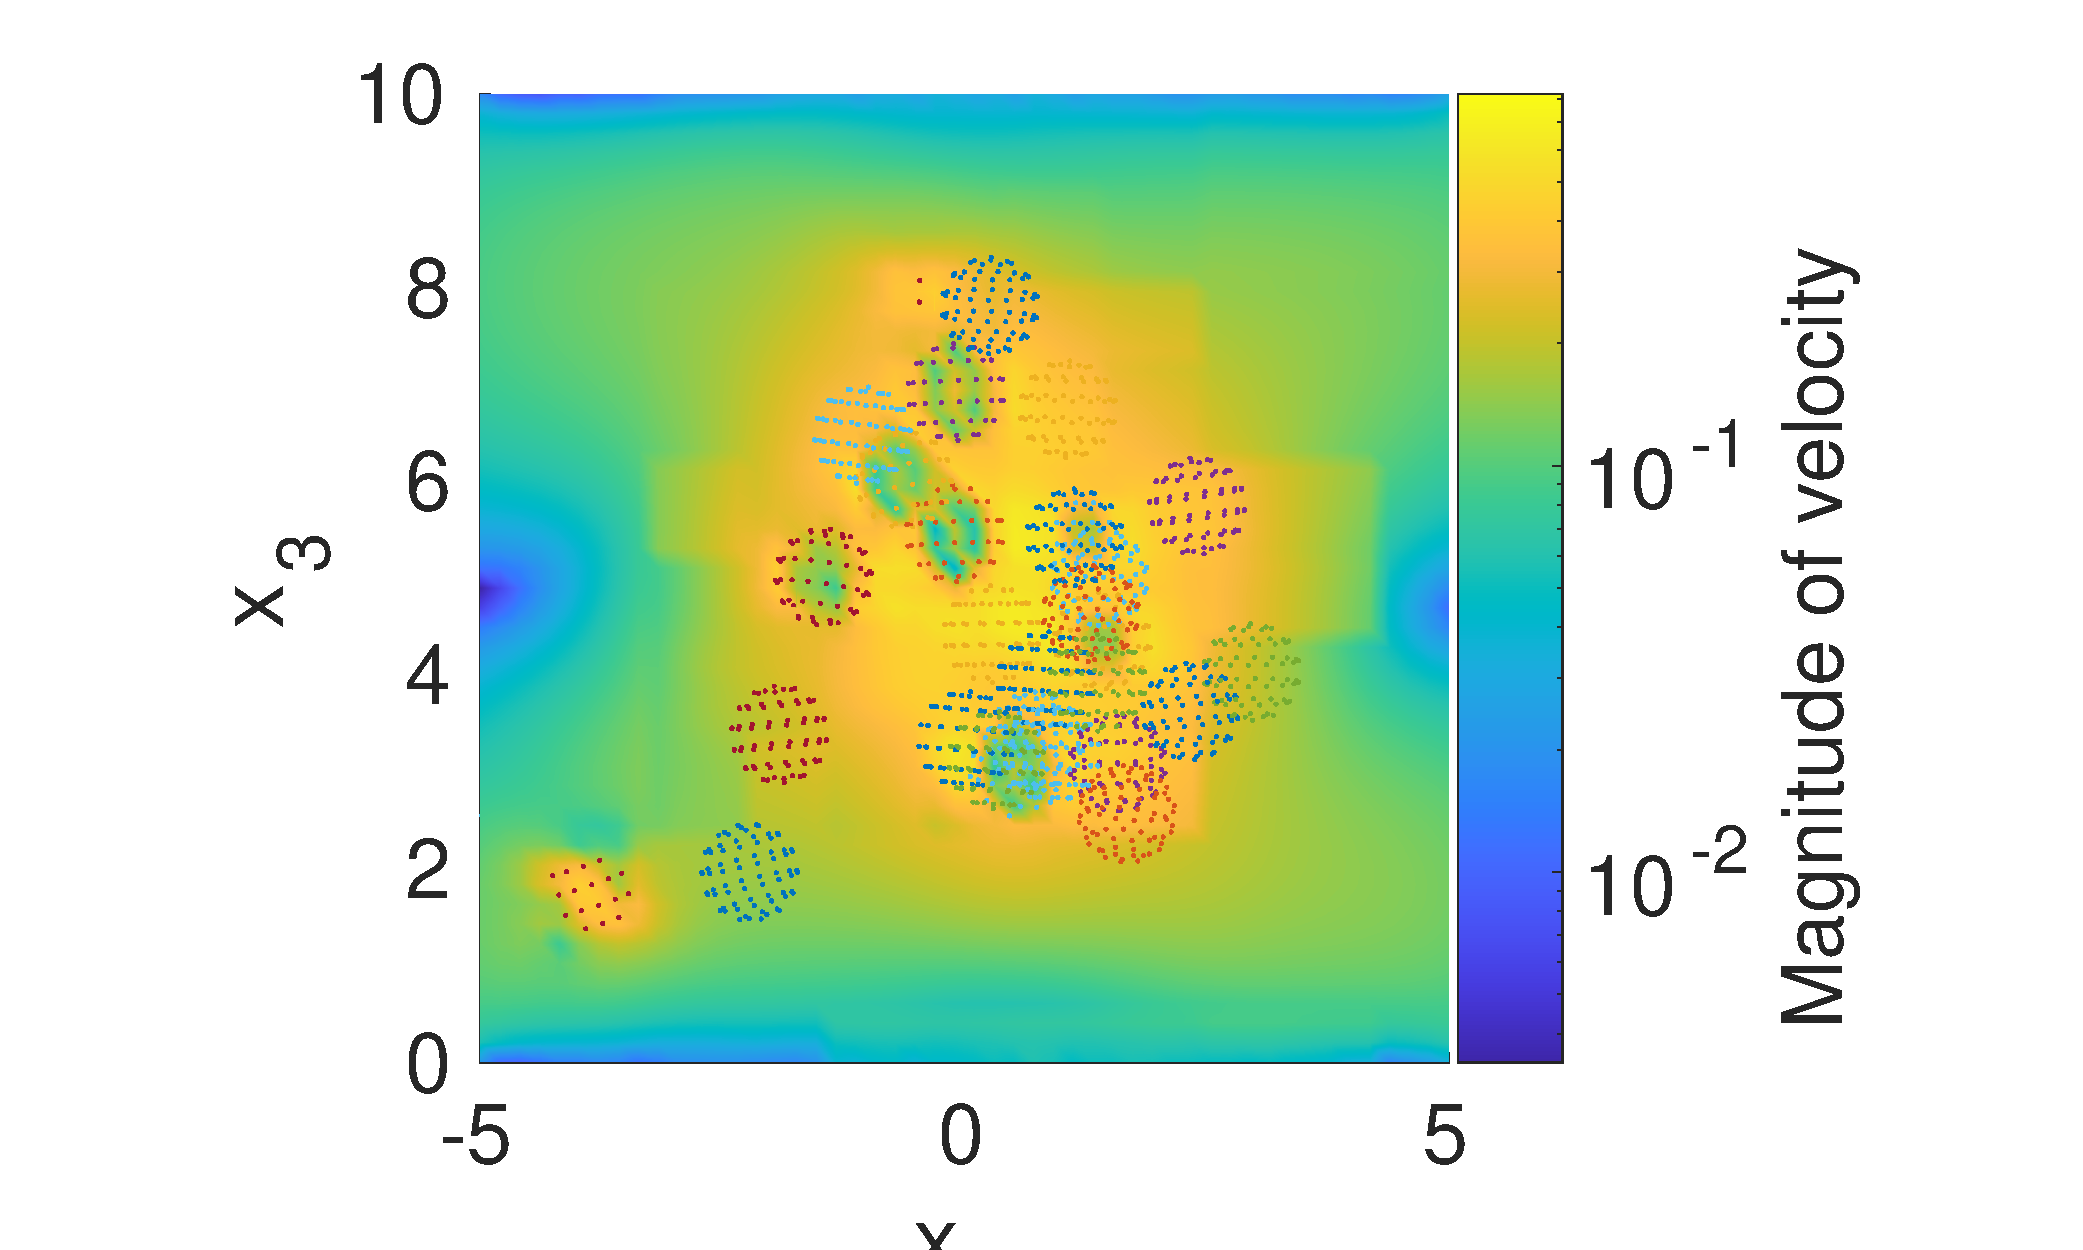
\includegraphics[width=\textwidth]{Images/squirmers/Gyro-4.pdf}
    \caption[]{\label{fig:squirmerD}}
\end{subfigure}
\vskip\baselineskip
\begin{subfigure}[b]{0.42\textwidth}
    \centering
    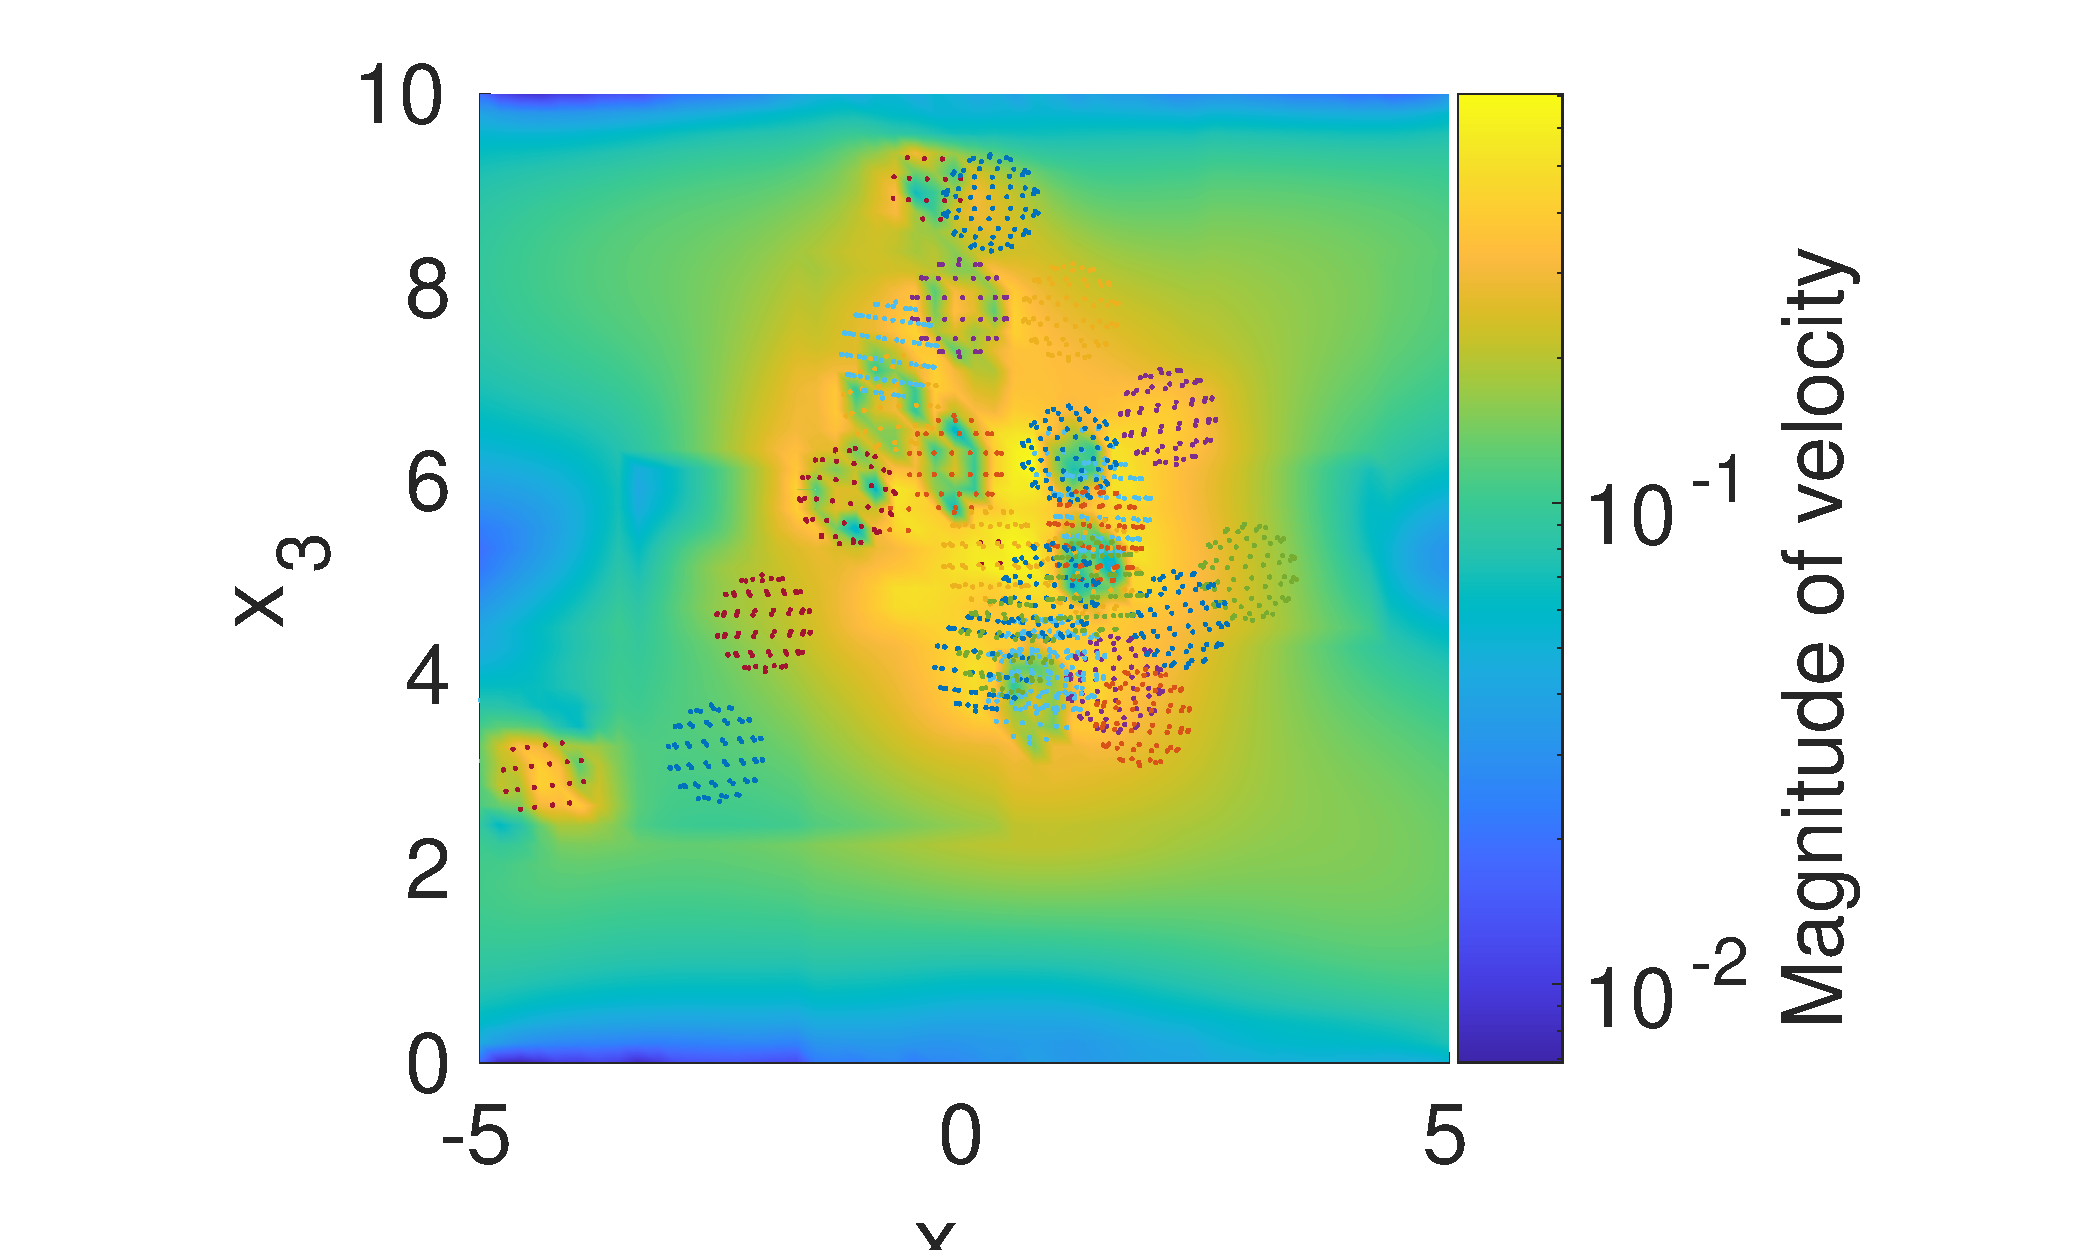
\includegraphics[width=\textwidth]{Images/squirmers/Gyro-5.pdf}
    \caption[]{\label{fig:squirmerE}}
\end{subfigure}
\begin{subfigure}[b]{0.42\textwidth}
    \centering
    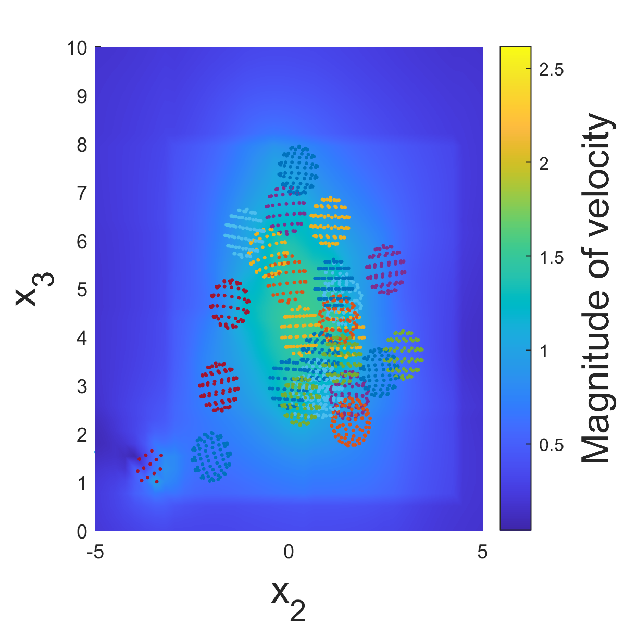
\includegraphics[width=\textwidth]{Images/squirmers/Gyro-6.pdf}
    \caption[]{\label{fig:squirmerF}}
\end{subfigure}
\begin{subfigure}[b]{0.42\textwidth}
    \centering
    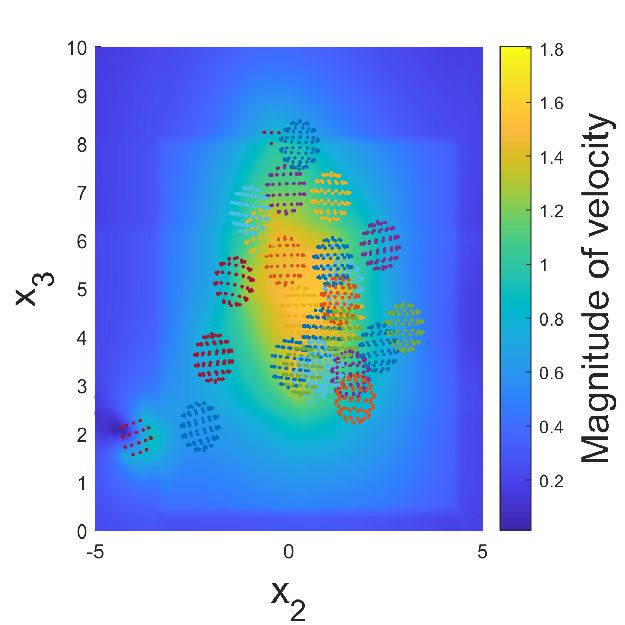
\includegraphics[width=\textwidth]{Images/squirmers/Gyro-7.pdf}
    \caption[]{\label{fig:squirmerG}}
\end{subfigure}
\begin{subfigure}[b]{0.42\textwidth}
    \centering
    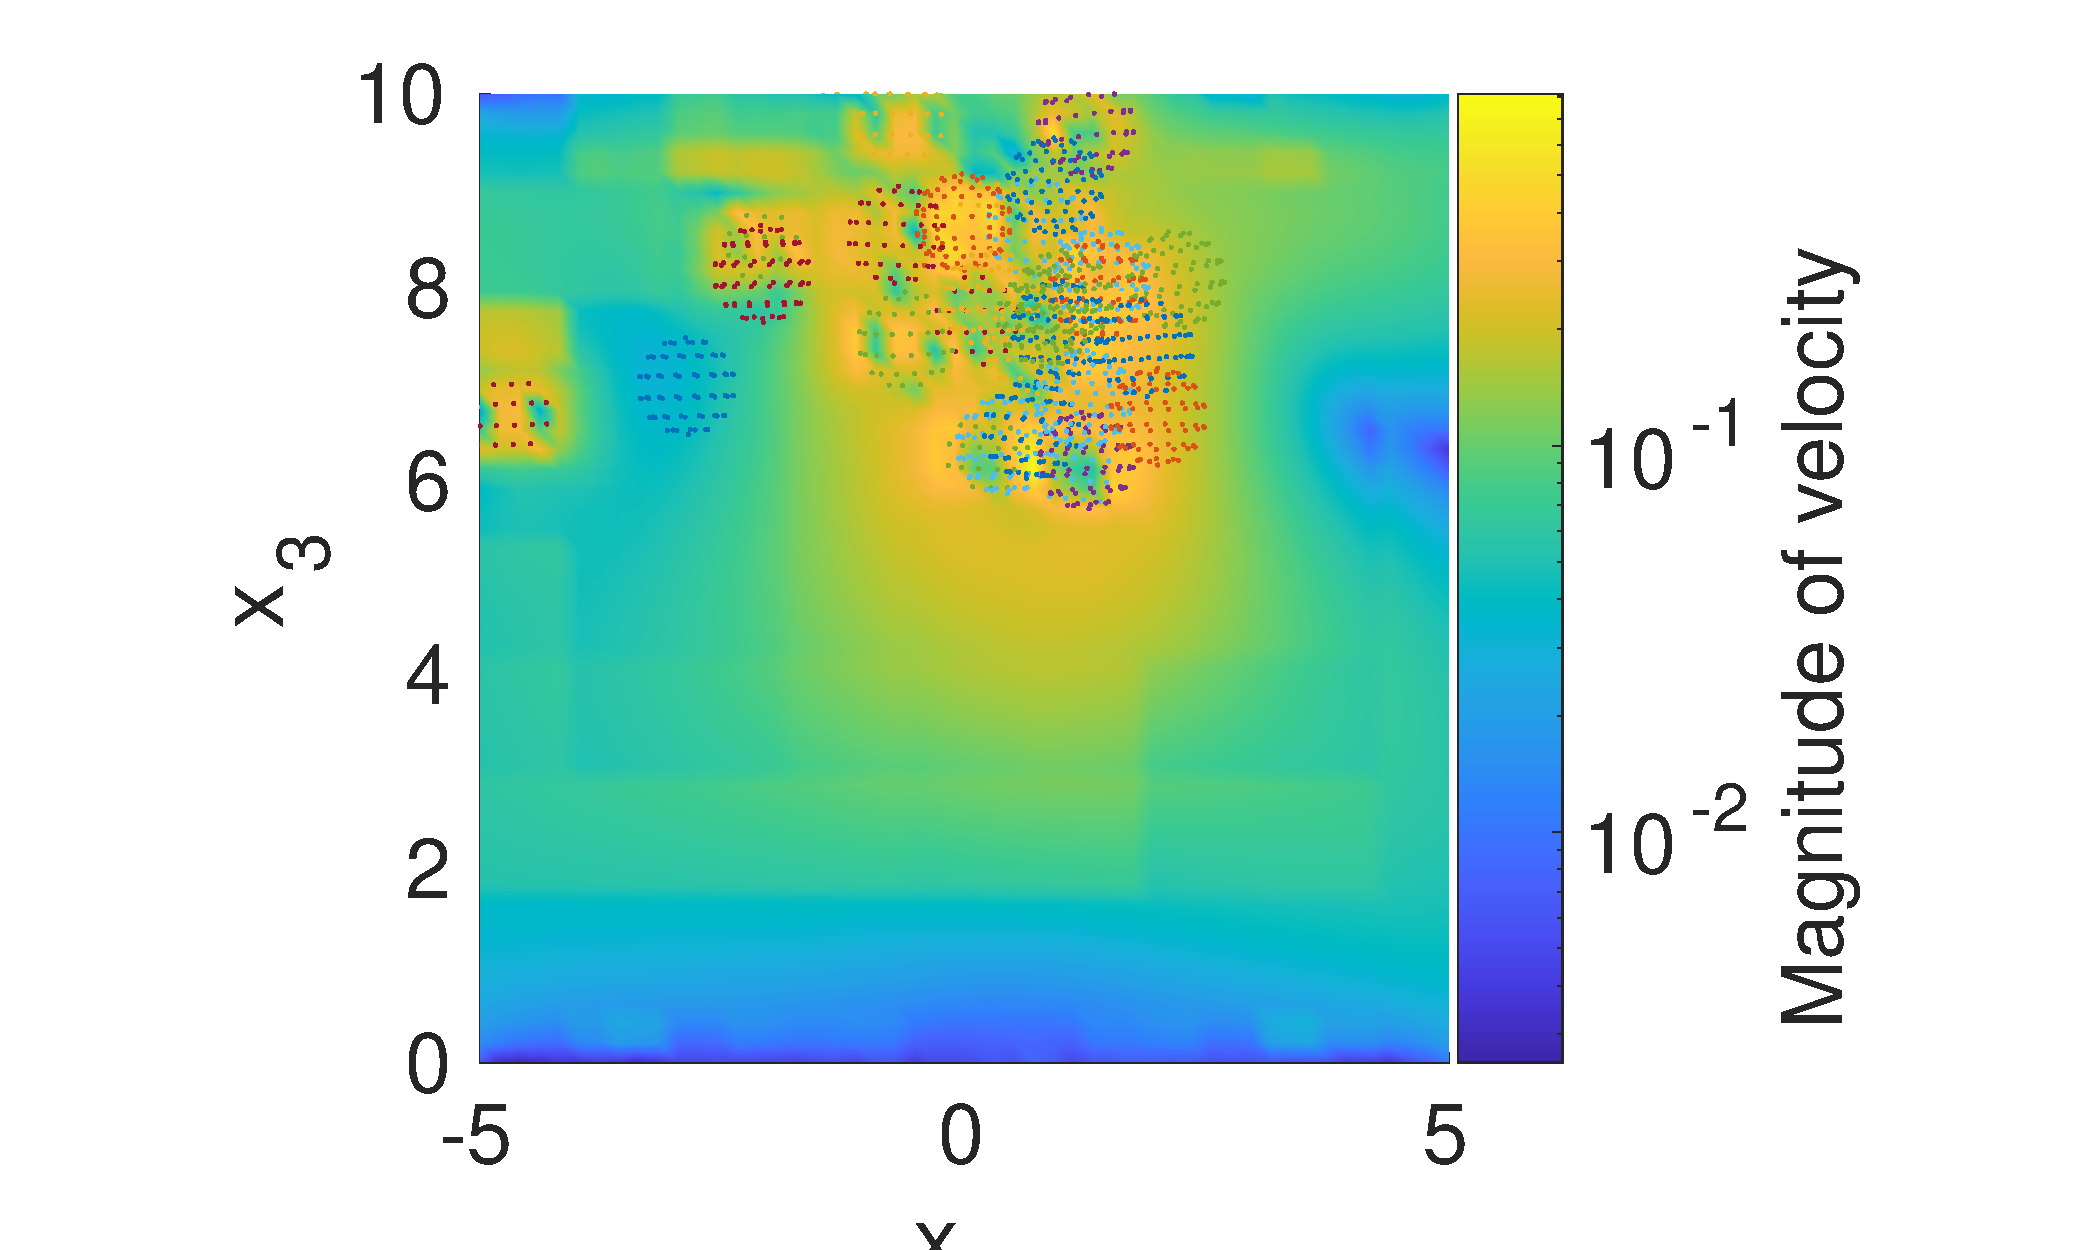
\includegraphics[width=\textwidth]{Images/squirmers/Gyro-8.pdf}
    \caption[]{\label{fig:squirmerH}}
\end{subfigure}
\label{fig:SquiremerGyro}
\caption[Position and velocity profile at 8 time steps of 50 squirmers randomly distributed at t=0.]{Position and velocity profile slice at $x_1=0$ are shown at 8 time steps of 50 squirmers randomly distributed at $t=0$. Two plates define the top and bottom of the simulations at $x_3 = 0$ and  $x_3 = 10$. (i-viii) show squirmer positions at $t = 0, 0.74, 1.48, 2.212, 2.96, 3.70, 4.44 \text{ and } 5.18$ respectively.}
\end{figure}

\section{Discussion}
\newpage
\appendix

\FloatBarrier

\pagestyle{contents}
\begin{singlespace}
\printbibliography[heading=bibintoc]
\end{singlespace}
\end{document}
